\documentclass[a4paper]{book}
\usepackage{a4wide}
\usepackage{makeidx}
\usepackage{graphicx}
\usepackage{multicol}
\usepackage{float}
\usepackage{listings}
\usepackage{color}
\usepackage{textcomp}
\usepackage{alltt}
\usepackage{times}
\usepackage{ifpdf}
\ifpdf
\usepackage[pdftex,
            pagebackref=true,
            colorlinks=true,
            linkcolor=blue,
            unicode
           ]{hyperref}
\else
\usepackage[ps2pdf,
            pagebackref=true,
            colorlinks=true,
            linkcolor=blue,
            unicode
           ]{hyperref}
\usepackage{pspicture}
\fi
\usepackage[utf8]{inputenc}
\usepackage{doxygen}
\lstset{language=C++,inputencoding=utf8,basicstyle=\footnotesize,breaklines=true,breakatwhitespace=true,tabsize=8,numbers=left }
\makeindex
\setcounter{tocdepth}{3}
\renewcommand{\footrulewidth}{0.4pt}
\begin{document}
\hypersetup{pageanchor=false}
\begin{titlepage}
\vspace*{7cm}
\begin{center}
{\Large Robosoccer }\\
\vspace*{1cm}
{\large Generated by Doxygen 1.6.3}\\
\vspace*{0.5cm}
{\small Wed Jul 15 11:51:29 2015}\\
\end{center}
\end{titlepage}
\clearemptydoublepage
\pagenumbering{roman}
\tableofcontents
\clearemptydoublepage
\pagenumbering{arabic}
\hypersetup{pageanchor=true}
\chapter{Class Index}
\section{Class Hierarchy}
This inheritance list is sorted roughly, but not completely, alphabetically:\begin{DoxyCompactList}
\item \contentsline{section}{BallMonitor::Angle}{\pageref{structBallMonitor_1_1Angle}}{}
\item \contentsline{section}{BallMonitor}{\pageref{classBallMonitor}}{}
\item \contentsline{section}{Button}{\pageref{structButton}}{}
\item \contentsline{section}{PathFinder::ConvexPolygon}{\pageref{structPathFinder_1_1ConvexPolygon}}{}
\item \contentsline{section}{CoordinatesCalibrer}{\pageref{classCoordinatesCalibrer}}{}
\item \contentsline{section}{BallMonitor::Direction}{\pageref{structBallMonitor_1_1Direction}}{}
\item \contentsline{section}{DragDrop}{\pageref{structDragDrop}}{}
\item \contentsline{section}{Matrix::FloodFillStruct}{\pageref{structMatrix_1_1FloodFillStruct}}{}
\item \contentsline{section}{Interpreter::GameData}{\pageref{structInterpreter_1_1GameData}}{}
\item \contentsline{section}{Interpreter}{\pageref{classInterpreter}}{}
\item \contentsline{section}{MainLoopDataStruct}{\pageref{structMainLoopDataStruct}}{}
\item \contentsline{section}{MapDisplay}{\pageref{classMapDisplay}}{}
\item \contentsline{section}{Matrix}{\pageref{classMatrix}}{}
\item \contentsline{section}{Matrix::MatrixProxy}{\pageref{classMatrix_1_1MatrixProxy}}{}
\item \contentsline{section}{node}{\pageref{classnode}}{}
\item \contentsline{section}{PathFinder}{\pageref{classPathFinder}}{}
\item \contentsline{section}{Interpreter::Point}{\pageref{structInterpreter_1_1Point}}{}
\item \contentsline{section}{PathFinder::Point}{\pageref{structPathFinder_1_1Point}}{}
\item \contentsline{section}{Matrix::Point}{\pageref{structMatrix_1_1Point}}{}
\item \contentsline{section}{BallMonitor::PosTime}{\pageref{structBallMonitor_1_1PosTime}}{}
\item \contentsline{section}{PathFinder::Rectangle}{\pageref{structPathFinder_1_1Rectangle}}{}
\item \contentsline{section}{RefereeDisplay}{\pageref{classRefereeDisplay}}{}
\item \contentsline{section}{RoboBall}{\pageref{structRoboBall}}{}
\item \contentsline{section}{RoboControl}{\pageref{classRoboControl}}{}
\begin{DoxyCompactList}
\item \contentsline{section}{NewRoboControl}{\pageref{classNewRoboControl}}{}
\begin{DoxyCompactList}
\item \contentsline{section}{OpponentRobot}{\pageref{classOpponentRobot}}{}
\item \contentsline{section}{TeamRobot}{\pageref{classTeamRobot}}{}
\begin{DoxyCompactList}
\item \contentsline{section}{Goalkeeper}{\pageref{classGoalkeeper}}{}
\item \contentsline{section}{PlayerMain}{\pageref{classPlayerMain}}{}
\item \contentsline{section}{PlayerTwo}{\pageref{classPlayerTwo}}{}
\end{DoxyCompactList}
\end{DoxyCompactList}
\end{DoxyCompactList}
\item \contentsline{section}{PathFinder::Segment}{\pageref{structPathFinder_1_1Segment}}{}
\end{DoxyCompactList}

\chapter{Class Index}
\section{Class List}
Here are the classes, structs, unions and interfaces with brief descriptions:\begin{DoxyCompactList}
\item\contentsline{section}{\hyperlink{structBallMonitor_1_1Angle}{BallMonitor::Angle} }{\pageref{structBallMonitor_1_1Angle}}{}
\item\contentsline{section}{\hyperlink{classBallMonitor}{BallMonitor} }{\pageref{classBallMonitor}}{}
\item\contentsline{section}{\hyperlink{structButton}{Button} }{\pageref{structButton}}{}
\item\contentsline{section}{\hyperlink{structPathFinder_1_1ConvexPolygon}{PathFinder::ConvexPolygon} (Structure used to represent a convex polygon )}{\pageref{structPathFinder_1_1ConvexPolygon}}{}
\item\contentsline{section}{\hyperlink{classCoordinatesCalibrer}{CoordinatesCalibrer} }{\pageref{classCoordinatesCalibrer}}{}
\item\contentsline{section}{\hyperlink{structBallMonitor_1_1Direction}{BallMonitor::Direction} }{\pageref{structBallMonitor_1_1Direction}}{}
\item\contentsline{section}{\hyperlink{structDragDrop}{DragDrop} }{\pageref{structDragDrop}}{}
\item\contentsline{section}{\hyperlink{structMatrix_1_1FloodFillStruct}{Matrix::FloodFillStruct} }{\pageref{structMatrix_1_1FloodFillStruct}}{}
\item\contentsline{section}{\hyperlink{structInterpreter_1_1GameData}{Interpreter::GameData} }{\pageref{structInterpreter_1_1GameData}}{}
\item\contentsline{section}{\hyperlink{classGoalkeeper}{Goalkeeper} }{\pageref{classGoalkeeper}}{}
\item\contentsline{section}{\hyperlink{classInterpreter}{Interpreter} }{\pageref{classInterpreter}}{}
\item\contentsline{section}{\hyperlink{structPlayerTwo_1_1KickParam}{PlayerTwo::KickParam} }{\pageref{structPlayerTwo_1_1KickParam}}{}
\item\contentsline{section}{\hyperlink{structMainLoopDataStruct}{MainLoopDataStruct} }{\pageref{structMainLoopDataStruct}}{}
\item\contentsline{section}{\hyperlink{classMapDisplay}{MapDisplay} }{\pageref{classMapDisplay}}{}
\item\contentsline{section}{\hyperlink{classMatrix}{Matrix} }{\pageref{classMatrix}}{}
\item\contentsline{section}{\hyperlink{classMatrix_1_1MatrixProxy}{Matrix::MatrixProxy} }{\pageref{classMatrix_1_1MatrixProxy}}{}
\item\contentsline{section}{\hyperlink{classNewRoboControl}{NewRoboControl} }{\pageref{classNewRoboControl}}{}
\item\contentsline{section}{\hyperlink{classnode}{node} }{\pageref{classnode}}{}
\item\contentsline{section}{\hyperlink{classOpponentRobot}{OpponentRobot} }{\pageref{classOpponentRobot}}{}
\item\contentsline{section}{\hyperlink{classPathFinder}{PathFinder} (Class used to find the shortest path in a given environment )}{\pageref{classPathFinder}}{}
\item\contentsline{section}{\hyperlink{classPlayerMain}{PlayerMain} }{\pageref{classPlayerMain}}{}
\item\contentsline{section}{\hyperlink{classPlayerTwo}{PlayerTwo} }{\pageref{classPlayerTwo}}{}
\item\contentsline{section}{\hyperlink{structInterpreter_1_1Point}{Interpreter::Point} }{\pageref{structInterpreter_1_1Point}}{}
\item\contentsline{section}{\hyperlink{structMatrix_1_1Point}{Matrix::Point} }{\pageref{structMatrix_1_1Point}}{}
\item\contentsline{section}{\hyperlink{structPathFinder_1_1Point}{PathFinder::Point} (Structure to represent a point in the path finder )}{\pageref{structPathFinder_1_1Point}}{}
\item\contentsline{section}{\hyperlink{structBallMonitor_1_1PosTime}{BallMonitor::PosTime} }{\pageref{structBallMonitor_1_1PosTime}}{}
\item\contentsline{section}{\hyperlink{structPathFinder_1_1Rectangle}{PathFinder::Rectangle} (Structure used to represent a horizontal rectangle )}{\pageref{structPathFinder_1_1Rectangle}}{}
\item\contentsline{section}{\hyperlink{classRefereeDisplay}{RefereeDisplay} }{\pageref{classRefereeDisplay}}{}
\item\contentsline{section}{\hyperlink{structRoboBall}{RoboBall} }{\pageref{structRoboBall}}{}
\item\contentsline{section}{\hyperlink{structPathFinder_1_1Segment}{PathFinder::Segment} (Structure used to describe a line segment )}{\pageref{structPathFinder_1_1Segment}}{}
\item\contentsline{section}{\hyperlink{classTeamRobot}{TeamRobot} }{\pageref{classTeamRobot}}{}
\end{DoxyCompactList}

\chapter{File Index}
\section{File List}
Here is a list of all files with brief descriptions:\begin{DoxyCompactList}
\item\contentsline{section}{src/\hyperlink{ballmonitor_8cpp}{ballmonitor.cpp} }{\pageref{ballmonitor_8cpp}}{}
\item\contentsline{section}{src/\hyperlink{ballmonitor_8h}{ballmonitor.h} }{\pageref{ballmonitor_8h}}{}
\item\contentsline{section}{src/\hyperlink{coordinates_8cpp}{coordinates.cpp} }{\pageref{coordinates_8cpp}}{}
\item\contentsline{section}{src/\hyperlink{coordinates_8h}{coordinates.h} }{\pageref{coordinates_8h}}{}
\item\contentsline{section}{src/\hyperlink{geometry_8cpp}{geometry.cpp} }{\pageref{geometry_8cpp}}{}
\item\contentsline{section}{src/\hyperlink{geometry_8h}{geometry.h} }{\pageref{geometry_8h}}{}
\item\contentsline{section}{src/\hyperlink{goalkeeper_8cpp}{goalkeeper.cpp} }{\pageref{goalkeeper_8cpp}}{}
\item\contentsline{section}{src/\hyperlink{goalkeeper_8h}{goalkeeper.h} }{\pageref{goalkeeper_8h}}{}
\item\contentsline{section}{src/\hyperlink{interpreter_8cpp}{interpreter.cpp} }{\pageref{interpreter_8cpp}}{}
\item\contentsline{section}{src/\hyperlink{interpreter_8h}{interpreter.h} }{\pageref{interpreter_8h}}{}
\item\contentsline{section}{src/\hyperlink{log_8cpp}{log.cpp} }{\pageref{log_8cpp}}{}
\item\contentsline{section}{src/\hyperlink{log_8h}{log.h} }{\pageref{log_8h}}{}
\item\contentsline{section}{src/\hyperlink{main_8cpp}{main.cpp} }{\pageref{main_8cpp}}{}
\item\contentsline{section}{src/\hyperlink{mapdisplay_8cpp}{mapdisplay.cpp} }{\pageref{mapdisplay_8cpp}}{}
\item\contentsline{section}{src/\hyperlink{mapdisplay_8h}{mapdisplay.h} }{\pageref{mapdisplay_8h}}{}
\item\contentsline{section}{src/\hyperlink{matrix_8cpp}{matrix.cpp} }{\pageref{matrix_8cpp}}{}
\item\contentsline{section}{src/\hyperlink{matrix_8h}{matrix.h} }{\pageref{matrix_8h}}{}
\item\contentsline{section}{src/\hyperlink{mutexdebug_8h}{mutexdebug.h} }{\pageref{mutexdebug_8h}}{}
\item\contentsline{section}{src/\hyperlink{newrobocontrol_8cpp}{newrobocontrol.cpp} }{\pageref{newrobocontrol_8cpp}}{}
\item\contentsline{section}{src/\hyperlink{newrobocontrol_8h}{newrobocontrol.h} }{\pageref{newrobocontrol_8h}}{}
\item\contentsline{section}{src/\hyperlink{node_8cpp}{node.cpp} }{\pageref{node_8cpp}}{}
\item\contentsline{section}{src/\hyperlink{node_8h}{node.h} }{\pageref{node_8h}}{}
\item\contentsline{section}{src/\hyperlink{opponentrobot_8cpp}{opponentrobot.cpp} }{\pageref{opponentrobot_8cpp}}{}
\item\contentsline{section}{src/\hyperlink{opponentrobot_8h}{opponentrobot.h} }{\pageref{opponentrobot_8h}}{}
\item\contentsline{section}{src/\hyperlink{pathfinder_8cpp}{pathfinder.cpp} }{\pageref{pathfinder_8cpp}}{}
\item\contentsline{section}{src/\hyperlink{pathfinder_8h}{pathfinder.h} }{\pageref{pathfinder_8h}}{}
\item\contentsline{section}{src/\hyperlink{playermain_8cpp}{playermain.cpp} }{\pageref{playermain_8cpp}}{}
\item\contentsline{section}{src/\hyperlink{playermain_8h}{playermain.h} }{\pageref{playermain_8h}}{}
\item\contentsline{section}{src/\hyperlink{playertwo_8cpp}{playertwo.cpp} }{\pageref{playertwo_8cpp}}{}
\item\contentsline{section}{src/\hyperlink{playertwo_8h}{playertwo.h} }{\pageref{playertwo_8h}}{}
\item\contentsline{section}{src/\hyperlink{refereedisplay_8cpp}{refereedisplay.cpp} }{\pageref{refereedisplay_8cpp}}{}
\item\contentsline{section}{src/\hyperlink{refereedisplay_8h}{refereedisplay.h} }{\pageref{refereedisplay_8h}}{}
\item\contentsline{section}{src/\hyperlink{sdlutilities_8cpp}{sdlutilities.cpp} }{\pageref{sdlutilities_8cpp}}{}
\item\contentsline{section}{src/\hyperlink{sdlutilities_8h}{sdlutilities.h} }{\pageref{sdlutilities_8h}}{}
\item\contentsline{section}{src/\hyperlink{standardfsm_8cpp}{standardfsm.cpp} }{\pageref{standardfsm_8cpp}}{}
\item\contentsline{section}{src/\hyperlink{standardfsm_8h}{standardfsm.h} }{\pageref{standardfsm_8h}}{}
\item\contentsline{section}{src/\hyperlink{teamrobot_8cpp}{teamrobot.cpp} }{\pageref{teamrobot_8cpp}}{}
\item\contentsline{section}{src/\hyperlink{teamrobot_8h}{teamrobot.h} }{\pageref{teamrobot_8h}}{}
\end{DoxyCompactList}

\chapter{Class Documentation}
\hypertarget{structBallMonitor_1_1Angle}{
\section{BallMonitor::Angle Struct Reference}
\label{structBallMonitor_1_1Angle}\index{BallMonitor::Angle@{BallMonitor::Angle}}
}


Describes an angle.  


\subsection*{Public Attributes}
\begin{DoxyCompactItemize}
\item 
double \hyperlink{structBallMonitor_1_1Angle_a78fc53a17705399300e15527aa9797dc}{val}
\item 
int \hyperlink{structBallMonitor_1_1Angle_a8c4cf98ad8b22adcc0bf58bd575185bf}{id}
\end{DoxyCompactItemize}


\subsection{Detailed Description}
Describes an angle. 

\subsection{Member Data Documentation}
\hypertarget{structBallMonitor_1_1Angle_a8c4cf98ad8b22adcc0bf58bd575185bf}{
\index{BallMonitor::Angle@{BallMonitor::Angle}!id@{id}}
\index{id@{id}!BallMonitor::Angle@{BallMonitor::Angle}}
\subsubsection[{id}]{\setlength{\rightskip}{0pt plus 5cm}int {\bf BallMonitor::Angle::id}}}
\label{structBallMonitor_1_1Angle_a8c4cf98ad8b22adcc0bf58bd575185bf}
The ID of the angle \hypertarget{structBallMonitor_1_1Angle_a78fc53a17705399300e15527aa9797dc}{
\index{BallMonitor::Angle@{BallMonitor::Angle}!val@{val}}
\index{val@{val}!BallMonitor::Angle@{BallMonitor::Angle}}
\subsubsection[{val}]{\setlength{\rightskip}{0pt plus 5cm}double {\bf BallMonitor::Angle::val}}}
\label{structBallMonitor_1_1Angle_a78fc53a17705399300e15527aa9797dc}
The angle value (in radians) 

The documentation for this struct was generated from the following file:\begin{DoxyCompactItemize}
\item 
src/\hyperlink{ballmonitor_8h}{ballmonitor.h}\end{DoxyCompactItemize}

\hypertarget{classBallMonitor}{
\section{BallMonitor Class Reference}
\label{classBallMonitor}\index{BallMonitor@{BallMonitor}}
}


{\ttfamily \#include $<$ballmonitor.h$>$}

\subsection*{Classes}
\begin{DoxyCompactItemize}
\item 
struct \hyperlink{structBallMonitor_1_1Angle}{Angle}
\begin{DoxyCompactList}\small\item\em This structure contains the value and is of an angle. \item\end{DoxyCompactList}\item 
struct \hyperlink{structBallMonitor_1_1Direction}{Direction}
\begin{DoxyCompactList}\small\item\em This structure contains the direction coordinates of the ball. \item\end{DoxyCompactList}\item 
struct \hyperlink{structBallMonitor_1_1PosTime}{PosTime}
\begin{DoxyCompactList}\small\item\em This structure contains the position of the ball and the given time. \item\end{DoxyCompactList}\end{DoxyCompactItemize}
\subsection*{Public Member Functions}
\begin{DoxyCompactItemize}
\item 
\hyperlink{classBallMonitor_a176a257973eefa572b6972aa6b5a605d}{BallMonitor} (\hyperlink{classCoordinatesCalibrer}{CoordinatesCalibrer} $\ast$coordCalibrer, RawBall $\ast$ball=NULL)
\begin{DoxyCompactList}\small\item\em creates a \hyperlink{classBallMonitor}{BallMonitor} . This is the constructor of ball monitor class \item\end{DoxyCompactList}\item 
bool \hyperlink{classBallMonitor_a4d2b3aa764f5d4f4d5f58b7530565f90}{StartMonitoring} (RawBall $\ast$ball=NULL)
\begin{DoxyCompactList}\small\item\em This function starts the monitoring of the ball.It creates a new thread to monitor the ball. \item\end{DoxyCompactList}\item 
bool \hyperlink{classBallMonitor_af71db12abeb1f10f7be58eb7591910a3}{StopMonitoring} ()
\begin{DoxyCompactList}\small\item\em This function stops the monitoring of the ball.It destroys the thread created to monitor the ball. \item\end{DoxyCompactList}\item 
bool \hyperlink{classBallMonitor_aab81815271c442087c15bc8f6843d092}{GetBallPosition} (Position $\ast$pos) const 
\begin{DoxyCompactList}\small\item\em This function gets the position of the ball. \item\end{DoxyCompactList}\item 
bool \hyperlink{classBallMonitor_a3cd2fe1ed297c468634fbb390ca088bd}{GetBallDirection} (\hyperlink{structBallMonitor_1_1Direction}{Direction} $\ast$dir) const 
\begin{DoxyCompactList}\small\item\em This function gets the direction of the ball. \item\end{DoxyCompactList}\item 
bool \hyperlink{classBallMonitor_a914053314023ea79ee691a3031e355bf}{PredictBallPosition} (double $\ast$a, double $\ast$b, int precision)
\begin{DoxyCompactList}\small\item\em This funtion predicts the linear trajectory of a moving ball with a certain precision based on two positions of the ball in two different times. \item\end{DoxyCompactList}\item 
bool \hyperlink{classBallMonitor_a8995e71b82d80987984dd6b1ed89c0a0}{IsBallMoving} () const 
\begin{DoxyCompactList}\small\item\em Tells if the ball is moving on the field or not. \item\end{DoxyCompactList}\item 
std::vector$<$ double $>$ \hyperlink{classBallMonitor_aad046acf9df6b0381ab3b1b8351e97c5}{ComputeVisibilityMap} (int maxLevel, const \hyperlink{classNewRoboControl}{NewRoboControl} $\ast$robot\mbox{[}6\mbox{]}, eSide ourSide, const \hyperlink{classCoordinatesCalibrer}{CoordinatesCalibrer} $\ast$coordCalib) const 
\begin{DoxyCompactList}\small\item\em This function computes the visibility map based on the position of other robots and on our side. \item\end{DoxyCompactList}\item 
std::vector$<$ double $>$ \hyperlink{classBallMonitor_ac30119e22cfe4814670c4eae8c6b5495}{ComputeVisibilityMap} (const \hyperlink{classNewRoboControl}{NewRoboControl} $\ast$robot\mbox{[}6\mbox{]}, eSide ourSide, const \hyperlink{classCoordinatesCalibrer}{CoordinatesCalibrer} $\ast$coordCalib) const 
\begin{DoxyCompactList}\small\item\em This function computes the visibility map based on the position of other robots and on our side. \item\end{DoxyCompactList}\end{DoxyCompactItemize}
\subsection*{Static Public Member Functions}
\begin{DoxyCompactItemize}
\item 
static std::vector$<$ double $>$ \hyperlink{classBallMonitor_a0d2ef73ba2b0573021c800c311e08245}{ComputeVisibilityMap} (int maxLevel, Position pos, const Position $\ast$robotPos, int nbPos, eSide ourSide)
\begin{DoxyCompactList}\small\item\em This function computes the visibility map based on the position of other robots and on our side. \item\end{DoxyCompactList}\item 
static std::vector$<$ double $>$ \hyperlink{classBallMonitor_a53e07299cf403dd036cab543d37fbf92}{ComputeVisibilityMap} (Position pos, const Position $\ast$robotPos, int nbPos, eSide ourSide)
\begin{DoxyCompactList}\small\item\em This function computes the visibility map based on the position of other robots and on our side. \item\end{DoxyCompactList}\item 
static double \hyperlink{classBallMonitor_a9045d5d3abf9c9b549303c831b3387e0}{GetBestDirection} (std::vector$<$ double $>$ visibilityMap, eSide ourSide)
\begin{DoxyCompactList}\small\item\em Gives the best direction to shoot the ball. \item\end{DoxyCompactList}\end{DoxyCompactItemize}
\subsection*{Static Public Attributes}
\begin{DoxyCompactItemize}
\item 
static const int \hyperlink{classBallMonitor_a6603291a8d6c6a2de7b378ece54d5e2b}{NB\_\-POSTIME} = 10
\end{DoxyCompactItemize}
\subsection*{Private Types}
\begin{DoxyCompactItemize}
\item 
typedef bool($\ast$ \hyperlink{classBallMonitor_a5ad781c99d5b43bee7c838de9da75527}{CompareFn} )(const \hyperlink{structBallMonitor_1_1Angle}{Angle} \&, const \hyperlink{structBallMonitor_1_1Angle}{Angle} \&)
\end{DoxyCompactItemize}
\subsection*{Private Member Functions}
\begin{DoxyCompactItemize}
\item 
void \hyperlink{classBallMonitor_a09ed61cf1852d45f03e7aacdebfe0175}{ResetPosTimeList} ()
\item 
bool \hyperlink{classBallMonitor_a49645db55ca752adbc2a5a074c7314be}{ComputeLinearRegression} (double $\ast$a, double $\ast$b, int precision=2) const 
\begin{DoxyCompactList}\small\item\em This function computes a linear regression of the ball's position. \item\end{DoxyCompactList}\end{DoxyCompactItemize}
\subsection*{Static Private Member Functions}
\begin{DoxyCompactItemize}
\item 
static void $\ast$ \hyperlink{classBallMonitor_af76da8bc13e92d9083a9a77469c472df}{BallMonitoringFn} (void $\ast$data)
\begin{DoxyCompactList}\small\item\em This function realizes the ball monitoring. \item\end{DoxyCompactList}\item 
static void $\ast$ \hyperlink{classBallMonitor_a2ca3e25f437b5aabb3bc88e0f84cf9a5}{BallFollowingFn} (void $\ast$data)
\item 
static bool \hyperlink{classBallMonitor_a78114ec7fc20317f84491e428dd8c126}{CompareAngles} (const \hyperlink{structBallMonitor_1_1Angle}{Angle} \&a1, const \hyperlink{structBallMonitor_1_1Angle}{Angle} \&a2)
\begin{DoxyCompactList}\small\item\em This function compares two angles. \item\end{DoxyCompactList}\item 
static \hyperlink{structBallMonitor_1_1Angle}{Angle} \hyperlink{classBallMonitor_a805b7229e7db773c56e9987d794ada9a}{CreateAngle} (double val, int id)
\begin{DoxyCompactList}\small\item\em This function creates an angle of a given value and id. \item\end{DoxyCompactList}\item 
static double \hyperlink{classBallMonitor_a32d7b6d877b84c7d7fd9bc9ffe659562}{AngleVertMirror} (double angle)
\begin{DoxyCompactList}\small\item\em This function returns an angle which is perpendicular to a given angle. \item\end{DoxyCompactList}\item 
static std::vector$<$ double $>$ \hyperlink{classBallMonitor_a74f8a1ce881528e475269fa1c964fa61}{MergeVisibilityMaps} (std::vector$<$ double $>$ \&map1, std::vector$<$ double $>$ \&map2)
\begin{DoxyCompactList}\small\item\em This function merges two visibility maps. \item\end{DoxyCompactList}\item 
static std::vector$<$ double $>$ \hyperlink{classBallMonitor_a8f3198b6b4ef8eb52c0ff04afd33cc8f}{AnglesToMap} (std::priority\_\-queue$<$ \hyperlink{structBallMonitor_1_1Angle}{Angle}, std::vector$<$ \hyperlink{structBallMonitor_1_1Angle}{Angle} $>$, \hyperlink{classBallMonitor_a5ad781c99d5b43bee7c838de9da75527}{CompareFn} $>$ angles, double minAngle, double maxAngle)
\end{DoxyCompactItemize}
\subsection*{Private Attributes}
\begin{DoxyCompactItemize}
\item 
RawBall $\ast$ \hyperlink{classBallMonitor_a4bd064999cb8ee1a286c8dd7ac11ce05}{m\_\-mainBall}
\item 
bool \hyperlink{classBallMonitor_a2486fa4296de6308930dc3864e05b61a}{m\_\-stopBallMonitoring}
\item 
bool \hyperlink{classBallMonitor_ac991e138d7e4ae238d2a68365c1caa68}{m\_\-ballMonitoring}
\item 
pthread\_\-mutex\_\-t \hyperlink{classBallMonitor_a5a9a84961419fefc7131d449bab07b0f}{m\_\-ballMonitoringMtx}
\item 
pthread\_\-t \hyperlink{classBallMonitor_a97247e5882aa1012dca3a84ba1350ffe}{m\_\-ballMonitoringThread}
\item 
bool \hyperlink{classBallMonitor_ada441cfbcbac3335a118348945e8b6c7}{m\_\-ballFollowing}
\item 
pthread\_\-t \hyperlink{classBallMonitor_af2b98e5dca99d4d2efc01330d84400d6}{m\_\-ballFollowingThread}
\item 
bool \hyperlink{classBallMonitor_a306a59cfa638a9e4a4c8b6881b5e7f91}{m\_\-stopBallFollowing}
\item 
\hyperlink{structBallMonitor_1_1PosTime}{PosTime} \hyperlink{classBallMonitor_ad20f7e0f913357a70ad2d5113bb7cb5b}{m\_\-ballPosTime} \mbox{[}\hyperlink{classBallMonitor_a6603291a8d6c6a2de7b378ece54d5e2b}{NB\_\-POSTIME}\mbox{]}
\item 
int \hyperlink{classBallMonitor_a2f93064edafac9ef59555ecc8d860e0f}{m\_\-ballPosTimeInd}
\item 
int \hyperlink{classBallMonitor_a80d4362976840374c4e5c207e6a38c86}{m\_\-nbBallPosTime}
\item 
\hyperlink{classNewRoboControl}{NewRoboControl} $\ast$ \hyperlink{classBallMonitor_a3411a0f9095e0d0e948a48b015ff1598}{m\_\-followerRobot}
\item 
\hyperlink{classCoordinatesCalibrer}{CoordinatesCalibrer} $\ast$ \hyperlink{classBallMonitor_addde606e4f6cd92dc43efd3342ce5f60}{m\_\-coordCalibrer}
\end{DoxyCompactItemize}


\subsection{Member Typedef Documentation}
\hypertarget{classBallMonitor_a5ad781c99d5b43bee7c838de9da75527}{
\index{BallMonitor@{BallMonitor}!CompareFn@{CompareFn}}
\index{CompareFn@{CompareFn}!BallMonitor@{BallMonitor}}
\subsubsection[{CompareFn}]{\setlength{\rightskip}{0pt plus 5cm}typedef bool($\ast$ {\bf BallMonitor::CompareFn})(const {\bf Angle} \&, const {\bf Angle} \&)\hspace{0.3cm}{\ttfamily  \mbox{[}private\mbox{]}}}}
\label{classBallMonitor_a5ad781c99d5b43bee7c838de9da75527}


\subsection{Constructor \& Destructor Documentation}
\hypertarget{classBallMonitor_a176a257973eefa572b6972aa6b5a605d}{
\index{BallMonitor@{BallMonitor}!BallMonitor@{BallMonitor}}
\index{BallMonitor@{BallMonitor}!BallMonitor@{BallMonitor}}
\subsubsection[{BallMonitor}]{\setlength{\rightskip}{0pt plus 5cm}BallMonitor::BallMonitor ({\bf CoordinatesCalibrer} $\ast$ {\em coordCalibrer}, \/  RawBall $\ast$ {\em ball} = {\ttfamily NULL})}}
\label{classBallMonitor_a176a257973eefa572b6972aa6b5a605d}


creates a \hyperlink{classBallMonitor}{BallMonitor} . This is the constructor of ball monitor class 


\begin{DoxyParams}{Parameters}
\item[{\em coordCalibrer}]the coordinates calibrator \item[{\em ball}]The ball \end{DoxyParams}


\subsection{Member Function Documentation}
\hypertarget{classBallMonitor_a8f3198b6b4ef8eb52c0ff04afd33cc8f}{
\index{BallMonitor@{BallMonitor}!AnglesToMap@{AnglesToMap}}
\index{AnglesToMap@{AnglesToMap}!BallMonitor@{BallMonitor}}
\subsubsection[{AnglesToMap}]{\setlength{\rightskip}{0pt plus 5cm}static std::vector$<$double$>$ BallMonitor::AnglesToMap (std::priority\_\-queue$<$ {\bf Angle}, std::vector$<$ {\bf Angle} $>$, {\bf CompareFn} $>$ {\em angles}, \/  double {\em minAngle}, \/  double {\em maxAngle})\hspace{0.3cm}{\ttfamily  \mbox{[}static, private\mbox{]}}}}
\label{classBallMonitor_a8f3198b6b4ef8eb52c0ff04afd33cc8f}
\hypertarget{classBallMonitor_a32d7b6d877b84c7d7fd9bc9ffe659562}{
\index{BallMonitor@{BallMonitor}!AngleVertMirror@{AngleVertMirror}}
\index{AngleVertMirror@{AngleVertMirror}!BallMonitor@{BallMonitor}}
\subsubsection[{AngleVertMirror}]{\setlength{\rightskip}{0pt plus 5cm}double BallMonitor::AngleVertMirror (double {\em angle})\hspace{0.3cm}{\ttfamily  \mbox{[}static, private\mbox{]}}}}
\label{classBallMonitor_a32d7b6d877b84c7d7fd9bc9ffe659562}


This function returns an angle which is perpendicular to a given angle. 


\begin{DoxyParams}{Parameters}
\item[{\em angle}]The given angle. \end{DoxyParams}
\begin{DoxyReturn}{Returns}
double The value of the perpendicular angle. 
\end{DoxyReturn}
\hypertarget{classBallMonitor_a2ca3e25f437b5aabb3bc88e0f84cf9a5}{
\index{BallMonitor@{BallMonitor}!BallFollowingFn@{BallFollowingFn}}
\index{BallFollowingFn@{BallFollowingFn}!BallMonitor@{BallMonitor}}
\subsubsection[{BallFollowingFn}]{\setlength{\rightskip}{0pt plus 5cm}static void$\ast$ BallMonitor::BallFollowingFn (void $\ast$ {\em data})\hspace{0.3cm}{\ttfamily  \mbox{[}static, private\mbox{]}}}}
\label{classBallMonitor_a2ca3e25f437b5aabb3bc88e0f84cf9a5}
\hypertarget{classBallMonitor_af76da8bc13e92d9083a9a77469c472df}{
\index{BallMonitor@{BallMonitor}!BallMonitoringFn@{BallMonitoringFn}}
\index{BallMonitoringFn@{BallMonitoringFn}!BallMonitor@{BallMonitor}}
\subsubsection[{BallMonitoringFn}]{\setlength{\rightskip}{0pt plus 5cm}void $\ast$ BallMonitor::BallMonitoringFn (void $\ast$ {\em data})\hspace{0.3cm}{\ttfamily  \mbox{[}static, private\mbox{]}}}}
\label{classBallMonitor_af76da8bc13e92d9083a9a77469c472df}


This function realizes the ball monitoring. 


\begin{DoxyParams}{Parameters}
\item[{\em data}]The data needed for monitoring. \end{DoxyParams}
\hypertarget{classBallMonitor_a78114ec7fc20317f84491e428dd8c126}{
\index{BallMonitor@{BallMonitor}!CompareAngles@{CompareAngles}}
\index{CompareAngles@{CompareAngles}!BallMonitor@{BallMonitor}}
\subsubsection[{CompareAngles}]{\setlength{\rightskip}{0pt plus 5cm}bool BallMonitor::CompareAngles (const {\bf Angle} \& {\em a1}, \/  const {\bf Angle} \& {\em a2})\hspace{0.3cm}{\ttfamily  \mbox{[}static, private\mbox{]}}}}
\label{classBallMonitor_a78114ec7fc20317f84491e428dd8c126}


This function compares two angles. 


\begin{DoxyParams}{Parameters}
\item[{\em a1}]First angle. \item[{\em a2}]Second angle. \end{DoxyParams}
\begin{DoxyReturn}{Returns}
bool True if the first angle is bigger than the second angle. False if not. 
\end{DoxyReturn}
\hypertarget{classBallMonitor_a49645db55ca752adbc2a5a074c7314be}{
\index{BallMonitor@{BallMonitor}!ComputeLinearRegression@{ComputeLinearRegression}}
\index{ComputeLinearRegression@{ComputeLinearRegression}!BallMonitor@{BallMonitor}}
\subsubsection[{ComputeLinearRegression}]{\setlength{\rightskip}{0pt plus 5cm}bool BallMonitor::ComputeLinearRegression (double $\ast$ {\em a}, \/  double $\ast$ {\em b}, \/  int {\em precision} = {\ttfamily 2}) const\hspace{0.3cm}{\ttfamily  \mbox{[}private\mbox{]}}}}
\label{classBallMonitor_a49645db55ca752adbc2a5a074c7314be}


This function computes a linear regression of the ball's position. 


\begin{DoxyParams}{Parameters}
\item[{\em a}]The solpe of the line describing the trajectory of the ball. \item[{\em b}]The intercept the line describing the trajectory of the ball. \item[{\em precision}]The precision with which thr line trajectory of the ball is computed. \end{DoxyParams}
\begin{DoxyReturn}{Returns}
bool True if the linear regression was computed. False if not. 
\end{DoxyReturn}
\hypertarget{classBallMonitor_ac30119e22cfe4814670c4eae8c6b5495}{
\index{BallMonitor@{BallMonitor}!ComputeVisibilityMap@{ComputeVisibilityMap}}
\index{ComputeVisibilityMap@{ComputeVisibilityMap}!BallMonitor@{BallMonitor}}
\subsubsection[{ComputeVisibilityMap}]{\setlength{\rightskip}{0pt plus 5cm}std::vector$<$ double $>$ BallMonitor::ComputeVisibilityMap (const {\bf NewRoboControl} $\ast$ {\em robot}\mbox{[}6\mbox{]}, \/  eSide {\em ourSide}, \/  const {\bf CoordinatesCalibrer} $\ast$ {\em coordCalib}) const}}
\label{classBallMonitor_ac30119e22cfe4814670c4eae8c6b5495}


This function computes the visibility map based on the position of other robots and on our side. 


\begin{DoxyParams}{Parameters}
\item[{\em robot\mbox{[}$\,$\mbox{]}}]Array of robots. \item[{\em ourSide}]The side in which our team plays. \item[{\em coordCalib}]The coordinates calibrator. \end{DoxyParams}
\begin{DoxyReturn}{Returns}
std::vector$<$double$>$ The visibility map. 
\end{DoxyReturn}
\hypertarget{classBallMonitor_aad046acf9df6b0381ab3b1b8351e97c5}{
\index{BallMonitor@{BallMonitor}!ComputeVisibilityMap@{ComputeVisibilityMap}}
\index{ComputeVisibilityMap@{ComputeVisibilityMap}!BallMonitor@{BallMonitor}}
\subsubsection[{ComputeVisibilityMap}]{\setlength{\rightskip}{0pt plus 5cm}std::vector$<$ double $>$ BallMonitor::ComputeVisibilityMap (int {\em maxLevel}, \/  const {\bf NewRoboControl} $\ast$ {\em robot}\mbox{[}6\mbox{]}, \/  eSide {\em ourSide}, \/  const {\bf CoordinatesCalibrer} $\ast$ {\em coordCalib}) const}}
\label{classBallMonitor_aad046acf9df6b0381ab3b1b8351e97c5}


This function computes the visibility map based on the position of other robots and on our side. 


\begin{DoxyParams}{Parameters}
\item[{\em maxLevel}]The maximum level of recursion. \item[{\em robot\mbox{[}$\,$\mbox{]}}]An array of robots. \item[{\em ourSide}]The side in which our team plays. \item[{\em coordCalib}]The calibrator of coordinates \end{DoxyParams}
\begin{DoxyReturn}{Returns}
std::vector$<$double$>$ The visibility map. 
\end{DoxyReturn}
\hypertarget{classBallMonitor_a53e07299cf403dd036cab543d37fbf92}{
\index{BallMonitor@{BallMonitor}!ComputeVisibilityMap@{ComputeVisibilityMap}}
\index{ComputeVisibilityMap@{ComputeVisibilityMap}!BallMonitor@{BallMonitor}}
\subsubsection[{ComputeVisibilityMap}]{\setlength{\rightskip}{0pt plus 5cm}std::vector$<$ double $>$ BallMonitor::ComputeVisibilityMap (Position {\em pos}, \/  const Position $\ast$ {\em robotPos}, \/  int {\em nbPos}, \/  eSide {\em ourSide})\hspace{0.3cm}{\ttfamily  \mbox{[}static\mbox{]}}}}
\label{classBallMonitor_a53e07299cf403dd036cab543d37fbf92}


This function computes the visibility map based on the position of other robots and on our side. 


\begin{DoxyParams}{Parameters}
\item[{\em pos}]Ball position. \item[{\em robotPos}]Position of our robot. \item[{\em nbPos}]Number of robots. \item[{\em ourSide}]The side in which our team plays. \end{DoxyParams}
\begin{DoxyReturn}{Returns}
std::vector$<$double$>$ The visibility map. 
\end{DoxyReturn}
\hypertarget{classBallMonitor_a0d2ef73ba2b0573021c800c311e08245}{
\index{BallMonitor@{BallMonitor}!ComputeVisibilityMap@{ComputeVisibilityMap}}
\index{ComputeVisibilityMap@{ComputeVisibilityMap}!BallMonitor@{BallMonitor}}
\subsubsection[{ComputeVisibilityMap}]{\setlength{\rightskip}{0pt plus 5cm}std::vector$<$ double $>$ BallMonitor::ComputeVisibilityMap (int {\em maxLevel}, \/  Position {\em pos}, \/  const Position $\ast$ {\em robotPos}, \/  int {\em nbPos}, \/  eSide {\em ourSide})\hspace{0.3cm}{\ttfamily  \mbox{[}static\mbox{]}}}}
\label{classBallMonitor_a0d2ef73ba2b0573021c800c311e08245}


This function computes the visibility map based on the position of other robots and on our side. 


\begin{DoxyParams}{Parameters}
\item[{\em maxLevel}]The maximum level of recursion. \item[{\em pos}]Position Position of the ball. \item[{\em robotPos}]The position of our robot. \item[{\em nbPos}]Number of robots. \item[{\em ourSide}]The side in which we play. \end{DoxyParams}
\begin{DoxyReturn}{Returns}
std::vector$<$double$>$ The visibility map. 
\end{DoxyReturn}
\hypertarget{classBallMonitor_a805b7229e7db773c56e9987d794ada9a}{
\index{BallMonitor@{BallMonitor}!CreateAngle@{CreateAngle}}
\index{CreateAngle@{CreateAngle}!BallMonitor@{BallMonitor}}
\subsubsection[{CreateAngle}]{\setlength{\rightskip}{0pt plus 5cm}{\bf BallMonitor::Angle} BallMonitor::CreateAngle (double {\em val}, \/  int {\em id})\hspace{0.3cm}{\ttfamily  \mbox{[}static, private\mbox{]}}}}
\label{classBallMonitor_a805b7229e7db773c56e9987d794ada9a}


This function creates an angle of a given value and id. 


\begin{DoxyParams}{Parameters}
\item[{\em val}]Value of the angle. \item[{\em id}]Angle's id. \end{DoxyParams}
\begin{DoxyReturn}{Returns}
\hyperlink{structBallMonitor_1_1Angle}{BallMonitor::Angle} The returned angle. 
\end{DoxyReturn}
\hypertarget{classBallMonitor_a3cd2fe1ed297c468634fbb390ca088bd}{
\index{BallMonitor@{BallMonitor}!GetBallDirection@{GetBallDirection}}
\index{GetBallDirection@{GetBallDirection}!BallMonitor@{BallMonitor}}
\subsubsection[{GetBallDirection}]{\setlength{\rightskip}{0pt plus 5cm}bool BallMonitor::GetBallDirection ({\bf Direction} $\ast$ {\em dir}) const}}
\label{classBallMonitor_a3cd2fe1ed297c468634fbb390ca088bd}


This function gets the direction of the ball. 


\begin{DoxyParams}{Parameters}
\item[{\em dir}]\hyperlink{structBallMonitor_1_1Direction}{Direction} of the ball. \end{DoxyParams}
\begin{DoxyReturn}{Returns}
bool True if the \hyperlink{structBallMonitor_1_1Direction}{Direction} of the ball was got. False if not. 
\end{DoxyReturn}
\hypertarget{classBallMonitor_aab81815271c442087c15bc8f6843d092}{
\index{BallMonitor@{BallMonitor}!GetBallPosition@{GetBallPosition}}
\index{GetBallPosition@{GetBallPosition}!BallMonitor@{BallMonitor}}
\subsubsection[{GetBallPosition}]{\setlength{\rightskip}{0pt plus 5cm}bool BallMonitor::GetBallPosition (Position $\ast$ {\em pos}) const}}
\label{classBallMonitor_aab81815271c442087c15bc8f6843d092}


This function gets the position of the ball. 


\begin{DoxyParams}{Parameters}
\item[{\em pos}]A pointer to the position of the ball \end{DoxyParams}
\begin{DoxyReturn}{Returns}
bool It tells us if the position was got or not. 
\end{DoxyReturn}
\hypertarget{classBallMonitor_a9045d5d3abf9c9b549303c831b3387e0}{
\index{BallMonitor@{BallMonitor}!GetBestDirection@{GetBestDirection}}
\index{GetBestDirection@{GetBestDirection}!BallMonitor@{BallMonitor}}
\subsubsection[{GetBestDirection}]{\setlength{\rightskip}{0pt plus 5cm}double BallMonitor::GetBestDirection (std::vector$<$ double $>$ {\em visibilityMap}, \/  eSide {\em ourSide})\hspace{0.3cm}{\ttfamily  \mbox{[}static\mbox{]}}}}
\label{classBallMonitor_a9045d5d3abf9c9b549303c831b3387e0}


Gives the best direction to shoot the ball. 


\begin{DoxyParams}{Parameters}
\item[{\em visibilityMap}]The visibility map of the robot. It is the beam in which it is possible to shoot the ball. \item[{\em ourSide}]The side where our team plays. \end{DoxyParams}
\begin{DoxyReturn}{Returns}
double The angle inside the beam in which it is better to shoot the ball. 
\end{DoxyReturn}
\hypertarget{classBallMonitor_a8995e71b82d80987984dd6b1ed89c0a0}{
\index{BallMonitor@{BallMonitor}!IsBallMoving@{IsBallMoving}}
\index{IsBallMoving@{IsBallMoving}!BallMonitor@{BallMonitor}}
\subsubsection[{IsBallMoving}]{\setlength{\rightskip}{0pt plus 5cm}bool BallMonitor::IsBallMoving () const}}
\label{classBallMonitor_a8995e71b82d80987984dd6b1ed89c0a0}


Tells if the ball is moving on the field or not. 

\begin{DoxyReturn}{Returns}
bool True if the ball is moving. False if not. 
\end{DoxyReturn}
\hypertarget{classBallMonitor_a74f8a1ce881528e475269fa1c964fa61}{
\index{BallMonitor@{BallMonitor}!MergeVisibilityMaps@{MergeVisibilityMaps}}
\index{MergeVisibilityMaps@{MergeVisibilityMaps}!BallMonitor@{BallMonitor}}
\subsubsection[{MergeVisibilityMaps}]{\setlength{\rightskip}{0pt plus 5cm}std::vector$<$ double $>$ BallMonitor::MergeVisibilityMaps (std::vector$<$ double $>$ \& {\em map1}, \/  std::vector$<$ double $>$ \& {\em map2})\hspace{0.3cm}{\ttfamily  \mbox{[}static, private\mbox{]}}}}
\label{classBallMonitor_a74f8a1ce881528e475269fa1c964fa61}


This function merges two visibility maps. 


\begin{DoxyParams}{Parameters}
\item[{\em map1}]First visibility map. \item[{\em map2}]Second visibility map. \end{DoxyParams}
\begin{DoxyReturn}{Returns}
std::vector$<$double$>$ The merged visibility map. 
\end{DoxyReturn}
\hypertarget{classBallMonitor_a914053314023ea79ee691a3031e355bf}{
\index{BallMonitor@{BallMonitor}!PredictBallPosition@{PredictBallPosition}}
\index{PredictBallPosition@{PredictBallPosition}!BallMonitor@{BallMonitor}}
\subsubsection[{PredictBallPosition}]{\setlength{\rightskip}{0pt plus 5cm}bool BallMonitor::PredictBallPosition (double $\ast$ {\em a}, \/  double $\ast$ {\em b}, \/  int {\em precision})}}
\label{classBallMonitor_a914053314023ea79ee691a3031e355bf}


This funtion predicts the linear trajectory of a moving ball with a certain precision based on two positions of the ball in two different times. 


\begin{DoxyParams}{Parameters}
\item[{\em a}]The solpe of the line describing the predicted trajectory of the ball. \item[{\em b}]The intercept the line describing the predicted trajectory of the ball. \item[{\em precision}]The precision with which thr line trajectory of the ball is predicted. \end{DoxyParams}
\begin{DoxyReturn}{Returns}
bool True if the linear trajectory was predicted. False if not. 
\end{DoxyReturn}
\hypertarget{classBallMonitor_a09ed61cf1852d45f03e7aacdebfe0175}{
\index{BallMonitor@{BallMonitor}!ResetPosTimeList@{ResetPosTimeList}}
\index{ResetPosTimeList@{ResetPosTimeList}!BallMonitor@{BallMonitor}}
\subsubsection[{ResetPosTimeList}]{\setlength{\rightskip}{0pt plus 5cm}void BallMonitor::ResetPosTimeList ()\hspace{0.3cm}{\ttfamily  \mbox{[}private\mbox{]}}}}
\label{classBallMonitor_a09ed61cf1852d45f03e7aacdebfe0175}
\hypertarget{classBallMonitor_a4d2b3aa764f5d4f4d5f58b7530565f90}{
\index{BallMonitor@{BallMonitor}!StartMonitoring@{StartMonitoring}}
\index{StartMonitoring@{StartMonitoring}!BallMonitor@{BallMonitor}}
\subsubsection[{StartMonitoring}]{\setlength{\rightskip}{0pt plus 5cm}bool BallMonitor::StartMonitoring (RawBall $\ast$ {\em ball} = {\ttfamily NULL})}}
\label{classBallMonitor_a4d2b3aa764f5d4f4d5f58b7530565f90}


This function starts the monitoring of the ball.It creates a new thread to monitor the ball. 


\begin{DoxyParams}{Parameters}
\item[{\em ball}]The ball . \end{DoxyParams}
\begin{DoxyReturn}{Returns}
bool It tells us if the monitoring was done or not. 
\end{DoxyReturn}
\hypertarget{classBallMonitor_af71db12abeb1f10f7be58eb7591910a3}{
\index{BallMonitor@{BallMonitor}!StopMonitoring@{StopMonitoring}}
\index{StopMonitoring@{StopMonitoring}!BallMonitor@{BallMonitor}}
\subsubsection[{StopMonitoring}]{\setlength{\rightskip}{0pt plus 5cm}bool BallMonitor::StopMonitoring ()}}
\label{classBallMonitor_af71db12abeb1f10f7be58eb7591910a3}


This function stops the monitoring of the ball.It destroys the thread created to monitor the ball. 

\begin{DoxyReturn}{Returns}
bool It tells if the monitoring was stopped or not. 
\end{DoxyReturn}


\subsection{Member Data Documentation}
\hypertarget{classBallMonitor_ada441cfbcbac3335a118348945e8b6c7}{
\index{BallMonitor@{BallMonitor}!m\_\-ballFollowing@{m\_\-ballFollowing}}
\index{m\_\-ballFollowing@{m\_\-ballFollowing}!BallMonitor@{BallMonitor}}
\subsubsection[{m\_\-ballFollowing}]{\setlength{\rightskip}{0pt plus 5cm}bool {\bf BallMonitor::m\_\-ballFollowing}\hspace{0.3cm}{\ttfamily  \mbox{[}private\mbox{]}}}}
\label{classBallMonitor_ada441cfbcbac3335a118348945e8b6c7}
TODO \hypertarget{classBallMonitor_af2b98e5dca99d4d2efc01330d84400d6}{
\index{BallMonitor@{BallMonitor}!m\_\-ballFollowingThread@{m\_\-ballFollowingThread}}
\index{m\_\-ballFollowingThread@{m\_\-ballFollowingThread}!BallMonitor@{BallMonitor}}
\subsubsection[{m\_\-ballFollowingThread}]{\setlength{\rightskip}{0pt plus 5cm}pthread\_\-t {\bf BallMonitor::m\_\-ballFollowingThread}\hspace{0.3cm}{\ttfamily  \mbox{[}private\mbox{]}}}}
\label{classBallMonitor_af2b98e5dca99d4d2efc01330d84400d6}
TODO \hypertarget{classBallMonitor_ac991e138d7e4ae238d2a68365c1caa68}{
\index{BallMonitor@{BallMonitor}!m\_\-ballMonitoring@{m\_\-ballMonitoring}}
\index{m\_\-ballMonitoring@{m\_\-ballMonitoring}!BallMonitor@{BallMonitor}}
\subsubsection[{m\_\-ballMonitoring}]{\setlength{\rightskip}{0pt plus 5cm}bool {\bf BallMonitor::m\_\-ballMonitoring}\hspace{0.3cm}{\ttfamily  \mbox{[}private\mbox{]}}}}
\label{classBallMonitor_ac991e138d7e4ae238d2a68365c1caa68}
TODO \hypertarget{classBallMonitor_a5a9a84961419fefc7131d449bab07b0f}{
\index{BallMonitor@{BallMonitor}!m\_\-ballMonitoringMtx@{m\_\-ballMonitoringMtx}}
\index{m\_\-ballMonitoringMtx@{m\_\-ballMonitoringMtx}!BallMonitor@{BallMonitor}}
\subsubsection[{m\_\-ballMonitoringMtx}]{\setlength{\rightskip}{0pt plus 5cm}pthread\_\-mutex\_\-t {\bf BallMonitor::m\_\-ballMonitoringMtx}\hspace{0.3cm}{\ttfamily  \mbox{[}private\mbox{]}}}}
\label{classBallMonitor_a5a9a84961419fefc7131d449bab07b0f}
TODO \hypertarget{classBallMonitor_a97247e5882aa1012dca3a84ba1350ffe}{
\index{BallMonitor@{BallMonitor}!m\_\-ballMonitoringThread@{m\_\-ballMonitoringThread}}
\index{m\_\-ballMonitoringThread@{m\_\-ballMonitoringThread}!BallMonitor@{BallMonitor}}
\subsubsection[{m\_\-ballMonitoringThread}]{\setlength{\rightskip}{0pt plus 5cm}pthread\_\-t {\bf BallMonitor::m\_\-ballMonitoringThread}\hspace{0.3cm}{\ttfamily  \mbox{[}private\mbox{]}}}}
\label{classBallMonitor_a97247e5882aa1012dca3a84ba1350ffe}
TODO \hypertarget{classBallMonitor_ad20f7e0f913357a70ad2d5113bb7cb5b}{
\index{BallMonitor@{BallMonitor}!m\_\-ballPosTime@{m\_\-ballPosTime}}
\index{m\_\-ballPosTime@{m\_\-ballPosTime}!BallMonitor@{BallMonitor}}
\subsubsection[{m\_\-ballPosTime}]{\setlength{\rightskip}{0pt plus 5cm}{\bf PosTime} {\bf BallMonitor::m\_\-ballPosTime}\mbox{[}{\bf NB\_\-POSTIME}\mbox{]}\hspace{0.3cm}{\ttfamily  \mbox{[}private\mbox{]}}}}
\label{classBallMonitor_ad20f7e0f913357a70ad2d5113bb7cb5b}
TODO \hypertarget{classBallMonitor_a2f93064edafac9ef59555ecc8d860e0f}{
\index{BallMonitor@{BallMonitor}!m\_\-ballPosTimeInd@{m\_\-ballPosTimeInd}}
\index{m\_\-ballPosTimeInd@{m\_\-ballPosTimeInd}!BallMonitor@{BallMonitor}}
\subsubsection[{m\_\-ballPosTimeInd}]{\setlength{\rightskip}{0pt plus 5cm}int {\bf BallMonitor::m\_\-ballPosTimeInd}\hspace{0.3cm}{\ttfamily  \mbox{[}private\mbox{]}}}}
\label{classBallMonitor_a2f93064edafac9ef59555ecc8d860e0f}
TODO \hypertarget{classBallMonitor_addde606e4f6cd92dc43efd3342ce5f60}{
\index{BallMonitor@{BallMonitor}!m\_\-coordCalibrer@{m\_\-coordCalibrer}}
\index{m\_\-coordCalibrer@{m\_\-coordCalibrer}!BallMonitor@{BallMonitor}}
\subsubsection[{m\_\-coordCalibrer}]{\setlength{\rightskip}{0pt plus 5cm}{\bf CoordinatesCalibrer}$\ast$ {\bf BallMonitor::m\_\-coordCalibrer}\hspace{0.3cm}{\ttfamily  \mbox{[}private\mbox{]}}}}
\label{classBallMonitor_addde606e4f6cd92dc43efd3342ce5f60}
TODO \hypertarget{classBallMonitor_a3411a0f9095e0d0e948a48b015ff1598}{
\index{BallMonitor@{BallMonitor}!m\_\-followerRobot@{m\_\-followerRobot}}
\index{m\_\-followerRobot@{m\_\-followerRobot}!BallMonitor@{BallMonitor}}
\subsubsection[{m\_\-followerRobot}]{\setlength{\rightskip}{0pt plus 5cm}{\bf NewRoboControl}$\ast$ {\bf BallMonitor::m\_\-followerRobot}\hspace{0.3cm}{\ttfamily  \mbox{[}private\mbox{]}}}}
\label{classBallMonitor_a3411a0f9095e0d0e948a48b015ff1598}
TODO \hypertarget{classBallMonitor_a4bd064999cb8ee1a286c8dd7ac11ce05}{
\index{BallMonitor@{BallMonitor}!m\_\-mainBall@{m\_\-mainBall}}
\index{m\_\-mainBall@{m\_\-mainBall}!BallMonitor@{BallMonitor}}
\subsubsection[{m\_\-mainBall}]{\setlength{\rightskip}{0pt plus 5cm}RawBall$\ast$ {\bf BallMonitor::m\_\-mainBall}\hspace{0.3cm}{\ttfamily  \mbox{[}private\mbox{]}}}}
\label{classBallMonitor_a4bd064999cb8ee1a286c8dd7ac11ce05}
TODO \hypertarget{classBallMonitor_a80d4362976840374c4e5c207e6a38c86}{
\index{BallMonitor@{BallMonitor}!m\_\-nbBallPosTime@{m\_\-nbBallPosTime}}
\index{m\_\-nbBallPosTime@{m\_\-nbBallPosTime}!BallMonitor@{BallMonitor}}
\subsubsection[{m\_\-nbBallPosTime}]{\setlength{\rightskip}{0pt plus 5cm}int {\bf BallMonitor::m\_\-nbBallPosTime}\hspace{0.3cm}{\ttfamily  \mbox{[}private\mbox{]}}}}
\label{classBallMonitor_a80d4362976840374c4e5c207e6a38c86}
TODO \hypertarget{classBallMonitor_a306a59cfa638a9e4a4c8b6881b5e7f91}{
\index{BallMonitor@{BallMonitor}!m\_\-stopBallFollowing@{m\_\-stopBallFollowing}}
\index{m\_\-stopBallFollowing@{m\_\-stopBallFollowing}!BallMonitor@{BallMonitor}}
\subsubsection[{m\_\-stopBallFollowing}]{\setlength{\rightskip}{0pt plus 5cm}bool {\bf BallMonitor::m\_\-stopBallFollowing}\hspace{0.3cm}{\ttfamily  \mbox{[}private\mbox{]}}}}
\label{classBallMonitor_a306a59cfa638a9e4a4c8b6881b5e7f91}
TODO \hypertarget{classBallMonitor_a2486fa4296de6308930dc3864e05b61a}{
\index{BallMonitor@{BallMonitor}!m\_\-stopBallMonitoring@{m\_\-stopBallMonitoring}}
\index{m\_\-stopBallMonitoring@{m\_\-stopBallMonitoring}!BallMonitor@{BallMonitor}}
\subsubsection[{m\_\-stopBallMonitoring}]{\setlength{\rightskip}{0pt plus 5cm}bool {\bf BallMonitor::m\_\-stopBallMonitoring}\hspace{0.3cm}{\ttfamily  \mbox{[}private\mbox{]}}}}
\label{classBallMonitor_a2486fa4296de6308930dc3864e05b61a}
TODO \hypertarget{classBallMonitor_a6603291a8d6c6a2de7b378ece54d5e2b}{
\index{BallMonitor@{BallMonitor}!NB\_\-POSTIME@{NB\_\-POSTIME}}
\index{NB\_\-POSTIME@{NB\_\-POSTIME}!BallMonitor@{BallMonitor}}
\subsubsection[{NB\_\-POSTIME}]{\setlength{\rightskip}{0pt plus 5cm}const int {\bf BallMonitor::NB\_\-POSTIME} = 10\hspace{0.3cm}{\ttfamily  \mbox{[}static\mbox{]}}}}
\label{classBallMonitor_a6603291a8d6c6a2de7b378ece54d5e2b}
TODO 

The documentation for this class was generated from the following files:\begin{DoxyCompactItemize}
\item 
src/\hyperlink{ballmonitor_8h}{ballmonitor.h}\item 
src/\hyperlink{ballmonitor_8cpp}{ballmonitor.cpp}\end{DoxyCompactItemize}

\hypertarget{structButton}{
\section{Button Struct Reference}
\label{structButton}\index{Button@{Button}}
}


{\ttfamily \#include $<$sdlutilities.h$>$}

\subsection*{Public Attributes}
\begin{DoxyCompactItemize}
\item 
SDL\_\-Rect \hyperlink{structButton_ae93a84a87d8149283290840bdf1793e7}{area}
\item 
SDL\_\-Color \hyperlink{structButton_a1cc1119609416a267b0b208d2527642b}{colorHovered}
\item 
SDL\_\-Color \hyperlink{structButton_a4d3cba461299daf2b1fa9a96233254da}{colorPushed}
\item 
bool \hyperlink{structButton_a661c0b067453424216eee9c3e74908da}{pushed}
\end{DoxyCompactItemize}


\subsection{Member Data Documentation}
\hypertarget{structButton_ae93a84a87d8149283290840bdf1793e7}{
\index{Button@{Button}!area@{area}}
\index{area@{area}!Button@{Button}}
\subsubsection[{area}]{\setlength{\rightskip}{0pt plus 5cm}SDL\_\-Rect {\bf Button::area}}}
\label{structButton_ae93a84a87d8149283290840bdf1793e7}
TODO \hypertarget{structButton_a1cc1119609416a267b0b208d2527642b}{
\index{Button@{Button}!colorHovered@{colorHovered}}
\index{colorHovered@{colorHovered}!Button@{Button}}
\subsubsection[{colorHovered}]{\setlength{\rightskip}{0pt plus 5cm}SDL\_\-Color {\bf Button::colorHovered}}}
\label{structButton_a1cc1119609416a267b0b208d2527642b}
TODO \hypertarget{structButton_a4d3cba461299daf2b1fa9a96233254da}{
\index{Button@{Button}!colorPushed@{colorPushed}}
\index{colorPushed@{colorPushed}!Button@{Button}}
\subsubsection[{colorPushed}]{\setlength{\rightskip}{0pt plus 5cm}SDL\_\-Color {\bf Button::colorPushed}}}
\label{structButton_a4d3cba461299daf2b1fa9a96233254da}
TODO \hypertarget{structButton_a661c0b067453424216eee9c3e74908da}{
\index{Button@{Button}!pushed@{pushed}}
\index{pushed@{pushed}!Button@{Button}}
\subsubsection[{pushed}]{\setlength{\rightskip}{0pt plus 5cm}bool {\bf Button::pushed}}}
\label{structButton_a661c0b067453424216eee9c3e74908da}
TODO 

The documentation for this struct was generated from the following file:\begin{DoxyCompactItemize}
\item 
src/\hyperlink{sdlutilities_8h}{sdlutilities.h}\end{DoxyCompactItemize}

\hypertarget{structPathFinder_1_1ConvexPolygon}{
\section{PathFinder::ConvexPolygon Struct Reference}
\label{structPathFinder_1_1ConvexPolygon}\index{PathFinder::ConvexPolygon@{PathFinder::ConvexPolygon}}
}


Structure used to represent a convex polygon.  




{\ttfamily \#include $<$pathfinder.h$>$}

\subsection*{Public Attributes}
\begin{DoxyCompactItemize}
\item 
\hyperlink{classPathFinder_a792a34ce673309f873090141c3d96f1c}{PointsList} \hyperlink{structPathFinder_1_1ConvexPolygon_ac1566e0b2f32bcf575ddc81fc45d9ae0}{points}
\end{DoxyCompactItemize}


\subsection{Detailed Description}
Structure used to represent a convex polygon. Note: Nothing prevents the creation of a concave polygon. However, the name of this structure should remind the user not to create such a polygon, as it is not supported by the path finder. If you wish to use a concave polygon, create several convex polygons to describe it. 

\subsection{Member Data Documentation}
\hypertarget{structPathFinder_1_1ConvexPolygon_ac1566e0b2f32bcf575ddc81fc45d9ae0}{
\index{PathFinder::ConvexPolygon@{PathFinder::ConvexPolygon}!points@{points}}
\index{points@{points}!PathFinder::ConvexPolygon@{PathFinder::ConvexPolygon}}
\subsubsection[{points}]{\setlength{\rightskip}{0pt plus 5cm}{\bf PointsList} {\bf PathFinder::ConvexPolygon::points}}}
\label{structPathFinder_1_1ConvexPolygon_ac1566e0b2f32bcf575ddc81fc45d9ae0}
The points of the polygon. 

The documentation for this struct was generated from the following file:\begin{DoxyCompactItemize}
\item 
src/\hyperlink{pathfinder_8h}{pathfinder.h}\end{DoxyCompactItemize}

\hypertarget{classCoordinatesCalibrer}{
\section{CoordinatesCalibrer Class Reference}
\label{classCoordinatesCalibrer}\index{CoordinatesCalibrer@{CoordinatesCalibrer}}
}


{\ttfamily \#include $<$coordinates.h$>$}

\subsection*{Public Member Functions}
\begin{DoxyCompactItemize}
\item 
\hyperlink{classCoordinatesCalibrer_ac9a522299ada8f2e58ed8f0c91f4f396}{CoordinatesCalibrer} ()
\begin{DoxyCompactList}\small\item\em Initializing constructor. \item\end{DoxyCompactList}\item 
\hyperlink{classCoordinatesCalibrer_a3b6304945fa64ac97a1b0bbc78753155}{CoordinatesCalibrer} (Position a, Position b, Position c, Position d)
\begin{DoxyCompactList}\small\item\em Constructor of the coordinates calibrer based on 4 positions in the field. \item\end{DoxyCompactList}\item 
bool \hyperlink{classCoordinatesCalibrer_a006c18905b14e4780b9fc74fe26649fc}{SetManualCoordCalibration} (Position a, Position b, Position c, Position d)
\begin{DoxyCompactList}\small\item\em sets manually the coodinates calibrer based on 4 positions \item\end{DoxyCompactList}\item 
Position \hyperlink{classCoordinatesCalibrer_ad6519b69842756c256922d14d1e248ce}{NormalizePosition} (Position pos) const 
\item 
Position \hyperlink{classCoordinatesCalibrer_a034180f011c23565b9b5907ce0219fbf}{NormalizePosition} (Position pos, double phi) const 
\begin{DoxyCompactList}\small\item\em It normalizes a position. \item\end{DoxyCompactList}\item 
Position \hyperlink{classCoordinatesCalibrer_a8522193b13196313d001c589e7845bd3}{UnnormalizePosition} (Position pos) const 
\item 
Position \hyperlink{classCoordinatesCalibrer_a19035a69d4d571e5e1d4baa4ba10baee}{UnnormalizePosition} (Position pos, double phi) const 
\begin{DoxyCompactList}\small\item\em It unnormalizes a position. \item\end{DoxyCompactList}\item 
double \hyperlink{classCoordinatesCalibrer_acae6b5f07cf198f9c85a1b09e9a275dc}{NormalizeAngle} (double angle) const 
\begin{DoxyCompactList}\small\item\em It normalizes an angle to an angle between -\/M\_\-PI and M\_\-PI. \item\end{DoxyCompactList}\item 
double \hyperlink{classCoordinatesCalibrer_ab97fd4d3f3930aaff39cee1543022cb6}{UnnormalizeAngle} (double angle) const 
\begin{DoxyCompactList}\small\item\em It unnormalizes an angle. \item\end{DoxyCompactList}\item 
bool \hyperlink{classCoordinatesCalibrer_a2087994adbb8651efcb06e3d7a2315da}{StartCoordCalibration} (\hyperlink{classNewRoboControl}{NewRoboControl} $\ast$robot1, \hyperlink{classNewRoboControl}{NewRoboControl} $\ast$robot2)
\begin{DoxyCompactList}\small\item\em This function starts the coordinates calibration. \item\end{DoxyCompactList}\item 
bool \hyperlink{classCoordinatesCalibrer_a99563ba6e43f839bf1b10f55cf155125}{WaitForCoordCalibrationEnd} (bool stopNow=false)
\begin{DoxyCompactList}\small\item\em It waits for the end of the coordinates calibration before ending it. \item\end{DoxyCompactList}\item 
bool \hyperlink{classCoordinatesCalibrer_a92672252bda26bddd9b8c73bc6395ea3}{GetCoordCalibrationResults} (double $\ast$tx, double $\ast$ty, double $\ast$theta, double $\ast$kx, double $\ast$ky) const 
\begin{DoxyCompactList}\small\item\em It gets the results of coordinates calibration. \item\end{DoxyCompactList}\item 
bool \hyperlink{classCoordinatesCalibrer_a1a3ae703556c2f4c4455792a43fed987}{GetCoordCalibrationResults} (double $\ast$xMax, double $\ast$xMin, double $\ast$yMax, double $\ast$yMin) const 
\begin{DoxyCompactList}\small\item\em This function gets the results of coordinates calibration. \item\end{DoxyCompactList}\end{DoxyCompactItemize}
\subsection*{Private Member Functions}
\begin{DoxyCompactItemize}
\item 
void \hyperlink{classCoordinatesCalibrer_a19faab9e443f7ef64462a36c19baf6bc}{Init} ()
\begin{DoxyCompactList}\small\item\em Initializes the parameters for the Coordinates calibrer class. \item\end{DoxyCompactList}\end{DoxyCompactItemize}
\subsection*{Static Private Member Functions}
\begin{DoxyCompactItemize}
\item 
static void $\ast$ \hyperlink{classCoordinatesCalibrer_a4ce4c153ae8c3e50faccfba40e6bc4ea}{CalibrationFn} (void $\ast$data)
\begin{DoxyCompactList}\small\item\em This function realizes the calibration of robots coordinates. \item\end{DoxyCompactList}\end{DoxyCompactItemize}
\subsection*{Private Attributes}
\begin{DoxyCompactItemize}
\item 
double \hyperlink{classCoordinatesCalibrer_ad3dcf12acb15253d8467440ccf917581}{m\_\-tx}
\item 
double \hyperlink{classCoordinatesCalibrer_a7e9c56017cf2f279564f2aba38aa146b}{m\_\-ty}
\item 
double \hyperlink{classCoordinatesCalibrer_a0fd71c87e90fc61802942e22c9584fb9}{m\_\-cosTheta}
\item 
double \hyperlink{classCoordinatesCalibrer_af2675b7f9f8612eb53e81a5268501180}{m\_\-sinTheta}
\item 
double \hyperlink{classCoordinatesCalibrer_a039975d1cf826afcb960e77f8f957f91}{m\_\-theta}
\item 
double \hyperlink{classCoordinatesCalibrer_a337af708f5dc1bfca0d191b988d8ab49}{m\_\-kx}
\item 
double \hyperlink{classCoordinatesCalibrer_a10648b2ef70a9ad0fd874e04f3b4d488}{m\_\-ky}
\item 
bool \hyperlink{classCoordinatesCalibrer_a2d3543afab02c87d0e06861d064bd265}{m\_\-isCalibrating}
\item 
bool \hyperlink{classCoordinatesCalibrer_aade3d6c933ebb71c197061828ca6b951}{m\_\-calibrationSuccessful}
\item 
bool \hyperlink{classCoordinatesCalibrer_ac8da80d736936d73e78f21a7f046855d}{m\_\-stopCalibrating}
\item 
pthread\_\-t \hyperlink{classCoordinatesCalibrer_aa2b792c4284dc94338c9acbd26ea2c3a}{m\_\-calibrationThread}
\item 
\hyperlink{classNewRoboControl}{NewRoboControl} $\ast$ \hyperlink{classCoordinatesCalibrer_aebcdb5e598d2af268ab93a0271c245b6}{m\_\-robots} \mbox{[}2\mbox{]}
\end{DoxyCompactItemize}


\subsection{Constructor \& Destructor Documentation}
\hypertarget{classCoordinatesCalibrer_ac9a522299ada8f2e58ed8f0c91f4f396}{
\index{CoordinatesCalibrer@{CoordinatesCalibrer}!CoordinatesCalibrer@{CoordinatesCalibrer}}
\index{CoordinatesCalibrer@{CoordinatesCalibrer}!CoordinatesCalibrer@{CoordinatesCalibrer}}
\subsubsection[{CoordinatesCalibrer}]{\setlength{\rightskip}{0pt plus 5cm}CoordinatesCalibrer::CoordinatesCalibrer ()}}
\label{classCoordinatesCalibrer_ac9a522299ada8f2e58ed8f0c91f4f396}


Initializing constructor. 

\hypertarget{classCoordinatesCalibrer_a3b6304945fa64ac97a1b0bbc78753155}{
\index{CoordinatesCalibrer@{CoordinatesCalibrer}!CoordinatesCalibrer@{CoordinatesCalibrer}}
\index{CoordinatesCalibrer@{CoordinatesCalibrer}!CoordinatesCalibrer@{CoordinatesCalibrer}}
\subsubsection[{CoordinatesCalibrer}]{\setlength{\rightskip}{0pt plus 5cm}CoordinatesCalibrer::CoordinatesCalibrer (Position {\em a}, \/  Position {\em b}, \/  Position {\em c}, \/  Position {\em d})}}
\label{classCoordinatesCalibrer_a3b6304945fa64ac97a1b0bbc78753155}


Constructor of the coordinates calibrer based on 4 positions in the field. 


\begin{DoxyParams}{Parameters}
\item[{\em a}]First position \item[{\em b}]Second position \item[{\em c}]Third position \item[{\em d}]Fourth position \end{DoxyParams}


\subsection{Member Function Documentation}
\hypertarget{classCoordinatesCalibrer_a4ce4c153ae8c3e50faccfba40e6bc4ea}{
\index{CoordinatesCalibrer@{CoordinatesCalibrer}!CalibrationFn@{CalibrationFn}}
\index{CalibrationFn@{CalibrationFn}!CoordinatesCalibrer@{CoordinatesCalibrer}}
\subsubsection[{CalibrationFn}]{\setlength{\rightskip}{0pt plus 5cm}void $\ast$ CoordinatesCalibrer::CalibrationFn (void $\ast$ {\em data})\hspace{0.3cm}{\ttfamily  \mbox{[}static, private\mbox{]}}}}
\label{classCoordinatesCalibrer_a4ce4c153ae8c3e50faccfba40e6bc4ea}


This function realizes the calibration of robots coordinates. 


\begin{DoxyParams}{Parameters}
\item[{\em data}]Data needed for calibration. \end{DoxyParams}
\hypertarget{classCoordinatesCalibrer_a1a3ae703556c2f4c4455792a43fed987}{
\index{CoordinatesCalibrer@{CoordinatesCalibrer}!GetCoordCalibrationResults@{GetCoordCalibrationResults}}
\index{GetCoordCalibrationResults@{GetCoordCalibrationResults}!CoordinatesCalibrer@{CoordinatesCalibrer}}
\subsubsection[{GetCoordCalibrationResults}]{\setlength{\rightskip}{0pt plus 5cm}bool CoordinatesCalibrer::GetCoordCalibrationResults (double $\ast$ {\em xMax}, \/  double $\ast$ {\em xMin}, \/  double $\ast$ {\em yMax}, \/  double $\ast$ {\em yMin}) const}}
\label{classCoordinatesCalibrer_a1a3ae703556c2f4c4455792a43fed987}


This function gets the results of coordinates calibration. 


\begin{DoxyParams}{Parameters}
\item[{\em xMax}]The maximum value os x. \item[{\em xMin}]The minimum value os x. \item[{\em yMax}]The maximum value os y. \item[{\em yMin}]The minimum value os y. \end{DoxyParams}
\begin{DoxyReturn}{Returns}
bool True if the calibration results are got. Flase if not. 
\end{DoxyReturn}
\hypertarget{classCoordinatesCalibrer_a92672252bda26bddd9b8c73bc6395ea3}{
\index{CoordinatesCalibrer@{CoordinatesCalibrer}!GetCoordCalibrationResults@{GetCoordCalibrationResults}}
\index{GetCoordCalibrationResults@{GetCoordCalibrationResults}!CoordinatesCalibrer@{CoordinatesCalibrer}}
\subsubsection[{GetCoordCalibrationResults}]{\setlength{\rightskip}{0pt plus 5cm}bool CoordinatesCalibrer::GetCoordCalibrationResults (double $\ast$ {\em tx}, \/  double $\ast$ {\em ty}, \/  double $\ast$ {\em theta}, \/  double $\ast$ {\em kx}, \/  double $\ast$ {\em ky}) const}}
\label{classCoordinatesCalibrer_a92672252bda26bddd9b8c73bc6395ea3}


It gets the results of coordinates calibration. 


\begin{DoxyParams}{Parameters}
\item[{\em tx}]\item[{\em ty}]\item[{\em theta}]\item[{\em kx}]\item[{\em ky}]\end{DoxyParams}
\begin{DoxyReturn}{Returns}
bool 
\end{DoxyReturn}
\hypertarget{classCoordinatesCalibrer_a19faab9e443f7ef64462a36c19baf6bc}{
\index{CoordinatesCalibrer@{CoordinatesCalibrer}!Init@{Init}}
\index{Init@{Init}!CoordinatesCalibrer@{CoordinatesCalibrer}}
\subsubsection[{Init}]{\setlength{\rightskip}{0pt plus 5cm}void CoordinatesCalibrer::Init ()\hspace{0.3cm}{\ttfamily  \mbox{[}private\mbox{]}}}}
\label{classCoordinatesCalibrer_a19faab9e443f7ef64462a36c19baf6bc}


Initializes the parameters for the Coordinates calibrer class. 

\hypertarget{classCoordinatesCalibrer_acae6b5f07cf198f9c85a1b09e9a275dc}{
\index{CoordinatesCalibrer@{CoordinatesCalibrer}!NormalizeAngle@{NormalizeAngle}}
\index{NormalizeAngle@{NormalizeAngle}!CoordinatesCalibrer@{CoordinatesCalibrer}}
\subsubsection[{NormalizeAngle}]{\setlength{\rightskip}{0pt plus 5cm}double CoordinatesCalibrer::NormalizeAngle (double {\em angle}) const}}
\label{classCoordinatesCalibrer_acae6b5f07cf198f9c85a1b09e9a275dc}


It normalizes an angle to an angle between -\/M\_\-PI and M\_\-PI. 


\begin{DoxyParams}{Parameters}
\item[{\em angle}]Angle to be normalized. \end{DoxyParams}
\begin{DoxyReturn}{Returns}
double Normalized Angle. 
\end{DoxyReturn}
\hypertarget{classCoordinatesCalibrer_a034180f011c23565b9b5907ce0219fbf}{
\index{CoordinatesCalibrer@{CoordinatesCalibrer}!NormalizePosition@{NormalizePosition}}
\index{NormalizePosition@{NormalizePosition}!CoordinatesCalibrer@{CoordinatesCalibrer}}
\subsubsection[{NormalizePosition}]{\setlength{\rightskip}{0pt plus 5cm}Position CoordinatesCalibrer::NormalizePosition (Position {\em pos}, \/  double {\em phi}) const}}
\label{classCoordinatesCalibrer_a034180f011c23565b9b5907ce0219fbf}


It normalizes a position. 


\begin{DoxyParams}{Parameters}
\item[{\em pos}]\item[{\em phi}]\end{DoxyParams}
\begin{DoxyReturn}{Returns}
Position 
\end{DoxyReturn}
\hypertarget{classCoordinatesCalibrer_ad6519b69842756c256922d14d1e248ce}{
\index{CoordinatesCalibrer@{CoordinatesCalibrer}!NormalizePosition@{NormalizePosition}}
\index{NormalizePosition@{NormalizePosition}!CoordinatesCalibrer@{CoordinatesCalibrer}}
\subsubsection[{NormalizePosition}]{\setlength{\rightskip}{0pt plus 5cm}Position CoordinatesCalibrer::NormalizePosition (Position {\em pos}) const}}
\label{classCoordinatesCalibrer_ad6519b69842756c256922d14d1e248ce}

\begin{DoxyParams}{Parameters}
\item[{\em pos}]\end{DoxyParams}
\begin{DoxyReturn}{Returns}
Position 
\end{DoxyReturn}
\hypertarget{classCoordinatesCalibrer_a006c18905b14e4780b9fc74fe26649fc}{
\index{CoordinatesCalibrer@{CoordinatesCalibrer}!SetManualCoordCalibration@{SetManualCoordCalibration}}
\index{SetManualCoordCalibration@{SetManualCoordCalibration}!CoordinatesCalibrer@{CoordinatesCalibrer}}
\subsubsection[{SetManualCoordCalibration}]{\setlength{\rightskip}{0pt plus 5cm}bool CoordinatesCalibrer::SetManualCoordCalibration (Position {\em a}, \/  Position {\em b}, \/  Position {\em c}, \/  Position {\em d})}}
\label{classCoordinatesCalibrer_a006c18905b14e4780b9fc74fe26649fc}


sets manually the coodinates calibrer based on 4 positions 


\begin{DoxyParams}{Parameters}
\item[{\em a}]First position \item[{\em b}]Second position \item[{\em c}]Third position \item[{\em d}]Fourth position \end{DoxyParams}
\begin{DoxyReturn}{Returns}
bool 
\end{DoxyReturn}
\hypertarget{classCoordinatesCalibrer_a2087994adbb8651efcb06e3d7a2315da}{
\index{CoordinatesCalibrer@{CoordinatesCalibrer}!StartCoordCalibration@{StartCoordCalibration}}
\index{StartCoordCalibration@{StartCoordCalibration}!CoordinatesCalibrer@{CoordinatesCalibrer}}
\subsubsection[{StartCoordCalibration}]{\setlength{\rightskip}{0pt plus 5cm}bool CoordinatesCalibrer::StartCoordCalibration ({\bf NewRoboControl} $\ast$ {\em robot1}, \/  {\bf NewRoboControl} $\ast$ {\em robot2})}}
\label{classCoordinatesCalibrer_a2087994adbb8651efcb06e3d7a2315da}


This function starts the coordinates calibration. 


\begin{DoxyParams}{Parameters}
\item[{\em robot1}]First robot. \item[{\em robot2}]Second robot. \end{DoxyParams}
\begin{DoxyReturn}{Returns}
bool True if thr coordinates calibration was started. False if not. 
\end{DoxyReturn}
\hypertarget{classCoordinatesCalibrer_ab97fd4d3f3930aaff39cee1543022cb6}{
\index{CoordinatesCalibrer@{CoordinatesCalibrer}!UnnormalizeAngle@{UnnormalizeAngle}}
\index{UnnormalizeAngle@{UnnormalizeAngle}!CoordinatesCalibrer@{CoordinatesCalibrer}}
\subsubsection[{UnnormalizeAngle}]{\setlength{\rightskip}{0pt plus 5cm}double CoordinatesCalibrer::UnnormalizeAngle (double {\em angle}) const}}
\label{classCoordinatesCalibrer_ab97fd4d3f3930aaff39cee1543022cb6}


It unnormalizes an angle. 


\begin{DoxyParams}{Parameters}
\item[{\em angle}]Angle to be unnormalized. \end{DoxyParams}
\begin{DoxyReturn}{Returns}
double The unnormalized angle. 
\end{DoxyReturn}
\hypertarget{classCoordinatesCalibrer_a19035a69d4d571e5e1d4baa4ba10baee}{
\index{CoordinatesCalibrer@{CoordinatesCalibrer}!UnnormalizePosition@{UnnormalizePosition}}
\index{UnnormalizePosition@{UnnormalizePosition}!CoordinatesCalibrer@{CoordinatesCalibrer}}
\subsubsection[{UnnormalizePosition}]{\setlength{\rightskip}{0pt plus 5cm}Position CoordinatesCalibrer::UnnormalizePosition (Position {\em pos}, \/  double {\em phi}) const}}
\label{classCoordinatesCalibrer_a19035a69d4d571e5e1d4baa4ba10baee}


It unnormalizes a position. 


\begin{DoxyParams}{Parameters}
\item[{\em pos}]\item[{\em phi}]UNNORMALIZED orientation of the robot, typically given by RoboControl::GetPhi(). \end{DoxyParams}
\begin{DoxyReturn}{Returns}
Position 
\end{DoxyReturn}
\hypertarget{classCoordinatesCalibrer_a8522193b13196313d001c589e7845bd3}{
\index{CoordinatesCalibrer@{CoordinatesCalibrer}!UnnormalizePosition@{UnnormalizePosition}}
\index{UnnormalizePosition@{UnnormalizePosition}!CoordinatesCalibrer@{CoordinatesCalibrer}}
\subsubsection[{UnnormalizePosition}]{\setlength{\rightskip}{0pt plus 5cm}Position CoordinatesCalibrer::UnnormalizePosition (Position {\em pos}) const}}
\label{classCoordinatesCalibrer_a8522193b13196313d001c589e7845bd3}

\begin{DoxyParams}{Parameters}
\item[{\em pos}]\end{DoxyParams}
\begin{DoxyReturn}{Returns}
Position 
\end{DoxyReturn}
\hypertarget{classCoordinatesCalibrer_a99563ba6e43f839bf1b10f55cf155125}{
\index{CoordinatesCalibrer@{CoordinatesCalibrer}!WaitForCoordCalibrationEnd@{WaitForCoordCalibrationEnd}}
\index{WaitForCoordCalibrationEnd@{WaitForCoordCalibrationEnd}!CoordinatesCalibrer@{CoordinatesCalibrer}}
\subsubsection[{WaitForCoordCalibrationEnd}]{\setlength{\rightskip}{0pt plus 5cm}bool CoordinatesCalibrer::WaitForCoordCalibrationEnd (bool {\em stopNow} = {\ttfamily false})}}
\label{classCoordinatesCalibrer_a99563ba6e43f839bf1b10f55cf155125}


It waits for the end of the coordinates calibration before ending it. 


\begin{DoxyParams}{Parameters}
\item[{\em stopNow}]True if the coordinates calbration should stop immediately. False if not. \end{DoxyParams}
\begin{DoxyReturn}{Returns}
bool True if the coordinates caliration is still not finished. False if it is stopped. 
\end{DoxyReturn}


\subsection{Member Data Documentation}
\hypertarget{classCoordinatesCalibrer_aade3d6c933ebb71c197061828ca6b951}{
\index{CoordinatesCalibrer@{CoordinatesCalibrer}!m\_\-calibrationSuccessful@{m\_\-calibrationSuccessful}}
\index{m\_\-calibrationSuccessful@{m\_\-calibrationSuccessful}!CoordinatesCalibrer@{CoordinatesCalibrer}}
\subsubsection[{m\_\-calibrationSuccessful}]{\setlength{\rightskip}{0pt plus 5cm}bool {\bf CoordinatesCalibrer::m\_\-calibrationSuccessful}\hspace{0.3cm}{\ttfamily  \mbox{[}private\mbox{]}}}}
\label{classCoordinatesCalibrer_aade3d6c933ebb71c197061828ca6b951}
Indicates if the calibration is successful. \hypertarget{classCoordinatesCalibrer_aa2b792c4284dc94338c9acbd26ea2c3a}{
\index{CoordinatesCalibrer@{CoordinatesCalibrer}!m\_\-calibrationThread@{m\_\-calibrationThread}}
\index{m\_\-calibrationThread@{m\_\-calibrationThread}!CoordinatesCalibrer@{CoordinatesCalibrer}}
\subsubsection[{m\_\-calibrationThread}]{\setlength{\rightskip}{0pt plus 5cm}pthread\_\-t {\bf CoordinatesCalibrer::m\_\-calibrationThread}\hspace{0.3cm}{\ttfamily  \mbox{[}private\mbox{]}}}}
\label{classCoordinatesCalibrer_aa2b792c4284dc94338c9acbd26ea2c3a}
The thread of calibration. \hypertarget{classCoordinatesCalibrer_a0fd71c87e90fc61802942e22c9584fb9}{
\index{CoordinatesCalibrer@{CoordinatesCalibrer}!m\_\-cosTheta@{m\_\-cosTheta}}
\index{m\_\-cosTheta@{m\_\-cosTheta}!CoordinatesCalibrer@{CoordinatesCalibrer}}
\subsubsection[{m\_\-cosTheta}]{\setlength{\rightskip}{0pt plus 5cm}double {\bf CoordinatesCalibrer::m\_\-cosTheta}\hspace{0.3cm}{\ttfamily  \mbox{[}private\mbox{]}}}}
\label{classCoordinatesCalibrer_a0fd71c87e90fc61802942e22c9584fb9}
TODO \hypertarget{classCoordinatesCalibrer_a2d3543afab02c87d0e06861d064bd265}{
\index{CoordinatesCalibrer@{CoordinatesCalibrer}!m\_\-isCalibrating@{m\_\-isCalibrating}}
\index{m\_\-isCalibrating@{m\_\-isCalibrating}!CoordinatesCalibrer@{CoordinatesCalibrer}}
\subsubsection[{m\_\-isCalibrating}]{\setlength{\rightskip}{0pt plus 5cm}bool {\bf CoordinatesCalibrer::m\_\-isCalibrating}\hspace{0.3cm}{\ttfamily  \mbox{[}private\mbox{]}}}}
\label{classCoordinatesCalibrer_a2d3543afab02c87d0e06861d064bd265}
Indicates if the calibration is still going on. \hypertarget{classCoordinatesCalibrer_a337af708f5dc1bfca0d191b988d8ab49}{
\index{CoordinatesCalibrer@{CoordinatesCalibrer}!m\_\-kx@{m\_\-kx}}
\index{m\_\-kx@{m\_\-kx}!CoordinatesCalibrer@{CoordinatesCalibrer}}
\subsubsection[{m\_\-kx}]{\setlength{\rightskip}{0pt plus 5cm}double {\bf CoordinatesCalibrer::m\_\-kx}\hspace{0.3cm}{\ttfamily  \mbox{[}private\mbox{]}}}}
\label{classCoordinatesCalibrer_a337af708f5dc1bfca0d191b988d8ab49}
TODO \hypertarget{classCoordinatesCalibrer_a10648b2ef70a9ad0fd874e04f3b4d488}{
\index{CoordinatesCalibrer@{CoordinatesCalibrer}!m\_\-ky@{m\_\-ky}}
\index{m\_\-ky@{m\_\-ky}!CoordinatesCalibrer@{CoordinatesCalibrer}}
\subsubsection[{m\_\-ky}]{\setlength{\rightskip}{0pt plus 5cm}double {\bf CoordinatesCalibrer::m\_\-ky}\hspace{0.3cm}{\ttfamily  \mbox{[}private\mbox{]}}}}
\label{classCoordinatesCalibrer_a10648b2ef70a9ad0fd874e04f3b4d488}
TODO \hypertarget{classCoordinatesCalibrer_aebcdb5e598d2af268ab93a0271c245b6}{
\index{CoordinatesCalibrer@{CoordinatesCalibrer}!m\_\-robots@{m\_\-robots}}
\index{m\_\-robots@{m\_\-robots}!CoordinatesCalibrer@{CoordinatesCalibrer}}
\subsubsection[{m\_\-robots}]{\setlength{\rightskip}{0pt plus 5cm}{\bf NewRoboControl}$\ast$ {\bf CoordinatesCalibrer::m\_\-robots}\mbox{[}2\mbox{]}\hspace{0.3cm}{\ttfamily  \mbox{[}private\mbox{]}}}}
\label{classCoordinatesCalibrer_aebcdb5e598d2af268ab93a0271c245b6}
Rhe robots. \hypertarget{classCoordinatesCalibrer_af2675b7f9f8612eb53e81a5268501180}{
\index{CoordinatesCalibrer@{CoordinatesCalibrer}!m\_\-sinTheta@{m\_\-sinTheta}}
\index{m\_\-sinTheta@{m\_\-sinTheta}!CoordinatesCalibrer@{CoordinatesCalibrer}}
\subsubsection[{m\_\-sinTheta}]{\setlength{\rightskip}{0pt plus 5cm}double {\bf CoordinatesCalibrer::m\_\-sinTheta}\hspace{0.3cm}{\ttfamily  \mbox{[}private\mbox{]}}}}
\label{classCoordinatesCalibrer_af2675b7f9f8612eb53e81a5268501180}
TODO \hypertarget{classCoordinatesCalibrer_ac8da80d736936d73e78f21a7f046855d}{
\index{CoordinatesCalibrer@{CoordinatesCalibrer}!m\_\-stopCalibrating@{m\_\-stopCalibrating}}
\index{m\_\-stopCalibrating@{m\_\-stopCalibrating}!CoordinatesCalibrer@{CoordinatesCalibrer}}
\subsubsection[{m\_\-stopCalibrating}]{\setlength{\rightskip}{0pt plus 5cm}bool {\bf CoordinatesCalibrer::m\_\-stopCalibrating}\hspace{0.3cm}{\ttfamily  \mbox{[}private\mbox{]}}}}
\label{classCoordinatesCalibrer_ac8da80d736936d73e78f21a7f046855d}
Indicates if the calibration should be stopped. \hypertarget{classCoordinatesCalibrer_a039975d1cf826afcb960e77f8f957f91}{
\index{CoordinatesCalibrer@{CoordinatesCalibrer}!m\_\-theta@{m\_\-theta}}
\index{m\_\-theta@{m\_\-theta}!CoordinatesCalibrer@{CoordinatesCalibrer}}
\subsubsection[{m\_\-theta}]{\setlength{\rightskip}{0pt plus 5cm}double {\bf CoordinatesCalibrer::m\_\-theta}\hspace{0.3cm}{\ttfamily  \mbox{[}private\mbox{]}}}}
\label{classCoordinatesCalibrer_a039975d1cf826afcb960e77f8f957f91}
TODO \hypertarget{classCoordinatesCalibrer_ad3dcf12acb15253d8467440ccf917581}{
\index{CoordinatesCalibrer@{CoordinatesCalibrer}!m\_\-tx@{m\_\-tx}}
\index{m\_\-tx@{m\_\-tx}!CoordinatesCalibrer@{CoordinatesCalibrer}}
\subsubsection[{m\_\-tx}]{\setlength{\rightskip}{0pt plus 5cm}double {\bf CoordinatesCalibrer::m\_\-tx}\hspace{0.3cm}{\ttfamily  \mbox{[}private\mbox{]}}}}
\label{classCoordinatesCalibrer_ad3dcf12acb15253d8467440ccf917581}
TODO \hypertarget{classCoordinatesCalibrer_a7e9c56017cf2f279564f2aba38aa146b}{
\index{CoordinatesCalibrer@{CoordinatesCalibrer}!m\_\-ty@{m\_\-ty}}
\index{m\_\-ty@{m\_\-ty}!CoordinatesCalibrer@{CoordinatesCalibrer}}
\subsubsection[{m\_\-ty}]{\setlength{\rightskip}{0pt plus 5cm}double {\bf CoordinatesCalibrer::m\_\-ty}\hspace{0.3cm}{\ttfamily  \mbox{[}private\mbox{]}}}}
\label{classCoordinatesCalibrer_a7e9c56017cf2f279564f2aba38aa146b}
TODO 

The documentation for this class was generated from the following files:\begin{DoxyCompactItemize}
\item 
src/\hyperlink{coordinates_8h}{coordinates.h}\item 
src/\hyperlink{coordinates_8cpp}{coordinates.cpp}\end{DoxyCompactItemize}

\hypertarget{structBallMonitor_1_1Direction}{
\section{BallMonitor::Direction Struct Reference}
\label{structBallMonitor_1_1Direction}\index{BallMonitor::Direction@{BallMonitor::Direction}}
}


This structure contains the direction coordinates of the ball.  




{\ttfamily \#include $<$ballmonitor.h$>$}

\subsection*{Public Attributes}
\begin{DoxyCompactItemize}
\item 
double \hyperlink{structBallMonitor_1_1Direction_aa0bde9b600685b464f05bf098857e4ce}{x}
\item 
double \hyperlink{structBallMonitor_1_1Direction_a1228146c1a63d672e59b1e5df760bf68}{y}
\end{DoxyCompactItemize}


\subsection{Detailed Description}
This structure contains the direction coordinates of the ball. 

\subsection{Member Data Documentation}
\hypertarget{structBallMonitor_1_1Direction_aa0bde9b600685b464f05bf098857e4ce}{
\index{BallMonitor::Direction@{BallMonitor::Direction}!x@{x}}
\index{x@{x}!BallMonitor::Direction@{BallMonitor::Direction}}
\subsubsection[{x}]{\setlength{\rightskip}{0pt plus 5cm}double {\bf BallMonitor::Direction::x}}}
\label{structBallMonitor_1_1Direction_aa0bde9b600685b464f05bf098857e4ce}
TODO \hypertarget{structBallMonitor_1_1Direction_a1228146c1a63d672e59b1e5df760bf68}{
\index{BallMonitor::Direction@{BallMonitor::Direction}!y@{y}}
\index{y@{y}!BallMonitor::Direction@{BallMonitor::Direction}}
\subsubsection[{y}]{\setlength{\rightskip}{0pt plus 5cm}double {\bf BallMonitor::Direction::y}}}
\label{structBallMonitor_1_1Direction_a1228146c1a63d672e59b1e5df760bf68}
TODO 

The documentation for this struct was generated from the following file:\begin{DoxyCompactItemize}
\item 
src/\hyperlink{ballmonitor_8h}{ballmonitor.h}\end{DoxyCompactItemize}

\hypertarget{structDragDrop}{
\section{DragDrop Struct Reference}
\label{structDragDrop}\index{DragDrop@{DragDrop}}
}


{\ttfamily \#include $<$sdlutilities.h$>$}

\subsection*{Public Attributes}
\begin{DoxyCompactItemize}
\item 
SDL\_\-Rect \hyperlink{structDragDrop_aaa9d7144adb66cd87910e73e84e0dfcb}{area}
\item 
SDL\_\-Color \hyperlink{structDragDrop_ae8b5a2b5ceed22163e3572f6df9c9f89}{colorHovered}
\item 
SDL\_\-Surface $\ast$ \hyperlink{structDragDrop_a5ddaa34d10935b8d93a056b45893fb47}{ghostSurf}
\item 
bool \hyperlink{structDragDrop_a41aaa4bda1eed39e08b926b46101c723}{dragged}
\end{DoxyCompactItemize}


\subsection{Member Data Documentation}
\hypertarget{structDragDrop_aaa9d7144adb66cd87910e73e84e0dfcb}{
\index{DragDrop@{DragDrop}!area@{area}}
\index{area@{area}!DragDrop@{DragDrop}}
\subsubsection[{area}]{\setlength{\rightskip}{0pt plus 5cm}SDL\_\-Rect {\bf DragDrop::area}}}
\label{structDragDrop_aaa9d7144adb66cd87910e73e84e0dfcb}
TODO \hypertarget{structDragDrop_ae8b5a2b5ceed22163e3572f6df9c9f89}{
\index{DragDrop@{DragDrop}!colorHovered@{colorHovered}}
\index{colorHovered@{colorHovered}!DragDrop@{DragDrop}}
\subsubsection[{colorHovered}]{\setlength{\rightskip}{0pt plus 5cm}SDL\_\-Color {\bf DragDrop::colorHovered}}}
\label{structDragDrop_ae8b5a2b5ceed22163e3572f6df9c9f89}
TODO \hypertarget{structDragDrop_a41aaa4bda1eed39e08b926b46101c723}{
\index{DragDrop@{DragDrop}!dragged@{dragged}}
\index{dragged@{dragged}!DragDrop@{DragDrop}}
\subsubsection[{dragged}]{\setlength{\rightskip}{0pt plus 5cm}bool {\bf DragDrop::dragged}}}
\label{structDragDrop_a41aaa4bda1eed39e08b926b46101c723}
\hypertarget{structDragDrop_a5ddaa34d10935b8d93a056b45893fb47}{
\index{DragDrop@{DragDrop}!ghostSurf@{ghostSurf}}
\index{ghostSurf@{ghostSurf}!DragDrop@{DragDrop}}
\subsubsection[{ghostSurf}]{\setlength{\rightskip}{0pt plus 5cm}SDL\_\-Surface$\ast$ {\bf DragDrop::ghostSurf}}}
\label{structDragDrop_a5ddaa34d10935b8d93a056b45893fb47}
TODO 

The documentation for this struct was generated from the following file:\begin{DoxyCompactItemize}
\item 
src/\hyperlink{sdlutilities_8h}{sdlutilities.h}\end{DoxyCompactItemize}

\hypertarget{structMatrix_1_1FloodFillStruct}{
\section{Matrix::FloodFillStruct Struct Reference}
\label{structMatrix_1_1FloodFillStruct}\index{Matrix::FloodFillStruct@{Matrix::FloodFillStruct}}
}
\subsection*{Public Attributes}
\begin{DoxyCompactItemize}
\item 
int \hyperlink{structMatrix_1_1FloodFillStruct_a1fdc18f462079d7272674bcd17a59a1c}{xMin}
\item 
int \hyperlink{structMatrix_1_1FloodFillStruct_aa43e2397f58d8185c7a144aa08da5fa7}{xMax}
\item 
int \hyperlink{structMatrix_1_1FloodFillStruct_a89c4b7add321ddfb548e9caa0d97cb10}{y}
\item 
int \hyperlink{structMatrix_1_1FloodFillStruct_ac2032c72860e9fa52c78bf95656a2811}{direction}
\item 
bool \hyperlink{structMatrix_1_1FloodFillStruct_a016d54b419c9795dad0963fde6ca265c}{extendLeft}
\item 
bool \hyperlink{structMatrix_1_1FloodFillStruct_a21709c60c2ce857ba0d589cb61c3ac40}{extendRight}
\end{DoxyCompactItemize}


\subsection{Member Data Documentation}
\hypertarget{structMatrix_1_1FloodFillStruct_ac2032c72860e9fa52c78bf95656a2811}{
\index{Matrix::FloodFillStruct@{Matrix::FloodFillStruct}!direction@{direction}}
\index{direction@{direction}!Matrix::FloodFillStruct@{Matrix::FloodFillStruct}}
\subsubsection[{direction}]{\setlength{\rightskip}{0pt plus 5cm}int {\bf Matrix::FloodFillStruct::direction}}}
\label{structMatrix_1_1FloodFillStruct_ac2032c72860e9fa52c78bf95656a2811}
TODO \hypertarget{structMatrix_1_1FloodFillStruct_a016d54b419c9795dad0963fde6ca265c}{
\index{Matrix::FloodFillStruct@{Matrix::FloodFillStruct}!extendLeft@{extendLeft}}
\index{extendLeft@{extendLeft}!Matrix::FloodFillStruct@{Matrix::FloodFillStruct}}
\subsubsection[{extendLeft}]{\setlength{\rightskip}{0pt plus 5cm}bool {\bf Matrix::FloodFillStruct::extendLeft}}}
\label{structMatrix_1_1FloodFillStruct_a016d54b419c9795dad0963fde6ca265c}
TODO \hypertarget{structMatrix_1_1FloodFillStruct_a21709c60c2ce857ba0d589cb61c3ac40}{
\index{Matrix::FloodFillStruct@{Matrix::FloodFillStruct}!extendRight@{extendRight}}
\index{extendRight@{extendRight}!Matrix::FloodFillStruct@{Matrix::FloodFillStruct}}
\subsubsection[{extendRight}]{\setlength{\rightskip}{0pt plus 5cm}bool {\bf Matrix::FloodFillStruct::extendRight}}}
\label{structMatrix_1_1FloodFillStruct_a21709c60c2ce857ba0d589cb61c3ac40}
TODO \hypertarget{structMatrix_1_1FloodFillStruct_aa43e2397f58d8185c7a144aa08da5fa7}{
\index{Matrix::FloodFillStruct@{Matrix::FloodFillStruct}!xMax@{xMax}}
\index{xMax@{xMax}!Matrix::FloodFillStruct@{Matrix::FloodFillStruct}}
\subsubsection[{xMax}]{\setlength{\rightskip}{0pt plus 5cm}int {\bf Matrix::FloodFillStruct::xMax}}}
\label{structMatrix_1_1FloodFillStruct_aa43e2397f58d8185c7a144aa08da5fa7}
TODO \hypertarget{structMatrix_1_1FloodFillStruct_a1fdc18f462079d7272674bcd17a59a1c}{
\index{Matrix::FloodFillStruct@{Matrix::FloodFillStruct}!xMin@{xMin}}
\index{xMin@{xMin}!Matrix::FloodFillStruct@{Matrix::FloodFillStruct}}
\subsubsection[{xMin}]{\setlength{\rightskip}{0pt plus 5cm}int {\bf Matrix::FloodFillStruct::xMin}}}
\label{structMatrix_1_1FloodFillStruct_a1fdc18f462079d7272674bcd17a59a1c}
TODO \hypertarget{structMatrix_1_1FloodFillStruct_a89c4b7add321ddfb548e9caa0d97cb10}{
\index{Matrix::FloodFillStruct@{Matrix::FloodFillStruct}!y@{y}}
\index{y@{y}!Matrix::FloodFillStruct@{Matrix::FloodFillStruct}}
\subsubsection[{y}]{\setlength{\rightskip}{0pt plus 5cm}int {\bf Matrix::FloodFillStruct::y}}}
\label{structMatrix_1_1FloodFillStruct_a89c4b7add321ddfb548e9caa0d97cb10}
TODO 

The documentation for this struct was generated from the following file:\begin{DoxyCompactItemize}
\item 
src/\hyperlink{matrix_8h}{matrix.h}\end{DoxyCompactItemize}

\hypertarget{structInterpreter_1_1GameData}{
\section{Interpreter::GameData Struct Reference}
\label{structInterpreter_1_1GameData}\index{Interpreter::GameData@{Interpreter::GameData}}
}


{\ttfamily \#include $<$interpreter.h$>$}

\subsection*{Public Attributes}
\begin{DoxyCompactItemize}
\item 
eTeam \hyperlink{structInterpreter_1_1GameData_a42e23781bbc08a16049f0478ba300424}{team}
\item 
int \hyperlink{structInterpreter_1_1GameData_adae988f2e4ebdf1d6b04d36a85f76708}{oponent\_\-score}
\item 
int \hyperlink{structInterpreter_1_1GameData_a0889548c1244e619028c24f7e8b1a9a7}{our\_\-score}
\item 
ePlayMode \hyperlink{structInterpreter_1_1GameData_a8db07331590b8e0acea1af74125073c0}{mode}
\item 
\hyperlink{classInterpreter_a0fb49436c8c14ca79e13f1cd78119088}{Strategy} \hyperlink{structInterpreter_1_1GameData_a1f97ae8675219e99c79735a7d9c3744b}{formation}
\item 
eSide \hyperlink{structInterpreter_1_1GameData_a92de919c4addb12feda7a29e40b95132}{our\_\-side}
\item 
\hyperlink{classInterpreter_ac7c3ba77d973ffbb84b12db662cfe643}{KickTurn} \hyperlink{structInterpreter_1_1GameData_a149f7f05ee020674156346057e9b60ba}{turn}
\end{DoxyCompactItemize}


\subsection{Member Data Documentation}
\hypertarget{structInterpreter_1_1GameData_a1f97ae8675219e99c79735a7d9c3744b}{
\index{Interpreter::GameData@{Interpreter::GameData}!formation@{formation}}
\index{formation@{formation}!Interpreter::GameData@{Interpreter::GameData}}
\subsubsection[{formation}]{\setlength{\rightskip}{0pt plus 5cm}{\bf Strategy} {\bf Interpreter::GameData::formation}}}
\label{structInterpreter_1_1GameData_a1f97ae8675219e99c79735a7d9c3744b}
TODO \hypertarget{structInterpreter_1_1GameData_a8db07331590b8e0acea1af74125073c0}{
\index{Interpreter::GameData@{Interpreter::GameData}!mode@{mode}}
\index{mode@{mode}!Interpreter::GameData@{Interpreter::GameData}}
\subsubsection[{mode}]{\setlength{\rightskip}{0pt plus 5cm}ePlayMode {\bf Interpreter::GameData::mode}}}
\label{structInterpreter_1_1GameData_a8db07331590b8e0acea1af74125073c0}
TODO \hypertarget{structInterpreter_1_1GameData_adae988f2e4ebdf1d6b04d36a85f76708}{
\index{Interpreter::GameData@{Interpreter::GameData}!oponent\_\-score@{oponent\_\-score}}
\index{oponent\_\-score@{oponent\_\-score}!Interpreter::GameData@{Interpreter::GameData}}
\subsubsection[{oponent\_\-score}]{\setlength{\rightskip}{0pt plus 5cm}int {\bf Interpreter::GameData::oponent\_\-score}}}
\label{structInterpreter_1_1GameData_adae988f2e4ebdf1d6b04d36a85f76708}
TODO \hypertarget{structInterpreter_1_1GameData_a0889548c1244e619028c24f7e8b1a9a7}{
\index{Interpreter::GameData@{Interpreter::GameData}!our\_\-score@{our\_\-score}}
\index{our\_\-score@{our\_\-score}!Interpreter::GameData@{Interpreter::GameData}}
\subsubsection[{our\_\-score}]{\setlength{\rightskip}{0pt plus 5cm}int {\bf Interpreter::GameData::our\_\-score}}}
\label{structInterpreter_1_1GameData_a0889548c1244e619028c24f7e8b1a9a7}
TODO \hypertarget{structInterpreter_1_1GameData_a92de919c4addb12feda7a29e40b95132}{
\index{Interpreter::GameData@{Interpreter::GameData}!our\_\-side@{our\_\-side}}
\index{our\_\-side@{our\_\-side}!Interpreter::GameData@{Interpreter::GameData}}
\subsubsection[{our\_\-side}]{\setlength{\rightskip}{0pt plus 5cm}eSide {\bf Interpreter::GameData::our\_\-side}}}
\label{structInterpreter_1_1GameData_a92de919c4addb12feda7a29e40b95132}
TODO \hypertarget{structInterpreter_1_1GameData_a42e23781bbc08a16049f0478ba300424}{
\index{Interpreter::GameData@{Interpreter::GameData}!team@{team}}
\index{team@{team}!Interpreter::GameData@{Interpreter::GameData}}
\subsubsection[{team}]{\setlength{\rightskip}{0pt plus 5cm}eTeam {\bf Interpreter::GameData::team}}}
\label{structInterpreter_1_1GameData_a42e23781bbc08a16049f0478ba300424}
TODO \hypertarget{structInterpreter_1_1GameData_a149f7f05ee020674156346057e9b60ba}{
\index{Interpreter::GameData@{Interpreter::GameData}!turn@{turn}}
\index{turn@{turn}!Interpreter::GameData@{Interpreter::GameData}}
\subsubsection[{turn}]{\setlength{\rightskip}{0pt plus 5cm}{\bf KickTurn} {\bf Interpreter::GameData::turn}}}
\label{structInterpreter_1_1GameData_a149f7f05ee020674156346057e9b60ba}
TODO 

The documentation for this struct was generated from the following file:\begin{DoxyCompactItemize}
\item 
src/\hyperlink{interpreter_8h}{interpreter.h}\end{DoxyCompactItemize}

\hypertarget{classGoalkeeper}{
\section{Goalkeeper Class Reference}
\label{classGoalkeeper}\index{Goalkeeper@{Goalkeeper}}
}


{\ttfamily \#include $<$goalkeeper.h$>$}

Inheritance diagram for Goalkeeper:\begin{figure}[H]
\begin{center}
\leavevmode
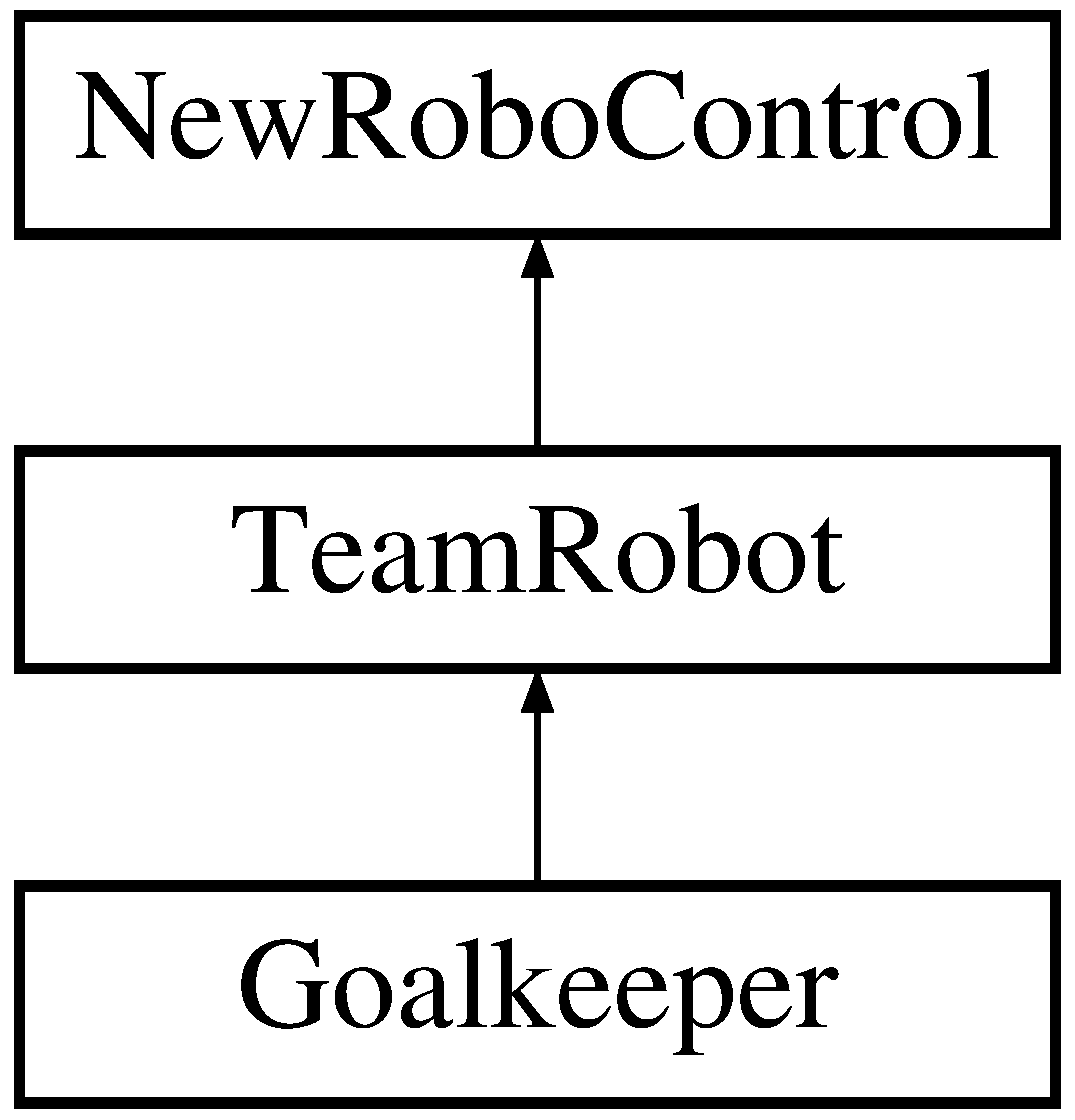
\includegraphics[height=3cm]{classGoalkeeper}
\end{center}
\end{figure}
\subsection*{Public Types}
\begin{DoxyCompactItemize}
\item 
enum \hyperlink{classGoalkeeper_a25db0bed632b4bdb87532b0fbbf45855}{ActionGk} \{ \hyperlink{classGoalkeeper_a25db0bed632b4bdb87532b0fbbf45855af1fa8ff07676a5e27f9cc78f6811c704}{GO\_\-TO\_\-DEF\_\-POS}, 
\hyperlink{classGoalkeeper_a25db0bed632b4bdb87532b0fbbf45855a96b7bc8aa3f3a4d1b68955f8d757e9c1}{PREVENT\_\-GOAL}, 
\hyperlink{classGoalkeeper_a25db0bed632b4bdb87532b0fbbf45855a7940a4d0074c5f5bb33743797387c2c1}{STOP}
 \}
\end{DoxyCompactItemize}
\subsection*{Public Member Functions}
\begin{DoxyCompactItemize}
\item 
\hyperlink{classGoalkeeper_a7ad214162340c37a695ba00d4576c3c4}{Goalkeeper} (RTDBConn \&DBC, const int deviceNr, const \hyperlink{classCoordinatesCalibrer}{CoordinatesCalibrer} $\ast$coordCalib, RawBall $\ast$ball, \hyperlink{classBallMonitor}{BallMonitor} $\ast$ballgk)
\item 
void \hyperlink{classGoalkeeper_abc394351f7c0d552c6e96da422c772ec}{setNextCmd} (const \hyperlink{structInterpreter_1_1GameData}{Interpreter::GameData} \&info)
\item 
void \hyperlink{classGoalkeeper_acfa6fbad0f6b1627fd59cc7cce6ff321}{setCmdParam} (const \hyperlink{classInterpreter}{Interpreter} \&interpreter)
\item 
void \hyperlink{classGoalkeeper_ab850d0d2278730bebc5479f1a339a925}{performCmd} (const \hyperlink{structInterpreter_1_1GameData}{Interpreter::GameData} \&info)
\end{DoxyCompactItemize}
\subsection*{Private Member Functions}
\begin{DoxyCompactItemize}
\item 
void \hyperlink{classGoalkeeper_a5287a2e74795bbec8f0ead767655da5d}{AddObstacleForFormation} (const \hyperlink{structInterpreter_1_1GameData}{Interpreter::GameData} \&info)
\end{DoxyCompactItemize}
\subsection*{Private Attributes}
\begin{DoxyCompactItemize}
\item 
\hyperlink{classGoalkeeper_a25db0bed632b4bdb87532b0fbbf45855}{ActionGk} \hyperlink{classGoalkeeper_a84e9e9f514d0ace81c95e03ee832aea8}{m\_\-nextCmd}
\item 
Position \hyperlink{classGoalkeeper_a04b3ca2b51698e36928ccce7569842eb}{m\_\-preventGoalParam}
\item 
\hyperlink{classBallMonitor}{BallMonitor} $\ast$ \hyperlink{classGoalkeeper_a8fc8e75ffc8d3582d293b0fe42a0c073}{m\_\-ballgk}
\end{DoxyCompactItemize}


\subsection{Member Enumeration Documentation}
\hypertarget{classGoalkeeper_a25db0bed632b4bdb87532b0fbbf45855}{
\index{Goalkeeper@{Goalkeeper}!ActionGk@{ActionGk}}
\index{ActionGk@{ActionGk}!Goalkeeper@{Goalkeeper}}
\subsubsection[{ActionGk}]{\setlength{\rightskip}{0pt plus 5cm}enum {\bf Goalkeeper::ActionGk}}}
\label{classGoalkeeper_a25db0bed632b4bdb87532b0fbbf45855}
\begin{Desc}
\item[Enumerator: ]\par
\begin{description}
\index{GO\_\-TO\_\-DEF\_\-POS@{GO\_\-TO\_\-DEF\_\-POS}!Goalkeeper@{Goalkeeper}}\index{Goalkeeper@{Goalkeeper}!GO\_\-TO\_\-DEF\_\-POS@{GO\_\-TO\_\-DEF\_\-POS}}\item[{\em 
\hypertarget{classGoalkeeper_a25db0bed632b4bdb87532b0fbbf45855af1fa8ff07676a5e27f9cc78f6811c704}{
GO\_\-TO\_\-DEF\_\-POS}
\label{classGoalkeeper_a25db0bed632b4bdb87532b0fbbf45855af1fa8ff07676a5e27f9cc78f6811c704}
}]TODO \index{PREVENT\_\-GOAL@{PREVENT\_\-GOAL}!Goalkeeper@{Goalkeeper}}\index{Goalkeeper@{Goalkeeper}!PREVENT\_\-GOAL@{PREVENT\_\-GOAL}}\item[{\em 
\hypertarget{classGoalkeeper_a25db0bed632b4bdb87532b0fbbf45855a96b7bc8aa3f3a4d1b68955f8d757e9c1}{
PREVENT\_\-GOAL}
\label{classGoalkeeper_a25db0bed632b4bdb87532b0fbbf45855a96b7bc8aa3f3a4d1b68955f8d757e9c1}
}]TODO \index{STOP@{STOP}!Goalkeeper@{Goalkeeper}}\index{Goalkeeper@{Goalkeeper}!STOP@{STOP}}\item[{\em 
\hypertarget{classGoalkeeper_a25db0bed632b4bdb87532b0fbbf45855a7940a4d0074c5f5bb33743797387c2c1}{
STOP}
\label{classGoalkeeper_a25db0bed632b4bdb87532b0fbbf45855a7940a4d0074c5f5bb33743797387c2c1}
}]TODO \end{description}
\end{Desc}



\subsection{Constructor \& Destructor Documentation}
\hypertarget{classGoalkeeper_a7ad214162340c37a695ba00d4576c3c4}{
\index{Goalkeeper@{Goalkeeper}!Goalkeeper@{Goalkeeper}}
\index{Goalkeeper@{Goalkeeper}!Goalkeeper@{Goalkeeper}}
\subsubsection[{Goalkeeper}]{\setlength{\rightskip}{0pt plus 5cm}Goalkeeper::Goalkeeper (RTDBConn \& {\em DBC}, \/  const int {\em deviceNr}, \/  const {\bf CoordinatesCalibrer} $\ast$ {\em coordCalib}, \/  RawBall $\ast$ {\em b}, \/  {\bf BallMonitor} $\ast$ {\em ballPm})}}
\label{classGoalkeeper_a7ad214162340c37a695ba00d4576c3c4}

\begin{DoxyParams}{Parameters}
\item[{\em DBC}]\item[{\em deviceNr}]\item[{\em coordCalib}]\item[{\em b}]\item[{\em ballPm}]\end{DoxyParams}


\subsection{Member Function Documentation}
\hypertarget{classGoalkeeper_a5287a2e74795bbec8f0ead767655da5d}{
\index{Goalkeeper@{Goalkeeper}!AddObstacleForFormation@{AddObstacleForFormation}}
\index{AddObstacleForFormation@{AddObstacleForFormation}!Goalkeeper@{Goalkeeper}}
\subsubsection[{AddObstacleForFormation}]{\setlength{\rightskip}{0pt plus 5cm}void Goalkeeper::AddObstacleForFormation (const {\bf Interpreter::GameData} \& {\em info})\hspace{0.3cm}{\ttfamily  \mbox{[}private, virtual\mbox{]}}}}
\label{classGoalkeeper_a5287a2e74795bbec8f0ead767655da5d}

\begin{DoxyParams}{Parameters}
\item[{\em info}]\end{DoxyParams}


Implements \hyperlink{classTeamRobot_a71ec65db46db1ac511fe17b668d4f192}{TeamRobot}.

\hypertarget{classGoalkeeper_ab850d0d2278730bebc5479f1a339a925}{
\index{Goalkeeper@{Goalkeeper}!performCmd@{performCmd}}
\index{performCmd@{performCmd}!Goalkeeper@{Goalkeeper}}
\subsubsection[{performCmd}]{\setlength{\rightskip}{0pt plus 5cm}void Goalkeeper::performCmd (const {\bf Interpreter::GameData} \& {\em info})\hspace{0.3cm}{\ttfamily  \mbox{[}virtual\mbox{]}}}}
\label{classGoalkeeper_ab850d0d2278730bebc5479f1a339a925}

\begin{DoxyParams}{Parameters}
\item[{\em info}]\end{DoxyParams}


Implements \hyperlink{classTeamRobot_a9b84df51ca16a7203fdb6498ea6741da}{TeamRobot}.

\hypertarget{classGoalkeeper_acfa6fbad0f6b1627fd59cc7cce6ff321}{
\index{Goalkeeper@{Goalkeeper}!setCmdParam@{setCmdParam}}
\index{setCmdParam@{setCmdParam}!Goalkeeper@{Goalkeeper}}
\subsubsection[{setCmdParam}]{\setlength{\rightskip}{0pt plus 5cm}void Goalkeeper::setCmdParam (const {\bf Interpreter} \& {\em interpreter})\hspace{0.3cm}{\ttfamily  \mbox{[}virtual\mbox{]}}}}
\label{classGoalkeeper_acfa6fbad0f6b1627fd59cc7cce6ff321}

\begin{DoxyParams}{Parameters}
\item[{\em interpreter}]\end{DoxyParams}


Implements \hyperlink{classTeamRobot_a34c0fd6986c510d4025e5752b3c0e49a}{TeamRobot}.

\hypertarget{classGoalkeeper_abc394351f7c0d552c6e96da422c772ec}{
\index{Goalkeeper@{Goalkeeper}!setNextCmd@{setNextCmd}}
\index{setNextCmd@{setNextCmd}!Goalkeeper@{Goalkeeper}}
\subsubsection[{setNextCmd}]{\setlength{\rightskip}{0pt plus 5cm}void Goalkeeper::setNextCmd (const {\bf Interpreter::GameData} \& {\em info})\hspace{0.3cm}{\ttfamily  \mbox{[}virtual\mbox{]}}}}
\label{classGoalkeeper_abc394351f7c0d552c6e96da422c772ec}

\begin{DoxyParams}{Parameters}
\item[{\em info}]\end{DoxyParams}


Implements \hyperlink{classTeamRobot_a65f9a2b7464dfac3f4a0336810cf574f}{TeamRobot}.



\subsection{Member Data Documentation}
\hypertarget{classGoalkeeper_a8fc8e75ffc8d3582d293b0fe42a0c073}{
\index{Goalkeeper@{Goalkeeper}!m\_\-ballgk@{m\_\-ballgk}}
\index{m\_\-ballgk@{m\_\-ballgk}!Goalkeeper@{Goalkeeper}}
\subsubsection[{m\_\-ballgk}]{\setlength{\rightskip}{0pt plus 5cm}{\bf BallMonitor}$\ast$ {\bf Goalkeeper::m\_\-ballgk}\hspace{0.3cm}{\ttfamily  \mbox{[}private\mbox{]}}}}
\label{classGoalkeeper_a8fc8e75ffc8d3582d293b0fe42a0c073}
TODO \hypertarget{classGoalkeeper_a84e9e9f514d0ace81c95e03ee832aea8}{
\index{Goalkeeper@{Goalkeeper}!m\_\-nextCmd@{m\_\-nextCmd}}
\index{m\_\-nextCmd@{m\_\-nextCmd}!Goalkeeper@{Goalkeeper}}
\subsubsection[{m\_\-nextCmd}]{\setlength{\rightskip}{0pt plus 5cm}{\bf ActionGk} {\bf Goalkeeper::m\_\-nextCmd}\hspace{0.3cm}{\ttfamily  \mbox{[}private\mbox{]}}}}
\label{classGoalkeeper_a84e9e9f514d0ace81c95e03ee832aea8}
TODO \hypertarget{classGoalkeeper_a04b3ca2b51698e36928ccce7569842eb}{
\index{Goalkeeper@{Goalkeeper}!m\_\-preventGoalParam@{m\_\-preventGoalParam}}
\index{m\_\-preventGoalParam@{m\_\-preventGoalParam}!Goalkeeper@{Goalkeeper}}
\subsubsection[{m\_\-preventGoalParam}]{\setlength{\rightskip}{0pt plus 5cm}Position {\bf Goalkeeper::m\_\-preventGoalParam}\hspace{0.3cm}{\ttfamily  \mbox{[}private\mbox{]}}}}
\label{classGoalkeeper_a04b3ca2b51698e36928ccce7569842eb}
TODO 

The documentation for this class was generated from the following files:\begin{DoxyCompactItemize}
\item 
src/\hyperlink{goalkeeper_8h}{goalkeeper.h}\item 
src/\hyperlink{goalkeeper_8cpp}{goalkeeper.cpp}\end{DoxyCompactItemize}

\hypertarget{classInterpreter}{
\section{Interpreter Class Reference}
\label{classInterpreter}\index{Interpreter@{Interpreter}}
}


Class used to coordinates actions and strategies for all robots from a high level point of view.  




{\ttfamily \#include $<$interpreter.h$>$}

\subsection*{Classes}
\begin{DoxyCompactItemize}
\item 
struct \hyperlink{structInterpreter_1_1GameData}{GameData}
\begin{DoxyCompactList}\small\item\em Structure to gather data about the current game. \item\end{DoxyCompactList}\item 
struct \hyperlink{structInterpreter_1_1Point}{Point}
\end{DoxyCompactItemize}
\subsection*{Public Types}
\begin{DoxyCompactItemize}
\item 
enum \hyperlink{classInterpreter_ac7c3ba77d973ffbb84b12db662cfe643}{KickTurn} \{ \hyperlink{classInterpreter_ac7c3ba77d973ffbb84b12db662cfe643a8c18a3c8b220a0c8166c1ee4b3504ebe}{OUR\_\-TURN}, 
\hyperlink{classInterpreter_ac7c3ba77d973ffbb84b12db662cfe643ac196847925fbe4bc38ee72b9b97d0f76}{THEIR\_\-TURN}
 \}
\begin{DoxyCompactList}\small\item\em Enum to describe the team having the Kick off / Penalty shooting. \item\end{DoxyCompactList}\item 
enum \hyperlink{classInterpreter_a0fb49436c8c14ca79e13f1cd78119088}{Strategy} \{ \hyperlink{classInterpreter_a0fb49436c8c14ca79e13f1cd78119088af1c3928f408be0d85ce73e1686e519d9}{INIT}, 
\hyperlink{classInterpreter_a0fb49436c8c14ca79e13f1cd78119088a8bf993c8b673e31f609171552d65c4c4}{ATK}, 
\hyperlink{classInterpreter_a0fb49436c8c14ca79e13f1cd78119088ae58df17fd988314c295b980f6a5a6a75}{DEF}, 
\hyperlink{classInterpreter_a0fb49436c8c14ca79e13f1cd78119088a5509091a7f3746995da83c92dd449187}{MIX}
 \}
\begin{DoxyCompactList}\small\item\em Enumeration of the possible playing strategies. \item\end{DoxyCompactList}\item 
typedef \hyperlink{classMatrix}{Matrix} \hyperlink{classInterpreter_a4c080f069f557cf92dfe803117a6ea53}{Map}
\end{DoxyCompactItemize}
\subsection*{Public Member Functions}
\begin{DoxyCompactItemize}
\item 
\hyperlink{classInterpreter_aa43e2d0df9f986ef4bde498aa8eadc04}{Interpreter} (eTeam x, Referee $\ast$y, \hyperlink{classGoalkeeper}{Goalkeeper} $\ast$z, \hyperlink{classPlayerMain}{PlayerMain} $\ast$p, \hyperlink{classPlayerTwo}{PlayerTwo} $\ast$t, \hyperlink{classOpponentRobot}{OpponentRobot} $\ast$a, \hyperlink{classOpponentRobot}{OpponentRobot} $\ast$b, \hyperlink{classOpponentRobot}{OpponentRobot} $\ast$c, RawBall $\ast$d, \hyperlink{classCoordinatesCalibrer}{CoordinatesCalibrer} $\ast$e)
\item 
\hyperlink{classInterpreter_a0f96b57f8126e2b5bc63390121e4b5b1}{$\sim$Interpreter} ()
\item 
void \hyperlink{classInterpreter_aa7c368c159002202e99b2c8b47acc534}{End} ()
\item 
\hyperlink{structInterpreter_1_1GameData}{GameData} \hyperlink{classInterpreter_adc77ada1a3d69c5e6bdfb2f1cc1a2e75}{getMode} () const 
\item 
void \hyperlink{classInterpreter_a4e5fcbc3020f3acd2d6855d12f8fe177}{SetP1MapToRobot} (\hyperlink{classTeamRobot}{TeamRobot} $\ast$p1) const 
\item 
void \hyperlink{classInterpreter_a3b96d97873572447193d3defe1bb877e}{SetP2MapToRobot} (\hyperlink{classTeamRobot}{TeamRobot} $\ast$p2) const 
\item 
Position \hyperlink{classInterpreter_aa8430187c89dffc8a9290d48ddd82346}{getGKDefaultPos} () const 
\item 
Position \hyperlink{classInterpreter_a2b46c460756f87d2dcef4ea8d8d49aaa}{getP1DefaultPos} () const 
\item 
Position \hyperlink{classInterpreter_ade297117d2ee20f524dd184ddd152c6d}{getP2DefaultPos} () const 
\item 
const \hyperlink{classGoalkeeper}{Goalkeeper} $\ast$ \hyperlink{classInterpreter_ac086d0ece936720419817ec19ebc3d8d}{getGK} () const 
\item 
const \hyperlink{classPlayerMain}{PlayerMain} $\ast$ \hyperlink{classInterpreter_af0d9f49ed686092925b626d032b0d9a6}{getP1} () const 
\item 
const \hyperlink{classPlayerTwo}{PlayerTwo} $\ast$ \hyperlink{classInterpreter_aa34b7799a25a0174b82690d09ce065f1}{getP2} () const 
\item 
const \hyperlink{classOpponentRobot}{OpponentRobot} $\ast$ \hyperlink{classInterpreter_acf9d8aba6db6063eb28e290ae1d4b655}{getE1} () const 
\item 
const \hyperlink{classOpponentRobot}{OpponentRobot} $\ast$ \hyperlink{classInterpreter_a46195d271e54a0e832876364562e4925}{getE2} () const 
\item 
const \hyperlink{classOpponentRobot}{OpponentRobot} $\ast$ \hyperlink{classInterpreter_a71c179ef0fa2c3372733dcae42799da3}{getE3} () const 
\item 
void \hyperlink{classInterpreter_a9b1dfdf67300251fb2c22f37e1d4c646}{updateSituation} ()
\item 
int \hyperlink{classInterpreter_ae09dee3df8e85f0d6b75b6dab5926850}{waitForUpdate} (int id)
\end{DoxyCompactItemize}
\subsection*{Static Public Member Functions}
\begin{DoxyCompactItemize}
\item 
static string \hyperlink{classInterpreter_a253118e59d7428286ff70a818efe0c52}{pathFind} (\hyperlink{classMatrix}{Map} map, \hyperlink{structInterpreter_1_1Point}{Point} start, \hyperlink{structInterpreter_1_1Point}{Point} finish)
\item 
static \hyperlink{structInterpreter_1_1Point}{Point} $\ast$ \hyperlink{classInterpreter_a17b252478116fc19ab8fe4623728cda8}{getCheckPoints} (\hyperlink{structInterpreter_1_1Point}{Point} start, string path)
\item 
static int \hyperlink{classInterpreter_a36e1b3f28a3d8dae2155f1f0212bed7d}{coord2mapX} (double)
\begin{DoxyCompactList}\small\item\em normalize the matrix to the real map \item\end{DoxyCompactList}\item 
static int \hyperlink{classInterpreter_a5b597351a6bdaf23fbf42aed910b151f}{coord2mapY} (double)
\item 
static double \hyperlink{classInterpreter_afaaf3930191f9ba3e48a09af193e0a39}{map2coordX} (int)
\begin{DoxyCompactList}\small\item\em normalize the matrix value to real map, or otherwise. \item\end{DoxyCompactList}\item 
static double \hyperlink{classInterpreter_abd0885c42ade8eb7f941c8d4b26a2501}{map2coordY} (int)
\begin{DoxyCompactList}\small\item\em normalize the matrix value to real map, or otherwise. \item\end{DoxyCompactList}\item 
static void \hyperlink{classInterpreter_a28fca7f91931cc48a0dc91cbbb08ba7a}{showMap} (const \hyperlink{classMatrix}{Map} \&map0, string path, \hyperlink{structInterpreter_1_1Point}{Point} start)
\item 
static void \hyperlink{classInterpreter_a4b195c13b5189f82d5b2ccd47ee4c562}{matrixupdate} (\hyperlink{classMatrix}{Map} \&map, const \hyperlink{classNewRoboControl}{NewRoboControl} $\ast$ref, const \hyperlink{classNewRoboControl}{NewRoboControl} $\ast$obstacles\mbox{[}5\mbox{]}, RawBall $\ast$ball, \hyperlink{classCoordinatesCalibrer}{CoordinatesCalibrer} $\ast$coordCalibrer, eSide our\_\-side)
\item 
static void \hyperlink{classInterpreter_a5bafd4ac63cb3dee9a6ddff172a0df02}{maskLowerRight} (\hyperlink{classMatrix}{Map} \&map)
\begin{DoxyCompactList}\small\item\em mix mode with overlap \item\end{DoxyCompactList}\item 
static void \hyperlink{classInterpreter_af02271dded17efbe47316706aad115f7}{maskLowerLeft} (\hyperlink{classMatrix}{Map} \&map)
\item 
static void \hyperlink{classInterpreter_a6741607033424bb90e95e59311941ed3}{maskUpperRight} (\hyperlink{classMatrix}{Map} \&map)
\item 
static void \hyperlink{classInterpreter_a1892fcf6bef01aa68c015c5a4a0c5f96}{maskUpperLeft} (\hyperlink{classMatrix}{Map} \&map)
\item 
static void \hyperlink{classInterpreter_a5aab0968d1a9c62fd20e1f11446deb73}{maskOmitLowerRight} (\hyperlink{classMatrix}{Map} \&map)
\item 
static void \hyperlink{classInterpreter_a849719043f4eef44634a9b5eb3e3561e}{maskOmitLowerLeft} (\hyperlink{classMatrix}{Map} \&map)
\item 
static void \hyperlink{classInterpreter_a83c078f3465a96026dbbc1ef3d7d120b}{maskOmitUpperRight} (\hyperlink{classMatrix}{Map} \&map)
\item 
static void \hyperlink{classInterpreter_a6232cdb6a8637bac127df9d19e8fd705}{maskOmitUpperLeft} (\hyperlink{classMatrix}{Map} \&map)
\item 
static void \hyperlink{classInterpreter_a454e31b3c1d0640be317c82c8b1b659d}{maskLeft} (\hyperlink{classMatrix}{Map} \&map)
\item 
static void \hyperlink{classInterpreter_abdfaacb7134b907d16a412ec1f80364b}{maskRight} (\hyperlink{classMatrix}{Map} \&map)
\end{DoxyCompactItemize}
\subsection*{Static Public Attributes}
\begin{DoxyCompactItemize}
\item 
static const double \hyperlink{classInterpreter_ad1c3ae1b11b176d50b5e8dcbf4b8b09e}{MID\_\-THRESHOLD} = 0.30
\item 
static const int \hyperlink{classInterpreter_a30c4dceff341b5e7cd36fdaba21aeaa9}{MAP\_\-WIDTH} = 100
\item 
static const int \hyperlink{classInterpreter_abda6b21064d50acd844bda3ed551e263}{MAP\_\-HEIGHT} = 80
\item 
static const int \hyperlink{classInterpreter_a0e360d1c91a1328af41fd9a4ede5eaef}{MAP\_\-BORDERSIZE} = 5
\item 
static const int \hyperlink{classInterpreter_a13a73024c4a1e62845a91f686adcd919}{DIR} = 8
\item 
static const int \hyperlink{classInterpreter_ac3d8a1b37737331fbfe7f4cea33cbd04}{DX} \mbox{[}\hyperlink{classInterpreter_a13a73024c4a1e62845a91f686adcd919}{DIR}\mbox{]} = \{1, 1, 0, -\/1, -\/1, -\/1, 0, 1\}
\item 
static const int \hyperlink{classInterpreter_aafc38675c9cad6e87686598dfe9c5758}{DY} \mbox{[}\hyperlink{classInterpreter_a13a73024c4a1e62845a91f686adcd919}{DIR}\mbox{]} = \{0, 1, 1, 1, 0, -\/1, -\/1, -\/1\}
\end{DoxyCompactItemize}
\subsection*{Private Member Functions}
\begin{DoxyCompactItemize}
\item 
void \hyperlink{classInterpreter_aef305fb79ee56df26f7fa4d2fb1be84e}{setPlayMode} ()
\item 
void \hyperlink{classInterpreter_a7bcbe98cfcb820392776af34325af2f4}{setSide} ()
\item 
void \hyperlink{classInterpreter_a976750d75dbde52f1de42b189bc3db0d}{setTurn} ()
\item 
void \hyperlink{classInterpreter_ad947f5a13997ba025515d65be4ca13a3}{setScores} ()
\item 
bool \hyperlink{classInterpreter_af8a7d8d22248eefd43de2ea08fc61b0f}{verifyPos} ()
\item 
void \hyperlink{classInterpreter_aa64d5e94c2cdee7696135a360f51926b}{setDefaultPos} ()
\item 
void \hyperlink{classInterpreter_a0191e3c65605b0ebadb696cf540951ee}{formationUpdateP1} ()
\item 
void \hyperlink{classInterpreter_aa722fe96daeb04f61352559e6d29dda6}{formationUpdateP2} ()
\end{DoxyCompactItemize}
\subsection*{Private Attributes}
\begin{DoxyCompactItemize}
\item 
\hyperlink{classCoordinatesCalibrer}{CoordinatesCalibrer} $\ast$ \hyperlink{classInterpreter_a734c73b13d471eb10d9a0ce772ffd906}{m\_\-cal}
\item 
Referee $\ast$ \hyperlink{classInterpreter_a883b74196b1cf25fc6461642c62bc4ec}{m\_\-ref}
\item 
const \hyperlink{classGoalkeeper}{Goalkeeper} $\ast$ \hyperlink{classInterpreter_a5c100f5098dbea4f12c8e65524914891}{m\_\-gk}
\item 
const \hyperlink{classPlayerMain}{PlayerMain} $\ast$ \hyperlink{classInterpreter_af450bd472149d0832c48e5da0a21ac77}{m\_\-p1}
\item 
const \hyperlink{classPlayerTwo}{PlayerTwo} $\ast$ \hyperlink{classInterpreter_aefbda2bf4d390731938a93ff3e2bfaa6}{m\_\-p2}
\item 
RawBall $\ast$ \hyperlink{classInterpreter_abed4bfde044196ee1ed466bcc62efbd2}{m\_\-ball}
\item 
const \hyperlink{classOpponentRobot}{OpponentRobot} $\ast$ \hyperlink{classInterpreter_a373544ccef8dc7630108349b589cee3d}{m\_\-e1}
\item 
const \hyperlink{classOpponentRobot}{OpponentRobot} $\ast$ \hyperlink{classInterpreter_aa04c8b2059980f776ea43c6f5e8e734b}{m\_\-e2}
\item 
const \hyperlink{classOpponentRobot}{OpponentRobot} $\ast$ \hyperlink{classInterpreter_ab61a3f3a1896b2d0d886aadcd15d72c1}{m\_\-e3}
\item 
\hyperlink{structInterpreter_1_1GameData}{GameData} \hyperlink{classInterpreter_aea59ccd407d1cbe579827da6ef24c9a1}{m\_\-mode}
\item 
int \hyperlink{classInterpreter_abe055996cec8f18725f3efb89e7e6ecb}{m\_\-situationId}
\item 
Position \hyperlink{classInterpreter_a3406559374dd0b28b8d702e5ba03189b}{m\_\-gkDefaultPosition}
\item 
Position \hyperlink{classInterpreter_a681f0273945917ab4dabec7b400bf001}{m\_\-p1DefaultPosition}
\item 
Position \hyperlink{classInterpreter_a2eb14ab69e51a5bdd6e393ed86b2d687}{m\_\-p2DefaultPosition}
\item 
pthread\_\-mutex\_\-t \hyperlink{classInterpreter_a4b1e804ce863d4d017e4b697e61e4017}{m\_\-mutex}
\item 
pthread\_\-cond\_\-t \hyperlink{classInterpreter_a9239b5f00f922f05a3902538784f5777}{m\_\-cond}
\item 
\hyperlink{classMatrix}{Map} \hyperlink{classInterpreter_a4c923fac8d283ef70a03812fce74ef47}{m\_\-p1Map}
\item 
\hyperlink{classMatrix}{Map} \hyperlink{classInterpreter_a9704ad86fdf8eddecfe191d8540fb4ef}{m\_\-p2Map}
\item 
pthread\_\-mutex\_\-t \hyperlink{classInterpreter_a849d1195573a32632ae33cd7ecd4bec7}{m\_\-p1MapMutex}
\item 
pthread\_\-mutex\_\-t \hyperlink{classInterpreter_a76012913dbff07096d081b2380c2c7a8}{m\_\-p2MapMutex}
\end{DoxyCompactItemize}


\subsection{Detailed Description}
Class used to coordinates actions and strategies for all robots from a high level point of view. 

\subsection{Member Typedef Documentation}
\hypertarget{classInterpreter_a4c080f069f557cf92dfe803117a6ea53}{
\index{Interpreter@{Interpreter}!Map@{Map}}
\index{Map@{Map}!Interpreter@{Interpreter}}
\subsubsection[{Map}]{\setlength{\rightskip}{0pt plus 5cm}typedef {\bf Matrix} {\bf Interpreter::Map}}}
\label{classInterpreter_a4c080f069f557cf92dfe803117a6ea53}


\subsection{Member Enumeration Documentation}
\hypertarget{classInterpreter_ac7c3ba77d973ffbb84b12db662cfe643}{
\index{Interpreter@{Interpreter}!KickTurn@{KickTurn}}
\index{KickTurn@{KickTurn}!Interpreter@{Interpreter}}
\subsubsection[{KickTurn}]{\setlength{\rightskip}{0pt plus 5cm}enum {\bf Interpreter::KickTurn}}}
\label{classInterpreter_ac7c3ba77d973ffbb84b12db662cfe643}


Enum to describe the team having the Kick off / Penalty shooting. 

\begin{Desc}
\item[Enumerator: ]\par
\begin{description}
\index{OUR\_\-TURN@{OUR\_\-TURN}!Interpreter@{Interpreter}}\index{Interpreter@{Interpreter}!OUR\_\-TURN@{OUR\_\-TURN}}\item[{\em 
\hypertarget{classInterpreter_ac7c3ba77d973ffbb84b12db662cfe643a8c18a3c8b220a0c8166c1ee4b3504ebe}{
OUR\_\-TURN}
\label{classInterpreter_ac7c3ba77d973ffbb84b12db662cfe643a8c18a3c8b220a0c8166c1ee4b3504ebe}
}]We have the kick off / penalty shooting \index{THEIR\_\-TURN@{THEIR\_\-TURN}!Interpreter@{Interpreter}}\index{Interpreter@{Interpreter}!THEIR\_\-TURN@{THEIR\_\-TURN}}\item[{\em 
\hypertarget{classInterpreter_ac7c3ba77d973ffbb84b12db662cfe643ac196847925fbe4bc38ee72b9b97d0f76}{
THEIR\_\-TURN}
\label{classInterpreter_ac7c3ba77d973ffbb84b12db662cfe643ac196847925fbe4bc38ee72b9b97d0f76}
}]The other team has the kick off / penalty shooting \end{description}
\end{Desc}

\hypertarget{classInterpreter_a0fb49436c8c14ca79e13f1cd78119088}{
\index{Interpreter@{Interpreter}!Strategy@{Strategy}}
\index{Strategy@{Strategy}!Interpreter@{Interpreter}}
\subsubsection[{Strategy}]{\setlength{\rightskip}{0pt plus 5cm}enum {\bf Interpreter::Strategy}}}
\label{classInterpreter_a0fb49436c8c14ca79e13f1cd78119088}


Enumeration of the possible playing strategies. 

\begin{Desc}
\item[Enumerator: ]\par
\begin{description}
\index{INIT@{INIT}!Interpreter@{Interpreter}}\index{Interpreter@{Interpreter}!INIT@{INIT}}\item[{\em 
\hypertarget{classInterpreter_a0fb49436c8c14ca79e13f1cd78119088af1c3928f408be0d85ce73e1686e519d9}{
INIT}
\label{classInterpreter_a0fb49436c8c14ca79e13f1cd78119088af1c3928f408be0d85ce73e1686e519d9}
}]Initial -\/ used for the start of the programm, must not be used afterwards. \index{ATK@{ATK}!Interpreter@{Interpreter}}\index{Interpreter@{Interpreter}!ATK@{ATK}}\item[{\em 
\hypertarget{classInterpreter_a0fb49436c8c14ca79e13f1cd78119088a8bf993c8b673e31f609171552d65c4c4}{
ATK}
\label{classInterpreter_a0fb49436c8c14ca79e13f1cd78119088a8bf993c8b673e31f609171552d65c4c4}
}]Attacking strategy \index{DEF@{DEF}!Interpreter@{Interpreter}}\index{Interpreter@{Interpreter}!DEF@{DEF}}\item[{\em 
\hypertarget{classInterpreter_a0fb49436c8c14ca79e13f1cd78119088ae58df17fd988314c295b980f6a5a6a75}{
DEF}
\label{classInterpreter_a0fb49436c8c14ca79e13f1cd78119088ae58df17fd988314c295b980f6a5a6a75}
}]Defensive strategy \index{MIX@{MIX}!Interpreter@{Interpreter}}\index{Interpreter@{Interpreter}!MIX@{MIX}}\item[{\em 
\hypertarget{classInterpreter_a0fb49436c8c14ca79e13f1cd78119088a5509091a7f3746995da83c92dd449187}{
MIX}
\label{classInterpreter_a0fb49436c8c14ca79e13f1cd78119088a5509091a7f3746995da83c92dd449187}
}]Mixed strategy \end{description}
\end{Desc}



\subsection{Constructor \& Destructor Documentation}
\hypertarget{classInterpreter_aa43e2d0df9f986ef4bde498aa8eadc04}{
\index{Interpreter@{Interpreter}!Interpreter@{Interpreter}}
\index{Interpreter@{Interpreter}!Interpreter@{Interpreter}}
\subsubsection[{Interpreter}]{\setlength{\rightskip}{0pt plus 5cm}Interpreter::Interpreter (eTeam {\em x}, \/  Referee $\ast$ {\em y}, \/  {\bf Goalkeeper} $\ast$ {\em z}, \/  {\bf PlayerMain} $\ast$ {\em p}, \/  {\bf PlayerTwo} $\ast$ {\em t}, \/  {\bf OpponentRobot} $\ast$ {\em a}, \/  {\bf OpponentRobot} $\ast$ {\em b}, \/  {\bf OpponentRobot} $\ast$ {\em c}, \/  RawBall $\ast$ {\em d}, \/  {\bf CoordinatesCalibrer} $\ast$ {\em e})}}
\label{classInterpreter_aa43e2d0df9f986ef4bde498aa8eadc04}

\begin{DoxyParams}{Parameters}
\item[{\em x}]\item[{\em y}]\item[{\em z}]\item[{\em p}]\item[{\em t}]\item[{\em a}]\item[{\em b}]\item[{\em c}]\item[{\em d}]\item[{\em e}]\end{DoxyParams}
\hypertarget{classInterpreter_a0f96b57f8126e2b5bc63390121e4b5b1}{
\index{Interpreter@{Interpreter}!$\sim$Interpreter@{$\sim$Interpreter}}
\index{$\sim$Interpreter@{$\sim$Interpreter}!Interpreter@{Interpreter}}
\subsubsection[{$\sim$Interpreter}]{\setlength{\rightskip}{0pt plus 5cm}Interpreter::$\sim$Interpreter ()}}
\label{classInterpreter_a0f96b57f8126e2b5bc63390121e4b5b1}


\subsection{Member Function Documentation}
\hypertarget{classInterpreter_a36e1b3f28a3d8dae2155f1f0212bed7d}{
\index{Interpreter@{Interpreter}!coord2mapX@{coord2mapX}}
\index{coord2mapX@{coord2mapX}!Interpreter@{Interpreter}}
\subsubsection[{coord2mapX}]{\setlength{\rightskip}{0pt plus 5cm}int Interpreter::coord2mapX (double {\em x})\hspace{0.3cm}{\ttfamily  \mbox{[}static\mbox{]}}}}
\label{classInterpreter_a36e1b3f28a3d8dae2155f1f0212bed7d}


normalize the matrix to the real map 


\begin{DoxyParams}{Parameters}
\item[{\em x}]is x value of the real map \end{DoxyParams}
\begin{DoxyReturn}{Returns}
int 
\end{DoxyReturn}
\hypertarget{classInterpreter_a5b597351a6bdaf23fbf42aed910b151f}{
\index{Interpreter@{Interpreter}!coord2mapY@{coord2mapY}}
\index{coord2mapY@{coord2mapY}!Interpreter@{Interpreter}}
\subsubsection[{coord2mapY}]{\setlength{\rightskip}{0pt plus 5cm}int Interpreter::coord2mapY (double {\em y})\hspace{0.3cm}{\ttfamily  \mbox{[}static\mbox{]}}}}
\label{classInterpreter_a5b597351a6bdaf23fbf42aed910b151f}

\begin{DoxyParams}{Parameters}
\item[{\em y}]\end{DoxyParams}
\begin{DoxyReturn}{Returns}
int 
\end{DoxyReturn}
\hypertarget{classInterpreter_aa7c368c159002202e99b2c8b47acc534}{
\index{Interpreter@{Interpreter}!End@{End}}
\index{End@{End}!Interpreter@{Interpreter}}
\subsubsection[{End}]{\setlength{\rightskip}{0pt plus 5cm}void Interpreter::End ()}}
\label{classInterpreter_aa7c368c159002202e99b2c8b47acc534}
\hypertarget{classInterpreter_a0191e3c65605b0ebadb696cf540951ee}{
\index{Interpreter@{Interpreter}!formationUpdateP1@{formationUpdateP1}}
\index{formationUpdateP1@{formationUpdateP1}!Interpreter@{Interpreter}}
\subsubsection[{formationUpdateP1}]{\setlength{\rightskip}{0pt plus 5cm}void Interpreter::formationUpdateP1 ()\hspace{0.3cm}{\ttfamily  \mbox{[}private\mbox{]}}}}
\label{classInterpreter_a0191e3c65605b0ebadb696cf540951ee}
\hypertarget{classInterpreter_aa722fe96daeb04f61352559e6d29dda6}{
\index{Interpreter@{Interpreter}!formationUpdateP2@{formationUpdateP2}}
\index{formationUpdateP2@{formationUpdateP2}!Interpreter@{Interpreter}}
\subsubsection[{formationUpdateP2}]{\setlength{\rightskip}{0pt plus 5cm}void Interpreter::formationUpdateP2 ()\hspace{0.3cm}{\ttfamily  \mbox{[}private\mbox{]}}}}
\label{classInterpreter_aa722fe96daeb04f61352559e6d29dda6}
\hypertarget{classInterpreter_a17b252478116fc19ab8fe4623728cda8}{
\index{Interpreter@{Interpreter}!getCheckPoints@{getCheckPoints}}
\index{getCheckPoints@{getCheckPoints}!Interpreter@{Interpreter}}
\subsubsection[{getCheckPoints}]{\setlength{\rightskip}{0pt plus 5cm}{\bf Interpreter::Point} $\ast$ Interpreter::getCheckPoints ({\bf Interpreter::Point} {\em start}, \/  string {\em path})\hspace{0.3cm}{\ttfamily  \mbox{[}static\mbox{]}}}}
\label{classInterpreter_a17b252478116fc19ab8fe4623728cda8}

\begin{DoxyParams}{Parameters}
\item[{\em start}]\item[{\em path}]\end{DoxyParams}
\begin{DoxyReturn}{Returns}
\hyperlink{structInterpreter_1_1Point}{Interpreter::Point} $\ast$ 
\end{DoxyReturn}
\hypertarget{classInterpreter_acf9d8aba6db6063eb28e290ae1d4b655}{
\index{Interpreter@{Interpreter}!getE1@{getE1}}
\index{getE1@{getE1}!Interpreter@{Interpreter}}
\subsubsection[{getE1}]{\setlength{\rightskip}{0pt plus 5cm}const {\bf OpponentRobot} $\ast$ Interpreter::getE1 () const}}
\label{classInterpreter_acf9d8aba6db6063eb28e290ae1d4b655}
\begin{DoxyReturn}{Returns}
const \hyperlink{classOpponentRobot}{OpponentRobot} $\ast$ 
\end{DoxyReturn}
\hypertarget{classInterpreter_a46195d271e54a0e832876364562e4925}{
\index{Interpreter@{Interpreter}!getE2@{getE2}}
\index{getE2@{getE2}!Interpreter@{Interpreter}}
\subsubsection[{getE2}]{\setlength{\rightskip}{0pt plus 5cm}const {\bf OpponentRobot} $\ast$ Interpreter::getE2 () const}}
\label{classInterpreter_a46195d271e54a0e832876364562e4925}
\begin{DoxyReturn}{Returns}
const \hyperlink{classOpponentRobot}{OpponentRobot} $\ast$ 
\end{DoxyReturn}
\hypertarget{classInterpreter_a71c179ef0fa2c3372733dcae42799da3}{
\index{Interpreter@{Interpreter}!getE3@{getE3}}
\index{getE3@{getE3}!Interpreter@{Interpreter}}
\subsubsection[{getE3}]{\setlength{\rightskip}{0pt plus 5cm}const {\bf OpponentRobot} $\ast$ Interpreter::getE3 () const}}
\label{classInterpreter_a71c179ef0fa2c3372733dcae42799da3}
\begin{DoxyReturn}{Returns}
const \hyperlink{classOpponentRobot}{OpponentRobot} $\ast$ 
\end{DoxyReturn}
\hypertarget{classInterpreter_ac086d0ece936720419817ec19ebc3d8d}{
\index{Interpreter@{Interpreter}!getGK@{getGK}}
\index{getGK@{getGK}!Interpreter@{Interpreter}}
\subsubsection[{getGK}]{\setlength{\rightskip}{0pt plus 5cm}const {\bf Goalkeeper} $\ast$ Interpreter::getGK () const}}
\label{classInterpreter_ac086d0ece936720419817ec19ebc3d8d}
\begin{DoxyReturn}{Returns}
const \hyperlink{classGoalkeeper}{Goalkeeper} $\ast$ 
\end{DoxyReturn}
\hypertarget{classInterpreter_aa8430187c89dffc8a9290d48ddd82346}{
\index{Interpreter@{Interpreter}!getGKDefaultPos@{getGKDefaultPos}}
\index{getGKDefaultPos@{getGKDefaultPos}!Interpreter@{Interpreter}}
\subsubsection[{getGKDefaultPos}]{\setlength{\rightskip}{0pt plus 5cm}Position Interpreter::getGKDefaultPos () const}}
\label{classInterpreter_aa8430187c89dffc8a9290d48ddd82346}
\begin{DoxyReturn}{Returns}
Position 
\end{DoxyReturn}
\hypertarget{classInterpreter_adc77ada1a3d69c5e6bdfb2f1cc1a2e75}{
\index{Interpreter@{Interpreter}!getMode@{getMode}}
\index{getMode@{getMode}!Interpreter@{Interpreter}}
\subsubsection[{getMode}]{\setlength{\rightskip}{0pt plus 5cm}{\bf Interpreter::GameData} Interpreter::getMode () const}}
\label{classInterpreter_adc77ada1a3d69c5e6bdfb2f1cc1a2e75}
\begin{DoxyReturn}{Returns}
\hyperlink{structInterpreter_1_1GameData}{Interpreter::GameData} 
\end{DoxyReturn}
\hypertarget{classInterpreter_af0d9f49ed686092925b626d032b0d9a6}{
\index{Interpreter@{Interpreter}!getP1@{getP1}}
\index{getP1@{getP1}!Interpreter@{Interpreter}}
\subsubsection[{getP1}]{\setlength{\rightskip}{0pt plus 5cm}const {\bf PlayerMain} $\ast$ Interpreter::getP1 () const}}
\label{classInterpreter_af0d9f49ed686092925b626d032b0d9a6}
\begin{DoxyReturn}{Returns}
const \hyperlink{classPlayerMain}{PlayerMain} $\ast$ 
\end{DoxyReturn}
\hypertarget{classInterpreter_a2b46c460756f87d2dcef4ea8d8d49aaa}{
\index{Interpreter@{Interpreter}!getP1DefaultPos@{getP1DefaultPos}}
\index{getP1DefaultPos@{getP1DefaultPos}!Interpreter@{Interpreter}}
\subsubsection[{getP1DefaultPos}]{\setlength{\rightskip}{0pt plus 5cm}Position Interpreter::getP1DefaultPos () const}}
\label{classInterpreter_a2b46c460756f87d2dcef4ea8d8d49aaa}
\begin{DoxyReturn}{Returns}
Position 
\end{DoxyReturn}
\hypertarget{classInterpreter_aa34b7799a25a0174b82690d09ce065f1}{
\index{Interpreter@{Interpreter}!getP2@{getP2}}
\index{getP2@{getP2}!Interpreter@{Interpreter}}
\subsubsection[{getP2}]{\setlength{\rightskip}{0pt plus 5cm}const {\bf PlayerTwo} $\ast$ Interpreter::getP2 () const}}
\label{classInterpreter_aa34b7799a25a0174b82690d09ce065f1}
\begin{DoxyReturn}{Returns}
const \hyperlink{classPlayerTwo}{PlayerTwo} $\ast$ 
\end{DoxyReturn}
\hypertarget{classInterpreter_ade297117d2ee20f524dd184ddd152c6d}{
\index{Interpreter@{Interpreter}!getP2DefaultPos@{getP2DefaultPos}}
\index{getP2DefaultPos@{getP2DefaultPos}!Interpreter@{Interpreter}}
\subsubsection[{getP2DefaultPos}]{\setlength{\rightskip}{0pt plus 5cm}Position Interpreter::getP2DefaultPos () const}}
\label{classInterpreter_ade297117d2ee20f524dd184ddd152c6d}
\begin{DoxyReturn}{Returns}
Position 
\end{DoxyReturn}
\hypertarget{classInterpreter_afaaf3930191f9ba3e48a09af193e0a39}{
\index{Interpreter@{Interpreter}!map2coordX@{map2coordX}}
\index{map2coordX@{map2coordX}!Interpreter@{Interpreter}}
\subsubsection[{map2coordX}]{\setlength{\rightskip}{0pt plus 5cm}double Interpreter::map2coordX (int {\em mapX})\hspace{0.3cm}{\ttfamily  \mbox{[}static\mbox{]}}}}
\label{classInterpreter_afaaf3930191f9ba3e48a09af193e0a39}


normalize the matrix value to real map, or otherwise. 


\begin{DoxyParams}{Parameters}
\item[{\em mapX}]\end{DoxyParams}
\begin{DoxyReturn}{Returns}
double 
\end{DoxyReturn}
\hypertarget{classInterpreter_abd0885c42ade8eb7f941c8d4b26a2501}{
\index{Interpreter@{Interpreter}!map2coordY@{map2coordY}}
\index{map2coordY@{map2coordY}!Interpreter@{Interpreter}}
\subsubsection[{map2coordY}]{\setlength{\rightskip}{0pt plus 5cm}double Interpreter::map2coordY (int {\em mapY})\hspace{0.3cm}{\ttfamily  \mbox{[}static\mbox{]}}}}
\label{classInterpreter_abd0885c42ade8eb7f941c8d4b26a2501}


normalize the matrix value to real map, or otherwise. 


\begin{DoxyParams}{Parameters}
\item[{\em mapY}]\end{DoxyParams}
\begin{DoxyReturn}{Returns}
double 
\end{DoxyReturn}
\hypertarget{classInterpreter_a454e31b3c1d0640be317c82c8b1b659d}{
\index{Interpreter@{Interpreter}!maskLeft@{maskLeft}}
\index{maskLeft@{maskLeft}!Interpreter@{Interpreter}}
\subsubsection[{maskLeft}]{\setlength{\rightskip}{0pt plus 5cm}void Interpreter::maskLeft ({\bf Map} \& {\em map})\hspace{0.3cm}{\ttfamily  \mbox{[}static\mbox{]}}}}
\label{classInterpreter_a454e31b3c1d0640be317c82c8b1b659d}

\begin{DoxyParams}{Parameters}
\item[{\em map}]\end{DoxyParams}
\hypertarget{classInterpreter_af02271dded17efbe47316706aad115f7}{
\index{Interpreter@{Interpreter}!maskLowerLeft@{maskLowerLeft}}
\index{maskLowerLeft@{maskLowerLeft}!Interpreter@{Interpreter}}
\subsubsection[{maskLowerLeft}]{\setlength{\rightskip}{0pt plus 5cm}void Interpreter::maskLowerLeft ({\bf Map} \& {\em map})\hspace{0.3cm}{\ttfamily  \mbox{[}static\mbox{]}}}}
\label{classInterpreter_af02271dded17efbe47316706aad115f7}

\begin{DoxyParams}{Parameters}
\item[{\em map}]\end{DoxyParams}
\hypertarget{classInterpreter_a5bafd4ac63cb3dee9a6ddff172a0df02}{
\index{Interpreter@{Interpreter}!maskLowerRight@{maskLowerRight}}
\index{maskLowerRight@{maskLowerRight}!Interpreter@{Interpreter}}
\subsubsection[{maskLowerRight}]{\setlength{\rightskip}{0pt plus 5cm}void Interpreter::maskLowerRight ({\bf Map} \& {\em map})\hspace{0.3cm}{\ttfamily  \mbox{[}static\mbox{]}}}}
\label{classInterpreter_a5bafd4ac63cb3dee9a6ddff172a0df02}


mix mode with overlap 


\begin{DoxyParams}{Parameters}
\item[{\em map}]\end{DoxyParams}
\hypertarget{classInterpreter_a849719043f4eef44634a9b5eb3e3561e}{
\index{Interpreter@{Interpreter}!maskOmitLowerLeft@{maskOmitLowerLeft}}
\index{maskOmitLowerLeft@{maskOmitLowerLeft}!Interpreter@{Interpreter}}
\subsubsection[{maskOmitLowerLeft}]{\setlength{\rightskip}{0pt plus 5cm}void Interpreter::maskOmitLowerLeft ({\bf Map} \& {\em map})\hspace{0.3cm}{\ttfamily  \mbox{[}static\mbox{]}}}}
\label{classInterpreter_a849719043f4eef44634a9b5eb3e3561e}

\begin{DoxyParams}{Parameters}
\item[{\em map}]\end{DoxyParams}
\hypertarget{classInterpreter_a5aab0968d1a9c62fd20e1f11446deb73}{
\index{Interpreter@{Interpreter}!maskOmitLowerRight@{maskOmitLowerRight}}
\index{maskOmitLowerRight@{maskOmitLowerRight}!Interpreter@{Interpreter}}
\subsubsection[{maskOmitLowerRight}]{\setlength{\rightskip}{0pt plus 5cm}void Interpreter::maskOmitLowerRight ({\bf Map} \& {\em map})\hspace{0.3cm}{\ttfamily  \mbox{[}static\mbox{]}}}}
\label{classInterpreter_a5aab0968d1a9c62fd20e1f11446deb73}

\begin{DoxyParams}{Parameters}
\item[{\em map}]\end{DoxyParams}
\hypertarget{classInterpreter_a6232cdb6a8637bac127df9d19e8fd705}{
\index{Interpreter@{Interpreter}!maskOmitUpperLeft@{maskOmitUpperLeft}}
\index{maskOmitUpperLeft@{maskOmitUpperLeft}!Interpreter@{Interpreter}}
\subsubsection[{maskOmitUpperLeft}]{\setlength{\rightskip}{0pt plus 5cm}void Interpreter::maskOmitUpperLeft ({\bf Map} \& {\em map})\hspace{0.3cm}{\ttfamily  \mbox{[}static\mbox{]}}}}
\label{classInterpreter_a6232cdb6a8637bac127df9d19e8fd705}

\begin{DoxyParams}{Parameters}
\item[{\em map}]\end{DoxyParams}
\hypertarget{classInterpreter_a83c078f3465a96026dbbc1ef3d7d120b}{
\index{Interpreter@{Interpreter}!maskOmitUpperRight@{maskOmitUpperRight}}
\index{maskOmitUpperRight@{maskOmitUpperRight}!Interpreter@{Interpreter}}
\subsubsection[{maskOmitUpperRight}]{\setlength{\rightskip}{0pt plus 5cm}void Interpreter::maskOmitUpperRight ({\bf Map} \& {\em map})\hspace{0.3cm}{\ttfamily  \mbox{[}static\mbox{]}}}}
\label{classInterpreter_a83c078f3465a96026dbbc1ef3d7d120b}

\begin{DoxyParams}{Parameters}
\item[{\em map}]\end{DoxyParams}
\hypertarget{classInterpreter_abdfaacb7134b907d16a412ec1f80364b}{
\index{Interpreter@{Interpreter}!maskRight@{maskRight}}
\index{maskRight@{maskRight}!Interpreter@{Interpreter}}
\subsubsection[{maskRight}]{\setlength{\rightskip}{0pt plus 5cm}void Interpreter::maskRight ({\bf Map} \& {\em map})\hspace{0.3cm}{\ttfamily  \mbox{[}static\mbox{]}}}}
\label{classInterpreter_abdfaacb7134b907d16a412ec1f80364b}

\begin{DoxyParams}{Parameters}
\item[{\em map}]\end{DoxyParams}
\hypertarget{classInterpreter_a1892fcf6bef01aa68c015c5a4a0c5f96}{
\index{Interpreter@{Interpreter}!maskUpperLeft@{maskUpperLeft}}
\index{maskUpperLeft@{maskUpperLeft}!Interpreter@{Interpreter}}
\subsubsection[{maskUpperLeft}]{\setlength{\rightskip}{0pt plus 5cm}void Interpreter::maskUpperLeft ({\bf Map} \& {\em map})\hspace{0.3cm}{\ttfamily  \mbox{[}static\mbox{]}}}}
\label{classInterpreter_a1892fcf6bef01aa68c015c5a4a0c5f96}

\begin{DoxyParams}{Parameters}
\item[{\em map}]\end{DoxyParams}
\hypertarget{classInterpreter_a6741607033424bb90e95e59311941ed3}{
\index{Interpreter@{Interpreter}!maskUpperRight@{maskUpperRight}}
\index{maskUpperRight@{maskUpperRight}!Interpreter@{Interpreter}}
\subsubsection[{maskUpperRight}]{\setlength{\rightskip}{0pt plus 5cm}void Interpreter::maskUpperRight ({\bf Map} \& {\em map})\hspace{0.3cm}{\ttfamily  \mbox{[}static\mbox{]}}}}
\label{classInterpreter_a6741607033424bb90e95e59311941ed3}

\begin{DoxyParams}{Parameters}
\item[{\em map}]\end{DoxyParams}
\hypertarget{classInterpreter_a4b195c13b5189f82d5b2ccd47ee4c562}{
\index{Interpreter@{Interpreter}!matrixupdate@{matrixupdate}}
\index{matrixupdate@{matrixupdate}!Interpreter@{Interpreter}}
\subsubsection[{matrixupdate}]{\setlength{\rightskip}{0pt plus 5cm}void Interpreter::matrixupdate ({\bf Interpreter::Map} \& {\em map}, \/  const {\bf NewRoboControl} $\ast$ {\em ref}, \/  const {\bf NewRoboControl} $\ast$ {\em obstacles}\mbox{[}5\mbox{]}, \/  RawBall $\ast$ {\em ball}, \/  {\bf CoordinatesCalibrer} $\ast$ {\em coordCalibrer}, \/  eSide {\em our\_\-side})\hspace{0.3cm}{\ttfamily  \mbox{[}static\mbox{]}}}}
\label{classInterpreter_a4b195c13b5189f82d5b2ccd47ee4c562}

\begin{DoxyParams}{Parameters}
\item[{\em map}]\item[{\em ref}]\item[{\em obstacles\mbox{[}$\,$\mbox{]}}]\item[{\em ball}]\item[{\em coordCalibrer}]\item[{\em our\_\-side}]\end{DoxyParams}
\hypertarget{classInterpreter_a253118e59d7428286ff70a818efe0c52}{
\index{Interpreter@{Interpreter}!pathFind@{pathFind}}
\index{pathFind@{pathFind}!Interpreter@{Interpreter}}
\subsubsection[{pathFind}]{\setlength{\rightskip}{0pt plus 5cm}string Interpreter::pathFind ({\bf Interpreter::Map} {\em map}, \/  {\bf Interpreter::Point} {\em start}, \/  {\bf Interpreter::Point} {\em finish})\hspace{0.3cm}{\ttfamily  \mbox{[}static\mbox{]}}}}
\label{classInterpreter_a253118e59d7428286ff70a818efe0c52}

\begin{DoxyParams}{Parameters}
\item[{\em map}]\item[{\em start}]\item[{\em finish}]\end{DoxyParams}
\begin{DoxyReturn}{Returns}
string 
\end{DoxyReturn}
\hypertarget{classInterpreter_aa64d5e94c2cdee7696135a360f51926b}{
\index{Interpreter@{Interpreter}!setDefaultPos@{setDefaultPos}}
\index{setDefaultPos@{setDefaultPos}!Interpreter@{Interpreter}}
\subsubsection[{setDefaultPos}]{\setlength{\rightskip}{0pt plus 5cm}void Interpreter::setDefaultPos ()\hspace{0.3cm}{\ttfamily  \mbox{[}private\mbox{]}}}}
\label{classInterpreter_aa64d5e94c2cdee7696135a360f51926b}
\hypertarget{classInterpreter_a4e5fcbc3020f3acd2d6855d12f8fe177}{
\index{Interpreter@{Interpreter}!SetP1MapToRobot@{SetP1MapToRobot}}
\index{SetP1MapToRobot@{SetP1MapToRobot}!Interpreter@{Interpreter}}
\subsubsection[{SetP1MapToRobot}]{\setlength{\rightskip}{0pt plus 5cm}void Interpreter::SetP1MapToRobot ({\bf TeamRobot} $\ast$ {\em p1}) const}}
\label{classInterpreter_a4e5fcbc3020f3acd2d6855d12f8fe177}

\begin{DoxyParams}{Parameters}
\item[{\em p1}]\end{DoxyParams}
\hypertarget{classInterpreter_a3b96d97873572447193d3defe1bb877e}{
\index{Interpreter@{Interpreter}!SetP2MapToRobot@{SetP2MapToRobot}}
\index{SetP2MapToRobot@{SetP2MapToRobot}!Interpreter@{Interpreter}}
\subsubsection[{SetP2MapToRobot}]{\setlength{\rightskip}{0pt plus 5cm}void Interpreter::SetP2MapToRobot ({\bf TeamRobot} $\ast$ {\em p2}) const}}
\label{classInterpreter_a3b96d97873572447193d3defe1bb877e}

\begin{DoxyParams}{Parameters}
\item[{\em p2}]\end{DoxyParams}
\hypertarget{classInterpreter_aef305fb79ee56df26f7fa4d2fb1be84e}{
\index{Interpreter@{Interpreter}!setPlayMode@{setPlayMode}}
\index{setPlayMode@{setPlayMode}!Interpreter@{Interpreter}}
\subsubsection[{setPlayMode}]{\setlength{\rightskip}{0pt plus 5cm}void Interpreter::setPlayMode ()\hspace{0.3cm}{\ttfamily  \mbox{[}private\mbox{]}}}}
\label{classInterpreter_aef305fb79ee56df26f7fa4d2fb1be84e}
\hypertarget{classInterpreter_ad947f5a13997ba025515d65be4ca13a3}{
\index{Interpreter@{Interpreter}!setScores@{setScores}}
\index{setScores@{setScores}!Interpreter@{Interpreter}}
\subsubsection[{setScores}]{\setlength{\rightskip}{0pt plus 5cm}void Interpreter::setScores ()\hspace{0.3cm}{\ttfamily  \mbox{[}private\mbox{]}}}}
\label{classInterpreter_ad947f5a13997ba025515d65be4ca13a3}
\hypertarget{classInterpreter_a7bcbe98cfcb820392776af34325af2f4}{
\index{Interpreter@{Interpreter}!setSide@{setSide}}
\index{setSide@{setSide}!Interpreter@{Interpreter}}
\subsubsection[{setSide}]{\setlength{\rightskip}{0pt plus 5cm}void Interpreter::setSide ()\hspace{0.3cm}{\ttfamily  \mbox{[}private\mbox{]}}}}
\label{classInterpreter_a7bcbe98cfcb820392776af34325af2f4}
\hypertarget{classInterpreter_a976750d75dbde52f1de42b189bc3db0d}{
\index{Interpreter@{Interpreter}!setTurn@{setTurn}}
\index{setTurn@{setTurn}!Interpreter@{Interpreter}}
\subsubsection[{setTurn}]{\setlength{\rightskip}{0pt plus 5cm}void Interpreter::setTurn ()\hspace{0.3cm}{\ttfamily  \mbox{[}private\mbox{]}}}}
\label{classInterpreter_a976750d75dbde52f1de42b189bc3db0d}
\hypertarget{classInterpreter_a28fca7f91931cc48a0dc91cbbb08ba7a}{
\index{Interpreter@{Interpreter}!showMap@{showMap}}
\index{showMap@{showMap}!Interpreter@{Interpreter}}
\subsubsection[{showMap}]{\setlength{\rightskip}{0pt plus 5cm}void Interpreter::showMap (const {\bf Map} \& {\em map0}, \/  string {\em path}, \/  {\bf Interpreter::Point} {\em start})\hspace{0.3cm}{\ttfamily  \mbox{[}static\mbox{]}}}}
\label{classInterpreter_a28fca7f91931cc48a0dc91cbbb08ba7a}

\begin{DoxyParams}{Parameters}
\item[{\em map0}]\item[{\em path}]\item[{\em start}]\end{DoxyParams}
\hypertarget{classInterpreter_a9b1dfdf67300251fb2c22f37e1d4c646}{
\index{Interpreter@{Interpreter}!updateSituation@{updateSituation}}
\index{updateSituation@{updateSituation}!Interpreter@{Interpreter}}
\subsubsection[{updateSituation}]{\setlength{\rightskip}{0pt plus 5cm}void Interpreter::updateSituation ()}}
\label{classInterpreter_a9b1dfdf67300251fb2c22f37e1d4c646}
\hypertarget{classInterpreter_af8a7d8d22248eefd43de2ea08fc61b0f}{
\index{Interpreter@{Interpreter}!verifyPos@{verifyPos}}
\index{verifyPos@{verifyPos}!Interpreter@{Interpreter}}
\subsubsection[{verifyPos}]{\setlength{\rightskip}{0pt plus 5cm}bool Interpreter::verifyPos ()\hspace{0.3cm}{\ttfamily  \mbox{[}private\mbox{]}}}}
\label{classInterpreter_af8a7d8d22248eefd43de2ea08fc61b0f}
\begin{DoxyReturn}{Returns}
bool 
\end{DoxyReturn}
\hypertarget{classInterpreter_ae09dee3df8e85f0d6b75b6dab5926850}{
\index{Interpreter@{Interpreter}!waitForUpdate@{waitForUpdate}}
\index{waitForUpdate@{waitForUpdate}!Interpreter@{Interpreter}}
\subsubsection[{waitForUpdate}]{\setlength{\rightskip}{0pt plus 5cm}int Interpreter::waitForUpdate (int {\em id})}}
\label{classInterpreter_ae09dee3df8e85f0d6b75b6dab5926850}

\begin{DoxyParams}{Parameters}
\item[{\em id}]\end{DoxyParams}
\begin{DoxyReturn}{Returns}
int 
\end{DoxyReturn}


\subsection{Member Data Documentation}
\hypertarget{classInterpreter_a13a73024c4a1e62845a91f686adcd919}{
\index{Interpreter@{Interpreter}!DIR@{DIR}}
\index{DIR@{DIR}!Interpreter@{Interpreter}}
\subsubsection[{DIR}]{\setlength{\rightskip}{0pt plus 5cm}const int {\bf Interpreter::DIR} = 8\hspace{0.3cm}{\ttfamily  \mbox{[}static\mbox{]}}}}
\label{classInterpreter_a13a73024c4a1e62845a91f686adcd919}
Number of possible directions to go at any position \hypertarget{classInterpreter_ac3d8a1b37737331fbfe7f4cea33cbd04}{
\index{Interpreter@{Interpreter}!DX@{DX}}
\index{DX@{DX}!Interpreter@{Interpreter}}
\subsubsection[{DX}]{\setlength{\rightskip}{0pt plus 5cm}const int {\bf Interpreter::DX} = \{1, 1, 0, -\/1, -\/1, -\/1, 0, 1\}\hspace{0.3cm}{\ttfamily  \mbox{[}static\mbox{]}}}}
\label{classInterpreter_ac3d8a1b37737331fbfe7f4cea33cbd04}
TODO \hypertarget{classInterpreter_aafc38675c9cad6e87686598dfe9c5758}{
\index{Interpreter@{Interpreter}!DY@{DY}}
\index{DY@{DY}!Interpreter@{Interpreter}}
\subsubsection[{DY}]{\setlength{\rightskip}{0pt plus 5cm}const int {\bf Interpreter::DY} = \{0, 1, 1, 1, 0, -\/1, -\/1, -\/1\}\hspace{0.3cm}{\ttfamily  \mbox{[}static\mbox{]}}}}
\label{classInterpreter_aafc38675c9cad6e87686598dfe9c5758}
TODO \hypertarget{classInterpreter_abed4bfde044196ee1ed466bcc62efbd2}{
\index{Interpreter@{Interpreter}!m\_\-ball@{m\_\-ball}}
\index{m\_\-ball@{m\_\-ball}!Interpreter@{Interpreter}}
\subsubsection[{m\_\-ball}]{\setlength{\rightskip}{0pt plus 5cm}RawBall$\ast$ {\bf Interpreter::m\_\-ball}\hspace{0.3cm}{\ttfamily  \mbox{[}private\mbox{]}}}}
\label{classInterpreter_abed4bfde044196ee1ed466bcc62efbd2}
TODO \hypertarget{classInterpreter_a734c73b13d471eb10d9a0ce772ffd906}{
\index{Interpreter@{Interpreter}!m\_\-cal@{m\_\-cal}}
\index{m\_\-cal@{m\_\-cal}!Interpreter@{Interpreter}}
\subsubsection[{m\_\-cal}]{\setlength{\rightskip}{0pt plus 5cm}{\bf CoordinatesCalibrer}$\ast$ {\bf Interpreter::m\_\-cal}\hspace{0.3cm}{\ttfamily  \mbox{[}private\mbox{]}}}}
\label{classInterpreter_a734c73b13d471eb10d9a0ce772ffd906}
TODO \hypertarget{classInterpreter_a9239b5f00f922f05a3902538784f5777}{
\index{Interpreter@{Interpreter}!m\_\-cond@{m\_\-cond}}
\index{m\_\-cond@{m\_\-cond}!Interpreter@{Interpreter}}
\subsubsection[{m\_\-cond}]{\setlength{\rightskip}{0pt plus 5cm}pthread\_\-cond\_\-t {\bf Interpreter::m\_\-cond}\hspace{0.3cm}{\ttfamily  \mbox{[}private\mbox{]}}}}
\label{classInterpreter_a9239b5f00f922f05a3902538784f5777}
TODO \hypertarget{classInterpreter_a373544ccef8dc7630108349b589cee3d}{
\index{Interpreter@{Interpreter}!m\_\-e1@{m\_\-e1}}
\index{m\_\-e1@{m\_\-e1}!Interpreter@{Interpreter}}
\subsubsection[{m\_\-e1}]{\setlength{\rightskip}{0pt plus 5cm}const {\bf OpponentRobot}$\ast$ {\bf Interpreter::m\_\-e1}\hspace{0.3cm}{\ttfamily  \mbox{[}private\mbox{]}}}}
\label{classInterpreter_a373544ccef8dc7630108349b589cee3d}
TODO \hypertarget{classInterpreter_aa04c8b2059980f776ea43c6f5e8e734b}{
\index{Interpreter@{Interpreter}!m\_\-e2@{m\_\-e2}}
\index{m\_\-e2@{m\_\-e2}!Interpreter@{Interpreter}}
\subsubsection[{m\_\-e2}]{\setlength{\rightskip}{0pt plus 5cm}const {\bf OpponentRobot}$\ast$ {\bf Interpreter::m\_\-e2}\hspace{0.3cm}{\ttfamily  \mbox{[}private\mbox{]}}}}
\label{classInterpreter_aa04c8b2059980f776ea43c6f5e8e734b}
TODO \hypertarget{classInterpreter_ab61a3f3a1896b2d0d886aadcd15d72c1}{
\index{Interpreter@{Interpreter}!m\_\-e3@{m\_\-e3}}
\index{m\_\-e3@{m\_\-e3}!Interpreter@{Interpreter}}
\subsubsection[{m\_\-e3}]{\setlength{\rightskip}{0pt plus 5cm}const {\bf OpponentRobot}$\ast$ {\bf Interpreter::m\_\-e3}\hspace{0.3cm}{\ttfamily  \mbox{[}private\mbox{]}}}}
\label{classInterpreter_ab61a3f3a1896b2d0d886aadcd15d72c1}
TODO \hypertarget{classInterpreter_a5c100f5098dbea4f12c8e65524914891}{
\index{Interpreter@{Interpreter}!m\_\-gk@{m\_\-gk}}
\index{m\_\-gk@{m\_\-gk}!Interpreter@{Interpreter}}
\subsubsection[{m\_\-gk}]{\setlength{\rightskip}{0pt plus 5cm}const {\bf Goalkeeper}$\ast$ {\bf Interpreter::m\_\-gk}\hspace{0.3cm}{\ttfamily  \mbox{[}private\mbox{]}}}}
\label{classInterpreter_a5c100f5098dbea4f12c8e65524914891}
TODO \hypertarget{classInterpreter_a3406559374dd0b28b8d702e5ba03189b}{
\index{Interpreter@{Interpreter}!m\_\-gkDefaultPosition@{m\_\-gkDefaultPosition}}
\index{m\_\-gkDefaultPosition@{m\_\-gkDefaultPosition}!Interpreter@{Interpreter}}
\subsubsection[{m\_\-gkDefaultPosition}]{\setlength{\rightskip}{0pt plus 5cm}Position {\bf Interpreter::m\_\-gkDefaultPosition}\hspace{0.3cm}{\ttfamily  \mbox{[}private\mbox{]}}}}
\label{classInterpreter_a3406559374dd0b28b8d702e5ba03189b}
TODO \hypertarget{classInterpreter_aea59ccd407d1cbe579827da6ef24c9a1}{
\index{Interpreter@{Interpreter}!m\_\-mode@{m\_\-mode}}
\index{m\_\-mode@{m\_\-mode}!Interpreter@{Interpreter}}
\subsubsection[{m\_\-mode}]{\setlength{\rightskip}{0pt plus 5cm}{\bf GameData} {\bf Interpreter::m\_\-mode}\hspace{0.3cm}{\ttfamily  \mbox{[}private\mbox{]}}}}
\label{classInterpreter_aea59ccd407d1cbe579827da6ef24c9a1}
TODO \hypertarget{classInterpreter_a4b1e804ce863d4d017e4b697e61e4017}{
\index{Interpreter@{Interpreter}!m\_\-mutex@{m\_\-mutex}}
\index{m\_\-mutex@{m\_\-mutex}!Interpreter@{Interpreter}}
\subsubsection[{m\_\-mutex}]{\setlength{\rightskip}{0pt plus 5cm}pthread\_\-mutex\_\-t {\bf Interpreter::m\_\-mutex}\hspace{0.3cm}{\ttfamily  \mbox{[}private\mbox{]}}}}
\label{classInterpreter_a4b1e804ce863d4d017e4b697e61e4017}
TODO \hypertarget{classInterpreter_af450bd472149d0832c48e5da0a21ac77}{
\index{Interpreter@{Interpreter}!m\_\-p1@{m\_\-p1}}
\index{m\_\-p1@{m\_\-p1}!Interpreter@{Interpreter}}
\subsubsection[{m\_\-p1}]{\setlength{\rightskip}{0pt plus 5cm}const {\bf PlayerMain}$\ast$ {\bf Interpreter::m\_\-p1}\hspace{0.3cm}{\ttfamily  \mbox{[}private\mbox{]}}}}
\label{classInterpreter_af450bd472149d0832c48e5da0a21ac77}
TODO \hypertarget{classInterpreter_a681f0273945917ab4dabec7b400bf001}{
\index{Interpreter@{Interpreter}!m\_\-p1DefaultPosition@{m\_\-p1DefaultPosition}}
\index{m\_\-p1DefaultPosition@{m\_\-p1DefaultPosition}!Interpreter@{Interpreter}}
\subsubsection[{m\_\-p1DefaultPosition}]{\setlength{\rightskip}{0pt plus 5cm}Position {\bf Interpreter::m\_\-p1DefaultPosition}\hspace{0.3cm}{\ttfamily  \mbox{[}private\mbox{]}}}}
\label{classInterpreter_a681f0273945917ab4dabec7b400bf001}
TODO \hypertarget{classInterpreter_a4c923fac8d283ef70a03812fce74ef47}{
\index{Interpreter@{Interpreter}!m\_\-p1Map@{m\_\-p1Map}}
\index{m\_\-p1Map@{m\_\-p1Map}!Interpreter@{Interpreter}}
\subsubsection[{m\_\-p1Map}]{\setlength{\rightskip}{0pt plus 5cm}{\bf Map} {\bf Interpreter::m\_\-p1Map}\hspace{0.3cm}{\ttfamily  \mbox{[}private\mbox{]}}}}
\label{classInterpreter_a4c923fac8d283ef70a03812fce74ef47}
TODO \hypertarget{classInterpreter_a849d1195573a32632ae33cd7ecd4bec7}{
\index{Interpreter@{Interpreter}!m\_\-p1MapMutex@{m\_\-p1MapMutex}}
\index{m\_\-p1MapMutex@{m\_\-p1MapMutex}!Interpreter@{Interpreter}}
\subsubsection[{m\_\-p1MapMutex}]{\setlength{\rightskip}{0pt plus 5cm}pthread\_\-mutex\_\-t {\bf Interpreter::m\_\-p1MapMutex}\hspace{0.3cm}{\ttfamily  \mbox{[}private\mbox{]}}}}
\label{classInterpreter_a849d1195573a32632ae33cd7ecd4bec7}
TODO \hypertarget{classInterpreter_aefbda2bf4d390731938a93ff3e2bfaa6}{
\index{Interpreter@{Interpreter}!m\_\-p2@{m\_\-p2}}
\index{m\_\-p2@{m\_\-p2}!Interpreter@{Interpreter}}
\subsubsection[{m\_\-p2}]{\setlength{\rightskip}{0pt plus 5cm}const {\bf PlayerTwo}$\ast$ {\bf Interpreter::m\_\-p2}\hspace{0.3cm}{\ttfamily  \mbox{[}private\mbox{]}}}}
\label{classInterpreter_aefbda2bf4d390731938a93ff3e2bfaa6}
TODO \hypertarget{classInterpreter_a2eb14ab69e51a5bdd6e393ed86b2d687}{
\index{Interpreter@{Interpreter}!m\_\-p2DefaultPosition@{m\_\-p2DefaultPosition}}
\index{m\_\-p2DefaultPosition@{m\_\-p2DefaultPosition}!Interpreter@{Interpreter}}
\subsubsection[{m\_\-p2DefaultPosition}]{\setlength{\rightskip}{0pt plus 5cm}Position {\bf Interpreter::m\_\-p2DefaultPosition}\hspace{0.3cm}{\ttfamily  \mbox{[}private\mbox{]}}}}
\label{classInterpreter_a2eb14ab69e51a5bdd6e393ed86b2d687}
TODO \hypertarget{classInterpreter_a9704ad86fdf8eddecfe191d8540fb4ef}{
\index{Interpreter@{Interpreter}!m\_\-p2Map@{m\_\-p2Map}}
\index{m\_\-p2Map@{m\_\-p2Map}!Interpreter@{Interpreter}}
\subsubsection[{m\_\-p2Map}]{\setlength{\rightskip}{0pt plus 5cm}{\bf Map} {\bf Interpreter::m\_\-p2Map}\hspace{0.3cm}{\ttfamily  \mbox{[}private\mbox{]}}}}
\label{classInterpreter_a9704ad86fdf8eddecfe191d8540fb4ef}
TODO \hypertarget{classInterpreter_a76012913dbff07096d081b2380c2c7a8}{
\index{Interpreter@{Interpreter}!m\_\-p2MapMutex@{m\_\-p2MapMutex}}
\index{m\_\-p2MapMutex@{m\_\-p2MapMutex}!Interpreter@{Interpreter}}
\subsubsection[{m\_\-p2MapMutex}]{\setlength{\rightskip}{0pt plus 5cm}pthread\_\-mutex\_\-t {\bf Interpreter::m\_\-p2MapMutex}\hspace{0.3cm}{\ttfamily  \mbox{[}private\mbox{]}}}}
\label{classInterpreter_a76012913dbff07096d081b2380c2c7a8}
TODO \hypertarget{classInterpreter_a883b74196b1cf25fc6461642c62bc4ec}{
\index{Interpreter@{Interpreter}!m\_\-ref@{m\_\-ref}}
\index{m\_\-ref@{m\_\-ref}!Interpreter@{Interpreter}}
\subsubsection[{m\_\-ref}]{\setlength{\rightskip}{0pt plus 5cm}Referee$\ast$ {\bf Interpreter::m\_\-ref}\hspace{0.3cm}{\ttfamily  \mbox{[}private\mbox{]}}}}
\label{classInterpreter_a883b74196b1cf25fc6461642c62bc4ec}
TODO \hypertarget{classInterpreter_abe055996cec8f18725f3efb89e7e6ecb}{
\index{Interpreter@{Interpreter}!m\_\-situationId@{m\_\-situationId}}
\index{m\_\-situationId@{m\_\-situationId}!Interpreter@{Interpreter}}
\subsubsection[{m\_\-situationId}]{\setlength{\rightskip}{0pt plus 5cm}int {\bf Interpreter::m\_\-situationId}\hspace{0.3cm}{\ttfamily  \mbox{[}private\mbox{]}}}}
\label{classInterpreter_abe055996cec8f18725f3efb89e7e6ecb}
TODO \hypertarget{classInterpreter_a0e360d1c91a1328af41fd9a4ede5eaef}{
\index{Interpreter@{Interpreter}!MAP\_\-BORDERSIZE@{MAP\_\-BORDERSIZE}}
\index{MAP\_\-BORDERSIZE@{MAP\_\-BORDERSIZE}!Interpreter@{Interpreter}}
\subsubsection[{MAP\_\-BORDERSIZE}]{\setlength{\rightskip}{0pt plus 5cm}const int {\bf Interpreter::MAP\_\-BORDERSIZE} = 5\hspace{0.3cm}{\ttfamily  \mbox{[}static\mbox{]}}}}
\label{classInterpreter_a0e360d1c91a1328af41fd9a4ede5eaef}
TODO \hypertarget{classInterpreter_abda6b21064d50acd844bda3ed551e263}{
\index{Interpreter@{Interpreter}!MAP\_\-HEIGHT@{MAP\_\-HEIGHT}}
\index{MAP\_\-HEIGHT@{MAP\_\-HEIGHT}!Interpreter@{Interpreter}}
\subsubsection[{MAP\_\-HEIGHT}]{\setlength{\rightskip}{0pt plus 5cm}const int {\bf Interpreter::MAP\_\-HEIGHT} = 80\hspace{0.3cm}{\ttfamily  \mbox{[}static\mbox{]}}}}
\label{classInterpreter_abda6b21064d50acd844bda3ed551e263}
TODO \hypertarget{classInterpreter_a30c4dceff341b5e7cd36fdaba21aeaa9}{
\index{Interpreter@{Interpreter}!MAP\_\-WIDTH@{MAP\_\-WIDTH}}
\index{MAP\_\-WIDTH@{MAP\_\-WIDTH}!Interpreter@{Interpreter}}
\subsubsection[{MAP\_\-WIDTH}]{\setlength{\rightskip}{0pt plus 5cm}const int {\bf Interpreter::MAP\_\-WIDTH} = 100\hspace{0.3cm}{\ttfamily  \mbox{[}static\mbox{]}}}}
\label{classInterpreter_a30c4dceff341b5e7cd36fdaba21aeaa9}
TODO \hypertarget{classInterpreter_ad1c3ae1b11b176d50b5e8dcbf4b8b09e}{
\index{Interpreter@{Interpreter}!MID\_\-THRESHOLD@{MID\_\-THRESHOLD}}
\index{MID\_\-THRESHOLD@{MID\_\-THRESHOLD}!Interpreter@{Interpreter}}
\subsubsection[{MID\_\-THRESHOLD}]{\setlength{\rightskip}{0pt plus 5cm}const double {\bf Interpreter::MID\_\-THRESHOLD} = 0.30\hspace{0.3cm}{\ttfamily  \mbox{[}static\mbox{]}}}}
\label{classInterpreter_ad1c3ae1b11b176d50b5e8dcbf4b8b09e}
TODO 

The documentation for this class was generated from the following files:\begin{DoxyCompactItemize}
\item 
src/\hyperlink{interpreter_8h}{interpreter.h}\item 
src/\hyperlink{interpreter_8cpp}{interpreter.cpp}\end{DoxyCompactItemize}

\hypertarget{structPlayerTwo_1_1KickParam}{
\section{PlayerTwo::KickParam Struct Reference}
\label{structPlayerTwo_1_1KickParam}\index{PlayerTwo::KickParam@{PlayerTwo::KickParam}}
}


{\ttfamily \#include $<$playertwo.h$>$}

\subsection*{Public Attributes}
\begin{DoxyCompactItemize}
\item 
double \hyperlink{structPlayerTwo_1_1KickParam_a9f6966583c1546ba873b2ccd4c004765}{turnAngle}
\item 
int \hyperlink{structPlayerTwo_1_1KickParam_a556489a5a486628f52c33e3788655c49}{force}
\item 
Position \hyperlink{structPlayerTwo_1_1KickParam_a66b0456e842c959443ba5eb2df7221b4}{pos}
\end{DoxyCompactItemize}


\subsection{Member Data Documentation}
\hypertarget{structPlayerTwo_1_1KickParam_a556489a5a486628f52c33e3788655c49}{
\index{PlayerTwo::KickParam@{PlayerTwo::KickParam}!force@{force}}
\index{force@{force}!PlayerTwo::KickParam@{PlayerTwo::KickParam}}
\subsubsection[{force}]{\setlength{\rightskip}{0pt plus 5cm}int {\bf PlayerTwo::KickParam::force}}}
\label{structPlayerTwo_1_1KickParam_a556489a5a486628f52c33e3788655c49}
TODO \hypertarget{structPlayerTwo_1_1KickParam_a66b0456e842c959443ba5eb2df7221b4}{
\index{PlayerTwo::KickParam@{PlayerTwo::KickParam}!pos@{pos}}
\index{pos@{pos}!PlayerTwo::KickParam@{PlayerTwo::KickParam}}
\subsubsection[{pos}]{\setlength{\rightskip}{0pt plus 5cm}Position {\bf PlayerTwo::KickParam::pos}}}
\label{structPlayerTwo_1_1KickParam_a66b0456e842c959443ba5eb2df7221b4}
TODO \hypertarget{structPlayerTwo_1_1KickParam_a9f6966583c1546ba873b2ccd4c004765}{
\index{PlayerTwo::KickParam@{PlayerTwo::KickParam}!turnAngle@{turnAngle}}
\index{turnAngle@{turnAngle}!PlayerTwo::KickParam@{PlayerTwo::KickParam}}
\subsubsection[{turnAngle}]{\setlength{\rightskip}{0pt plus 5cm}double {\bf PlayerTwo::KickParam::turnAngle}}}
\label{structPlayerTwo_1_1KickParam_a9f6966583c1546ba873b2ccd4c004765}
TODO 

The documentation for this struct was generated from the following file:\begin{DoxyCompactItemize}
\item 
src/\hyperlink{playertwo_8h}{playertwo.h}\end{DoxyCompactItemize}

\hypertarget{structMainLoopDataStruct}{
\section{MainLoopDataStruct Struct Reference}
\label{structMainLoopDataStruct}\index{MainLoopDataStruct@{MainLoopDataStruct}}
}


Structure used to gather data to be given to the main loop thread.  


\subsection*{Public Attributes}
\begin{DoxyCompactItemize}
\item 
\hyperlink{classRefereeDisplay}{RefereeDisplay} $\ast$ \hyperlink{structMainLoopDataStruct_aa273613df69e543077da8ce912276ac5}{refereeDisplay}
\item 
\hyperlink{classInterpreter}{Interpreter} $\ast$ \hyperlink{structMainLoopDataStruct_ac4fccc92ef0456a58ec4841007534f3b}{info}
\item 
\hyperlink{classTeamRobot}{TeamRobot} $\ast$ \hyperlink{structMainLoopDataStruct_a4d464e12c4d8f8ac1fc882c75753597b}{robo}
\end{DoxyCompactItemize}


\subsection{Detailed Description}
Structure used to gather data to be given to the main loop thread. 

\subsection{Member Data Documentation}
\hypertarget{structMainLoopDataStruct_ac4fccc92ef0456a58ec4841007534f3b}{
\index{MainLoopDataStruct@{MainLoopDataStruct}!info@{info}}
\index{info@{info}!MainLoopDataStruct@{MainLoopDataStruct}}
\subsubsection[{info}]{\setlength{\rightskip}{0pt plus 5cm}{\bf Interpreter}$\ast$ {\bf MainLoopDataStruct::info}}}
\label{structMainLoopDataStruct_ac4fccc92ef0456a58ec4841007534f3b}
TODO \hypertarget{structMainLoopDataStruct_aa273613df69e543077da8ce912276ac5}{
\index{MainLoopDataStruct@{MainLoopDataStruct}!refereeDisplay@{refereeDisplay}}
\index{refereeDisplay@{refereeDisplay}!MainLoopDataStruct@{MainLoopDataStruct}}
\subsubsection[{refereeDisplay}]{\setlength{\rightskip}{0pt plus 5cm}{\bf RefereeDisplay}$\ast$ {\bf MainLoopDataStruct::refereeDisplay}}}
\label{structMainLoopDataStruct_aa273613df69e543077da8ce912276ac5}
TODO \hypertarget{structMainLoopDataStruct_a4d464e12c4d8f8ac1fc882c75753597b}{
\index{MainLoopDataStruct@{MainLoopDataStruct}!robo@{robo}}
\index{robo@{robo}!MainLoopDataStruct@{MainLoopDataStruct}}
\subsubsection[{robo}]{\setlength{\rightskip}{0pt plus 5cm}{\bf TeamRobot}$\ast$ {\bf MainLoopDataStruct::robo}}}
\label{structMainLoopDataStruct_a4d464e12c4d8f8ac1fc882c75753597b}
TODO 

The documentation for this struct was generated from the following file:\begin{DoxyCompactItemize}
\item 
src/\hyperlink{main_8cpp}{main.cpp}\end{DoxyCompactItemize}

\hypertarget{classMapDisplay}{
\section{MapDisplay Class Reference}
\label{classMapDisplay}\index{MapDisplay@{MapDisplay}}
}


{\ttfamily \#include $<$mapdisplay.h$>$}

\subsection*{Public Member Functions}
\begin{DoxyCompactItemize}
\item 
\hyperlink{classMapDisplay_a3af0dfed1bf4e41a1fe810271593729d}{MapDisplay} (const \hyperlink{classMatrix}{Interpreter::Map} \&map, int screenW, int screenH)
\item 
\hyperlink{classMapDisplay_a95dc44c5a18970df2131eeb10b59cd21}{$\sim$MapDisplay} ()
\item 
SDL\_\-Surface $\ast$ \hyperlink{classMapDisplay_a346dbbf98f1ab76cddab55dfb9c07b27}{GetDisplay} () const 
\item 
SDL\_\-Surface $\ast$ \hyperlink{classMapDisplay_a1f8666a47c77fe1294af449e746430dc}{UpdateDisplay} ()
\end{DoxyCompactItemize}
\subsection*{Private Member Functions}
\begin{DoxyCompactItemize}
\item 
void \hyperlink{classMapDisplay_afd0ef9d9c11103bd966d27a12cd84ed7}{ConvertScreenCoordToMatrixCoord} (int x, int y, int $\ast$i, int $\ast$j)
\end{DoxyCompactItemize}
\subsection*{Private Attributes}
\begin{DoxyCompactItemize}
\item 
const \hyperlink{classMatrix}{Interpreter::Map} \& \hyperlink{classMapDisplay_a218c5b07ae7b9622a606faa613d7eaa9}{m\_\-map}
\item 
int \hyperlink{classMapDisplay_a31f9d5788c440d1ef0fca5729103ab05}{m\_\-screenW}
\item 
int \hyperlink{classMapDisplay_a3a6a2f7b6501945628fbfe022914daed}{m\_\-screenH}
\item 
SDL\_\-Surface $\ast$ \hyperlink{classMapDisplay_a8c4cc4b6d6a5f1608ca2a3eb9a5e3290}{m\_\-bgSurf}
\end{DoxyCompactItemize}


\subsection{Constructor \& Destructor Documentation}
\hypertarget{classMapDisplay_a3af0dfed1bf4e41a1fe810271593729d}{
\index{MapDisplay@{MapDisplay}!MapDisplay@{MapDisplay}}
\index{MapDisplay@{MapDisplay}!MapDisplay@{MapDisplay}}
\subsubsection[{MapDisplay}]{\setlength{\rightskip}{0pt plus 5cm}MapDisplay::MapDisplay (const {\bf Interpreter::Map} \& {\em map}, \/  int {\em screenW}, \/  int {\em screenH})}}
\label{classMapDisplay_a3af0dfed1bf4e41a1fe810271593729d}

\begin{DoxyParams}{Parameters}
\item[{\em map}]\item[{\em screenW}]\item[{\em screenH}]\end{DoxyParams}
\hypertarget{classMapDisplay_a95dc44c5a18970df2131eeb10b59cd21}{
\index{MapDisplay@{MapDisplay}!$\sim$MapDisplay@{$\sim$MapDisplay}}
\index{$\sim$MapDisplay@{$\sim$MapDisplay}!MapDisplay@{MapDisplay}}
\subsubsection[{$\sim$MapDisplay}]{\setlength{\rightskip}{0pt plus 5cm}MapDisplay::$\sim$MapDisplay ()}}
\label{classMapDisplay_a95dc44c5a18970df2131eeb10b59cd21}


\subsection{Member Function Documentation}
\hypertarget{classMapDisplay_afd0ef9d9c11103bd966d27a12cd84ed7}{
\index{MapDisplay@{MapDisplay}!ConvertScreenCoordToMatrixCoord@{ConvertScreenCoordToMatrixCoord}}
\index{ConvertScreenCoordToMatrixCoord@{ConvertScreenCoordToMatrixCoord}!MapDisplay@{MapDisplay}}
\subsubsection[{ConvertScreenCoordToMatrixCoord}]{\setlength{\rightskip}{0pt plus 5cm}void MapDisplay::ConvertScreenCoordToMatrixCoord (int {\em x}, \/  int {\em y}, \/  int $\ast$ {\em i}, \/  int $\ast$ {\em j})\hspace{0.3cm}{\ttfamily  \mbox{[}private\mbox{]}}}}
\label{classMapDisplay_afd0ef9d9c11103bd966d27a12cd84ed7}

\begin{DoxyParams}{Parameters}
\item[{\em x}]\item[{\em y}]\item[{\em i}]\item[{\em j}]\end{DoxyParams}
\hypertarget{classMapDisplay_a346dbbf98f1ab76cddab55dfb9c07b27}{
\index{MapDisplay@{MapDisplay}!GetDisplay@{GetDisplay}}
\index{GetDisplay@{GetDisplay}!MapDisplay@{MapDisplay}}
\subsubsection[{GetDisplay}]{\setlength{\rightskip}{0pt plus 5cm}SDL\_\-Surface $\ast$ MapDisplay::GetDisplay () const}}
\label{classMapDisplay_a346dbbf98f1ab76cddab55dfb9c07b27}
\begin{DoxyReturn}{Returns}
SDL\_\-Surface $\ast$ 
\end{DoxyReturn}
\hypertarget{classMapDisplay_a1f8666a47c77fe1294af449e746430dc}{
\index{MapDisplay@{MapDisplay}!UpdateDisplay@{UpdateDisplay}}
\index{UpdateDisplay@{UpdateDisplay}!MapDisplay@{MapDisplay}}
\subsubsection[{UpdateDisplay}]{\setlength{\rightskip}{0pt plus 5cm}SDL\_\-Surface $\ast$ MapDisplay::UpdateDisplay ()}}
\label{classMapDisplay_a1f8666a47c77fe1294af449e746430dc}
\begin{DoxyReturn}{Returns}
SDL\_\-Surface $\ast$ 
\end{DoxyReturn}


\subsection{Member Data Documentation}
\hypertarget{classMapDisplay_a8c4cc4b6d6a5f1608ca2a3eb9a5e3290}{
\index{MapDisplay@{MapDisplay}!m\_\-bgSurf@{m\_\-bgSurf}}
\index{m\_\-bgSurf@{m\_\-bgSurf}!MapDisplay@{MapDisplay}}
\subsubsection[{m\_\-bgSurf}]{\setlength{\rightskip}{0pt plus 5cm}SDL\_\-Surface$\ast$ {\bf MapDisplay::m\_\-bgSurf}\hspace{0.3cm}{\ttfamily  \mbox{[}private\mbox{]}}}}
\label{classMapDisplay_a8c4cc4b6d6a5f1608ca2a3eb9a5e3290}
TODO \hypertarget{classMapDisplay_a218c5b07ae7b9622a606faa613d7eaa9}{
\index{MapDisplay@{MapDisplay}!m\_\-map@{m\_\-map}}
\index{m\_\-map@{m\_\-map}!MapDisplay@{MapDisplay}}
\subsubsection[{m\_\-map}]{\setlength{\rightskip}{0pt plus 5cm}const {\bf Interpreter::Map}\& {\bf MapDisplay::m\_\-map}\hspace{0.3cm}{\ttfamily  \mbox{[}private\mbox{]}}}}
\label{classMapDisplay_a218c5b07ae7b9622a606faa613d7eaa9}
TODO \hypertarget{classMapDisplay_a3a6a2f7b6501945628fbfe022914daed}{
\index{MapDisplay@{MapDisplay}!m\_\-screenH@{m\_\-screenH}}
\index{m\_\-screenH@{m\_\-screenH}!MapDisplay@{MapDisplay}}
\subsubsection[{m\_\-screenH}]{\setlength{\rightskip}{0pt plus 5cm}int {\bf MapDisplay::m\_\-screenH}\hspace{0.3cm}{\ttfamily  \mbox{[}private\mbox{]}}}}
\label{classMapDisplay_a3a6a2f7b6501945628fbfe022914daed}
TODO \hypertarget{classMapDisplay_a31f9d5788c440d1ef0fca5729103ab05}{
\index{MapDisplay@{MapDisplay}!m\_\-screenW@{m\_\-screenW}}
\index{m\_\-screenW@{m\_\-screenW}!MapDisplay@{MapDisplay}}
\subsubsection[{m\_\-screenW}]{\setlength{\rightskip}{0pt plus 5cm}int {\bf MapDisplay::m\_\-screenW}\hspace{0.3cm}{\ttfamily  \mbox{[}private\mbox{]}}}}
\label{classMapDisplay_a31f9d5788c440d1ef0fca5729103ab05}
TODO 

The documentation for this class was generated from the following files:\begin{DoxyCompactItemize}
\item 
src/\hyperlink{mapdisplay_8h}{mapdisplay.h}\item 
src/\hyperlink{mapdisplay_8cpp}{mapdisplay.cpp}\end{DoxyCompactItemize}

\hypertarget{classMatrix}{
\section{Matrix Class Reference}
\label{classMatrix}\index{Matrix@{Matrix}}
}


Class describing a basic integers matrix.  




{\ttfamily \#include $<$matrix.h$>$}

\subsection*{Classes}
\begin{DoxyCompactItemize}
\item 
struct \hyperlink{structMatrix_1_1FloodFillStruct}{FloodFillStruct}
\item 
class \hyperlink{classMatrix_1_1MatrixProxy}{MatrixProxy}
\item 
struct \hyperlink{structMatrix_1_1Point}{Point}
\begin{DoxyCompactList}\small\item\em Structure used to describe a simple integer point. \item\end{DoxyCompactList}\end{DoxyCompactItemize}
\subsection*{Public Member Functions}
\begin{DoxyCompactItemize}
\item 
\hyperlink{classMatrix_1_1MatrixProxy}{MatrixProxy} \hyperlink{classMatrix_ab54bf109f85ced0472a7e0c03d16471c}{operator\mbox{[}$\,$\mbox{]}} (int i) const 
\item 
\hyperlink{classMatrix_a1cf5bd8134711df6f63e1dbef1912b86}{Matrix} (int height=0, int width=0)
\begin{DoxyCompactList}\small\item\em Basic constructor. \item\end{DoxyCompactList}\item 
\hyperlink{classMatrix_a9b1c3627f573d78a2f08623fdfef990f}{$\sim$Matrix} ()
\begin{DoxyCompactList}\small\item\em Destructor. \item\end{DoxyCompactList}\item 
\hyperlink{classMatrix_a2b1fedfb1b076d4ae504d2c61019871f}{Matrix} (const \hyperlink{classMatrix}{Matrix} \&matrix)
\begin{DoxyCompactList}\small\item\em Copy constructor. \item\end{DoxyCompactList}\item 
\hyperlink{classMatrix}{Matrix} \& \hyperlink{classMatrix_a45e4814b752129bed1f1316632f8543a}{operator=} (const \hyperlink{classMatrix}{Matrix} \&matrix)
\begin{DoxyCompactList}\small\item\em Copy operator overload. \item\end{DoxyCompactList}\item 
Uint8 \& \hyperlink{classMatrix_a06fc8df480cd88daf69eaa05867cb7bd}{Get} (int i, int j) const 
\begin{DoxyCompactList}\small\item\em Gets an element of the matrix. \item\end{DoxyCompactList}\item 
void \hyperlink{classMatrix_a4a7c3875be94e94786db920c441973e6}{Fill} (Uint8 number)
\begin{DoxyCompactList}\small\item\em Fills the whole matrix with the given number. \item\end{DoxyCompactList}\item 
void \hyperlink{classMatrix_a55977ba3ee91f352759f446a5092ea23}{DrawRectangle} (\hyperlink{structMatrix_1_1Point}{Point} ul, \hyperlink{structMatrix_1_1Point}{Point} lr, Uint8 number)
\begin{DoxyCompactList}\small\item\em This function draws a filled rectangle in the matrix. \item\end{DoxyCompactList}\item 
void \hyperlink{classMatrix_a8aecf2d42e65b27f051c8af79aeeb467}{DrawThickLine} (\hyperlink{structMatrix_1_1Point}{Point} start, \hyperlink{structMatrix_1_1Point}{Point} end, int thickness, Uint8 number)
\begin{DoxyCompactList}\small\item\em This function draws a filled thick line (rotated rectangle) in the matrix. \item\end{DoxyCompactList}\item 
void \hyperlink{classMatrix_a9dd7af97fcc825ca07a64b28050cb44f}{DrawCircle} (\hyperlink{structMatrix_1_1Point}{Point} center, int radius, Uint8 number)
\begin{DoxyCompactList}\small\item\em This function draws a filled circle in the matrix. \item\end{DoxyCompactList}\item 
void \hyperlink{classMatrix_a3b2f9c59a4cc8da933de12f4ccb867f6}{DrawPolygon} (\hyperlink{structMatrix_1_1Point}{Point} $\ast$points, int n, Uint8 number)
\begin{DoxyCompactList}\small\item\em This function draws a filled polygon in the matrix. \item\end{DoxyCompactList}\item 
void \hyperlink{classMatrix_a7209ed0123ff3686f0d0f7f4e6ac7094}{FloodFill} (\hyperlink{structMatrix_1_1Point}{Point} start, Uint8 number)
\begin{DoxyCompactList}\small\item\em Performs a flood fill in the matrix from the given starting point. The \char`\"{}accessible\char`\"{} values are the ones equal to the one at the starting point. \item\end{DoxyCompactList}\end{DoxyCompactItemize}
\subsection*{Static Public Member Functions}
\begin{DoxyCompactItemize}
\item 
static \hyperlink{structMatrix_1_1Point}{Point} \hyperlink{classMatrix_a39929c70aea7926beaf183b374239558}{CreatePoint} (int x, int y)
\begin{DoxyCompactList}\small\item\em Wrapper to create a \hyperlink{structMatrix_1_1Point}{Matrix::Point}. \item\end{DoxyCompactList}\end{DoxyCompactItemize}
\subsection*{Private Member Functions}
\begin{DoxyCompactItemize}
\item 
void \hyperlink{classMatrix_aaa3962d9bf27f654bd6771a8d5bfaeac}{flood\_\-AddNextLine} (int newY, bool isNext, bool downwards, int minX, int maxX, int i, int number, \hyperlink{structMatrix_1_1FloodFillStruct}{FloodFillStruct} ffs, std::queue$<$ \hyperlink{structMatrix_1_1FloodFillStruct}{FloodFillStruct} $>$ \&ranges)
\end{DoxyCompactItemize}
\subsection*{Private Attributes}
\begin{DoxyCompactItemize}
\item 
SDL\_\-Surface $\ast$ \hyperlink{classMatrix_a76ecc20ed053f699bcf299958be9f4a1}{m\_\-surface}
\item 
pthread\_\-mutex\_\-t \hyperlink{classMatrix_aba01078d3f7abfceae9f6ce1913bbdc3}{m\_\-mutex}
\end{DoxyCompactItemize}
\subsection*{Static Private Attributes}
\begin{DoxyCompactItemize}
\item 
static Uint8 \hyperlink{classMatrix_a128eca9782b86bae0eed3d1d0967249e}{m\_\-default} = 0
\end{DoxyCompactItemize}


\subsection{Detailed Description}
Class describing a basic integers matrix. This class can be used for drawing operations on matrices. You can for example draw a polygon or a circle inside the matrix by just calling the appropriate functions. The data type is Uint8. Elements can be accessed by either the \hyperlink{classMatrix_a06fc8df480cd88daf69eaa05867cb7bd}{Matrix::Get()} function or the overloaded \mbox{[}\mbox{]} operator (\mbox{[}row\mbox{]}\mbox{[}column\mbox{]}). The class is thread-\/safe except for the access methods. 

\subsection{Constructor \& Destructor Documentation}
\hypertarget{classMatrix_a1cf5bd8134711df6f63e1dbef1912b86}{
\index{Matrix@{Matrix}!Matrix@{Matrix}}
\index{Matrix@{Matrix}!Matrix@{Matrix}}
\subsubsection[{Matrix}]{\setlength{\rightskip}{0pt plus 5cm}Matrix::Matrix (int {\em height} = {\ttfamily 0}, \/  int {\em width} = {\ttfamily 0})}}
\label{classMatrix_a1cf5bd8134711df6f63e1dbef1912b86}


Basic constructor. 


\begin{DoxyParams}{Parameters}
\item[{\em height}]\hyperlink{classMatrix}{Matrix} height. Default to \hyperlink{classInterpreter_abda6b21064d50acd844bda3ed551e263}{Interpreter::MAP\_\-HEIGHT}. \item[{\em width}]\hyperlink{classMatrix}{Matrix} width. Default to \hyperlink{classInterpreter_a30c4dceff341b5e7cd36fdaba21aeaa9}{Interpreter::MAP\_\-WIDTH}. \end{DoxyParams}
\hypertarget{classMatrix_a9b1c3627f573d78a2f08623fdfef990f}{
\index{Matrix@{Matrix}!$\sim$Matrix@{$\sim$Matrix}}
\index{$\sim$Matrix@{$\sim$Matrix}!Matrix@{Matrix}}
\subsubsection[{$\sim$Matrix}]{\setlength{\rightskip}{0pt plus 5cm}Matrix::$\sim$Matrix ()}}
\label{classMatrix_a9b1c3627f573d78a2f08623fdfef990f}


Destructor. 

\hypertarget{classMatrix_a2b1fedfb1b076d4ae504d2c61019871f}{
\index{Matrix@{Matrix}!Matrix@{Matrix}}
\index{Matrix@{Matrix}!Matrix@{Matrix}}
\subsubsection[{Matrix}]{\setlength{\rightskip}{0pt plus 5cm}Matrix::Matrix (const {\bf Matrix} \& {\em matrix})}}
\label{classMatrix_a2b1fedfb1b076d4ae504d2c61019871f}


Copy constructor. 


\begin{DoxyParams}{Parameters}
\item[{\em matrix}]\end{DoxyParams}


\subsection{Member Function Documentation}
\hypertarget{classMatrix_a39929c70aea7926beaf183b374239558}{
\index{Matrix@{Matrix}!CreatePoint@{CreatePoint}}
\index{CreatePoint@{CreatePoint}!Matrix@{Matrix}}
\subsubsection[{CreatePoint}]{\setlength{\rightskip}{0pt plus 5cm}{\bf Matrix::Point} Matrix::CreatePoint (int {\em x}, \/  int {\em y})\hspace{0.3cm}{\ttfamily  \mbox{[}static\mbox{]}}}}
\label{classMatrix_a39929c70aea7926beaf183b374239558}


Wrapper to create a \hyperlink{structMatrix_1_1Point}{Matrix::Point}. 


\begin{DoxyParams}{Parameters}
\item[{\em x}]coordinate \item[{\em y}]coordinate \end{DoxyParams}
\begin{DoxyReturn}{Returns}
\hyperlink{structMatrix_1_1Point}{Matrix::Point} \hyperlink{structMatrix_1_1Point}{Point} 
\end{DoxyReturn}
\hypertarget{classMatrix_a9dd7af97fcc825ca07a64b28050cb44f}{
\index{Matrix@{Matrix}!DrawCircle@{DrawCircle}}
\index{DrawCircle@{DrawCircle}!Matrix@{Matrix}}
\subsubsection[{DrawCircle}]{\setlength{\rightskip}{0pt plus 5cm}void Matrix::DrawCircle ({\bf Point} {\em center}, \/  int {\em radius}, \/  Uint8 {\em number})}}
\label{classMatrix_a9dd7af97fcc825ca07a64b28050cb44f}


This function draws a filled circle in the matrix. 


\begin{DoxyParams}{Parameters}
\item[{\em center}]The centre of the circle. \item[{\em radius}]The radius of the circle. \item[{\em number}]The number to use to fill the circle. \end{DoxyParams}
\hypertarget{classMatrix_a3b2f9c59a4cc8da933de12f4ccb867f6}{
\index{Matrix@{Matrix}!DrawPolygon@{DrawPolygon}}
\index{DrawPolygon@{DrawPolygon}!Matrix@{Matrix}}
\subsubsection[{DrawPolygon}]{\setlength{\rightskip}{0pt plus 5cm}void Matrix::DrawPolygon ({\bf Point} $\ast$ {\em points}, \/  int {\em n}, \/  Uint8 {\em number})}}
\label{classMatrix_a3b2f9c59a4cc8da933de12f4ccb867f6}


This function draws a filled polygon in the matrix. 


\begin{DoxyParams}{Parameters}
\item[{\em points}]Vertices of the polygon. \item[{\em n}]Number of vertices in the array \char`\"{}points\char`\"{}. \item[{\em number}]The number to use to fill the polygon. \end{DoxyParams}
\hypertarget{classMatrix_a55977ba3ee91f352759f446a5092ea23}{
\index{Matrix@{Matrix}!DrawRectangle@{DrawRectangle}}
\index{DrawRectangle@{DrawRectangle}!Matrix@{Matrix}}
\subsubsection[{DrawRectangle}]{\setlength{\rightskip}{0pt plus 5cm}void Matrix::DrawRectangle ({\bf Point} {\em ul}, \/  {\bf Point} {\em lr}, \/  Uint8 {\em number})}}
\label{classMatrix_a55977ba3ee91f352759f446a5092ea23}


This function draws a filled rectangle in the matrix. 


\begin{DoxyParams}{Parameters}
\item[{\em ul}]Upper left corner of the rectangle \item[{\em lr}]Lower right corner of the rectangle \item[{\em number}]The number to use to fill the rectangle. \end{DoxyParams}
\hypertarget{classMatrix_a8aecf2d42e65b27f051c8af79aeeb467}{
\index{Matrix@{Matrix}!DrawThickLine@{DrawThickLine}}
\index{DrawThickLine@{DrawThickLine}!Matrix@{Matrix}}
\subsubsection[{DrawThickLine}]{\setlength{\rightskip}{0pt plus 5cm}void Matrix::DrawThickLine ({\bf Point} {\em start}, \/  {\bf Point} {\em end}, \/  int {\em thickness}, \/  Uint8 {\em number})}}
\label{classMatrix_a8aecf2d42e65b27f051c8af79aeeb467}


This function draws a filled thick line (rotated rectangle) in the matrix. 


\begin{DoxyParams}{Parameters}
\item[{\em start}]Start point of the line. \item[{\em end}]End point of the line. \item[{\em thickness}]Thickness of the line. \item[{\em number}]The number to use to fill the thick line. \end{DoxyParams}
\hypertarget{classMatrix_a4a7c3875be94e94786db920c441973e6}{
\index{Matrix@{Matrix}!Fill@{Fill}}
\index{Fill@{Fill}!Matrix@{Matrix}}
\subsubsection[{Fill}]{\setlength{\rightskip}{0pt plus 5cm}void Matrix::Fill (Uint8 {\em number})}}
\label{classMatrix_a4a7c3875be94e94786db920c441973e6}


Fills the whole matrix with the given number. 


\begin{DoxyParams}{Parameters}
\item[{\em number}]The number to use to fill the matrix. \end{DoxyParams}
\hypertarget{classMatrix_aaa3962d9bf27f654bd6771a8d5bfaeac}{
\index{Matrix@{Matrix}!flood\_\-AddNextLine@{flood\_\-AddNextLine}}
\index{flood\_\-AddNextLine@{flood\_\-AddNextLine}!Matrix@{Matrix}}
\subsubsection[{flood\_\-AddNextLine}]{\setlength{\rightskip}{0pt plus 5cm}void Matrix::flood\_\-AddNextLine (int {\em newY}, \/  bool {\em isNext}, \/  bool {\em downwards}, \/  int {\em minX}, \/  int {\em maxX}, \/  int {\em i}, \/  int {\em number}, \/  {\bf FloodFillStruct} {\em ffs}, \/  std::queue$<$ {\bf FloodFillStruct} $>$ \& {\em ranges})\hspace{0.3cm}{\ttfamily  \mbox{[}private\mbox{]}}}}
\label{classMatrix_aaa3962d9bf27f654bd6771a8d5bfaeac}

\begin{DoxyParams}{Parameters}
\item[{\em newY}]\item[{\em isNext}]\item[{\em downwards}]\item[{\em minX}]\item[{\em maxX}]\item[{\em i}]\item[{\em number}]\item[{\em ffs}]\item[{\em ranges}]\end{DoxyParams}
\hypertarget{classMatrix_a7209ed0123ff3686f0d0f7f4e6ac7094}{
\index{Matrix@{Matrix}!FloodFill@{FloodFill}}
\index{FloodFill@{FloodFill}!Matrix@{Matrix}}
\subsubsection[{FloodFill}]{\setlength{\rightskip}{0pt plus 5cm}void Matrix::FloodFill ({\bf Point} {\em start}, \/  Uint8 {\em number})}}
\label{classMatrix_a7209ed0123ff3686f0d0f7f4e6ac7094}


Performs a flood fill in the matrix from the given starting point. The \char`\"{}accessible\char`\"{} values are the ones equal to the one at the starting point. 


\begin{DoxyParams}{Parameters}
\item[{\em start}]The starting point. \item[{\em number}]The number to use to fill the matrix. \end{DoxyParams}
\hypertarget{classMatrix_a06fc8df480cd88daf69eaa05867cb7bd}{
\index{Matrix@{Matrix}!Get@{Get}}
\index{Get@{Get}!Matrix@{Matrix}}
\subsubsection[{Get}]{\setlength{\rightskip}{0pt plus 5cm}Uint8 \& Matrix::Get (int {\em x}, \/  int {\em y}) const}}
\label{classMatrix_a06fc8df480cd88daf69eaa05867cb7bd}


Gets an element of the matrix. 


\begin{DoxyParams}{Parameters}
\item[{\em x}]x-\/coordinates of the element to retrieve \item[{\em y}]y-\/coordinates of the element to retrieve \end{DoxyParams}
\begin{DoxyReturn}{Returns}
Uint8 \& The element. If coordinates are out of range, a reference to an internal garbage value is returned. 
\end{DoxyReturn}
\hypertarget{classMatrix_a45e4814b752129bed1f1316632f8543a}{
\index{Matrix@{Matrix}!operator=@{operator=}}
\index{operator=@{operator=}!Matrix@{Matrix}}
\subsubsection[{operator=}]{\setlength{\rightskip}{0pt plus 5cm}{\bf Matrix} \& Matrix::operator= (const {\bf Matrix} \& {\em matrix})}}
\label{classMatrix_a45e4814b752129bed1f1316632f8543a}


Copy operator overload. 


\begin{DoxyParams}{Parameters}
\item[{\em matrix}]\end{DoxyParams}
\begin{DoxyReturn}{Returns}
\hyperlink{classMatrix}{Matrix} \& Matrix::operator 
\end{DoxyReturn}
\hypertarget{classMatrix_ab54bf109f85ced0472a7e0c03d16471c}{
\index{Matrix@{Matrix}!operator\mbox{[}\mbox{]}@{operator[]}}
\index{operator\mbox{[}\mbox{]}@{operator[]}!Matrix@{Matrix}}
\subsubsection[{operator[]}]{\setlength{\rightskip}{0pt plus 5cm}{\bf MatrixProxy} Matrix::operator\mbox{[}$\,$\mbox{]} (int {\em i}) const\hspace{0.3cm}{\ttfamily  \mbox{[}inline\mbox{]}}}}
\label{classMatrix_ab54bf109f85ced0472a7e0c03d16471c}

\begin{DoxyParams}{Parameters}
\item[{\em i}]\end{DoxyParams}
\begin{DoxyReturn}{Returns}
\hyperlink{classMatrix_1_1MatrixProxy}{MatrixProxy} operator 
\end{DoxyReturn}


\subsection{Member Data Documentation}
\hypertarget{classMatrix_a128eca9782b86bae0eed3d1d0967249e}{
\index{Matrix@{Matrix}!m\_\-default@{m\_\-default}}
\index{m\_\-default@{m\_\-default}!Matrix@{Matrix}}
\subsubsection[{m\_\-default}]{\setlength{\rightskip}{0pt plus 5cm}Uint8 {\bf Matrix::m\_\-default} = 0\hspace{0.3cm}{\ttfamily  \mbox{[}static, private\mbox{]}}}}
\label{classMatrix_a128eca9782b86bae0eed3d1d0967249e}
TODO \hypertarget{classMatrix_aba01078d3f7abfceae9f6ce1913bbdc3}{
\index{Matrix@{Matrix}!m\_\-mutex@{m\_\-mutex}}
\index{m\_\-mutex@{m\_\-mutex}!Matrix@{Matrix}}
\subsubsection[{m\_\-mutex}]{\setlength{\rightskip}{0pt plus 5cm}pthread\_\-mutex\_\-t {\bf Matrix::m\_\-mutex}\hspace{0.3cm}{\ttfamily  \mbox{[}private\mbox{]}}}}
\label{classMatrix_aba01078d3f7abfceae9f6ce1913bbdc3}
TODO \hypertarget{classMatrix_a76ecc20ed053f699bcf299958be9f4a1}{
\index{Matrix@{Matrix}!m\_\-surface@{m\_\-surface}}
\index{m\_\-surface@{m\_\-surface}!Matrix@{Matrix}}
\subsubsection[{m\_\-surface}]{\setlength{\rightskip}{0pt plus 5cm}SDL\_\-Surface$\ast$ {\bf Matrix::m\_\-surface}\hspace{0.3cm}{\ttfamily  \mbox{[}private\mbox{]}}}}
\label{classMatrix_a76ecc20ed053f699bcf299958be9f4a1}
TODO 

The documentation for this class was generated from the following files:\begin{DoxyCompactItemize}
\item 
src/\hyperlink{matrix_8h}{matrix.h}\item 
src/\hyperlink{matrix_8cpp}{matrix.cpp}\end{DoxyCompactItemize}

\hypertarget{classMatrix_1_1MatrixProxy}{
\section{Matrix::MatrixProxy Class Reference}
\label{classMatrix_1_1MatrixProxy}\index{Matrix::MatrixProxy@{Matrix::MatrixProxy}}
}


{\ttfamily \#include $<$matrix.h$>$}

\subsection*{Public Member Functions}
\begin{DoxyCompactItemize}
\item 
\hyperlink{classMatrix_1_1MatrixProxy_a109448ff7daca406e870ce2e2be8731c}{MatrixProxy} (const \hyperlink{classMatrix}{Matrix} \&m, int i)
\item 
Uint8 \& \hyperlink{classMatrix_1_1MatrixProxy_a2ed980ec3430586562e32af3151ad82b}{operator\mbox{[}$\,$\mbox{]}} (int j)
\end{DoxyCompactItemize}
\subsection*{Private Attributes}
\begin{DoxyCompactItemize}
\item 
const \hyperlink{classMatrix}{Matrix} \& \hyperlink{classMatrix_1_1MatrixProxy_a39060e70408df9c6b279340decf6f2c7}{m\_\-matrix}
\item 
int \hyperlink{classMatrix_1_1MatrixProxy_ab9582d03e8e1bbb6f03473691f01330f}{m\_\-i}
\end{DoxyCompactItemize}


\subsection{Constructor \& Destructor Documentation}
\hypertarget{classMatrix_1_1MatrixProxy_a109448ff7daca406e870ce2e2be8731c}{
\index{Matrix::MatrixProxy@{Matrix::MatrixProxy}!MatrixProxy@{MatrixProxy}}
\index{MatrixProxy@{MatrixProxy}!Matrix::MatrixProxy@{Matrix::MatrixProxy}}
\subsubsection[{MatrixProxy}]{\setlength{\rightskip}{0pt plus 5cm}Matrix::MatrixProxy::MatrixProxy (const {\bf Matrix} \& {\em m}, \/  int {\em i})\hspace{0.3cm}{\ttfamily  \mbox{[}inline\mbox{]}}}}
\label{classMatrix_1_1MatrixProxy_a109448ff7daca406e870ce2e2be8731c}

\begin{DoxyParams}{Parameters}
\item[{\em m}]\item[{\em i}]\end{DoxyParams}


\subsection{Member Function Documentation}
\hypertarget{classMatrix_1_1MatrixProxy_a2ed980ec3430586562e32af3151ad82b}{
\index{Matrix::MatrixProxy@{Matrix::MatrixProxy}!operator\mbox{[}\mbox{]}@{operator[]}}
\index{operator\mbox{[}\mbox{]}@{operator[]}!Matrix::MatrixProxy@{Matrix::MatrixProxy}}
\subsubsection[{operator[]}]{\setlength{\rightskip}{0pt plus 5cm}Uint8\& Matrix::MatrixProxy::operator\mbox{[}$\,$\mbox{]} (int {\em j})\hspace{0.3cm}{\ttfamily  \mbox{[}inline\mbox{]}}}}
\label{classMatrix_1_1MatrixProxy_a2ed980ec3430586562e32af3151ad82b}

\begin{DoxyParams}{Parameters}
\item[{\em j}]\end{DoxyParams}
\begin{DoxyReturn}{Returns}
Uint8 \& operator 
\end{DoxyReturn}


\subsection{Member Data Documentation}
\hypertarget{classMatrix_1_1MatrixProxy_ab9582d03e8e1bbb6f03473691f01330f}{
\index{Matrix::MatrixProxy@{Matrix::MatrixProxy}!m\_\-i@{m\_\-i}}
\index{m\_\-i@{m\_\-i}!Matrix::MatrixProxy@{Matrix::MatrixProxy}}
\subsubsection[{m\_\-i}]{\setlength{\rightskip}{0pt plus 5cm}int {\bf Matrix::MatrixProxy::m\_\-i}\hspace{0.3cm}{\ttfamily  \mbox{[}private\mbox{]}}}}
\label{classMatrix_1_1MatrixProxy_ab9582d03e8e1bbb6f03473691f01330f}
TODO \hypertarget{classMatrix_1_1MatrixProxy_a39060e70408df9c6b279340decf6f2c7}{
\index{Matrix::MatrixProxy@{Matrix::MatrixProxy}!m\_\-matrix@{m\_\-matrix}}
\index{m\_\-matrix@{m\_\-matrix}!Matrix::MatrixProxy@{Matrix::MatrixProxy}}
\subsubsection[{m\_\-matrix}]{\setlength{\rightskip}{0pt plus 5cm}const {\bf Matrix}\& {\bf Matrix::MatrixProxy::m\_\-matrix}\hspace{0.3cm}{\ttfamily  \mbox{[}private\mbox{]}}}}
\label{classMatrix_1_1MatrixProxy_a39060e70408df9c6b279340decf6f2c7}
TODO 

The documentation for this class was generated from the following file:\begin{DoxyCompactItemize}
\item 
src/\hyperlink{matrix_8h}{matrix.h}\end{DoxyCompactItemize}

\hypertarget{classNewRoboControl}{
\section{NewRoboControl Class Reference}
\label{classNewRoboControl}\index{NewRoboControl@{NewRoboControl}}
}


{\ttfamily \#include $<$newrobocontrol.h$>$}

Inheritance diagram for NewRoboControl:\begin{figure}[H]
\begin{center}
\leavevmode
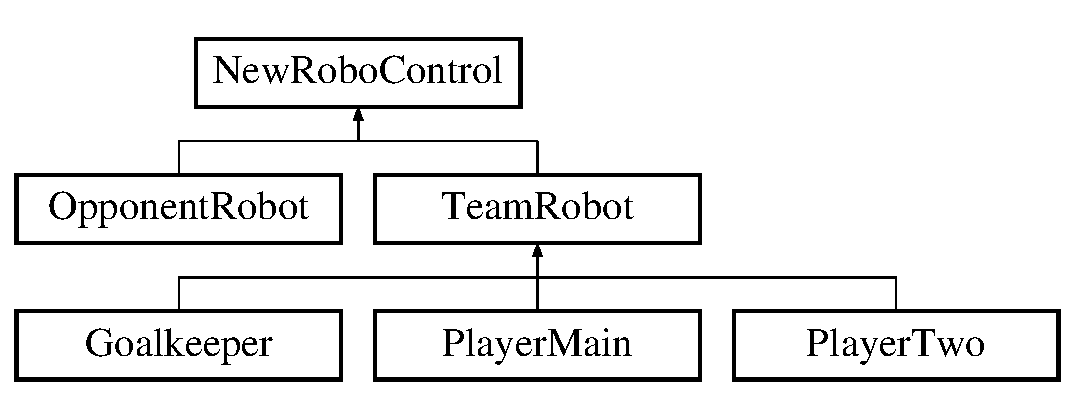
\includegraphics[height=3cm]{classNewRoboControl}
\end{center}
\end{figure}
\subsection*{Public Types}
\begin{DoxyCompactItemize}
\item 
enum \hyperlink{classNewRoboControl_a077fa253b827c190e82c1ce1e4c8d18f}{eDirection} \{ \hyperlink{classNewRoboControl_a077fa253b827c190e82c1ce1e4c8d18fac7af9b70b7504bd260f486172de934d9}{FORWARD}, 
\hyperlink{classNewRoboControl_a077fa253b827c190e82c1ce1e4c8d18faa55a679c9e8fbc7400c88ce3cab09c48}{BACKWARD}
 \}
\end{DoxyCompactItemize}
\subsection*{Public Member Functions}
\begin{DoxyCompactItemize}
\item 
\hyperlink{classNewRoboControl_a81f7ad52f88ea8fb90eeff5650efa1c5}{NewRoboControl} (RTDBConn \&DBC, const int deviceNr)
\item 
virtual \hyperlink{classNewRoboControl_ae63cbd6c60d37882d176e9e7d60b11ba}{$\sim$NewRoboControl} ()=0
\item 
bool \hyperlink{classNewRoboControl_a77b0e86bef15f3b1fb6cf98d91c6a9b4}{IsOnTarget} (Position target, bool precise=true) const 
\item 
bool \hyperlink{classNewRoboControl_a89119d6af9d59b6e0279b39e23c35122}{cruisetoBias} (double tarX, double tarY, int speed, double tarP=-\/10, double varDir=30)
\item 
void \hyperlink{classNewRoboControl_ab3231acd7efd60677b4f48b094cb6dd3}{RandomMove} ()
\item 
bool \hyperlink{classNewRoboControl_a9816eae1b7c90dbb74a7e0365e2b57e9}{drivePath} (std::vector$<$ Position $>$ $\ast$path)
\item 
void \hyperlink{classNewRoboControl_ad2ddddb5f0272a733021524ebaaaeffd}{setSpeed} (double translation, double rotation, \hyperlink{classNewRoboControl_a077fa253b827c190e82c1ce1e4c8d18f}{eDirection} dir)
\end{DoxyCompactItemize}
\subsection*{Static Public Member Functions}
\begin{DoxyCompactItemize}
\item 
static \hyperlink{classNewRoboControl_a077fa253b827c190e82c1ce1e4c8d18f}{eDirection} \hyperlink{classNewRoboControl_a9979ccfbc622d9082fb034caf36c514b}{getDirection} (double nominal, double actual)
\item 
static double \hyperlink{classNewRoboControl_a960c714f4f8828d16dc955c871affbb5}{getDiffAngle} (double nominal, double actual)
\item 
static double \hyperlink{classNewRoboControl_ab2f2407b40c535ed734049e8e1ed71e6}{getSpeedP} (double nominal, double actual)
\item 
static double \hyperlink{classNewRoboControl_ac1f5cb8932193d5e8315bb19aeddb3fa}{getSpeedPt} (double nominal, double actual, int geschw)
\item 
static double \hyperlink{classNewRoboControl_a0c5f29bb2dee1faf96725b80ddc64398}{getSpeedT} (double diff)
\item 
static double \hyperlink{classNewRoboControl_a44def2cefef0f6c41b180bda044dfdfb}{degToRad} (double deg)
\item 
static bool \hyperlink{classNewRoboControl_a106c7ccc03f05693a07da1235ab0b17f}{IsOnTarget} (Position current, Position target, bool precise=true)
\end{DoxyCompactItemize}
\subsection*{Private Attributes}
\begin{DoxyCompactItemize}
\item 
bool \hyperlink{classNewRoboControl_a2f7afe3fa8d85f8fedf05ba12ec21f32}{m\_\-stopCruisingNow}
\item 
bool \hyperlink{classNewRoboControl_aa83c55c4b75ef04c909038e2ad581e3b}{m\_\-isCruising}
\item 
pthread\_\-t \hyperlink{classNewRoboControl_a285a033aa3238a589d78243ce7cdb620}{m\_\-cruiseThread}
\end{DoxyCompactItemize}


\subsection{Member Enumeration Documentation}
\hypertarget{classNewRoboControl_a077fa253b827c190e82c1ce1e4c8d18f}{
\index{NewRoboControl@{NewRoboControl}!eDirection@{eDirection}}
\index{eDirection@{eDirection}!NewRoboControl@{NewRoboControl}}
\subsubsection[{eDirection}]{\setlength{\rightskip}{0pt plus 5cm}enum {\bf NewRoboControl::eDirection}}}
\label{classNewRoboControl_a077fa253b827c190e82c1ce1e4c8d18f}
\begin{Desc}
\item[Enumerator: ]\par
\begin{description}
\index{FORWARD@{FORWARD}!NewRoboControl@{NewRoboControl}}\index{NewRoboControl@{NewRoboControl}!FORWARD@{FORWARD}}\item[{\em 
\hypertarget{classNewRoboControl_a077fa253b827c190e82c1ce1e4c8d18fac7af9b70b7504bd260f486172de934d9}{
FORWARD}
\label{classNewRoboControl_a077fa253b827c190e82c1ce1e4c8d18fac7af9b70b7504bd260f486172de934d9}
}]TODO \index{BACKWARD@{BACKWARD}!NewRoboControl@{NewRoboControl}}\index{NewRoboControl@{NewRoboControl}!BACKWARD@{BACKWARD}}\item[{\em 
\hypertarget{classNewRoboControl_a077fa253b827c190e82c1ce1e4c8d18faa55a679c9e8fbc7400c88ce3cab09c48}{
BACKWARD}
\label{classNewRoboControl_a077fa253b827c190e82c1ce1e4c8d18faa55a679c9e8fbc7400c88ce3cab09c48}
}]TODO \end{description}
\end{Desc}



\subsection{Constructor \& Destructor Documentation}
\hypertarget{classNewRoboControl_a81f7ad52f88ea8fb90eeff5650efa1c5}{
\index{NewRoboControl@{NewRoboControl}!NewRoboControl@{NewRoboControl}}
\index{NewRoboControl@{NewRoboControl}!NewRoboControl@{NewRoboControl}}
\subsubsection[{NewRoboControl}]{\setlength{\rightskip}{0pt plus 5cm}NewRoboControl::NewRoboControl (RTDBConn \& {\em DBC}, \/  const int {\em deviceNr})}}
\label{classNewRoboControl_a81f7ad52f88ea8fb90eeff5650efa1c5}

\begin{DoxyParams}{Parameters}
\item[{\em DBC}]\item[{\em deviceNr}]\end{DoxyParams}
\hypertarget{classNewRoboControl_ae63cbd6c60d37882d176e9e7d60b11ba}{
\index{NewRoboControl@{NewRoboControl}!$\sim$NewRoboControl@{$\sim$NewRoboControl}}
\index{$\sim$NewRoboControl@{$\sim$NewRoboControl}!NewRoboControl@{NewRoboControl}}
\subsubsection[{$\sim$NewRoboControl}]{\setlength{\rightskip}{0pt plus 5cm}NewRoboControl::$\sim$NewRoboControl ()\hspace{0.3cm}{\ttfamily  \mbox{[}pure virtual\mbox{]}}}}
\label{classNewRoboControl_ae63cbd6c60d37882d176e9e7d60b11ba}


\subsection{Member Function Documentation}
\hypertarget{classNewRoboControl_a89119d6af9d59b6e0279b39e23c35122}{
\index{NewRoboControl@{NewRoboControl}!cruisetoBias@{cruisetoBias}}
\index{cruisetoBias@{cruisetoBias}!NewRoboControl@{NewRoboControl}}
\subsubsection[{cruisetoBias}]{\setlength{\rightskip}{0pt plus 5cm}bool NewRoboControl::cruisetoBias (double {\em tarX}, \/  double {\em tarY}, \/  int {\em speed}, \/  double {\em tarP} = {\ttfamily -\/10}, \/  double {\em varDir} = {\ttfamily 30})}}
\label{classNewRoboControl_a89119d6af9d59b6e0279b39e23c35122}

\begin{DoxyParams}{Parameters}
\item[{\em tarX}]\item[{\em tarY}]\item[{\em speed}]\item[{\em tarP}]\item[{\em varDir}]\end{DoxyParams}
\begin{DoxyReturn}{Returns}
bool 
\end{DoxyReturn}
\hypertarget{classNewRoboControl_a44def2cefef0f6c41b180bda044dfdfb}{
\index{NewRoboControl@{NewRoboControl}!degToRad@{degToRad}}
\index{degToRad@{degToRad}!NewRoboControl@{NewRoboControl}}
\subsubsection[{degToRad}]{\setlength{\rightskip}{0pt plus 5cm}double NewRoboControl::degToRad (double {\em deg})\hspace{0.3cm}{\ttfamily  \mbox{[}static\mbox{]}}}}
\label{classNewRoboControl_a44def2cefef0f6c41b180bda044dfdfb}

\begin{DoxyParams}{Parameters}
\item[{\em deg}]\end{DoxyParams}
\begin{DoxyReturn}{Returns}
double 
\end{DoxyReturn}
\hypertarget{classNewRoboControl_a9816eae1b7c90dbb74a7e0365e2b57e9}{
\index{NewRoboControl@{NewRoboControl}!drivePath@{drivePath}}
\index{drivePath@{drivePath}!NewRoboControl@{NewRoboControl}}
\subsubsection[{drivePath}]{\setlength{\rightskip}{0pt plus 5cm}bool NewRoboControl::drivePath (std::vector$<$ Position $>$ $\ast$ {\em path})}}
\label{classNewRoboControl_a9816eae1b7c90dbb74a7e0365e2b57e9}

\begin{DoxyParams}{Parameters}
\item[{\em path}]\end{DoxyParams}
\begin{DoxyReturn}{Returns}
bool 
\end{DoxyReturn}
\hypertarget{classNewRoboControl_a960c714f4f8828d16dc955c871affbb5}{
\index{NewRoboControl@{NewRoboControl}!getDiffAngle@{getDiffAngle}}
\index{getDiffAngle@{getDiffAngle}!NewRoboControl@{NewRoboControl}}
\subsubsection[{getDiffAngle}]{\setlength{\rightskip}{0pt plus 5cm}double NewRoboControl::getDiffAngle (double {\em nominal}, \/  double {\em actual})\hspace{0.3cm}{\ttfamily  \mbox{[}static\mbox{]}}}}
\label{classNewRoboControl_a960c714f4f8828d16dc955c871affbb5}

\begin{DoxyParams}{Parameters}
\item[{\em nominal}]\item[{\em actual}]\end{DoxyParams}
\begin{DoxyReturn}{Returns}
double 
\end{DoxyReturn}
\hypertarget{classNewRoboControl_a9979ccfbc622d9082fb034caf36c514b}{
\index{NewRoboControl@{NewRoboControl}!getDirection@{getDirection}}
\index{getDirection@{getDirection}!NewRoboControl@{NewRoboControl}}
\subsubsection[{getDirection}]{\setlength{\rightskip}{0pt plus 5cm}{\bf NewRoboControl::eDirection} NewRoboControl::getDirection (double {\em nominal}, \/  double {\em actual})\hspace{0.3cm}{\ttfamily  \mbox{[}static\mbox{]}}}}
\label{classNewRoboControl_a9979ccfbc622d9082fb034caf36c514b}

\begin{DoxyParams}{Parameters}
\item[{\em nominal}]\item[{\em actual}]\end{DoxyParams}
\begin{DoxyReturn}{Returns}
Controller::eDirection 
\end{DoxyReturn}
\hypertarget{classNewRoboControl_ab2f2407b40c535ed734049e8e1ed71e6}{
\index{NewRoboControl@{NewRoboControl}!getSpeedP@{getSpeedP}}
\index{getSpeedP@{getSpeedP}!NewRoboControl@{NewRoboControl}}
\subsubsection[{getSpeedP}]{\setlength{\rightskip}{0pt plus 5cm}double NewRoboControl::getSpeedP (double {\em nominal}, \/  double {\em actual})\hspace{0.3cm}{\ttfamily  \mbox{[}static\mbox{]}}}}
\label{classNewRoboControl_ab2f2407b40c535ed734049e8e1ed71e6}

\begin{DoxyParams}{Parameters}
\item[{\em nominal}]\item[{\em actual}]\end{DoxyParams}
\begin{DoxyReturn}{Returns}
double 
\end{DoxyReturn}
\hypertarget{classNewRoboControl_ac1f5cb8932193d5e8315bb19aeddb3fa}{
\index{NewRoboControl@{NewRoboControl}!getSpeedPt@{getSpeedPt}}
\index{getSpeedPt@{getSpeedPt}!NewRoboControl@{NewRoboControl}}
\subsubsection[{getSpeedPt}]{\setlength{\rightskip}{0pt plus 5cm}double NewRoboControl::getSpeedPt (double {\em nominal}, \/  double {\em actual}, \/  int {\em geschw})\hspace{0.3cm}{\ttfamily  \mbox{[}static\mbox{]}}}}
\label{classNewRoboControl_ac1f5cb8932193d5e8315bb19aeddb3fa}

\begin{DoxyParams}{Parameters}
\item[{\em nominal}]\item[{\em actual}]\end{DoxyParams}
\begin{DoxyReturn}{Returns}
double 
\end{DoxyReturn}
\hypertarget{classNewRoboControl_a0c5f29bb2dee1faf96725b80ddc64398}{
\index{NewRoboControl@{NewRoboControl}!getSpeedT@{getSpeedT}}
\index{getSpeedT@{getSpeedT}!NewRoboControl@{NewRoboControl}}
\subsubsection[{getSpeedT}]{\setlength{\rightskip}{0pt plus 5cm}double NewRoboControl::getSpeedT (double {\em diff})\hspace{0.3cm}{\ttfamily  \mbox{[}static\mbox{]}}}}
\label{classNewRoboControl_a0c5f29bb2dee1faf96725b80ddc64398}

\begin{DoxyParams}{Parameters}
\item[{\em diff}]\end{DoxyParams}
\begin{DoxyReturn}{Returns}
double 
\end{DoxyReturn}
\hypertarget{classNewRoboControl_a77b0e86bef15f3b1fb6cf98d91c6a9b4}{
\index{NewRoboControl@{NewRoboControl}!IsOnTarget@{IsOnTarget}}
\index{IsOnTarget@{IsOnTarget}!NewRoboControl@{NewRoboControl}}
\subsubsection[{IsOnTarget}]{\setlength{\rightskip}{0pt plus 5cm}bool NewRoboControl::IsOnTarget (Position {\em target}, \/  bool {\em precise} = {\ttfamily true}) const}}
\label{classNewRoboControl_a77b0e86bef15f3b1fb6cf98d91c6a9b4}

\begin{DoxyParams}{Parameters}
\item[{\em target}]\item[{\em precise}]\end{DoxyParams}
\begin{DoxyReturn}{Returns}
bool 
\end{DoxyReturn}
\hypertarget{classNewRoboControl_a106c7ccc03f05693a07da1235ab0b17f}{
\index{NewRoboControl@{NewRoboControl}!IsOnTarget@{IsOnTarget}}
\index{IsOnTarget@{IsOnTarget}!NewRoboControl@{NewRoboControl}}
\subsubsection[{IsOnTarget}]{\setlength{\rightskip}{0pt plus 5cm}bool NewRoboControl::IsOnTarget (Position {\em current}, \/  Position {\em target}, \/  bool {\em precise} = {\ttfamily true})\hspace{0.3cm}{\ttfamily  \mbox{[}static\mbox{]}}}}
\label{classNewRoboControl_a106c7ccc03f05693a07da1235ab0b17f}

\begin{DoxyParams}{Parameters}
\item[{\em current}]\item[{\em target}]\item[{\em precise}]\end{DoxyParams}
\begin{DoxyReturn}{Returns}
bool 
\end{DoxyReturn}
\hypertarget{classNewRoboControl_ab3231acd7efd60677b4f48b094cb6dd3}{
\index{NewRoboControl@{NewRoboControl}!RandomMove@{RandomMove}}
\index{RandomMove@{RandomMove}!NewRoboControl@{NewRoboControl}}
\subsubsection[{RandomMove}]{\setlength{\rightskip}{0pt plus 5cm}void NewRoboControl::RandomMove ()}}
\label{classNewRoboControl_ab3231acd7efd60677b4f48b094cb6dd3}
\hypertarget{classNewRoboControl_ad2ddddb5f0272a733021524ebaaaeffd}{
\index{NewRoboControl@{NewRoboControl}!setSpeed@{setSpeed}}
\index{setSpeed@{setSpeed}!NewRoboControl@{NewRoboControl}}
\subsubsection[{setSpeed}]{\setlength{\rightskip}{0pt plus 5cm}void NewRoboControl::setSpeed (double {\em translation}, \/  double {\em rotation}, \/  {\bf eDirection} {\em dir})}}
\label{classNewRoboControl_ad2ddddb5f0272a733021524ebaaaeffd}

\begin{DoxyParams}{Parameters}
\item[{\em translation}]\item[{\em rotation}]\item[{\em dir}]\end{DoxyParams}


\subsection{Member Data Documentation}
\hypertarget{classNewRoboControl_a285a033aa3238a589d78243ce7cdb620}{
\index{NewRoboControl@{NewRoboControl}!m\_\-cruiseThread@{m\_\-cruiseThread}}
\index{m\_\-cruiseThread@{m\_\-cruiseThread}!NewRoboControl@{NewRoboControl}}
\subsubsection[{m\_\-cruiseThread}]{\setlength{\rightskip}{0pt plus 5cm}pthread\_\-t {\bf NewRoboControl::m\_\-cruiseThread}\hspace{0.3cm}{\ttfamily  \mbox{[}private\mbox{]}}}}
\label{classNewRoboControl_a285a033aa3238a589d78243ce7cdb620}
TODO \hypertarget{classNewRoboControl_aa83c55c4b75ef04c909038e2ad581e3b}{
\index{NewRoboControl@{NewRoboControl}!m\_\-isCruising@{m\_\-isCruising}}
\index{m\_\-isCruising@{m\_\-isCruising}!NewRoboControl@{NewRoboControl}}
\subsubsection[{m\_\-isCruising}]{\setlength{\rightskip}{0pt plus 5cm}bool {\bf NewRoboControl::m\_\-isCruising}\hspace{0.3cm}{\ttfamily  \mbox{[}private\mbox{]}}}}
\label{classNewRoboControl_aa83c55c4b75ef04c909038e2ad581e3b}
TODO \hypertarget{classNewRoboControl_a2f7afe3fa8d85f8fedf05ba12ec21f32}{
\index{NewRoboControl@{NewRoboControl}!m\_\-stopCruisingNow@{m\_\-stopCruisingNow}}
\index{m\_\-stopCruisingNow@{m\_\-stopCruisingNow}!NewRoboControl@{NewRoboControl}}
\subsubsection[{m\_\-stopCruisingNow}]{\setlength{\rightskip}{0pt plus 5cm}bool {\bf NewRoboControl::m\_\-stopCruisingNow}\hspace{0.3cm}{\ttfamily  \mbox{[}private\mbox{]}}}}
\label{classNewRoboControl_a2f7afe3fa8d85f8fedf05ba12ec21f32}
TODO 

The documentation for this class was generated from the following files:\begin{DoxyCompactItemize}
\item 
src/\hyperlink{newrobocontrol_8h}{newrobocontrol.h}\item 
src/\hyperlink{newrobocontrol_8cpp}{newrobocontrol.cpp}\end{DoxyCompactItemize}

\hypertarget{classnode}{
\section{node Class Reference}
\label{classnode}\index{node@{node}}
}


{\ttfamily \#include $<$node.h$>$}

\subsection*{Public Member Functions}
\begin{DoxyCompactItemize}
\item 
\hyperlink{classnode_a802701cab6639590de6f16136184c2de}{node} (int xp, int yp, int d, int p)
\item 
int \hyperlink{classnode_a419596f9858640ee6d04b69b616b7cd2}{getxPos} () const 
\item 
int \hyperlink{classnode_a3b5d135d5e5eac9211a9478ea9803ae7}{getyPos} () const 
\item 
int \hyperlink{classnode_a78c66d7badca074b6b34ec7eca4ab106}{getLevel} () const 
\item 
int \hyperlink{classnode_afebf5ef7f94fa7554890f03e97686de7}{getPriority} () const 
\item 
void \hyperlink{classnode_ad51b92de008bd5107a7b55cc61fc497b}{updatePriority} (const int \&xDest, const int \&yDest)
\item 
void \hyperlink{classnode_a04a186013c42fb942b6da90d2e98d4ed}{nextLevel} (const int \&i)
\item 
const int \& \hyperlink{classnode_a311569dff2e77c4c7953107333960a5d}{estimate} (const int \&xDest, const int \&yDest) const 
\end{DoxyCompactItemize}
\subsection*{Private Attributes}
\begin{DoxyCompactItemize}
\item 
int \hyperlink{classnode_a377c0cd9462931487ee9a80917c0071a}{m\_\-xPos}
\item 
int \hyperlink{classnode_a848f211f150104a88c1e072c4716f169}{m\_\-yPos}
\item 
int \hyperlink{classnode_ab68076929ea68209db1fdd25b7530515}{m\_\-level}
\item 
int \hyperlink{classnode_ae1c537b9584f180d868a0ddf1b64526c}{m\_\-priority}
\end{DoxyCompactItemize}


\subsection{Constructor \& Destructor Documentation}
\hypertarget{classnode_a802701cab6639590de6f16136184c2de}{
\index{node@{node}!node@{node}}
\index{node@{node}!node@{node}}
\subsubsection[{node}]{\setlength{\rightskip}{0pt plus 5cm}node::node (int {\em xp}, \/  int {\em yp}, \/  int {\em d}, \/  int {\em p})}}
\label{classnode_a802701cab6639590de6f16136184c2de}

\begin{DoxyParams}{Parameters}
\item[{\em xp}]\item[{\em yp}]\item[{\em d}]\item[{\em p}]\end{DoxyParams}


\subsection{Member Function Documentation}
\hypertarget{classnode_a311569dff2e77c4c7953107333960a5d}{
\index{node@{node}!estimate@{estimate}}
\index{estimate@{estimate}!node@{node}}
\subsubsection[{estimate}]{\setlength{\rightskip}{0pt plus 5cm}const int \& node::estimate (const int \& {\em xDest}, \/  const int \& {\em yDest}) const}}
\label{classnode_a311569dff2e77c4c7953107333960a5d}

\begin{DoxyParams}{Parameters}
\item[{\em xDest}]\item[{\em yDest}]\end{DoxyParams}
\begin{DoxyReturn}{Returns}
const int \& 
\end{DoxyReturn}
\hypertarget{classnode_a78c66d7badca074b6b34ec7eca4ab106}{
\index{node@{node}!getLevel@{getLevel}}
\index{getLevel@{getLevel}!node@{node}}
\subsubsection[{getLevel}]{\setlength{\rightskip}{0pt plus 5cm}int node::getLevel () const}}
\label{classnode_a78c66d7badca074b6b34ec7eca4ab106}
\begin{DoxyReturn}{Returns}
int 
\end{DoxyReturn}
\hypertarget{classnode_afebf5ef7f94fa7554890f03e97686de7}{
\index{node@{node}!getPriority@{getPriority}}
\index{getPriority@{getPriority}!node@{node}}
\subsubsection[{getPriority}]{\setlength{\rightskip}{0pt plus 5cm}int node::getPriority () const}}
\label{classnode_afebf5ef7f94fa7554890f03e97686de7}
\begin{DoxyReturn}{Returns}
int 
\end{DoxyReturn}
\hypertarget{classnode_a419596f9858640ee6d04b69b616b7cd2}{
\index{node@{node}!getxPos@{getxPos}}
\index{getxPos@{getxPos}!node@{node}}
\subsubsection[{getxPos}]{\setlength{\rightskip}{0pt plus 5cm}int node::getxPos () const}}
\label{classnode_a419596f9858640ee6d04b69b616b7cd2}
\begin{DoxyReturn}{Returns}
int 
\end{DoxyReturn}
\hypertarget{classnode_a3b5d135d5e5eac9211a9478ea9803ae7}{
\index{node@{node}!getyPos@{getyPos}}
\index{getyPos@{getyPos}!node@{node}}
\subsubsection[{getyPos}]{\setlength{\rightskip}{0pt plus 5cm}int node::getyPos () const}}
\label{classnode_a3b5d135d5e5eac9211a9478ea9803ae7}
\begin{DoxyReturn}{Returns}
int 
\end{DoxyReturn}
\hypertarget{classnode_a04a186013c42fb942b6da90d2e98d4ed}{
\index{node@{node}!nextLevel@{nextLevel}}
\index{nextLevel@{nextLevel}!node@{node}}
\subsubsection[{nextLevel}]{\setlength{\rightskip}{0pt plus 5cm}void node::nextLevel (const int \& {\em i})}}
\label{classnode_a04a186013c42fb942b6da90d2e98d4ed}

\begin{DoxyParams}{Parameters}
\item[{\em i}]\end{DoxyParams}
\hypertarget{classnode_ad51b92de008bd5107a7b55cc61fc497b}{
\index{node@{node}!updatePriority@{updatePriority}}
\index{updatePriority@{updatePriority}!node@{node}}
\subsubsection[{updatePriority}]{\setlength{\rightskip}{0pt plus 5cm}void node::updatePriority (const int \& {\em xDest}, \/  const int \& {\em yDest})}}
\label{classnode_ad51b92de008bd5107a7b55cc61fc497b}

\begin{DoxyParams}{Parameters}
\item[{\em xDest}]\item[{\em yDest}]\end{DoxyParams}


\subsection{Member Data Documentation}
\hypertarget{classnode_ab68076929ea68209db1fdd25b7530515}{
\index{node@{node}!m\_\-level@{m\_\-level}}
\index{m\_\-level@{m\_\-level}!node@{node}}
\subsubsection[{m\_\-level}]{\setlength{\rightskip}{0pt plus 5cm}int {\bf node::m\_\-level}\hspace{0.3cm}{\ttfamily  \mbox{[}private\mbox{]}}}}
\label{classnode_ab68076929ea68209db1fdd25b7530515}
Total distance already travelled to reach the node \hypertarget{classnode_ae1c537b9584f180d868a0ddf1b64526c}{
\index{node@{node}!m\_\-priority@{m\_\-priority}}
\index{m\_\-priority@{m\_\-priority}!node@{node}}
\subsubsection[{m\_\-priority}]{\setlength{\rightskip}{0pt plus 5cm}int {\bf node::m\_\-priority}\hspace{0.3cm}{\ttfamily  \mbox{[}private\mbox{]}}}}
\label{classnode_ae1c537b9584f180d868a0ddf1b64526c}
Level + remaining distance estimate (smaller: higher priority) \hypertarget{classnode_a377c0cd9462931487ee9a80917c0071a}{
\index{node@{node}!m\_\-xPos@{m\_\-xPos}}
\index{m\_\-xPos@{m\_\-xPos}!node@{node}}
\subsubsection[{m\_\-xPos}]{\setlength{\rightskip}{0pt plus 5cm}int {\bf node::m\_\-xPos}\hspace{0.3cm}{\ttfamily  \mbox{[}private\mbox{]}}}}
\label{classnode_a377c0cd9462931487ee9a80917c0071a}
Current position (x coordinate) \hypertarget{classnode_a848f211f150104a88c1e072c4716f169}{
\index{node@{node}!m\_\-yPos@{m\_\-yPos}}
\index{m\_\-yPos@{m\_\-yPos}!node@{node}}
\subsubsection[{m\_\-yPos}]{\setlength{\rightskip}{0pt plus 5cm}int {\bf node::m\_\-yPos}\hspace{0.3cm}{\ttfamily  \mbox{[}private\mbox{]}}}}
\label{classnode_a848f211f150104a88c1e072c4716f169}
Current position (y coordinate) 

The documentation for this class was generated from the following files:\begin{DoxyCompactItemize}
\item 
src/\hyperlink{node_8h}{node.h}\item 
src/\hyperlink{node_8cpp}{node.cpp}\end{DoxyCompactItemize}

\hypertarget{classOpponentRobot}{
\section{OpponentRobot Class Reference}
\label{classOpponentRobot}\index{OpponentRobot@{OpponentRobot}}
}


Child class of \hyperlink{classNewRoboControl}{NewRoboControl} which desribes a robo of the other team.  




{\ttfamily \#include $<$opponentrobot.h$>$}



Inheritance diagram for OpponentRobot:\nopagebreak
\begin{figure}[H]
\begin{center}
\leavevmode
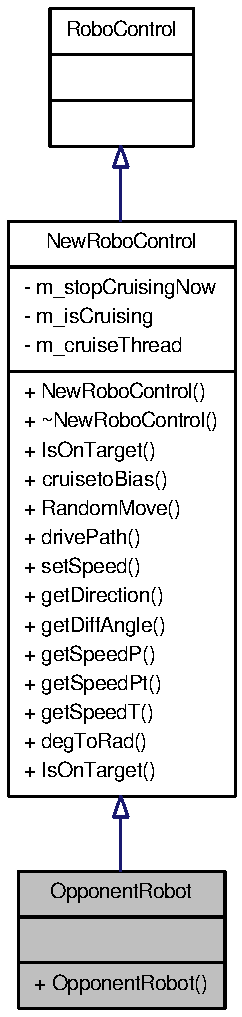
\includegraphics[height=400pt]{classOpponentRobot__inherit__graph}
\end{center}
\end{figure}
\subsection*{Public Member Functions}
\begin{DoxyCompactItemize}
\item 
\hyperlink{classOpponentRobot_a315c08a9f17d278b1bb8067929b38f83}{OpponentRobot} (RTDBConn \&DBC, const int deviceNr)
\begin{DoxyCompactList}\small\item\em Basic constructor. \item\end{DoxyCompactList}\end{DoxyCompactItemize}


\subsection{Detailed Description}
Child class of \hyperlink{classNewRoboControl}{NewRoboControl} which desribes a robo of the other team. This class does not implement anything and is just used to make the distinction with a \hyperlink{classTeamRobot}{TeamRobot}. It is however still possible to use the driving functions of the parents \hyperlink{classNewRoboControl}{NewRoboControl} and \char`\"{}RoboControl\char`\"{}, but this should be avoided as it is forbidden by the game rules. 

\subsection{Constructor \& Destructor Documentation}
\hypertarget{classOpponentRobot_a315c08a9f17d278b1bb8067929b38f83}{
\index{OpponentRobot@{OpponentRobot}!OpponentRobot@{OpponentRobot}}
\index{OpponentRobot@{OpponentRobot}!OpponentRobot@{OpponentRobot}}
\subsubsection[{OpponentRobot}]{\setlength{\rightskip}{0pt plus 5cm}OpponentRobot::OpponentRobot (RTDBConn \& {\em DBC}, \/  const int {\em deviceNr})}}
\label{classOpponentRobot_a315c08a9f17d278b1bb8067929b38f83}


Basic constructor. 


\begin{DoxyParams}{Parameters}
\item[{\em DBC}]\item[{\em deviceNr}]\end{DoxyParams}


The documentation for this class was generated from the following files:\begin{DoxyCompactItemize}
\item 
src/\hyperlink{opponentrobot_8h}{opponentrobot.h}\item 
src/\hyperlink{opponentrobot_8cpp}{opponentrobot.cpp}\end{DoxyCompactItemize}

\hypertarget{classPathFinder}{
\section{PathFinder Class Reference}
\label{classPathFinder}\index{PathFinder@{PathFinder}}
}


Class used to find the shortest path in a given environment.  




{\ttfamily \#include $<$pathfinder.h$>$}

\subsection*{Classes}
\begin{DoxyCompactItemize}
\item 
struct \hyperlink{structPathFinder_1_1ConvexPolygon}{ConvexPolygon}
\begin{DoxyCompactList}\small\item\em Structure used to represent a convex polygon. \item\end{DoxyCompactList}\item 
struct \hyperlink{structPathFinder_1_1Point}{Point}
\begin{DoxyCompactList}\small\item\em Structure to represent a point in the path finder. \item\end{DoxyCompactList}\item 
struct \hyperlink{structPathFinder_1_1Rectangle}{Rectangle}
\begin{DoxyCompactList}\small\item\em Structure used to represent a horizontal rectangle. \item\end{DoxyCompactList}\item 
struct \hyperlink{structPathFinder_1_1Segment}{Segment}
\begin{DoxyCompactList}\small\item\em Structure used to describe a line segment. \item\end{DoxyCompactList}\end{DoxyCompactItemize}
\subsection*{Public Types}
\begin{DoxyCompactItemize}
\item 
typedef std::vector$<$ \hyperlink{structPathFinder_1_1ConvexPolygon}{ConvexPolygon} $\ast$ $>$ \hyperlink{classPathFinder_a16ed073fa542c82fd09e582cb4fbed24}{PolygonsList}
\begin{DoxyCompactList}\small\item\em Type to store a list of \hyperlink{structPathFinder_1_1ConvexPolygon}{convex polygons}. Stores pointers to the polygons. \item\end{DoxyCompactList}\item 
typedef std::vector$<$ \hyperlink{structPathFinder_1_1Point}{Point} $\ast$ $>$ \hyperlink{classPathFinder_a792a34ce673309f873090141c3d96f1c}{PointsList}
\begin{DoxyCompactList}\small\item\em Type to store a list of \hyperlink{structPathFinder_1_1Point}{points}. Stores pointers to the points. \item\end{DoxyCompactList}\item 
typedef std::vector$<$ \hyperlink{structPathFinder_1_1Point}{Point} $>$ $\ast$ \hyperlink{classPathFinder_a269aba09b7b3208092f67f2bc02cf63e}{Path}
\begin{DoxyCompactList}\small\item\em Type used to represent a full path. Pointer to a list of \hyperlink{structPathFinder_1_1Point}{points}. \item\end{DoxyCompactList}\end{DoxyCompactItemize}
\subsection*{Public Member Functions}
\begin{DoxyCompactItemize}
\item 
\hyperlink{classPathFinder_a0761f248c1ebaacf3e47a4021ca25256}{PathFinder} ()
\begin{DoxyCompactList}\small\item\em Default (and unique) constructor for the path finder. \item\end{DoxyCompactList}\item 
\hyperlink{classPathFinder_acc04bc8bcddfda54da6a2905b256cf90}{$\sim$PathFinder} ()
\begin{DoxyCompactList}\small\item\em Destructor of the path finder. \item\end{DoxyCompactList}\item 
const \hyperlink{structPathFinder_1_1ConvexPolygon}{ConvexPolygon} $\ast$ \hyperlink{classPathFinder_a7b703516042173b63c24759b600d655e}{AddRectangle} (const \hyperlink{structPathFinder_1_1Point}{Point} \&ul, const \hyperlink{structPathFinder_1_1Point}{Point} \&lr)
\begin{DoxyCompactList}\small\item\em Adds a horizontal rectangle to the path finder's world. \item\end{DoxyCompactList}\item 
const \hyperlink{structPathFinder_1_1ConvexPolygon}{ConvexPolygon} $\ast$ \hyperlink{classPathFinder_a85d6d0654ad55f798c4ecc826f7f63de}{AddParallelogram} (const \hyperlink{structPathFinder_1_1Point}{Point} \&ul0, const \hyperlink{structPathFinder_1_1Point}{Point} \&ur0, const \hyperlink{structPathFinder_1_1Point}{Point} \&ll0)
\begin{DoxyCompactList}\small\item\em Adds a parallelogram to the path finder's world. \item\end{DoxyCompactList}\item 
const \hyperlink{structPathFinder_1_1ConvexPolygon}{ConvexPolygon} $\ast$ \hyperlink{classPathFinder_a78778ee12c740256f30907e660c563b3}{AddThickLine} (const \hyperlink{structPathFinder_1_1Point}{Point} \&pt1, const \hyperlink{structPathFinder_1_1Point}{Point} \&pt2, double thickness)
\begin{DoxyCompactList}\small\item\em Adds a \char`\"{}thick line\char`\"{} (rotated rectangle) to the path finder's world. \item\end{DoxyCompactList}\item 
const \hyperlink{structPathFinder_1_1ConvexPolygon}{ConvexPolygon} $\ast$ \hyperlink{classPathFinder_ae167f12c8466a501a5a54068f92328c7}{AddPolygon} (const \hyperlink{structPathFinder_1_1ConvexPolygon}{ConvexPolygon} \&p)
\begin{DoxyCompactList}\small\item\em Adds a \hyperlink{structPathFinder_1_1ConvexPolygon}{convex polygon} to the path finder's world. \item\end{DoxyCompactList}\item 
bool \hyperlink{classPathFinder_adbc8795e40ef601769a2659c241b4cb9}{RemovePolygon} (const \hyperlink{structPathFinder_1_1ConvexPolygon}{ConvexPolygon} $\ast$poly)
\begin{DoxyCompactList}\small\item\em Removes and fully frees a given \hyperlink{structPathFinder_1_1ConvexPolygon}{polygon} from the path finder's world. \item\end{DoxyCompactList}\item 
bool \hyperlink{classPathFinder_a4707e0176f1a42c14f71fabc1cca4927}{RemovePolygons} (const \hyperlink{structPathFinder_1_1ConvexPolygon}{ConvexPolygon} $\ast$polys\mbox{[}$\,$\mbox{]}, int n)
\begin{DoxyCompactList}\small\item\em Removes and fully frees a list of \hyperlink{structPathFinder_1_1ConvexPolygon}{polygons} from the path finder's world. \item\end{DoxyCompactList}\item 
bool \hyperlink{classPathFinder_ae4c46e0856f22121c4ac7bb07cc86dc1}{IsPolygonRegistered} (const \hyperlink{structPathFinder_1_1ConvexPolygon}{ConvexPolygon} $\ast$poly) const 
\begin{DoxyCompactList}\small\item\em Tells if a given \hyperlink{structPathFinder_1_1ConvexPolygon}{polygon} is currenlty in the path finder's world. \item\end{DoxyCompactList}\item 
bool \hyperlink{classPathFinder_a6f0e23839f34803a1e712ff727ec734f}{IsPointRegistered} (const \hyperlink{structPathFinder_1_1Point}{Point} $\ast$pt) const 
\begin{DoxyCompactList}\small\item\em Tells if a given \hyperlink{structPathFinder_1_1Point}{point} is currently in the path finder's world. \item\end{DoxyCompactList}\item 
const std::vector$<$ \hyperlink{structPathFinder_1_1ConvexPolygon}{ConvexPolygon} $\ast$ $>$ \& \hyperlink{classPathFinder_a61256a9d84ff19f3471f0b22f69527e2}{GetPolygons} () const 
\begin{DoxyCompactList}\small\item\em Returns a list of every \hyperlink{structPathFinder_1_1ConvexPolygon}{polygon} currently in the path finder's world. \item\end{DoxyCompactList}\item 
\hyperlink{classPathFinder_a16ed073fa542c82fd09e582cb4fbed24}{PolygonsList} \hyperlink{classPathFinder_a1341f2c71d9984cc73719c8d9aa6aaa2}{GetPolygonsCopy} () const 
\begin{DoxyCompactList}\small\item\em Returns a list of every \hyperlink{structPathFinder_1_1ConvexPolygon}{polygon} currently in the path finder's world. \item\end{DoxyCompactList}\item 
std::vector$<$ \hyperlink{structPathFinder_1_1Point}{Point} $>$ $\ast$ \hyperlink{classPathFinder_a7d1904c4ee6abc79375356dc64cad995}{ComputePath} (\hyperlink{structPathFinder_1_1Point}{Point} start, \hyperlink{structPathFinder_1_1Point}{Point} end)
\begin{DoxyCompactList}\small\item\em Computes the shortest path between two given \hyperlink{structPathFinder_1_1Point}{points} in the path finder's world. \item\end{DoxyCompactList}\item 
bool \hyperlink{classPathFinder_a6d04d3b16677670873ea607c7966f49f}{CheckPointsVisibility} (const \hyperlink{structPathFinder_1_1Point}{Point} $\ast$p1, const \hyperlink{structPathFinder_1_1Point}{Point} $\ast$p2)
\begin{DoxyCompactList}\small\item\em Thread-\/safe wrapper for \hyperlink{classPathFinder_a12fb7b7f54766d8bbf5753a5a036a5f0}{PathFinder::CheckPointsVisibility\_\-p()}. \item\end{DoxyCompactList}\item 
\hyperlink{structPathFinder_1_1Point}{Point} \hyperlink{classPathFinder_a1ea7cda7d83a2474efa4af71f0025d94}{ComputeClosestAccessiblePoint} (const \hyperlink{structPathFinder_1_1Point}{Point} \&start, const \hyperlink{structPathFinder_1_1Point}{Point} \&end)
\begin{DoxyCompactList}\small\item\em Computes the closest \hyperlink{structPathFinder_1_1Point}{point} to a given point, which is accessible from another point. \item\end{DoxyCompactList}\end{DoxyCompactItemize}
\subsection*{Static Public Member Functions}
\begin{DoxyCompactItemize}
\item 
static \hyperlink{structPathFinder_1_1Point}{Point} \hyperlink{classPathFinder_a457592f3579bbe0c0527360c2c8a928a}{CreatePoint} (double x, double y)
\begin{DoxyCompactList}\small\item\em Creates a \hyperlink{structPathFinder_1_1Point}{point}. This function should always be used to create points. \item\end{DoxyCompactList}\item 
static \hyperlink{classPathFinder_a269aba09b7b3208092f67f2bc02cf63e}{Path} \hyperlink{classPathFinder_a42e557e3fe4cd1b209a4722ecfbf876b}{CreatePath} (\hyperlink{structPathFinder_1_1Point}{Point} start, \hyperlink{structPathFinder_1_1Point}{Point} end)
\begin{DoxyCompactList}\small\item\em Creates a \hyperlink{classPathFinder_a269aba09b7b3208092f67f2bc02cf63e}{path} with the two given \hyperlink{structPathFinder_1_1Point}{points}. \item\end{DoxyCompactList}\item 
static std::vector$<$ Position $>$ $\ast$ \hyperlink{classPathFinder_aba7f833c9bb8de011c62a1f01fb26144}{ConvertPathToReal} (const \hyperlink{classPathFinder_a269aba09b7b3208092f67f2bc02cf63e}{Path} path, const \hyperlink{classCoordinatesCalibrer}{CoordinatesCalibrer} $\ast$calibrer=NULL)
\begin{DoxyCompactList}\small\item\em Converts a \hyperlink{classPathFinder_a269aba09b7b3208092f67f2bc02cf63e}{path} to a list of positions. \item\end{DoxyCompactList}\item 
static void \hyperlink{classPathFinder_a3306e3d1bb0ae88e236eb7cabbfce835}{DestroyPolygonsList} (\hyperlink{classPathFinder_a16ed073fa542c82fd09e582cb4fbed24}{PolygonsList} list)
\begin{DoxyCompactList}\small\item\em Frees every \hyperlink{structPathFinder_1_1ConvexPolygon}{polygon} in a given list. \item\end{DoxyCompactList}\item 
static bool \hyperlink{classPathFinder_a87a4f6d236e4b386e8b727e465f802be}{DoSegmentsIntersect} (\hyperlink{structPathFinder_1_1Segment}{Segment} seg1, \hyperlink{structPathFinder_1_1Segment}{Segment} seg2)
\begin{DoxyCompactList}\small\item\em Tells if two \hyperlink{structPathFinder_1_1Segment}{line segments} intersect each other. \item\end{DoxyCompactList}\end{DoxyCompactItemize}
\subsection*{Static Public Attributes}
\begin{DoxyCompactItemize}
\item 
static const double \hyperlink{classPathFinder_a341ee3901465d58e8aad2fc0dd227168}{INFINI\_\-TY} = 10e6
\end{DoxyCompactItemize}
\subsection*{Private Member Functions}
\begin{DoxyCompactItemize}
\item 
bool \hyperlink{classPathFinder_ab8c06520b832da1cda6f781177af982b}{ReadPointsVisibility} (const \hyperlink{structPathFinder_1_1Point}{Point} $\ast$p1, const \hyperlink{structPathFinder_1_1Point}{Point} $\ast$p2)
\begin{DoxyCompactList}\small\item\em Tells if two \hyperlink{structPathFinder_1_1Point}{points} are visible from each other in the path finder's world. \item\end{DoxyCompactList}\item 
void \hyperlink{classPathFinder_ae567b0e270b68f6b38e9b2fafccdc9ef}{ComputeVisibilityMap} (\hyperlink{structPathFinder_1_1Point}{Point} $\ast$point)
\begin{DoxyCompactList}\small\item\em Computes and registers the list of all \hyperlink{structPathFinder_1_1Point}{points} visible from a given point in the path finder's world. \item\end{DoxyCompactList}\item 
int \hyperlink{classPathFinder_ad12ed53e6e67ee4408a757bbca18058d}{DoesPointBelongToPolygon} (const \hyperlink{structPathFinder_1_1Point}{Point} $\ast$point, const \hyperlink{structPathFinder_1_1ConvexPolygon}{ConvexPolygon} $\ast$polygon)
\begin{DoxyCompactList}\small\item\em Tells if a given \hyperlink{structPathFinder_1_1Point}{point} belongs to a given \hyperlink{structPathFinder_1_1ConvexPolygon}{polygon}. \item\end{DoxyCompactList}\item 
const \hyperlink{structPathFinder_1_1ConvexPolygon}{ConvexPolygon} $\ast$ \hyperlink{classPathFinder_a465f6557bd6f5462dc0c363426f43322}{IsPointInsideSomePolygon} (const \hyperlink{structPathFinder_1_1Point}{Point} \&point)
\begin{DoxyCompactList}\small\item\em Tells if a given \hyperlink{structPathFinder_1_1Point}{point} is inside any \hyperlink{structPathFinder_1_1ConvexPolygon}{polygon} in the path finder's world. \item\end{DoxyCompactList}\item 
bool \hyperlink{classPathFinder_a12fb7b7f54766d8bbf5753a5a036a5f0}{CheckPointsVisibility\_\-p} (const \hyperlink{structPathFinder_1_1Point}{Point} $\ast$p1, const \hyperlink{structPathFinder_1_1Point}{Point} $\ast$p2)
\begin{DoxyCompactList}\small\item\em Tells if two \hyperlink{structPathFinder_1_1Point}{points} are visible from each other in the path finder's world. \item\end{DoxyCompactList}\end{DoxyCompactItemize}
\subsection*{Static Private Member Functions}
\begin{DoxyCompactItemize}
\item 
static bool \hyperlink{classPathFinder_a35649ba9507af0f7c450932ae92a149f}{ComparePoints} (\hyperlink{structPathFinder_1_1Point}{Point} $\ast$pt1, \hyperlink{structPathFinder_1_1Point}{Point} $\ast$pt2)
\begin{DoxyCompactList}\small\item\em Compare the score of two \hyperlink{structPathFinder_1_1Point}{points} for the Dijkstra's Algorithm. \item\end{DoxyCompactList}\item 
static \hyperlink{structPathFinder_1_1Rectangle}{Rectangle} \hyperlink{classPathFinder_aff7a6dc34e3075686230ac4c64632c38}{getBoundingBox} (\hyperlink{structPathFinder_1_1Segment}{Segment} seg)
\begin{DoxyCompactList}\small\item\em Gets the bounding box of a given \hyperlink{structPathFinder_1_1Segment}{line segment}. \item\end{DoxyCompactList}\item 
static bool \hyperlink{classPathFinder_af0e8090b3bb9516751093f99a7376453}{doRectanglesIntersect} (\hyperlink{structPathFinder_1_1Rectangle}{PathFinder::Rectangle} a, \hyperlink{structPathFinder_1_1Rectangle}{PathFinder::Rectangle} b)
\begin{DoxyCompactList}\small\item\em Tells if two \hyperlink{structPathFinder_1_1Rectangle}{rectangles} intersect each other. \item\end{DoxyCompactList}\item 
static int \hyperlink{classPathFinder_a00ffa1d61e4ecdb8238d462c584f4007}{orientation} (\hyperlink{structPathFinder_1_1Segment}{Segment} seg, const \hyperlink{structPathFinder_1_1Point}{Point} \&pt)
\begin{DoxyCompactList}\small\item\em Computes the \char`\"{}orientation\char`\"{} (internal measurement) of a \hyperlink{structPathFinder_1_1Point}{point} against a \hyperlink{structPathFinder_1_1Segment}{line segment}. \item\end{DoxyCompactList}\item 
static double \hyperlink{classPathFinder_a6757759823a710c8159d2d5f25912a62}{sqDistBetweenPoints} (const \hyperlink{structPathFinder_1_1Point}{Point} \&a, const \hyperlink{structPathFinder_1_1Point}{Point} \&b)
\begin{DoxyCompactList}\small\item\em Computes the square of the distance between two \hyperlink{structPathFinder_1_1Point}{points}. \item\end{DoxyCompactList}\item 
static bool \hyperlink{classPathFinder_a06935489b090eb301d58a27a461c556f}{isPointInsidePolygon} (const \hyperlink{structPathFinder_1_1Point}{Point} \&point, const \hyperlink{structPathFinder_1_1ConvexPolygon}{ConvexPolygon} \&polygon)
\begin{DoxyCompactList}\small\item\em Tells if a \hyperlink{structPathFinder_1_1Point}{point} is inside a given \hyperlink{structPathFinder_1_1ConvexPolygon}{polygon}. \item\end{DoxyCompactList}\item 
static double \hyperlink{classPathFinder_acd6d78c6d37c94e7ba8da35b02ed9a09}{sqDistToSegment} (const \hyperlink{structPathFinder_1_1Point}{Point} \&a, \hyperlink{structPathFinder_1_1Segment}{Segment} seg, \hyperlink{structPathFinder_1_1Point}{Point} $\ast$isect)
\begin{DoxyCompactList}\small\item\em Computes the square of the distance of a \hyperlink{structPathFinder_1_1Point}{point} to a given \hyperlink{structPathFinder_1_1Segment}{line segment}. \item\end{DoxyCompactList}\item 
static double \hyperlink{classPathFinder_a3589d5058e4a670c525379ae3474ddcc}{sqDistToPolygon} (const \hyperlink{structPathFinder_1_1Point}{Point} \&a, const \hyperlink{structPathFinder_1_1ConvexPolygon}{ConvexPolygon} \&polygon, \hyperlink{structPathFinder_1_1Point}{Point} $\ast$isect)
\begin{DoxyCompactList}\small\item\em Computes the square of the distance of a \hyperlink{structPathFinder_1_1Point}{point} to a given \hyperlink{structPathFinder_1_1ConvexPolygon}{polygon}. \item\end{DoxyCompactList}\end{DoxyCompactItemize}
\subsection*{Private Attributes}
\begin{DoxyCompactItemize}
\item 
\hyperlink{classPathFinder_a16ed073fa542c82fd09e582cb4fbed24}{PolygonsList} \hyperlink{classPathFinder_a4cce0fd97519e8e9974c9f6a5f046f7f}{m\_\-polygons}
\item 
\hyperlink{classPathFinder_a792a34ce673309f873090141c3d96f1c}{PointsList} \hyperlink{classPathFinder_a90258ce800e2b170754c4779b66020ef}{m\_\-points}
\item 
pthread\_\-mutex\_\-t \hyperlink{classPathFinder_a4a70aef3998ffdbcbf20bb67a0f884e2}{m\_\-mutex}
\end{DoxyCompactItemize}


\subsection{Detailed Description}
Class used to find the shortest path in a given environment. The path finder works in a theoritically infinite world which can be populated by obstacles represented as convex polygons (see \hyperlink{classPathFinder_ae167f12c8466a501a5a54068f92328c7}{PathFinder::AddPolygon()}). It can find the shortest path between two random points in this world by computing a visibility map for every point and using the Dijkstra's algorithm. The path finding itself is very quick if there are not too many polygons in the worlds, but the computation of the visibility map is slower: consequently, it is better not to modify the polygons too often. In practice, the world's dimensions should not exceed \hyperlink{classPathFinder_a341ee3901465d58e8aad2fc0dd227168}{PathFinder::INFINI\_\-TY}. 

\subsection{Member Typedef Documentation}
\hypertarget{classPathFinder_a269aba09b7b3208092f67f2bc02cf63e}{
\index{PathFinder@{PathFinder}!Path@{Path}}
\index{Path@{Path}!PathFinder@{PathFinder}}
\subsubsection[{Path}]{\setlength{\rightskip}{0pt plus 5cm}typedef std::vector$<${\bf Point}$>$$\ast$ {\bf PathFinder::Path}}}
\label{classPathFinder_a269aba09b7b3208092f67f2bc02cf63e}


Type used to represent a full path. Pointer to a list of \hyperlink{structPathFinder_1_1Point}{points}. 

As this type is a pointer, it must be instantiated with new and freed with delete. \hypertarget{classPathFinder_a792a34ce673309f873090141c3d96f1c}{
\index{PathFinder@{PathFinder}!PointsList@{PointsList}}
\index{PointsList@{PointsList}!PathFinder@{PathFinder}}
\subsubsection[{PointsList}]{\setlength{\rightskip}{0pt plus 5cm}typedef std::vector$<${\bf Point}$\ast$$>$ {\bf PathFinder::PointsList}}}
\label{classPathFinder_a792a34ce673309f873090141c3d96f1c}


Type to store a list of \hyperlink{structPathFinder_1_1Point}{points}. Stores pointers to the points. 

\hypertarget{classPathFinder_a16ed073fa542c82fd09e582cb4fbed24}{
\index{PathFinder@{PathFinder}!PolygonsList@{PolygonsList}}
\index{PolygonsList@{PolygonsList}!PathFinder@{PathFinder}}
\subsubsection[{PolygonsList}]{\setlength{\rightskip}{0pt plus 5cm}typedef std::vector$<${\bf ConvexPolygon}$\ast$$>$ {\bf PathFinder::PolygonsList}}}
\label{classPathFinder_a16ed073fa542c82fd09e582cb4fbed24}


Type to store a list of \hyperlink{structPathFinder_1_1ConvexPolygon}{convex polygons}. Stores pointers to the polygons. 



\subsection{Constructor \& Destructor Documentation}
\hypertarget{classPathFinder_a0761f248c1ebaacf3e47a4021ca25256}{
\index{PathFinder@{PathFinder}!PathFinder@{PathFinder}}
\index{PathFinder@{PathFinder}!PathFinder@{PathFinder}}
\subsubsection[{PathFinder}]{\setlength{\rightskip}{0pt plus 5cm}PathFinder::PathFinder ()}}
\label{classPathFinder_a0761f248c1ebaacf3e47a4021ca25256}


Default (and unique) constructor for the path finder. 

\hypertarget{classPathFinder_acc04bc8bcddfda54da6a2905b256cf90}{
\index{PathFinder@{PathFinder}!$\sim$PathFinder@{$\sim$PathFinder}}
\index{$\sim$PathFinder@{$\sim$PathFinder}!PathFinder@{PathFinder}}
\subsubsection[{$\sim$PathFinder}]{\setlength{\rightskip}{0pt plus 5cm}PathFinder::$\sim$PathFinder ()}}
\label{classPathFinder_acc04bc8bcddfda54da6a2905b256cf90}


Destructor of the path finder. 



\subsection{Member Function Documentation}
\hypertarget{classPathFinder_a85d6d0654ad55f798c4ecc826f7f63de}{
\index{PathFinder@{PathFinder}!AddParallelogram@{AddParallelogram}}
\index{AddParallelogram@{AddParallelogram}!PathFinder@{PathFinder}}
\subsubsection[{AddParallelogram}]{\setlength{\rightskip}{0pt plus 5cm}const {\bf PathFinder::ConvexPolygon} $\ast$ PathFinder::AddParallelogram (const {\bf Point} \& {\em ul0}, \/  const {\bf Point} \& {\em ur0}, \/  const {\bf Point} \& {\em ll0})}}
\label{classPathFinder_a85d6d0654ad55f798c4ecc826f7f63de}


Adds a parallelogram to the path finder's world. 


\begin{DoxyParams}{Parameters}
\item[{\em ul0}]The \char`\"{}upper left\char`\"{} corner of the parallelogram to add. \item[{\em ur0}]The \char`\"{}upper right\char`\"{} corner of the parallelogram to add. \item[{\em ll0}]The \char`\"{}lower left\char`\"{} corner of the parallelogram to add. \end{DoxyParams}
\begin{DoxyReturn}{Returns}
const \hyperlink{structPathFinder_1_1ConvexPolygon}{PathFinder::ConvexPolygon} $\ast$ The \hyperlink{structPathFinder_1_1ConvexPolygon}{polygon} actually added to the path finder's world. It should not be modified. 
\end{DoxyReturn}
\hypertarget{classPathFinder_ae167f12c8466a501a5a54068f92328c7}{
\index{PathFinder@{PathFinder}!AddPolygon@{AddPolygon}}
\index{AddPolygon@{AddPolygon}!PathFinder@{PathFinder}}
\subsubsection[{AddPolygon}]{\setlength{\rightskip}{0pt plus 5cm}const {\bf PathFinder::ConvexPolygon} $\ast$ PathFinder::AddPolygon (const {\bf ConvexPolygon} \& {\em p})}}
\label{classPathFinder_ae167f12c8466a501a5a54068f92328c7}


Adds a \hyperlink{structPathFinder_1_1ConvexPolygon}{convex polygon} to the path finder's world. 


\begin{DoxyParams}{Parameters}
\item[{\em p}]The polygon to add. The polygon itself is copied, but not the points it contains. Consequently, the points should have been allocated with new: \hyperlink{structPathFinder_1_1Point}{Point} $\ast$pt = new \hyperlink{structPathFinder_1_1Point}{Point}(PathFinder::CreatePoint(x,y)) \end{DoxyParams}
\begin{DoxyReturn}{Returns}
const \hyperlink{structPathFinder_1_1ConvexPolygon}{PathFinder::ConvexPolygon} $\ast$ The \hyperlink{structPathFinder_1_1ConvexPolygon}{polygon} actually added to the path finder's world. It should not be modified. 
\end{DoxyReturn}
\hypertarget{classPathFinder_a7b703516042173b63c24759b600d655e}{
\index{PathFinder@{PathFinder}!AddRectangle@{AddRectangle}}
\index{AddRectangle@{AddRectangle}!PathFinder@{PathFinder}}
\subsubsection[{AddRectangle}]{\setlength{\rightskip}{0pt plus 5cm}const {\bf PathFinder::ConvexPolygon} $\ast$ PathFinder::AddRectangle (const {\bf Point} \& {\em ul0}, \/  const {\bf Point} \& {\em lr0})}}
\label{classPathFinder_a7b703516042173b63c24759b600d655e}


Adds a horizontal rectangle to the path finder's world. 


\begin{DoxyParams}{Parameters}
\item[{\em ul0}]The upper left corner of the rectangle to add. \item[{\em lr0}]The lower right corner of the rectangle to add. \end{DoxyParams}
\begin{DoxyReturn}{Returns}
const \hyperlink{structPathFinder_1_1ConvexPolygon}{PathFinder::ConvexPolygon} $\ast$ The \hyperlink{structPathFinder_1_1ConvexPolygon}{polygon} actually added to the path finder's world. It should not be modified. 
\end{DoxyReturn}
\hypertarget{classPathFinder_a78778ee12c740256f30907e660c563b3}{
\index{PathFinder@{PathFinder}!AddThickLine@{AddThickLine}}
\index{AddThickLine@{AddThickLine}!PathFinder@{PathFinder}}
\subsubsection[{AddThickLine}]{\setlength{\rightskip}{0pt plus 5cm}const {\bf PathFinder::ConvexPolygon} $\ast$ PathFinder::AddThickLine (const {\bf Point} \& {\em pt1}, \/  const {\bf Point} \& {\em pt2}, \/  double {\em thickness})}}
\label{classPathFinder_a78778ee12c740256f30907e660c563b3}


Adds a \char`\"{}thick line\char`\"{} (rotated rectangle) to the path finder's world. 


\begin{DoxyParams}{Parameters}
\item[{\em pt1}]The first point of the line segment. \item[{\em pt2}]The second point of the line segment. \item[{\em thickness}]The thickness of the line segment. \end{DoxyParams}
\begin{DoxyReturn}{Returns}
const \hyperlink{structPathFinder_1_1ConvexPolygon}{PathFinder::ConvexPolygon} $\ast$ The \hyperlink{structPathFinder_1_1ConvexPolygon}{polygon} actually added to the path finder's world. It should not be modified. 
\end{DoxyReturn}
\hypertarget{classPathFinder_a6d04d3b16677670873ea607c7966f49f}{
\index{PathFinder@{PathFinder}!CheckPointsVisibility@{CheckPointsVisibility}}
\index{CheckPointsVisibility@{CheckPointsVisibility}!PathFinder@{PathFinder}}
\subsubsection[{CheckPointsVisibility}]{\setlength{\rightskip}{0pt plus 5cm}bool PathFinder::CheckPointsVisibility (const {\bf Point} $\ast$ {\em p1}, \/  const {\bf Point} $\ast$ {\em p2})}}
\label{classPathFinder_a6d04d3b16677670873ea607c7966f49f}


Thread-\/safe wrapper for \hyperlink{classPathFinder_a12fb7b7f54766d8bbf5753a5a036a5f0}{PathFinder::CheckPointsVisibility\_\-p()}. 

\hypertarget{classPathFinder_a12fb7b7f54766d8bbf5753a5a036a5f0}{
\index{PathFinder@{PathFinder}!CheckPointsVisibility\_\-p@{CheckPointsVisibility\_\-p}}
\index{CheckPointsVisibility\_\-p@{CheckPointsVisibility\_\-p}!PathFinder@{PathFinder}}
\subsubsection[{CheckPointsVisibility\_\-p}]{\setlength{\rightskip}{0pt plus 5cm}bool PathFinder::CheckPointsVisibility\_\-p (const {\bf Point} $\ast$ {\em p1}, \/  const {\bf Point} $\ast$ {\em p2})\hspace{0.3cm}{\ttfamily  \mbox{[}private\mbox{]}}}}
\label{classPathFinder_a12fb7b7f54766d8bbf5753a5a036a5f0}


Tells if two \hyperlink{structPathFinder_1_1Point}{points} are visible from each other in the path finder's world. 

The points do not have to be registered in the path finder's world. If both are, you can use \hyperlink{classPathFinder_ab8c06520b832da1cda6f781177af982b}{PathFinder::ReadPointsVisibility()} for a faster computation.


\begin{DoxyParams}{Parameters}
\item[{\em p1}]The first point to check. \item[{\em p2}]The second point to check. \end{DoxyParams}
\begin{DoxyReturn}{Returns}
bool True if the points can see each other, else False. 
\end{DoxyReturn}
\hypertarget{classPathFinder_a35649ba9507af0f7c450932ae92a149f}{
\index{PathFinder@{PathFinder}!ComparePoints@{ComparePoints}}
\index{ComparePoints@{ComparePoints}!PathFinder@{PathFinder}}
\subsubsection[{ComparePoints}]{\setlength{\rightskip}{0pt plus 5cm}bool PathFinder::ComparePoints ({\bf Point} $\ast$ {\em pt1}, \/  {\bf Point} $\ast$ {\em pt2})\hspace{0.3cm}{\ttfamily  \mbox{[}static, private\mbox{]}}}}
\label{classPathFinder_a35649ba9507af0f7c450932ae92a149f}


Compare the score of two \hyperlink{structPathFinder_1_1Point}{points} for the Dijkstra's Algorithm. 


\begin{DoxyParams}{Parameters}
\item[{\em pt1}]The first point to compare. \item[{\em pt2}]The second point to compare. \end{DoxyParams}
\begin{DoxyReturn}{Returns}
bool True if pt1 has a bigger score than pt2, else False. 
\end{DoxyReturn}
\hypertarget{classPathFinder_a1ea7cda7d83a2474efa4af71f0025d94}{
\index{PathFinder@{PathFinder}!ComputeClosestAccessiblePoint@{ComputeClosestAccessiblePoint}}
\index{ComputeClosestAccessiblePoint@{ComputeClosestAccessiblePoint}!PathFinder@{PathFinder}}
\subsubsection[{ComputeClosestAccessiblePoint}]{\setlength{\rightskip}{0pt plus 5cm}{\bf PathFinder::Point} PathFinder::ComputeClosestAccessiblePoint (const {\bf Point} \& {\em start}, \/  const {\bf Point} \& {\em end})}}
\label{classPathFinder_a1ea7cda7d83a2474efa4af71f0025d94}


Computes the closest \hyperlink{structPathFinder_1_1Point}{point} to a given point, which is accessible from another point. 


\begin{DoxyParams}{Parameters}
\item[{\em start}]The point to be accessible from. \item[{\em end}]The point to get close to. \end{DoxyParams}
\begin{DoxyReturn}{Returns}
\hyperlink{structPathFinder_1_1Point}{PathFinder::Point} The closest accessible point. 
\end{DoxyReturn}
\hypertarget{classPathFinder_a7d1904c4ee6abc79375356dc64cad995}{
\index{PathFinder@{PathFinder}!ComputePath@{ComputePath}}
\index{ComputePath@{ComputePath}!PathFinder@{PathFinder}}
\subsubsection[{ComputePath}]{\setlength{\rightskip}{0pt plus 5cm}{\bf PathFinder::Path} PathFinder::ComputePath ({\bf Point} {\em start}, \/  {\bf Point} {\em end})}}
\label{classPathFinder_a7d1904c4ee6abc79375356dc64cad995}


Computes the shortest path between two given \hyperlink{structPathFinder_1_1Point}{points} in the path finder's world. 


\begin{DoxyParams}{Parameters}
\item[{\em start}]The starting point. \item[{\em end}]The final point. \end{DoxyParams}
\begin{DoxyReturn}{Returns}
\hyperlink{classPathFinder_a269aba09b7b3208092f67f2bc02cf63e}{PathFinder::Path} The resulting path, or NULL if no path was found. If not NULL, the path contains the starting point. Note that the end point can be different from the one specified in the case the starting point is inside an obstacle. 
\end{DoxyReturn}
\hypertarget{classPathFinder_ae567b0e270b68f6b38e9b2fafccdc9ef}{
\index{PathFinder@{PathFinder}!ComputeVisibilityMap@{ComputeVisibilityMap}}
\index{ComputeVisibilityMap@{ComputeVisibilityMap}!PathFinder@{PathFinder}}
\subsubsection[{ComputeVisibilityMap}]{\setlength{\rightskip}{0pt plus 5cm}void PathFinder::ComputeVisibilityMap ({\bf Point} $\ast$ {\em point})\hspace{0.3cm}{\ttfamily  \mbox{[}private\mbox{]}}}}
\label{classPathFinder_ae567b0e270b68f6b38e9b2fafccdc9ef}


Computes and registers the list of all \hyperlink{structPathFinder_1_1Point}{points} visible from a given point in the path finder's world. 

The point should be registered in the path finder's world as well.


\begin{DoxyParams}{Parameters}
\item[{\em point}]The point to check. \end{DoxyParams}
\hypertarget{classPathFinder_aba7f833c9bb8de011c62a1f01fb26144}{
\index{PathFinder@{PathFinder}!ConvertPathToReal@{ConvertPathToReal}}
\index{ConvertPathToReal@{ConvertPathToReal}!PathFinder@{PathFinder}}
\subsubsection[{ConvertPathToReal}]{\setlength{\rightskip}{0pt plus 5cm}vector$<$ Position $>$ $\ast$ PathFinder::ConvertPathToReal (const {\bf Path} {\em path}, \/  const {\bf CoordinatesCalibrer} $\ast$ {\em calibrer} = {\ttfamily NULL})\hspace{0.3cm}{\ttfamily  \mbox{[}static\mbox{]}}}}
\label{classPathFinder_aba7f833c9bb8de011c62a1f01fb26144}


Converts a \hyperlink{classPathFinder_a269aba09b7b3208092f67f2bc02cf63e}{path} to a list of positions. 

This function takes a path, typically given by the \hyperlink{classPathFinder_a7d1904c4ee6abc79375356dc64cad995}{PathFinder::ComputePath()} function, and converts it to a list of positions. Every position is unnormalized by the given  \char`\"{}coordinates calibrer\char`\"{}.


\begin{DoxyParams}{Parameters}
\item[{\em path}]The path to convert. \item[{\em calibrer}]The coordinates calibrer to use to unnormalize the positions. \end{DoxyParams}
\begin{DoxyReturn}{Returns}
vector$<$Position$>$ The positions list. It must be freed with delete. 
\end{DoxyReturn}
\hypertarget{classPathFinder_a42e557e3fe4cd1b209a4722ecfbf876b}{
\index{PathFinder@{PathFinder}!CreatePath@{CreatePath}}
\index{CreatePath@{CreatePath}!PathFinder@{PathFinder}}
\subsubsection[{CreatePath}]{\setlength{\rightskip}{0pt plus 5cm}{\bf PathFinder::Path} PathFinder::CreatePath ({\bf Point} {\em start}, \/  {\bf Point} {\em end})\hspace{0.3cm}{\ttfamily  \mbox{[}static\mbox{]}}}}
\label{classPathFinder_a42e557e3fe4cd1b209a4722ecfbf876b}


Creates a \hyperlink{classPathFinder_a269aba09b7b3208092f67f2bc02cf63e}{path} with the two given \hyperlink{structPathFinder_1_1Point}{points}. 


\begin{DoxyParams}{Parameters}
\item[{\em start}]The first point of the path to create. \item[{\em end}]The second (and last) point of the path to create. \end{DoxyParams}
\begin{DoxyReturn}{Returns}
\hyperlink{classPathFinder_a269aba09b7b3208092f67f2bc02cf63e}{PathFinder::Path} The created path. It must be freed with delete. 
\end{DoxyReturn}
\hypertarget{classPathFinder_a457592f3579bbe0c0527360c2c8a928a}{
\index{PathFinder@{PathFinder}!CreatePoint@{CreatePoint}}
\index{CreatePoint@{CreatePoint}!PathFinder@{PathFinder}}
\subsubsection[{CreatePoint}]{\setlength{\rightskip}{0pt plus 5cm}{\bf PathFinder::Point} PathFinder::CreatePoint (double {\em x}, \/  double {\em y})\hspace{0.3cm}{\ttfamily  \mbox{[}static\mbox{]}}}}
\label{classPathFinder_a457592f3579bbe0c0527360c2c8a928a}


Creates a \hyperlink{structPathFinder_1_1Point}{point}. This function should always be used to create points. 


\begin{DoxyParams}{Parameters}
\item[{\em x}]The x coordinate of the point to create. \item[{\em y}]The y coordinate of the point to create. \end{DoxyParams}
\begin{DoxyReturn}{Returns}
\hyperlink{structPathFinder_1_1Point}{PathFinder::Point} The created point. It does not need to be freed. 
\end{DoxyReturn}
\hypertarget{classPathFinder_a3306e3d1bb0ae88e236eb7cabbfce835}{
\index{PathFinder@{PathFinder}!DestroyPolygonsList@{DestroyPolygonsList}}
\index{DestroyPolygonsList@{DestroyPolygonsList}!PathFinder@{PathFinder}}
\subsubsection[{DestroyPolygonsList}]{\setlength{\rightskip}{0pt plus 5cm}void PathFinder::DestroyPolygonsList ({\bf PolygonsList} {\em list})\hspace{0.3cm}{\ttfamily  \mbox{[}static\mbox{]}}}}
\label{classPathFinder_a3306e3d1bb0ae88e236eb7cabbfce835}


Frees every \hyperlink{structPathFinder_1_1ConvexPolygon}{polygon} in a given list. 


\begin{DoxyParams}{Parameters}
\item[{\em list}]The list of polygons to free. \end{DoxyParams}
\hypertarget{classPathFinder_ad12ed53e6e67ee4408a757bbca18058d}{
\index{PathFinder@{PathFinder}!DoesPointBelongToPolygon@{DoesPointBelongToPolygon}}
\index{DoesPointBelongToPolygon@{DoesPointBelongToPolygon}!PathFinder@{PathFinder}}
\subsubsection[{DoesPointBelongToPolygon}]{\setlength{\rightskip}{0pt plus 5cm}int PathFinder::DoesPointBelongToPolygon (const {\bf Point} $\ast$ {\em point}, \/  const {\bf ConvexPolygon} $\ast$ {\em polygon})\hspace{0.3cm}{\ttfamily  \mbox{[}private\mbox{]}}}}
\label{classPathFinder_ad12ed53e6e67ee4408a757bbca18058d}


Tells if a given \hyperlink{structPathFinder_1_1Point}{point} belongs to a given \hyperlink{structPathFinder_1_1ConvexPolygon}{polygon}. 

Note that this does not depend on the point's coordinates, but only on the point's location in memory. Another point with the same coordinates can give a different result.


\begin{DoxyParams}{Parameters}
\item[{\em point}]The point to check. \item[{\em polygon}]The polygon to check. \end{DoxyParams}
\begin{DoxyReturn}{Returns}
int The index of the point in the polygon, or -\/1 if the point does not belong to the polygon. 
\end{DoxyReturn}
\hypertarget{classPathFinder_af0e8090b3bb9516751093f99a7376453}{
\index{PathFinder@{PathFinder}!doRectanglesIntersect@{doRectanglesIntersect}}
\index{doRectanglesIntersect@{doRectanglesIntersect}!PathFinder@{PathFinder}}
\subsubsection[{doRectanglesIntersect}]{\setlength{\rightskip}{0pt plus 5cm}bool PathFinder::doRectanglesIntersect ({\bf PathFinder::Rectangle} {\em a}, \/  {\bf PathFinder::Rectangle} {\em b})\hspace{0.3cm}{\ttfamily  \mbox{[}static, private\mbox{]}}}}
\label{classPathFinder_af0e8090b3bb9516751093f99a7376453}


Tells if two \hyperlink{structPathFinder_1_1Rectangle}{rectangles} intersect each other. 


\begin{DoxyParams}{Parameters}
\item[{\em a}]The first rectangle to check. \item[{\em b}]The second rectangle to check. \end{DoxyParams}
\begin{DoxyReturn}{Returns}
bool True if the two rectangles intersect each other, else False. 
\end{DoxyReturn}
\hypertarget{classPathFinder_a87a4f6d236e4b386e8b727e465f802be}{
\index{PathFinder@{PathFinder}!DoSegmentsIntersect@{DoSegmentsIntersect}}
\index{DoSegmentsIntersect@{DoSegmentsIntersect}!PathFinder@{PathFinder}}
\subsubsection[{DoSegmentsIntersect}]{\setlength{\rightskip}{0pt plus 5cm}bool PathFinder::DoSegmentsIntersect ({\bf Segment} {\em seg1}, \/  {\bf Segment} {\em seg2})\hspace{0.3cm}{\ttfamily  \mbox{[}static\mbox{]}}}}
\label{classPathFinder_a87a4f6d236e4b386e8b727e465f802be}


Tells if two \hyperlink{structPathFinder_1_1Segment}{line segments} intersect each other. 


\begin{DoxyParams}{Parameters}
\item[{\em seg1}]The first line segment to check. \item[{\em seg2}]The second line segment to check. \end{DoxyParams}
\begin{DoxyReturn}{Returns}
bool True if the two line segments intersect each other, else False. 
\end{DoxyReturn}
\hypertarget{classPathFinder_aff7a6dc34e3075686230ac4c64632c38}{
\index{PathFinder@{PathFinder}!getBoundingBox@{getBoundingBox}}
\index{getBoundingBox@{getBoundingBox}!PathFinder@{PathFinder}}
\subsubsection[{getBoundingBox}]{\setlength{\rightskip}{0pt plus 5cm}{\bf PathFinder::Rectangle} PathFinder::getBoundingBox ({\bf Segment} {\em seg})\hspace{0.3cm}{\ttfamily  \mbox{[}static, private\mbox{]}}}}
\label{classPathFinder_aff7a6dc34e3075686230ac4c64632c38}


Gets the bounding box of a given \hyperlink{structPathFinder_1_1Segment}{line segment}. 


\begin{DoxyParams}{Parameters}
\item[{\em seg}]The line segment. \end{DoxyParams}
\begin{DoxyReturn}{Returns}
\hyperlink{structPathFinder_1_1Rectangle}{PathFinder::Rectangle} The bounding box. 
\end{DoxyReturn}
\hypertarget{classPathFinder_a61256a9d84ff19f3471f0b22f69527e2}{
\index{PathFinder@{PathFinder}!GetPolygons@{GetPolygons}}
\index{GetPolygons@{GetPolygons}!PathFinder@{PathFinder}}
\subsubsection[{GetPolygons}]{\setlength{\rightskip}{0pt plus 5cm}const {\bf PathFinder::PolygonsList} \& PathFinder::GetPolygons () const}}
\label{classPathFinder_a61256a9d84ff19f3471f0b22f69527e2}


Returns a list of every \hyperlink{structPathFinder_1_1ConvexPolygon}{polygon} currently in the path finder's world. 

\begin{DoxyReturn}{Returns}
const \hyperlink{classPathFinder_a16ed073fa542c82fd09e582cb4fbed24}{PathFinder::PolygonsList} \& The list of polygons. It should not be modified, nor the polygons altered. If you want a mutable list, use \hyperlink{classPathFinder_a1341f2c71d9984cc73719c8d9aa6aaa2}{PathFinder::GetPolygonsCopy()}. 
\end{DoxyReturn}
\hypertarget{classPathFinder_a1341f2c71d9984cc73719c8d9aa6aaa2}{
\index{PathFinder@{PathFinder}!GetPolygonsCopy@{GetPolygonsCopy}}
\index{GetPolygonsCopy@{GetPolygonsCopy}!PathFinder@{PathFinder}}
\subsubsection[{GetPolygonsCopy}]{\setlength{\rightskip}{0pt plus 5cm}{\bf PathFinder::PolygonsList} PathFinder::GetPolygonsCopy () const}}
\label{classPathFinder_a1341f2c71d9984cc73719c8d9aa6aaa2}


Returns a list of every \hyperlink{structPathFinder_1_1ConvexPolygon}{polygon} currently in the path finder's world. 

\begin{DoxyReturn}{Returns}
\hyperlink{classPathFinder_a16ed073fa542c82fd09e582cb4fbed24}{PathFinder::PolygonsList} The list of polygons. It is deeply copied and can therefore be modified at will. For an immutable but faster version, look at \hyperlink{classPathFinder_a61256a9d84ff19f3471f0b22f69527e2}{PathFinder::GetPolygons()}. 
\end{DoxyReturn}
\hypertarget{classPathFinder_a06935489b090eb301d58a27a461c556f}{
\index{PathFinder@{PathFinder}!isPointInsidePolygon@{isPointInsidePolygon}}
\index{isPointInsidePolygon@{isPointInsidePolygon}!PathFinder@{PathFinder}}
\subsubsection[{isPointInsidePolygon}]{\setlength{\rightskip}{0pt plus 5cm}bool PathFinder::isPointInsidePolygon (const {\bf Point} \& {\em point}, \/  const {\bf ConvexPolygon} \& {\em polygon})\hspace{0.3cm}{\ttfamily  \mbox{[}static, private\mbox{]}}}}
\label{classPathFinder_a06935489b090eb301d58a27a461c556f}


Tells if a \hyperlink{structPathFinder_1_1Point}{point} is inside a given \hyperlink{structPathFinder_1_1ConvexPolygon}{polygon}. 


\begin{DoxyParams}{Parameters}
\item[{\em point}]The point to check. \item[{\em polygon}]The polygon to check. \end{DoxyParams}
\begin{DoxyReturn}{Returns}
bool True if the point is inside the polygon, else False. 
\end{DoxyReturn}
\hypertarget{classPathFinder_a465f6557bd6f5462dc0c363426f43322}{
\index{PathFinder@{PathFinder}!IsPointInsideSomePolygon@{IsPointInsideSomePolygon}}
\index{IsPointInsideSomePolygon@{IsPointInsideSomePolygon}!PathFinder@{PathFinder}}
\subsubsection[{IsPointInsideSomePolygon}]{\setlength{\rightskip}{0pt plus 5cm}const {\bf PathFinder::ConvexPolygon} $\ast$ PathFinder::IsPointInsideSomePolygon (const {\bf Point} \& {\em point})\hspace{0.3cm}{\ttfamily  \mbox{[}private\mbox{]}}}}
\label{classPathFinder_a465f6557bd6f5462dc0c363426f43322}


Tells if a given \hyperlink{structPathFinder_1_1Point}{point} is inside any \hyperlink{structPathFinder_1_1ConvexPolygon}{polygon} in the path finder's world. 

The point does not have to be registered in the path finder's world.


\begin{DoxyParams}{Parameters}
\item[{\em point}]The point to check. \end{DoxyParams}
\begin{DoxyReturn}{Returns}
const \hyperlink{structPathFinder_1_1ConvexPolygon}{PathFinder::ConvexPolygon} $\ast$ The first polygon in which the point lies, or NULL if the point is outside all registered polygons. 
\end{DoxyReturn}
\hypertarget{classPathFinder_a6f0e23839f34803a1e712ff727ec734f}{
\index{PathFinder@{PathFinder}!IsPointRegistered@{IsPointRegistered}}
\index{IsPointRegistered@{IsPointRegistered}!PathFinder@{PathFinder}}
\subsubsection[{IsPointRegistered}]{\setlength{\rightskip}{0pt plus 5cm}bool PathFinder::IsPointRegistered (const {\bf Point} $\ast$ {\em pt}) const}}
\label{classPathFinder_a6f0e23839f34803a1e712ff727ec734f}


Tells if a given \hyperlink{structPathFinder_1_1Point}{point} is currently in the path finder's world. 

Note that this does not depend on the point's coordinates, but only on the point's location in memory. Another point with the same coordinates can give a different result.


\begin{DoxyParams}{Parameters}
\item[{\em pt}]The point to check. \end{DoxyParams}
\begin{DoxyReturn}{Returns}
bool True if the point is in the world, False if not. 
\end{DoxyReturn}
\hypertarget{classPathFinder_ae4c46e0856f22121c4ac7bb07cc86dc1}{
\index{PathFinder@{PathFinder}!IsPolygonRegistered@{IsPolygonRegistered}}
\index{IsPolygonRegistered@{IsPolygonRegistered}!PathFinder@{PathFinder}}
\subsubsection[{IsPolygonRegistered}]{\setlength{\rightskip}{0pt plus 5cm}bool PathFinder::IsPolygonRegistered (const {\bf ConvexPolygon} $\ast$ {\em poly}) const}}
\label{classPathFinder_ae4c46e0856f22121c4ac7bb07cc86dc1}


Tells if a given \hyperlink{structPathFinder_1_1ConvexPolygon}{polygon} is currenlty in the path finder's world. 

Note that this does not depend on the polygon's coordinates, but only on the polygon's location in memory. Another polygon with the same coordinates can give a different result.


\begin{DoxyParams}{Parameters}
\item[{\em poly}]The polygon to check. \end{DoxyParams}
\begin{DoxyReturn}{Returns}
bool True if the polygon is in the world, False if not. 
\end{DoxyReturn}
\hypertarget{classPathFinder_a00ffa1d61e4ecdb8238d462c584f4007}{
\index{PathFinder@{PathFinder}!orientation@{orientation}}
\index{orientation@{orientation}!PathFinder@{PathFinder}}
\subsubsection[{orientation}]{\setlength{\rightskip}{0pt plus 5cm}int PathFinder::orientation ({\bf Segment} {\em seg}, \/  const {\bf Point} \& {\em pt})\hspace{0.3cm}{\ttfamily  \mbox{[}static, private\mbox{]}}}}
\label{classPathFinder_a00ffa1d61e4ecdb8238d462c584f4007}


Computes the \char`\"{}orientation\char`\"{} (internal measurement) of a \hyperlink{structPathFinder_1_1Point}{point} against a \hyperlink{structPathFinder_1_1Segment}{line segment}. 

The \char`\"{}orientation\char`\"{} is defined as the sign of the cross product of the vectors AB and PB, where A and B are the line segment start and end (respectively) points, and P is the stand alone point. -\/1 means a negative orientation, +1 means a positive orientation, and 0 means colinearity.


\begin{DoxyParams}{Parameters}
\item[{\em seg}]The line segment. \item[{\em pt}]The stand alone point. \end{DoxyParams}
\begin{DoxyReturn}{Returns}
int The orientation. Can be -\/1, 0 or +1. 
\end{DoxyReturn}
\hypertarget{classPathFinder_ab8c06520b832da1cda6f781177af982b}{
\index{PathFinder@{PathFinder}!ReadPointsVisibility@{ReadPointsVisibility}}
\index{ReadPointsVisibility@{ReadPointsVisibility}!PathFinder@{PathFinder}}
\subsubsection[{ReadPointsVisibility}]{\setlength{\rightskip}{0pt plus 5cm}bool PathFinder::ReadPointsVisibility (const {\bf Point} $\ast$ {\em p1}, \/  const {\bf Point} $\ast$ {\em p2})\hspace{0.3cm}{\ttfamily  \mbox{[}private\mbox{]}}}}
\label{classPathFinder_ab8c06520b832da1cda6f781177af982b}


Tells if two \hyperlink{structPathFinder_1_1Point}{points} are visible from each other in the path finder's world. 

The points have to be registered in the path finder's world already. If they are not, use \hyperlink{classPathFinder_a12fb7b7f54766d8bbf5753a5a036a5f0}{PathFinder::CheckPointsVisibility\_\-p()}.


\begin{DoxyParams}{Parameters}
\item[{\em p1}]The first point to check. \item[{\em p2}]The second point to check. \end{DoxyParams}
\begin{DoxyReturn}{Returns}
bool True if the points can see each other, else False. 
\end{DoxyReturn}
\hypertarget{classPathFinder_adbc8795e40ef601769a2659c241b4cb9}{
\index{PathFinder@{PathFinder}!RemovePolygon@{RemovePolygon}}
\index{RemovePolygon@{RemovePolygon}!PathFinder@{PathFinder}}
\subsubsection[{RemovePolygon}]{\setlength{\rightskip}{0pt plus 5cm}bool PathFinder::RemovePolygon (const {\bf ConvexPolygon} $\ast$ {\em poly})}}
\label{classPathFinder_adbc8795e40ef601769a2659c241b4cb9}


Removes and fully frees a given \hyperlink{structPathFinder_1_1ConvexPolygon}{polygon} from the path finder's world. 


\begin{DoxyParams}{Parameters}
\item[{\em poly}]The polygon to remove. \end{DoxyParams}
\begin{DoxyReturn}{Returns}
bool True on succes or if poly is NULL, False on failure (e.g. not found). 
\end{DoxyReturn}
\hypertarget{classPathFinder_a4707e0176f1a42c14f71fabc1cca4927}{
\index{PathFinder@{PathFinder}!RemovePolygons@{RemovePolygons}}
\index{RemovePolygons@{RemovePolygons}!PathFinder@{PathFinder}}
\subsubsection[{RemovePolygons}]{\setlength{\rightskip}{0pt plus 5cm}bool PathFinder::RemovePolygons (const {\bf ConvexPolygon} $\ast$ {\em polys}\mbox{[}$\,$\mbox{]}, \/  int {\em n})}}
\label{classPathFinder_a4707e0176f1a42c14f71fabc1cca4927}


Removes and fully frees a list of \hyperlink{structPathFinder_1_1ConvexPolygon}{polygons} from the path finder's world. 

This function calls \hyperlink{classPathFinder_adbc8795e40ef601769a2659c241b4cb9}{PathFinder::RemovePolygon()} internally.


\begin{DoxyParams}{Parameters}
\item[{\em polys\mbox{[}$\,$\mbox{]}}]The list of polygons to remove. \item[{\em n}]The number of polygons in the list. \end{DoxyParams}
\begin{DoxyReturn}{Returns}
bool True on success of every removal operation, False if one or more failed. 
\end{DoxyReturn}
\hypertarget{classPathFinder_a6757759823a710c8159d2d5f25912a62}{
\index{PathFinder@{PathFinder}!sqDistBetweenPoints@{sqDistBetweenPoints}}
\index{sqDistBetweenPoints@{sqDistBetweenPoints}!PathFinder@{PathFinder}}
\subsubsection[{sqDistBetweenPoints}]{\setlength{\rightskip}{0pt plus 5cm}double PathFinder::sqDistBetweenPoints (const {\bf Point} \& {\em a}, \/  const {\bf Point} \& {\em b})\hspace{0.3cm}{\ttfamily  \mbox{[}static, private\mbox{]}}}}
\label{classPathFinder_a6757759823a710c8159d2d5f25912a62}


Computes the square of the distance between two \hyperlink{structPathFinder_1_1Point}{points}. 


\begin{DoxyParams}{Parameters}
\item[{\em a}]The first point. \item[{\em b}]The second point. \end{DoxyParams}
\begin{DoxyReturn}{Returns}
double The squared distance. 
\end{DoxyReturn}
\hypertarget{classPathFinder_a3589d5058e4a670c525379ae3474ddcc}{
\index{PathFinder@{PathFinder}!sqDistToPolygon@{sqDistToPolygon}}
\index{sqDistToPolygon@{sqDistToPolygon}!PathFinder@{PathFinder}}
\subsubsection[{sqDistToPolygon}]{\setlength{\rightskip}{0pt plus 5cm}double PathFinder::sqDistToPolygon (const {\bf Point} \& {\em a}, \/  const {\bf ConvexPolygon} \& {\em polygon}, \/  {\bf Point} $\ast$ {\em isect})\hspace{0.3cm}{\ttfamily  \mbox{[}static, private\mbox{]}}}}
\label{classPathFinder_a3589d5058e4a670c525379ae3474ddcc}


Computes the square of the distance of a \hyperlink{structPathFinder_1_1Point}{point} to a given \hyperlink{structPathFinder_1_1ConvexPolygon}{polygon}. 


\begin{DoxyParams}{Parameters}
\item[{\em a}]The point. \item[{\em polygon}]The polygon. \item[{\em isect}]A pointer to a point to store the closest point on the polygon. Can be NULL. \end{DoxyParams}
\begin{DoxyReturn}{Returns}
double The squared distance. 
\end{DoxyReturn}
\hypertarget{classPathFinder_acd6d78c6d37c94e7ba8da35b02ed9a09}{
\index{PathFinder@{PathFinder}!sqDistToSegment@{sqDistToSegment}}
\index{sqDistToSegment@{sqDistToSegment}!PathFinder@{PathFinder}}
\subsubsection[{sqDistToSegment}]{\setlength{\rightskip}{0pt plus 5cm}double PathFinder::sqDistToSegment (const {\bf Point} \& {\em a}, \/  {\bf Segment} {\em seg}, \/  {\bf Point} $\ast$ {\em isect})\hspace{0.3cm}{\ttfamily  \mbox{[}static, private\mbox{]}}}}
\label{classPathFinder_acd6d78c6d37c94e7ba8da35b02ed9a09}


Computes the square of the distance of a \hyperlink{structPathFinder_1_1Point}{point} to a given \hyperlink{structPathFinder_1_1Segment}{line segment}. 


\begin{DoxyParams}{Parameters}
\item[{\em a}]The point. \item[{\em seg}]The line segment. \item[{\em isect}]A pointer to a point to store the closest point on the line segment. Can be NULL. \end{DoxyParams}
\begin{DoxyReturn}{Returns}
double The squared distance. 
\end{DoxyReturn}


\subsection{Member Data Documentation}
\hypertarget{classPathFinder_a341ee3901465d58e8aad2fc0dd227168}{
\index{PathFinder@{PathFinder}!INFINI\_\-TY@{INFINI\_\-TY}}
\index{INFINI\_\-TY@{INFINI\_\-TY}!PathFinder@{PathFinder}}
\subsubsection[{INFINI\_\-TY}]{\setlength{\rightskip}{0pt plus 5cm}const double {\bf PathFinder::INFINI\_\-TY} = 10e6\hspace{0.3cm}{\ttfamily  \mbox{[}static\mbox{]}}}}
\label{classPathFinder_a341ee3901465d58e8aad2fc0dd227168}
Number used to represent the infinity in the path finder. \hypertarget{classPathFinder_a4a70aef3998ffdbcbf20bb67a0f884e2}{
\index{PathFinder@{PathFinder}!m\_\-mutex@{m\_\-mutex}}
\index{m\_\-mutex@{m\_\-mutex}!PathFinder@{PathFinder}}
\subsubsection[{m\_\-mutex}]{\setlength{\rightskip}{0pt plus 5cm}pthread\_\-mutex\_\-t {\bf PathFinder::m\_\-mutex}\hspace{0.3cm}{\ttfamily  \mbox{[}private\mbox{]}}}}
\label{classPathFinder_a4a70aef3998ffdbcbf20bb67a0f884e2}
Internal mutex used to prevent race conditions. \hypertarget{classPathFinder_a90258ce800e2b170754c4779b66020ef}{
\index{PathFinder@{PathFinder}!m\_\-points@{m\_\-points}}
\index{m\_\-points@{m\_\-points}!PathFinder@{PathFinder}}
\subsubsection[{m\_\-points}]{\setlength{\rightskip}{0pt plus 5cm}{\bf PointsList} {\bf PathFinder::m\_\-points}\hspace{0.3cm}{\ttfamily  \mbox{[}private\mbox{]}}}}
\label{classPathFinder_a90258ce800e2b170754c4779b66020ef}
List of all the points currently in the path finder's world. \hypertarget{classPathFinder_a4cce0fd97519e8e9974c9f6a5f046f7f}{
\index{PathFinder@{PathFinder}!m\_\-polygons@{m\_\-polygons}}
\index{m\_\-polygons@{m\_\-polygons}!PathFinder@{PathFinder}}
\subsubsection[{m\_\-polygons}]{\setlength{\rightskip}{0pt plus 5cm}{\bf PolygonsList} {\bf PathFinder::m\_\-polygons}\hspace{0.3cm}{\ttfamily  \mbox{[}private\mbox{]}}}}
\label{classPathFinder_a4cce0fd97519e8e9974c9f6a5f046f7f}
List of the polygons currently in the path finder's world. 

The documentation for this class was generated from the following files:\begin{DoxyCompactItemize}
\item 
src/\hyperlink{pathfinder_8h}{pathfinder.h}\item 
src/\hyperlink{pathfinder_8cpp}{pathfinder.cpp}\end{DoxyCompactItemize}

\hypertarget{classPlayerMain}{
\section{PlayerMain Class Reference}
\label{classPlayerMain}\index{PlayerMain@{PlayerMain}}
}


{\ttfamily \#include $<$playermain.h$>$}

Inheritance diagram for PlayerMain:\begin{figure}[H]
\begin{center}
\leavevmode
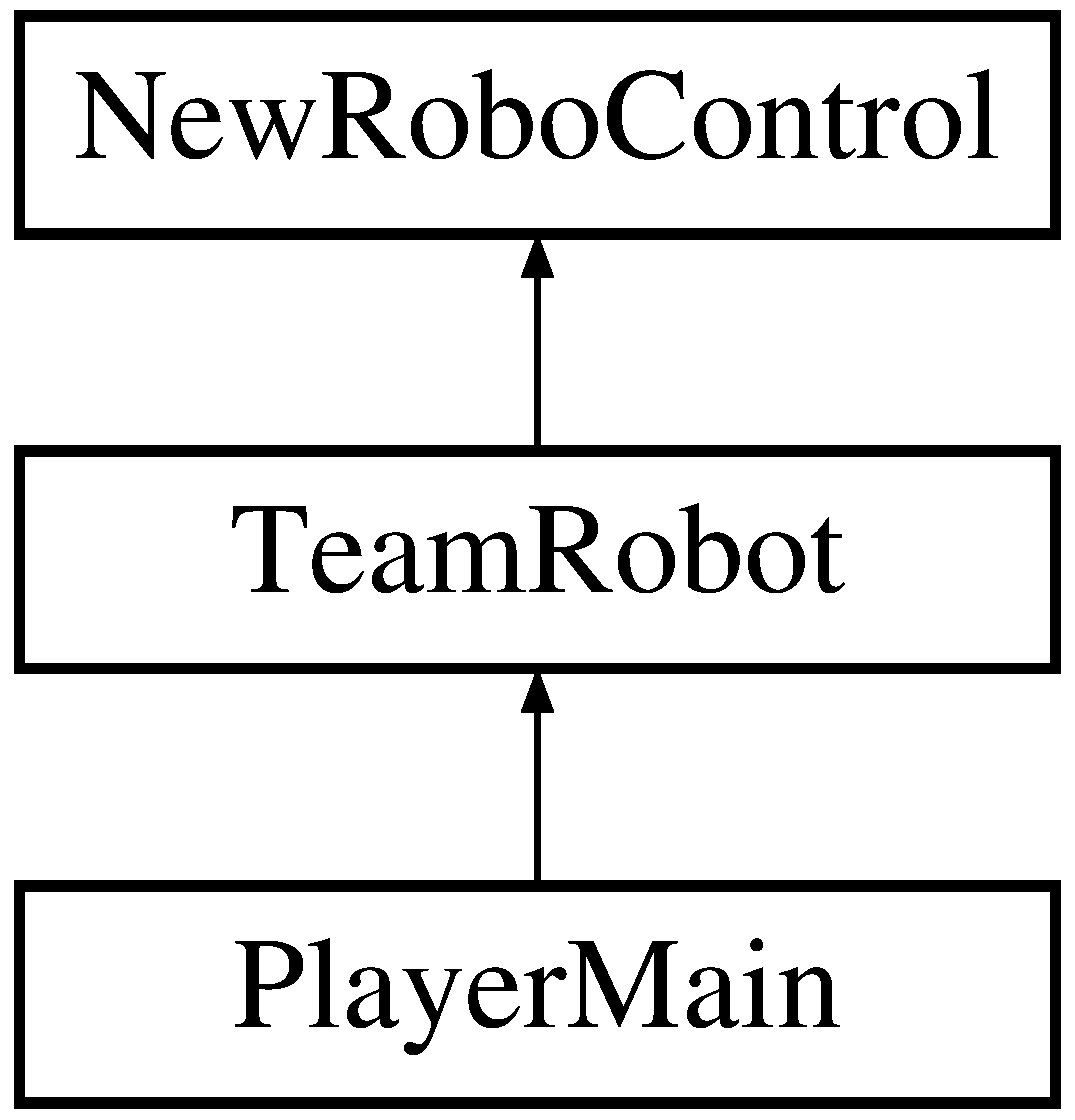
\includegraphics[height=3cm]{classPlayerMain}
\end{center}
\end{figure}
\subsection*{Public Types}
\begin{DoxyCompactItemize}
\item 
enum \hyperlink{classPlayerMain_af07f952a547b2902a452c1413f26dae2}{ActionPlayerMain} \{ \par
\hyperlink{classPlayerMain_af07f952a547b2902a452c1413f26dae2ad110267c0dfd47655250b6e11cb333ed}{GO\_\-TO\_\-DEF\_\-POS}, 
\hyperlink{classPlayerMain_af07f952a547b2902a452c1413f26dae2a3bfe9a85c58f83e457c2515fab072d03}{KICK\_\-PENALTY}, 
\hyperlink{classPlayerMain_af07f952a547b2902a452c1413f26dae2aa3a0ef85cf87cfe01eb07e7d72e959cd}{KICK\_\-OFF}, 
\hyperlink{classPlayerMain_af07f952a547b2902a452c1413f26dae2a182faa57b0ea5f67cd916a9261df12dc}{STOP}, 
\par
\hyperlink{classPlayerMain_af07f952a547b2902a452c1413f26dae2a19eca8a0a0720f6c698f344b4e6ffb72}{FOLLOWPATH}
 \}
\end{DoxyCompactItemize}
\subsection*{Public Member Functions}
\begin{DoxyCompactItemize}
\item 
\hyperlink{classPlayerMain_a12957aeecc6902370f03ff2ffbb0551d}{PlayerMain} (RTDBConn \&DBC, const int deviceNr, const \hyperlink{classCoordinatesCalibrer}{CoordinatesCalibrer} $\ast$c, RawBall $\ast$b, \hyperlink{classBallMonitor}{BallMonitor} $\ast$ballPm, \hyperlink{classRefereeDisplay}{RefereeDisplay} $\ast$display=NULL)
\item 
void \hyperlink{classPlayerMain_a8f0320189df15529662c7f16d2f74084}{setNextCmd} (const \hyperlink{structInterpreter_1_1GameData}{Interpreter::GameData} \&info)
\item 
void \hyperlink{classPlayerMain_a5c4af159392663660f91809052422945}{setCmdParam} (const \hyperlink{classInterpreter}{Interpreter} \&interpreter)
\item 
void \hyperlink{classPlayerMain_af12a95c226ce973056681a138b55fb6c}{performCmd} (const \hyperlink{structInterpreter_1_1GameData}{Interpreter::GameData} \&info)
\end{DoxyCompactItemize}
\subsection*{Private Member Functions}
\begin{DoxyCompactItemize}
\item 
void \hyperlink{classPlayerMain_a978b3ce16f5d8e5d1cb9ef70f387227e}{AddObstacleForFormation} (const \hyperlink{structInterpreter_1_1GameData}{Interpreter::GameData} \&info)
\item 
void \hyperlink{classPlayerMain_a64e1d5734e07cfa82b2571aa11bb4f9d}{defend\_\-p2} (void)
\end{DoxyCompactItemize}
\subsection*{Private Attributes}
\begin{DoxyCompactItemize}
\item 
\hyperlink{classPlayerMain_af07f952a547b2902a452c1413f26dae2}{ActionPlayerMain} \hyperlink{classPlayerMain_a038f8616ec79dd26bae8039b6ada8321}{m\_\-nextCmd}
\item 
\hyperlink{classBallMonitor}{BallMonitor} $\ast$ \hyperlink{classPlayerMain_aea071084f1a844ceafac3621ffb5c320}{m\_\-ballpm}
\item 
const \hyperlink{classNewRoboControl}{NewRoboControl} $\ast$ \hyperlink{classPlayerMain_a020813a869e52dc7368ba9216b10e3d8}{m\_\-otherRobots} \mbox{[}5\mbox{]}
\item 
Position \hyperlink{classPlayerMain_a859b462c123135acc3ad88b092429611}{m\_\-defendp2}
\end{DoxyCompactItemize}


\subsection{Member Enumeration Documentation}
\hypertarget{classPlayerMain_af07f952a547b2902a452c1413f26dae2}{
\index{PlayerMain@{PlayerMain}!ActionPlayerMain@{ActionPlayerMain}}
\index{ActionPlayerMain@{ActionPlayerMain}!PlayerMain@{PlayerMain}}
\subsubsection[{ActionPlayerMain}]{\setlength{\rightskip}{0pt plus 5cm}enum {\bf PlayerMain::ActionPlayerMain}}}
\label{classPlayerMain_af07f952a547b2902a452c1413f26dae2}
\begin{Desc}
\item[Enumerator: ]\par
\begin{description}
\index{GO\_\-TO\_\-DEF\_\-POS@{GO\_\-TO\_\-DEF\_\-POS}!PlayerMain@{PlayerMain}}\index{PlayerMain@{PlayerMain}!GO\_\-TO\_\-DEF\_\-POS@{GO\_\-TO\_\-DEF\_\-POS}}\item[{\em 
\hypertarget{classPlayerMain_af07f952a547b2902a452c1413f26dae2ad110267c0dfd47655250b6e11cb333ed}{
GO\_\-TO\_\-DEF\_\-POS}
\label{classPlayerMain_af07f952a547b2902a452c1413f26dae2ad110267c0dfd47655250b6e11cb333ed}
}]TODO \index{KICK\_\-PENALTY@{KICK\_\-PENALTY}!PlayerMain@{PlayerMain}}\index{PlayerMain@{PlayerMain}!KICK\_\-PENALTY@{KICK\_\-PENALTY}}\item[{\em 
\hypertarget{classPlayerMain_af07f952a547b2902a452c1413f26dae2a3bfe9a85c58f83e457c2515fab072d03}{
KICK\_\-PENALTY}
\label{classPlayerMain_af07f952a547b2902a452c1413f26dae2a3bfe9a85c58f83e457c2515fab072d03}
}]TODO \index{KICK\_\-OFF@{KICK\_\-OFF}!PlayerMain@{PlayerMain}}\index{PlayerMain@{PlayerMain}!KICK\_\-OFF@{KICK\_\-OFF}}\item[{\em 
\hypertarget{classPlayerMain_af07f952a547b2902a452c1413f26dae2aa3a0ef85cf87cfe01eb07e7d72e959cd}{
KICK\_\-OFF}
\label{classPlayerMain_af07f952a547b2902a452c1413f26dae2aa3a0ef85cf87cfe01eb07e7d72e959cd}
}]TODO \index{STOP@{STOP}!PlayerMain@{PlayerMain}}\index{PlayerMain@{PlayerMain}!STOP@{STOP}}\item[{\em 
\hypertarget{classPlayerMain_af07f952a547b2902a452c1413f26dae2a182faa57b0ea5f67cd916a9261df12dc}{
STOP}
\label{classPlayerMain_af07f952a547b2902a452c1413f26dae2a182faa57b0ea5f67cd916a9261df12dc}
}]TODO \index{FOLLOWPATH@{FOLLOWPATH}!PlayerMain@{PlayerMain}}\index{PlayerMain@{PlayerMain}!FOLLOWPATH@{FOLLOWPATH}}\item[{\em 
\hypertarget{classPlayerMain_af07f952a547b2902a452c1413f26dae2a19eca8a0a0720f6c698f344b4e6ffb72}{
FOLLOWPATH}
\label{classPlayerMain_af07f952a547b2902a452c1413f26dae2a19eca8a0a0720f6c698f344b4e6ffb72}
}]TODO \end{description}
\end{Desc}



\subsection{Constructor \& Destructor Documentation}
\hypertarget{classPlayerMain_a12957aeecc6902370f03ff2ffbb0551d}{
\index{PlayerMain@{PlayerMain}!PlayerMain@{PlayerMain}}
\index{PlayerMain@{PlayerMain}!PlayerMain@{PlayerMain}}
\subsubsection[{PlayerMain}]{\setlength{\rightskip}{0pt plus 5cm}PlayerMain::PlayerMain (RTDBConn \& {\em DBC}, \/  const int {\em deviceNr}, \/  const {\bf CoordinatesCalibrer} $\ast$ {\em c}, \/  RawBall $\ast$ {\em b}, \/  {\bf BallMonitor} $\ast$ {\em ballPm}, \/  {\bf RefereeDisplay} $\ast$ {\em display} = {\ttfamily NULL})}}
\label{classPlayerMain_a12957aeecc6902370f03ff2ffbb0551d}

\begin{DoxyParams}{Parameters}
\item[{\em DBC}]\item[{\em deviceNr}]\item[{\em c}]\item[{\em b}]\item[{\em ballPm}]\item[{\em display}]\end{DoxyParams}


\subsection{Member Function Documentation}
\hypertarget{classPlayerMain_a978b3ce16f5d8e5d1cb9ef70f387227e}{
\index{PlayerMain@{PlayerMain}!AddObstacleForFormation@{AddObstacleForFormation}}
\index{AddObstacleForFormation@{AddObstacleForFormation}!PlayerMain@{PlayerMain}}
\subsubsection[{AddObstacleForFormation}]{\setlength{\rightskip}{0pt plus 5cm}void PlayerMain::AddObstacleForFormation (const {\bf Interpreter::GameData} \& {\em info})\hspace{0.3cm}{\ttfamily  \mbox{[}private, virtual\mbox{]}}}}
\label{classPlayerMain_a978b3ce16f5d8e5d1cb9ef70f387227e}

\begin{DoxyParams}{Parameters}
\item[{\em info}]\end{DoxyParams}


Implements \hyperlink{classTeamRobot_a71ec65db46db1ac511fe17b668d4f192}{TeamRobot}.

\hypertarget{classPlayerMain_a64e1d5734e07cfa82b2571aa11bb4f9d}{
\index{PlayerMain@{PlayerMain}!defend\_\-p2@{defend\_\-p2}}
\index{defend\_\-p2@{defend\_\-p2}!PlayerMain@{PlayerMain}}
\subsubsection[{defend\_\-p2}]{\setlength{\rightskip}{0pt plus 5cm}void PlayerMain::defend\_\-p2 (void)\hspace{0.3cm}{\ttfamily  \mbox{[}private\mbox{]}}}}
\label{classPlayerMain_a64e1d5734e07cfa82b2571aa11bb4f9d}
\hypertarget{classPlayerMain_af12a95c226ce973056681a138b55fb6c}{
\index{PlayerMain@{PlayerMain}!performCmd@{performCmd}}
\index{performCmd@{performCmd}!PlayerMain@{PlayerMain}}
\subsubsection[{performCmd}]{\setlength{\rightskip}{0pt plus 5cm}void PlayerMain::performCmd (const {\bf Interpreter::GameData} \& {\em info})\hspace{0.3cm}{\ttfamily  \mbox{[}virtual\mbox{]}}}}
\label{classPlayerMain_af12a95c226ce973056681a138b55fb6c}

\begin{DoxyParams}{Parameters}
\item[{\em info}]\end{DoxyParams}


Implements \hyperlink{classTeamRobot_a9b84df51ca16a7203fdb6498ea6741da}{TeamRobot}.

\hypertarget{classPlayerMain_a5c4af159392663660f91809052422945}{
\index{PlayerMain@{PlayerMain}!setCmdParam@{setCmdParam}}
\index{setCmdParam@{setCmdParam}!PlayerMain@{PlayerMain}}
\subsubsection[{setCmdParam}]{\setlength{\rightskip}{0pt plus 5cm}void PlayerMain::setCmdParam (const {\bf Interpreter} \& {\em interpreter})\hspace{0.3cm}{\ttfamily  \mbox{[}virtual\mbox{]}}}}
\label{classPlayerMain_a5c4af159392663660f91809052422945}

\begin{DoxyParams}{Parameters}
\item[{\em interpreter}]\end{DoxyParams}


Implements \hyperlink{classTeamRobot_a34c0fd6986c510d4025e5752b3c0e49a}{TeamRobot}.

\hypertarget{classPlayerMain_a8f0320189df15529662c7f16d2f74084}{
\index{PlayerMain@{PlayerMain}!setNextCmd@{setNextCmd}}
\index{setNextCmd@{setNextCmd}!PlayerMain@{PlayerMain}}
\subsubsection[{setNextCmd}]{\setlength{\rightskip}{0pt plus 5cm}void PlayerMain::setNextCmd (const {\bf Interpreter::GameData} \& {\em info})\hspace{0.3cm}{\ttfamily  \mbox{[}virtual\mbox{]}}}}
\label{classPlayerMain_a8f0320189df15529662c7f16d2f74084}

\begin{DoxyParams}{Parameters}
\item[{\em info}]\end{DoxyParams}


Implements \hyperlink{classTeamRobot_a65f9a2b7464dfac3f4a0336810cf574f}{TeamRobot}.



\subsection{Member Data Documentation}
\hypertarget{classPlayerMain_aea071084f1a844ceafac3621ffb5c320}{
\index{PlayerMain@{PlayerMain}!m\_\-ballpm@{m\_\-ballpm}}
\index{m\_\-ballpm@{m\_\-ballpm}!PlayerMain@{PlayerMain}}
\subsubsection[{m\_\-ballpm}]{\setlength{\rightskip}{0pt plus 5cm}{\bf BallMonitor}$\ast$ {\bf PlayerMain::m\_\-ballpm}\hspace{0.3cm}{\ttfamily  \mbox{[}private\mbox{]}}}}
\label{classPlayerMain_aea071084f1a844ceafac3621ffb5c320}
TODO \hypertarget{classPlayerMain_a859b462c123135acc3ad88b092429611}{
\index{PlayerMain@{PlayerMain}!m\_\-defendp2@{m\_\-defendp2}}
\index{m\_\-defendp2@{m\_\-defendp2}!PlayerMain@{PlayerMain}}
\subsubsection[{m\_\-defendp2}]{\setlength{\rightskip}{0pt plus 5cm}Position {\bf PlayerMain::m\_\-defendp2}\hspace{0.3cm}{\ttfamily  \mbox{[}private\mbox{]}}}}
\label{classPlayerMain_a859b462c123135acc3ad88b092429611}
TODO \hypertarget{classPlayerMain_a038f8616ec79dd26bae8039b6ada8321}{
\index{PlayerMain@{PlayerMain}!m\_\-nextCmd@{m\_\-nextCmd}}
\index{m\_\-nextCmd@{m\_\-nextCmd}!PlayerMain@{PlayerMain}}
\subsubsection[{m\_\-nextCmd}]{\setlength{\rightskip}{0pt plus 5cm}{\bf ActionPlayerMain} {\bf PlayerMain::m\_\-nextCmd}\hspace{0.3cm}{\ttfamily  \mbox{[}private\mbox{]}}}}
\label{classPlayerMain_a038f8616ec79dd26bae8039b6ada8321}
TODO \hypertarget{classPlayerMain_a020813a869e52dc7368ba9216b10e3d8}{
\index{PlayerMain@{PlayerMain}!m\_\-otherRobots@{m\_\-otherRobots}}
\index{m\_\-otherRobots@{m\_\-otherRobots}!PlayerMain@{PlayerMain}}
\subsubsection[{m\_\-otherRobots}]{\setlength{\rightskip}{0pt plus 5cm}const {\bf NewRoboControl}$\ast$ {\bf PlayerMain::m\_\-otherRobots}\mbox{[}5\mbox{]}\hspace{0.3cm}{\ttfamily  \mbox{[}private\mbox{]}}}}
\label{classPlayerMain_a020813a869e52dc7368ba9216b10e3d8}
TODO 

The documentation for this class was generated from the following files:\begin{DoxyCompactItemize}
\item 
src/\hyperlink{playermain_8h}{playermain.h}\item 
src/\hyperlink{playermain_8cpp}{playermain.cpp}\end{DoxyCompactItemize}

\hypertarget{classPlayerTwo}{
\section{PlayerTwo Class Reference}
\label{classPlayerTwo}\index{PlayerTwo@{PlayerTwo}}
}


Child class of \hyperlink{classTeamRobot}{TeamRobot} which describes the second player.  




{\ttfamily \#include $<$playertwo.h$>$}



Inheritance diagram for PlayerTwo:\nopagebreak
\begin{figure}[H]
\begin{center}
\leavevmode
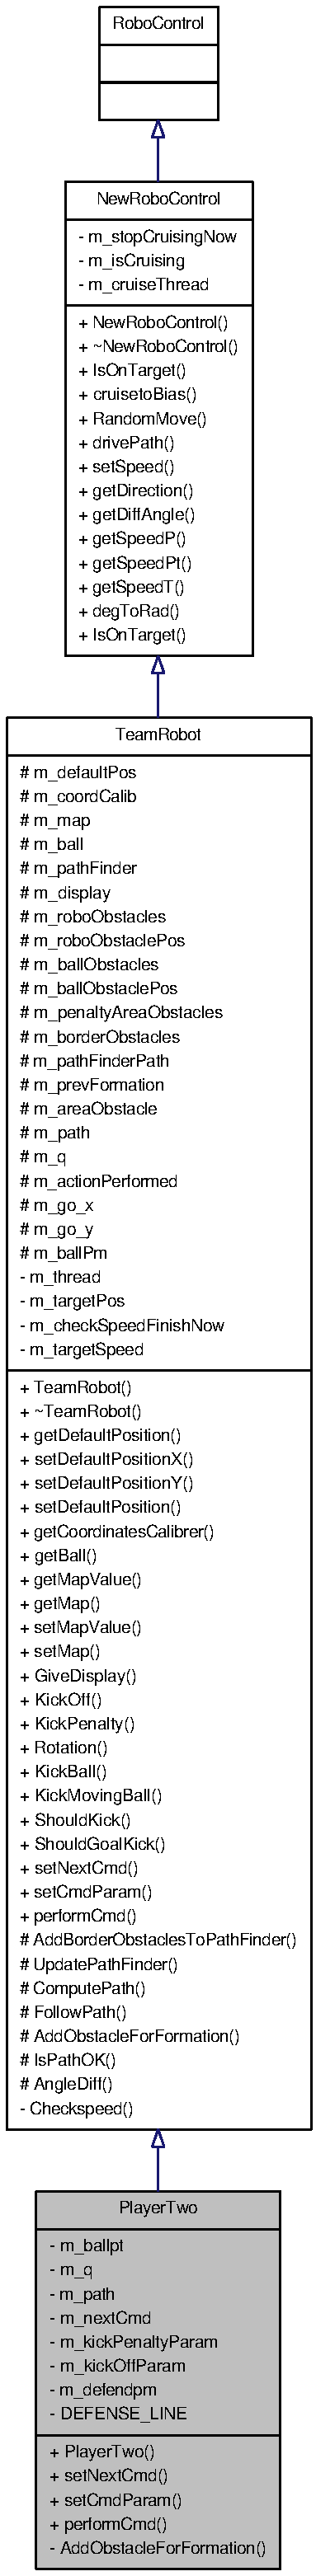
\includegraphics[height=400pt]{classPlayerTwo__inherit__graph}
\end{center}
\end{figure}
\subsection*{Classes}
\begin{DoxyCompactItemize}
\item 
struct \hyperlink{structPlayerTwo_1_1KickParam}{KickParam}
\end{DoxyCompactItemize}
\subsection*{Public Types}
\begin{DoxyCompactItemize}
\item 
enum \hyperlink{classPlayerTwo_a6dd2b1afb179fe02b677dd71ec5703d2}{ActionPlayerTwo} \{ \hyperlink{classPlayerTwo_a6dd2b1afb179fe02b677dd71ec5703d2a1ee0927d53a79a9c07f3e8347b65ec6e}{GO\_\-TO\_\-DEF\_\-POS}, 
\hyperlink{classPlayerTwo_a6dd2b1afb179fe02b677dd71ec5703d2abd5fef2f14d18f78f33c6e946f1c9cd7}{FOLLOWPATH}, 
\hyperlink{classPlayerTwo_a6dd2b1afb179fe02b677dd71ec5703d2aebb0cbac0bcb8fb7439a980dcc792638}{STOP}, 
\hyperlink{classPlayerTwo_a6dd2b1afb179fe02b677dd71ec5703d2a891b5407c8423ecb7d65df3a7da9b334}{DEFENSE}
 \}
\end{DoxyCompactItemize}
\subsection*{Public Member Functions}
\begin{DoxyCompactItemize}
\item 
\hyperlink{classPlayerTwo_ac69719e70c78f7dffa36300f833955b1}{PlayerTwo} (RTDBConn \&DBC, const int deviceNr, const \hyperlink{classCoordinatesCalibrer}{CoordinatesCalibrer} $\ast$coordCalib, RawBall $\ast$, \hyperlink{classBallMonitor}{BallMonitor} $\ast$ballPm, \hyperlink{classRefereeDisplay}{RefereeDisplay} $\ast$display=NULL)
\begin{DoxyCompactList}\small\item\em Constructor of \hyperlink{classPlayerTwo}{PlayerTwo} class. \item\end{DoxyCompactList}\item 
void \hyperlink{classPlayerTwo_a7ac9a9a4f1dedee2006e6a0c79f37c0c}{setNextCmd} (const \hyperlink{structInterpreter_1_1GameData}{Interpreter::GameData} \&info)
\begin{DoxyCompactList}\small\item\em Set next Command for \hyperlink{classPlayerTwo}{PlayerTwo}, depending on the command of \hyperlink{classInterpreter}{Interpreter} a case (strategy) is selected. \item\end{DoxyCompactList}\item 
void \hyperlink{classPlayerTwo_aa0294cf24297f66ffd92f1a250794340}{setCmdParam} (const \hyperlink{classInterpreter}{Interpreter} \&interpreter)
\begin{DoxyCompactList}\small\item\em this function sets the value of parameters depending on the selected strategy \item\end{DoxyCompactList}\item 
void \hyperlink{classPlayerTwo_a56d794b718c60092a324f312b8333eb9}{performCmd} (const \hyperlink{structInterpreter_1_1GameData}{Interpreter::GameData} \&info)
\begin{DoxyCompactList}\small\item\em the robot performs the command based on selected strategy \item\end{DoxyCompactList}\end{DoxyCompactItemize}
\subsection*{Private Member Functions}
\begin{DoxyCompactItemize}
\item 
void \hyperlink{classPlayerTwo_a9e3341541658f54a2dfb0491a774b4d4}{AddObstacleForFormation} (const \hyperlink{structInterpreter_1_1GameData}{Interpreter::GameData} \&info)
\begin{DoxyCompactList}\small\item\em in different play strategy, the robots are supposed to move only in certain area. This function is used to limit the movement of the robots \item\end{DoxyCompactList}\end{DoxyCompactItemize}
\subsection*{Private Attributes}
\begin{DoxyCompactItemize}
\item 
\hyperlink{classBallMonitor}{BallMonitor} $\ast$ \hyperlink{classPlayerTwo_a14f2fe35deb15d4d45208273a51ec7eb}{m\_\-ballpt}
\item 
queue$<$ int $>$ \hyperlink{classPlayerTwo_ac2f70709bd48ad9f5c2435cbff1e65b3}{m\_\-q}
\item 
string \hyperlink{classPlayerTwo_af9880885ced53351b52dcc949f6df162}{m\_\-path}
\item 
\hyperlink{classPlayerTwo_a6dd2b1afb179fe02b677dd71ec5703d2}{ActionPlayerTwo} \hyperlink{classPlayerTwo_a35bab8a32976849cd72828a1a1fe8504}{m\_\-nextCmd}
\item 
\hyperlink{structPlayerTwo_1_1KickParam}{KickParam} \hyperlink{classPlayerTwo_ac0b6376133a18b87e4fa14036a32f0ff}{m\_\-kickPenaltyParam}
\item 
Position \hyperlink{classPlayerTwo_af294f3bef80e0df881b4452c1272376a}{m\_\-kickOffParam}
\item 
Position \hyperlink{classPlayerTwo_aa6b42d687884c55d1dd30034e7952605}{m\_\-defendpm}
\end{DoxyCompactItemize}
\subsection*{Static Private Attributes}
\begin{DoxyCompactItemize}
\item 
static const double \hyperlink{classPlayerTwo_a86e1752bf84fab5d093f93633d3e51da}{DEFENSE\_\-LINE} = 0.75
\end{DoxyCompactItemize}


\subsection{Detailed Description}
Child class of \hyperlink{classTeamRobot}{TeamRobot} which describes the second player. The game behavior of the second player is slightly different from its brother \hyperlink{classPlayerMain}{player main}. 

\subsection{Member Enumeration Documentation}
\hypertarget{classPlayerTwo_a6dd2b1afb179fe02b677dd71ec5703d2}{
\index{PlayerTwo@{PlayerTwo}!ActionPlayerTwo@{ActionPlayerTwo}}
\index{ActionPlayerTwo@{ActionPlayerTwo}!PlayerTwo@{PlayerTwo}}
\subsubsection[{ActionPlayerTwo}]{\setlength{\rightskip}{0pt plus 5cm}enum {\bf PlayerTwo::ActionPlayerTwo}}}
\label{classPlayerTwo_a6dd2b1afb179fe02b677dd71ec5703d2}
\begin{Desc}
\item[Enumerator: ]\par
\begin{description}
\index{GO\_\-TO\_\-DEF\_\-POS@{GO\_\-TO\_\-DEF\_\-POS}!PlayerTwo@{PlayerTwo}}\index{PlayerTwo@{PlayerTwo}!GO\_\-TO\_\-DEF\_\-POS@{GO\_\-TO\_\-DEF\_\-POS}}\item[{\em 
\hypertarget{classPlayerTwo_a6dd2b1afb179fe02b677dd71ec5703d2a1ee0927d53a79a9c07f3e8347b65ec6e}{
GO\_\-TO\_\-DEF\_\-POS}
\label{classPlayerTwo_a6dd2b1afb179fe02b677dd71ec5703d2a1ee0927d53a79a9c07f3e8347b65ec6e}
}]TODO \index{FOLLOWPATH@{FOLLOWPATH}!PlayerTwo@{PlayerTwo}}\index{PlayerTwo@{PlayerTwo}!FOLLOWPATH@{FOLLOWPATH}}\item[{\em 
\hypertarget{classPlayerTwo_a6dd2b1afb179fe02b677dd71ec5703d2abd5fef2f14d18f78f33c6e946f1c9cd7}{
FOLLOWPATH}
\label{classPlayerTwo_a6dd2b1afb179fe02b677dd71ec5703d2abd5fef2f14d18f78f33c6e946f1c9cd7}
}]TODO \index{STOP@{STOP}!PlayerTwo@{PlayerTwo}}\index{PlayerTwo@{PlayerTwo}!STOP@{STOP}}\item[{\em 
\hypertarget{classPlayerTwo_a6dd2b1afb179fe02b677dd71ec5703d2aebb0cbac0bcb8fb7439a980dcc792638}{
STOP}
\label{classPlayerTwo_a6dd2b1afb179fe02b677dd71ec5703d2aebb0cbac0bcb8fb7439a980dcc792638}
}]TODO \index{DEFENSE@{DEFENSE}!PlayerTwo@{PlayerTwo}}\index{PlayerTwo@{PlayerTwo}!DEFENSE@{DEFENSE}}\item[{\em 
\hypertarget{classPlayerTwo_a6dd2b1afb179fe02b677dd71ec5703d2a891b5407c8423ecb7d65df3a7da9b334}{
DEFENSE}
\label{classPlayerTwo_a6dd2b1afb179fe02b677dd71ec5703d2a891b5407c8423ecb7d65df3a7da9b334}
}]TODO \end{description}
\end{Desc}



\subsection{Constructor \& Destructor Documentation}
\hypertarget{classPlayerTwo_ac69719e70c78f7dffa36300f833955b1}{
\index{PlayerTwo@{PlayerTwo}!PlayerTwo@{PlayerTwo}}
\index{PlayerTwo@{PlayerTwo}!PlayerTwo@{PlayerTwo}}
\subsubsection[{PlayerTwo}]{\setlength{\rightskip}{0pt plus 5cm}PlayerTwo::PlayerTwo (RTDBConn \& {\em DBC}, \/  const int {\em deviceNr}, \/  const {\bf CoordinatesCalibrer} $\ast$ {\em coordCalib}, \/  RawBall $\ast$ {\em b}, \/  {\bf BallMonitor} $\ast$ {\em ballPm}, \/  {\bf RefereeDisplay} $\ast$ {\em display} = {\ttfamily NULL})}}
\label{classPlayerTwo_ac69719e70c78f7dffa36300f833955b1}


Constructor of \hyperlink{classPlayerTwo}{PlayerTwo} class. 


\begin{DoxyParams}{Parameters}
\item[{\em DBC}]Database connexion \item[{\em deviceNr}]Number of the robot \item[{\em coordCalib}]Coordinates calibrator \item[{\em b}]Ball data \item[{\em ballPm}]Monitoring the ball \item[{\em display}]Display paths, robots ball \end{DoxyParams}


\subsection{Member Function Documentation}
\hypertarget{classPlayerTwo_a9e3341541658f54a2dfb0491a774b4d4}{
\index{PlayerTwo@{PlayerTwo}!AddObstacleForFormation@{AddObstacleForFormation}}
\index{AddObstacleForFormation@{AddObstacleForFormation}!PlayerTwo@{PlayerTwo}}
\subsubsection[{AddObstacleForFormation}]{\setlength{\rightskip}{0pt plus 5cm}void PlayerTwo::AddObstacleForFormation (const {\bf Interpreter::GameData} \& {\em info})\hspace{0.3cm}{\ttfamily  \mbox{[}private, virtual\mbox{]}}}}
\label{classPlayerTwo_a9e3341541658f54a2dfb0491a774b4d4}


in different play strategy, the robots are supposed to move only in certain area. This function is used to limit the movement of the robots 


\begin{DoxyParams}{Parameters}
\item[{\em info}]info is the current playmode and situation(score etc.) from referee \end{DoxyParams}


Implements \hyperlink{classTeamRobot_a71ec65db46db1ac511fe17b668d4f192}{TeamRobot}.

\hypertarget{classPlayerTwo_a56d794b718c60092a324f312b8333eb9}{
\index{PlayerTwo@{PlayerTwo}!performCmd@{performCmd}}
\index{performCmd@{performCmd}!PlayerTwo@{PlayerTwo}}
\subsubsection[{performCmd}]{\setlength{\rightskip}{0pt plus 5cm}void PlayerTwo::performCmd (const {\bf Interpreter::GameData} \& {\em info})\hspace{0.3cm}{\ttfamily  \mbox{[}virtual\mbox{]}}}}
\label{classPlayerTwo_a56d794b718c60092a324f312b8333eb9}


the robot performs the command based on selected strategy 


\begin{DoxyParams}{Parameters}
\item[{\em info}]Referee informations needed for side information \end{DoxyParams}


Implements \hyperlink{classTeamRobot_a9b84df51ca16a7203fdb6498ea6741da}{TeamRobot}.

\hypertarget{classPlayerTwo_aa0294cf24297f66ffd92f1a250794340}{
\index{PlayerTwo@{PlayerTwo}!setCmdParam@{setCmdParam}}
\index{setCmdParam@{setCmdParam}!PlayerTwo@{PlayerTwo}}
\subsubsection[{setCmdParam}]{\setlength{\rightskip}{0pt plus 5cm}void PlayerTwo::setCmdParam (const {\bf Interpreter} \& {\em interpreter})\hspace{0.3cm}{\ttfamily  \mbox{[}virtual\mbox{]}}}}
\label{classPlayerTwo_aa0294cf24297f66ffd92f1a250794340}


this function sets the value of parameters depending on the selected strategy 


\begin{DoxyParams}{Parameters}
\item[{\em interpreter}]is pointer to the \hyperlink{classInterpreter}{Interpreter}, needed for side informations \end{DoxyParams}


Implements \hyperlink{classTeamRobot_a34c0fd6986c510d4025e5752b3c0e49a}{TeamRobot}.

\hypertarget{classPlayerTwo_a7ac9a9a4f1dedee2006e6a0c79f37c0c}{
\index{PlayerTwo@{PlayerTwo}!setNextCmd@{setNextCmd}}
\index{setNextCmd@{setNextCmd}!PlayerTwo@{PlayerTwo}}
\subsubsection[{setNextCmd}]{\setlength{\rightskip}{0pt plus 5cm}void PlayerTwo::setNextCmd (const {\bf Interpreter::GameData} \& {\em info})\hspace{0.3cm}{\ttfamily  \mbox{[}virtual\mbox{]}}}}
\label{classPlayerTwo_a7ac9a9a4f1dedee2006e6a0c79f37c0c}


Set next Command for \hyperlink{classPlayerTwo}{PlayerTwo}, depending on the command of \hyperlink{classInterpreter}{Interpreter} a case (strategy) is selected. 


\begin{DoxyParams}{Parameters}
\item[{\em info}]Actual playmode given by \hyperlink{classInterpreter}{Interpreter} \end{DoxyParams}


Implements \hyperlink{classTeamRobot_a65f9a2b7464dfac3f4a0336810cf574f}{TeamRobot}.



\subsection{Member Data Documentation}
\hypertarget{classPlayerTwo_a86e1752bf84fab5d093f93633d3e51da}{
\index{PlayerTwo@{PlayerTwo}!DEFENSE\_\-LINE@{DEFENSE\_\-LINE}}
\index{DEFENSE\_\-LINE@{DEFENSE\_\-LINE}!PlayerTwo@{PlayerTwo}}
\subsubsection[{DEFENSE\_\-LINE}]{\setlength{\rightskip}{0pt plus 5cm}const double {\bf PlayerTwo::DEFENSE\_\-LINE} = 0.75\hspace{0.3cm}{\ttfamily  \mbox{[}static, private\mbox{]}}}}
\label{classPlayerTwo_a86e1752bf84fab5d093f93633d3e51da}
TODO \hypertarget{classPlayerTwo_a14f2fe35deb15d4d45208273a51ec7eb}{
\index{PlayerTwo@{PlayerTwo}!m\_\-ballpt@{m\_\-ballpt}}
\index{m\_\-ballpt@{m\_\-ballpt}!PlayerTwo@{PlayerTwo}}
\subsubsection[{m\_\-ballpt}]{\setlength{\rightskip}{0pt plus 5cm}{\bf BallMonitor}$\ast$ {\bf PlayerTwo::m\_\-ballpt}\hspace{0.3cm}{\ttfamily  \mbox{[}private\mbox{]}}}}
\label{classPlayerTwo_a14f2fe35deb15d4d45208273a51ec7eb}
TODO \hypertarget{classPlayerTwo_aa6b42d687884c55d1dd30034e7952605}{
\index{PlayerTwo@{PlayerTwo}!m\_\-defendpm@{m\_\-defendpm}}
\index{m\_\-defendpm@{m\_\-defendpm}!PlayerTwo@{PlayerTwo}}
\subsubsection[{m\_\-defendpm}]{\setlength{\rightskip}{0pt plus 5cm}Position {\bf PlayerTwo::m\_\-defendpm}\hspace{0.3cm}{\ttfamily  \mbox{[}private\mbox{]}}}}
\label{classPlayerTwo_aa6b42d687884c55d1dd30034e7952605}
TODO \hypertarget{classPlayerTwo_af294f3bef80e0df881b4452c1272376a}{
\index{PlayerTwo@{PlayerTwo}!m\_\-kickOffParam@{m\_\-kickOffParam}}
\index{m\_\-kickOffParam@{m\_\-kickOffParam}!PlayerTwo@{PlayerTwo}}
\subsubsection[{m\_\-kickOffParam}]{\setlength{\rightskip}{0pt plus 5cm}Position {\bf PlayerTwo::m\_\-kickOffParam}\hspace{0.3cm}{\ttfamily  \mbox{[}private\mbox{]}}}}
\label{classPlayerTwo_af294f3bef80e0df881b4452c1272376a}
TODO \hypertarget{classPlayerTwo_ac0b6376133a18b87e4fa14036a32f0ff}{
\index{PlayerTwo@{PlayerTwo}!m\_\-kickPenaltyParam@{m\_\-kickPenaltyParam}}
\index{m\_\-kickPenaltyParam@{m\_\-kickPenaltyParam}!PlayerTwo@{PlayerTwo}}
\subsubsection[{m\_\-kickPenaltyParam}]{\setlength{\rightskip}{0pt plus 5cm}{\bf KickParam} {\bf PlayerTwo::m\_\-kickPenaltyParam}\hspace{0.3cm}{\ttfamily  \mbox{[}private\mbox{]}}}}
\label{classPlayerTwo_ac0b6376133a18b87e4fa14036a32f0ff}
TODO \hypertarget{classPlayerTwo_a35bab8a32976849cd72828a1a1fe8504}{
\index{PlayerTwo@{PlayerTwo}!m\_\-nextCmd@{m\_\-nextCmd}}
\index{m\_\-nextCmd@{m\_\-nextCmd}!PlayerTwo@{PlayerTwo}}
\subsubsection[{m\_\-nextCmd}]{\setlength{\rightskip}{0pt plus 5cm}{\bf ActionPlayerTwo} {\bf PlayerTwo::m\_\-nextCmd}\hspace{0.3cm}{\ttfamily  \mbox{[}private\mbox{]}}}}
\label{classPlayerTwo_a35bab8a32976849cd72828a1a1fe8504}
TODO \hypertarget{classPlayerTwo_af9880885ced53351b52dcc949f6df162}{
\index{PlayerTwo@{PlayerTwo}!m\_\-path@{m\_\-path}}
\index{m\_\-path@{m\_\-path}!PlayerTwo@{PlayerTwo}}
\subsubsection[{m\_\-path}]{\setlength{\rightskip}{0pt plus 5cm}string {\bf PlayerTwo::m\_\-path}\hspace{0.3cm}{\ttfamily  \mbox{[}private\mbox{]}}}}
\label{classPlayerTwo_af9880885ced53351b52dcc949f6df162}
TODO 

Reimplemented from \hyperlink{classTeamRobot_af170b8d2e1b76b12f8cc83f6ec908e40}{TeamRobot}.

\hypertarget{classPlayerTwo_ac2f70709bd48ad9f5c2435cbff1e65b3}{
\index{PlayerTwo@{PlayerTwo}!m\_\-q@{m\_\-q}}
\index{m\_\-q@{m\_\-q}!PlayerTwo@{PlayerTwo}}
\subsubsection[{m\_\-q}]{\setlength{\rightskip}{0pt plus 5cm}queue$<$int$>$ {\bf PlayerTwo::m\_\-q}\hspace{0.3cm}{\ttfamily  \mbox{[}private\mbox{]}}}}
\label{classPlayerTwo_ac2f70709bd48ad9f5c2435cbff1e65b3}
TODO 

Reimplemented from \hyperlink{classTeamRobot_a982ed6b6964c5e8b94519ef91b52c468}{TeamRobot}.



The documentation for this class was generated from the following files:\begin{DoxyCompactItemize}
\item 
src/\hyperlink{playertwo_8h}{playertwo.h}\item 
src/\hyperlink{playertwo_8cpp}{playertwo.cpp}\end{DoxyCompactItemize}

\hypertarget{structInterpreter_1_1Point}{
\section{Interpreter::Point Struct Reference}
\label{structInterpreter_1_1Point}\index{Interpreter::Point@{Interpreter::Point}}
}


{\ttfamily \#include $<$interpreter.h$>$}

\subsection*{Public Attributes}
\begin{DoxyCompactItemize}
\item 
int \hyperlink{structInterpreter_1_1Point_adb600c47a8131eae82454d92e81e6956}{x}
\item 
int \hyperlink{structInterpreter_1_1Point_a61e3664bd27fa93316e4cb7ec5758c54}{y}
\end{DoxyCompactItemize}


\subsection{Member Data Documentation}
\hypertarget{structInterpreter_1_1Point_adb600c47a8131eae82454d92e81e6956}{
\index{Interpreter::Point@{Interpreter::Point}!x@{x}}
\index{x@{x}!Interpreter::Point@{Interpreter::Point}}
\subsubsection[{x}]{\setlength{\rightskip}{0pt plus 5cm}int {\bf Interpreter::Point::x}}}
\label{structInterpreter_1_1Point_adb600c47a8131eae82454d92e81e6956}
TODO \hypertarget{structInterpreter_1_1Point_a61e3664bd27fa93316e4cb7ec5758c54}{
\index{Interpreter::Point@{Interpreter::Point}!y@{y}}
\index{y@{y}!Interpreter::Point@{Interpreter::Point}}
\subsubsection[{y}]{\setlength{\rightskip}{0pt plus 5cm}int {\bf Interpreter::Point::y}}}
\label{structInterpreter_1_1Point_a61e3664bd27fa93316e4cb7ec5758c54}
TODO 

The documentation for this struct was generated from the following file:\begin{DoxyCompactItemize}
\item 
src/\hyperlink{interpreter_8h}{interpreter.h}\end{DoxyCompactItemize}

\hypertarget{structMatrix_1_1Point}{
\section{Matrix::Point Struct Reference}
\label{structMatrix_1_1Point}\index{Matrix::Point@{Matrix::Point}}
}


Structure used to describe a simple integer point.  




{\ttfamily \#include $<$matrix.h$>$}

\subsection*{Public Attributes}
\begin{DoxyCompactItemize}
\item 
int \hyperlink{structMatrix_1_1Point_a2b232ad12860c70ec725e7ddb3034a1e}{x}
\item 
int \hyperlink{structMatrix_1_1Point_aefcca947f63a8ed4d5de75b5e3ffd322}{y}
\end{DoxyCompactItemize}


\subsection{Detailed Description}
Structure used to describe a simple integer point. 

\subsection{Member Data Documentation}
\hypertarget{structMatrix_1_1Point_a2b232ad12860c70ec725e7ddb3034a1e}{
\index{Matrix::Point@{Matrix::Point}!x@{x}}
\index{x@{x}!Matrix::Point@{Matrix::Point}}
\subsubsection[{x}]{\setlength{\rightskip}{0pt plus 5cm}int {\bf Matrix::Point::x}}}
\label{structMatrix_1_1Point_a2b232ad12860c70ec725e7ddb3034a1e}
x coordinate \hypertarget{structMatrix_1_1Point_aefcca947f63a8ed4d5de75b5e3ffd322}{
\index{Matrix::Point@{Matrix::Point}!y@{y}}
\index{y@{y}!Matrix::Point@{Matrix::Point}}
\subsubsection[{y}]{\setlength{\rightskip}{0pt plus 5cm}int {\bf Matrix::Point::y}}}
\label{structMatrix_1_1Point_aefcca947f63a8ed4d5de75b5e3ffd322}
y coordinate 

The documentation for this struct was generated from the following file:\begin{DoxyCompactItemize}
\item 
src/\hyperlink{matrix_8h}{matrix.h}\end{DoxyCompactItemize}

\hypertarget{structPathFinder_1_1Point}{
\section{PathFinder::Point Struct Reference}
\label{structPathFinder_1_1Point}\index{PathFinder::Point@{PathFinder::Point}}
}


Structure to represent a point in the path finder.  




{\ttfamily \#include $<$pathfinder.h$>$}

\subsection*{Public Attributes}
\begin{DoxyCompactItemize}
\item 
double \hyperlink{structPathFinder_1_1Point_a1be04f9eff0baa49c0e079f203c485f1}{x}
\item 
double \hyperlink{structPathFinder_1_1Point_a4e29ec03f42f8c196500ed6482ff2c78}{y}
\item 
\hyperlink{classPathFinder_a792a34ce673309f873090141c3d96f1c}{PointsList} \hyperlink{structPathFinder_1_1Point_a8d0aee1e967e4a319b2cb78e116ec66f}{visMap}
\item 
double \hyperlink{structPathFinder_1_1Point_a56c732ebd9055f0f74fade3b63cfdd46}{score}
\item 
\hyperlink{structPathFinder_1_1Point}{Point} $\ast$ \hyperlink{structPathFinder_1_1Point_a838fc3da5494344ab8fcdd5e6fea6173}{prevPoint}
\end{DoxyCompactItemize}


\subsection{Detailed Description}
Structure to represent a point in the path finder. A point should always be created with the static method \hyperlink{classPathFinder_a457592f3579bbe0c0527360c2c8a928a}{PathFinder::CreatePoint()}. 

\subsection{Member Data Documentation}
\hypertarget{structPathFinder_1_1Point_a838fc3da5494344ab8fcdd5e6fea6173}{
\index{PathFinder::Point@{PathFinder::Point}!prevPoint@{prevPoint}}
\index{prevPoint@{prevPoint}!PathFinder::Point@{PathFinder::Point}}
\subsubsection[{prevPoint}]{\setlength{\rightskip}{0pt plus 5cm}{\bf Point}$\ast$ {\bf PathFinder::Point::prevPoint}}}
\label{structPathFinder_1_1Point_a838fc3da5494344ab8fcdd5e6fea6173}
The parent of the point when excuting the Dijkstra's Algorithm. \hypertarget{structPathFinder_1_1Point_a56c732ebd9055f0f74fade3b63cfdd46}{
\index{PathFinder::Point@{PathFinder::Point}!score@{score}}
\index{score@{score}!PathFinder::Point@{PathFinder::Point}}
\subsubsection[{score}]{\setlength{\rightskip}{0pt plus 5cm}double {\bf PathFinder::Point::score}}}
\label{structPathFinder_1_1Point_a56c732ebd9055f0f74fade3b63cfdd46}
The score of the point when executing the Dijkstra's Algorithm. \hypertarget{structPathFinder_1_1Point_a8d0aee1e967e4a319b2cb78e116ec66f}{
\index{PathFinder::Point@{PathFinder::Point}!visMap@{visMap}}
\index{visMap@{visMap}!PathFinder::Point@{PathFinder::Point}}
\subsubsection[{visMap}]{\setlength{\rightskip}{0pt plus 5cm}{\bf PointsList} {\bf PathFinder::Point::visMap}}}
\label{structPathFinder_1_1Point_a8d0aee1e967e4a319b2cb78e116ec66f}
List of points which are visible from this point. \hypertarget{structPathFinder_1_1Point_a1be04f9eff0baa49c0e079f203c485f1}{
\index{PathFinder::Point@{PathFinder::Point}!x@{x}}
\index{x@{x}!PathFinder::Point@{PathFinder::Point}}
\subsubsection[{x}]{\setlength{\rightskip}{0pt plus 5cm}double {\bf PathFinder::Point::x}}}
\label{structPathFinder_1_1Point_a1be04f9eff0baa49c0e079f203c485f1}
x coordinate of the point. \hypertarget{structPathFinder_1_1Point_a4e29ec03f42f8c196500ed6482ff2c78}{
\index{PathFinder::Point@{PathFinder::Point}!y@{y}}
\index{y@{y}!PathFinder::Point@{PathFinder::Point}}
\subsubsection[{y}]{\setlength{\rightskip}{0pt plus 5cm}double {\bf PathFinder::Point::y}}}
\label{structPathFinder_1_1Point_a4e29ec03f42f8c196500ed6482ff2c78}
y coordinate of the point. 

The documentation for this struct was generated from the following file:\begin{DoxyCompactItemize}
\item 
src/\hyperlink{pathfinder_8h}{pathfinder.h}\end{DoxyCompactItemize}

\hypertarget{structBallMonitor_1_1PosTime}{
\section{BallMonitor::PosTime Struct Reference}
\label{structBallMonitor_1_1PosTime}\index{BallMonitor::PosTime@{BallMonitor::PosTime}}
}


This structure contains the position of the ball and the given time.  




{\ttfamily \#include $<$ballmonitor.h$>$}

\subsection*{Public Attributes}
\begin{DoxyCompactItemize}
\item 
Position \hyperlink{structBallMonitor_1_1PosTime_ae049de4ada401c92ec560198e5947e59}{pos}
\item 
clock\_\-t \hyperlink{structBallMonitor_1_1PosTime_ae56e28b26f0d91d164d5bfe0b0644cb2}{time}
\end{DoxyCompactItemize}


\subsection{Detailed Description}
This structure contains the position of the ball and the given time. 

\subsection{Member Data Documentation}
\hypertarget{structBallMonitor_1_1PosTime_ae049de4ada401c92ec560198e5947e59}{
\index{BallMonitor::PosTime@{BallMonitor::PosTime}!pos@{pos}}
\index{pos@{pos}!BallMonitor::PosTime@{BallMonitor::PosTime}}
\subsubsection[{pos}]{\setlength{\rightskip}{0pt plus 5cm}Position {\bf BallMonitor::PosTime::pos}}}
\label{structBallMonitor_1_1PosTime_ae049de4ada401c92ec560198e5947e59}
Ball position \hypertarget{structBallMonitor_1_1PosTime_ae56e28b26f0d91d164d5bfe0b0644cb2}{
\index{BallMonitor::PosTime@{BallMonitor::PosTime}!time@{time}}
\index{time@{time}!BallMonitor::PosTime@{BallMonitor::PosTime}}
\subsubsection[{time}]{\setlength{\rightskip}{0pt plus 5cm}clock\_\-t {\bf BallMonitor::PosTime::time}}}
\label{structBallMonitor_1_1PosTime_ae56e28b26f0d91d164d5bfe0b0644cb2}
Time at which the position was registered 

The documentation for this struct was generated from the following file:\begin{DoxyCompactItemize}
\item 
src/\hyperlink{ballmonitor_8h}{ballmonitor.h}\end{DoxyCompactItemize}

\hypertarget{structPathFinder_1_1Rectangle}{
\section{PathFinder::Rectangle Struct Reference}
\label{structPathFinder_1_1Rectangle}\index{PathFinder::Rectangle@{PathFinder::Rectangle}}
}


Structure used to represent a horizontal rectangle.  


\subsection*{Public Attributes}
\begin{DoxyCompactItemize}
\item 
\hyperlink{structPathFinder_1_1Point}{Point} \hyperlink{structPathFinder_1_1Rectangle_a9702d191b5627d0588f4053ac671aecf}{ul}
\item 
\hyperlink{structPathFinder_1_1Point}{Point} \hyperlink{structPathFinder_1_1Rectangle_adec50e08ca85bd83d626ab4ccefd3258}{lr}
\end{DoxyCompactItemize}


\subsection{Detailed Description}
Structure used to represent a horizontal rectangle. 

\subsection{Member Data Documentation}
\hypertarget{structPathFinder_1_1Rectangle_adec50e08ca85bd83d626ab4ccefd3258}{
\index{PathFinder::Rectangle@{PathFinder::Rectangle}!lr@{lr}}
\index{lr@{lr}!PathFinder::Rectangle@{PathFinder::Rectangle}}
\subsubsection[{lr}]{\setlength{\rightskip}{0pt plus 5cm}{\bf Point} {\bf PathFinder::Rectangle::lr}}}
\label{structPathFinder_1_1Rectangle_adec50e08ca85bd83d626ab4ccefd3258}
The lower right corner of the rectangle. \hypertarget{structPathFinder_1_1Rectangle_a9702d191b5627d0588f4053ac671aecf}{
\index{PathFinder::Rectangle@{PathFinder::Rectangle}!ul@{ul}}
\index{ul@{ul}!PathFinder::Rectangle@{PathFinder::Rectangle}}
\subsubsection[{ul}]{\setlength{\rightskip}{0pt plus 5cm}{\bf Point} {\bf PathFinder::Rectangle::ul}}}
\label{structPathFinder_1_1Rectangle_a9702d191b5627d0588f4053ac671aecf}
The upper left corner of the rectangle. 

The documentation for this struct was generated from the following file:\begin{DoxyCompactItemize}
\item 
src/\hyperlink{pathfinder_8h}{pathfinder.h}\end{DoxyCompactItemize}

\hypertarget{classRefereeDisplay}{
\section{RefereeDisplay Class Reference}
\label{classRefereeDisplay}\index{RefereeDisplay@{RefereeDisplay}}
}


Class used to create a window and display visual information in it. Also implements a basic interface system.  




{\ttfamily \#include $<$refereedisplay.h$>$}

\subsection*{Public Member Functions}
\begin{DoxyCompactItemize}
\item 
\hyperlink{classRefereeDisplay_a8f7d4872a24b44b96a36a5bbf991f5d2}{RefereeDisplay} (\hyperlink{classBallMonitor}{BallMonitor} $\ast$ballMonitor, const \hyperlink{classCoordinatesCalibrer}{CoordinatesCalibrer} $\ast$coordCalibrer, int screenW=800, int screenH=600, \hyperlink{classNewRoboControl}{NewRoboControl} $\ast$$\ast$robots=NULL, const \hyperlink{classInterpreter}{Interpreter} $\ast$interpreter=NULL)
\begin{DoxyCompactList}\small\item\em Standard constructor. \item\end{DoxyCompactList}\item 
\hyperlink{classRefereeDisplay_a5a9191c0d7f937df62ea9544d9e38f3b}{$\sim$RefereeDisplay} ()
\begin{DoxyCompactList}\small\item\em Standard destructor. \item\end{DoxyCompactList}\item 
bool \hyperlink{classRefereeDisplay_a6b789ef1ca73c72556cf5051a8a2b5a6}{StartDisplay} (\hyperlink{classNewRoboControl}{NewRoboControl} $\ast$$\ast$robots=NULL, const \hyperlink{classInterpreter}{Interpreter} $\ast$interpreter=NULL, const \hyperlink{classMatrix}{Interpreter::Map} $\ast$map=NULL)
\begin{DoxyCompactList}\small\item\em Creates a window and launches a thread to keep it updated with the game data. \item\end{DoxyCompactList}\item 
bool \hyperlink{classRefereeDisplay_aafa710132ce88c4e6cb4d430baf26173}{StopDisplay} ()
\begin{DoxyCompactList}\small\item\em Destroys the display's window created by \hyperlink{classRefereeDisplay_a6b789ef1ca73c72556cf5051a8a2b5a6}{RefereeDisplay::StartDisplay()}. \item\end{DoxyCompactList}\item 
bool \hyperlink{classRefereeDisplay_a216bbade42b7c7694f69d73c35620fc6}{IsActive} () const 
\begin{DoxyCompactList}\small\item\em Tells if the window is created and active. \item\end{DoxyCompactList}\item 
void \hyperlink{classRefereeDisplay_a0ef334a53e0fde02da30460ed2fcbe06}{DisplayPathFinder} (\hyperlink{classPathFinder}{PathFinder} $\ast$pathFinder)
\begin{DoxyCompactList}\small\item\em Adds the world of the provided \hyperlink{classPathFinder}{path finder} to the display. \item\end{DoxyCompactList}\item 
void \hyperlink{classRefereeDisplay_ad7f07077e92fd46956bf1aa25715e414}{DisplayPath} (const \hyperlink{classPathFinder_a269aba09b7b3208092f67f2bc02cf63e}{PathFinder::Path} path)
\begin{DoxyCompactList}\small\item\em Adds a \hyperlink{classPathFinder_a269aba09b7b3208092f67f2bc02cf63e}{path} to the display. \item\end{DoxyCompactList}\end{DoxyCompactItemize}
\subsection*{Private Member Functions}
\begin{DoxyCompactItemize}
\item 
void \hyperlink{classRefereeDisplay_a9c18f26c62f9507f903ec9b29c1bfea8}{CreateMapDisplay} (const \hyperlink{classMatrix}{Interpreter::Map} $\ast$map)
\begin{DoxyCompactList}\small\item\em Creates an internal \hyperlink{classMapDisplay}{display} for the given \hyperlink{classInterpreter_a4c080f069f557cf92dfe803117a6ea53}{obstacles map}. \item\end{DoxyCompactList}\item 
void \hyperlink{classRefereeDisplay_ae40cc8040d1fe441a8f38fe2fc0b8974}{DisplayWeb} (const \hyperlink{structPathFinder_1_1ConvexPolygon}{PathFinder::ConvexPolygon} \&polygon, SDL\_\-Surface $\ast$screen)
\begin{DoxyCompactList}\small\item\em Displays the vertices links which are connected to the given \hyperlink{structPathFinder_1_1ConvexPolygon}{polygon} in the world of the \hyperlink{classPathFinder}{path finder} of the display, if any. \item\end{DoxyCompactList}\item 
SDL\_\-Rect \hyperlink{classRefereeDisplay_a56d7e17a5fb16cbe64fb7ef3e4f28af0}{PosToRect} (Position pos, int w=0, int h=0)
\begin{DoxyCompactList}\small\item\em Converts a NORMALIZED position (see \hyperlink{classCoordinatesCalibrer}{CoordinatesCalibrer} for more info) to screen coordinates. \item\end{DoxyCompactList}\item 
Position \hyperlink{classRefereeDisplay_a4abb9b85d92cbdd30fe6fd29a17c3767}{RectToPos} (SDL\_\-Rect rect)
\begin{DoxyCompactList}\small\item\em Converts screen coordinates to a normalized position (see \hyperlink{classCoordinatesCalibrer}{CoordinatesCalibrer} for more info). \item\end{DoxyCompactList}\item 
Position \hyperlink{classRefereeDisplay_afa7601bcd5b6361398f48f2fb1d6ead4}{GetBallPos} ()
\begin{DoxyCompactList}\small\item\em Gets the unnormalized position of the ball, extracted from the internal \hyperlink{classBallMonitor}{ball monitoring system} (provided in the \hyperlink{classRefereeDisplay_a8f7d4872a24b44b96a36a5bbf991f5d2}{constructor}). \item\end{DoxyCompactList}\end{DoxyCompactItemize}
\subsection*{Static Private Member Functions}
\begin{DoxyCompactItemize}
\item 
static void $\ast$ \hyperlink{classRefereeDisplay_a0aecfa7e27f573859a1bb037aca9693a}{RefDisplayFn} (void $\ast$data)
\begin{DoxyCompactList}\small\item\em Main display loop, designed to be launched in a separate thread. \item\end{DoxyCompactList}\end{DoxyCompactItemize}
\subsection*{Private Attributes}
\begin{DoxyCompactItemize}
\item 
bool \hyperlink{classRefereeDisplay_af3bb14682e53eef2d7d9e664f84e6ba1}{m\_\-keepGoing}
\item 
bool \hyperlink{classRefereeDisplay_a12bdb098bcf59351f55bc7beb922ac62}{m\_\-isDisplaying}
\item 
pthread\_\-t \hyperlink{classRefereeDisplay_aded3908927ad3726777ece4d52cf3ca2}{m\_\-displayThread}
\item 
int \hyperlink{classRefereeDisplay_aed7aa88d65bc9b4f79fe8dd2598a92e5}{m\_\-screenW}
\item 
int \hyperlink{classRefereeDisplay_a136af0a18d0eadffbcaa755fdf76e328}{m\_\-screenH}
\item 
\hyperlink{classNewRoboControl}{NewRoboControl} $\ast$ \hyperlink{classRefereeDisplay_a4a777a38327f96fe1e5c9051b6c3c38f}{m\_\-robots} \mbox{[}6\mbox{]}
\item 
const \hyperlink{classInterpreter}{Interpreter} $\ast$ \hyperlink{classRefereeDisplay_a510383c894f917032aadc71f1f31074f}{m\_\-interpreter}
\item 
eTeam \hyperlink{classRefereeDisplay_a02ec6cdc79904b4727553f6802c36d9e}{m\_\-team}
\item 
\hyperlink{classBallMonitor}{BallMonitor} $\ast$ \hyperlink{classRefereeDisplay_ab3a1d764a476c413ed1f19be2c9a1215}{m\_\-ballMonitor}
\item 
const \hyperlink{classCoordinatesCalibrer}{CoordinatesCalibrer} $\ast$ \hyperlink{classRefereeDisplay_a7be832637684b08b915a2ff3c6c0d9f2}{m\_\-coordCalibrer}
\item 
\hyperlink{classMapDisplay}{MapDisplay} $\ast$ \hyperlink{classRefereeDisplay_a07fda892af04771c6484160fb0e5585f}{m\_\-mapDisplay}
\item 
std::vector$<$ \hyperlink{structPathFinder_1_1Point}{PathFinder::Point} $>$ \hyperlink{classRefereeDisplay_a582b6bcc0204a2876b629e8ceebc8abd}{m\_\-path}
\item 
\hyperlink{classPathFinder}{PathFinder} $\ast$ \hyperlink{classRefereeDisplay_a0ccee8231a72e1a906dff856e072d5a0}{m\_\-pathFinder}
\item 
pthread\_\-mutex\_\-t \hyperlink{classRefereeDisplay_a2ec44bb3c993cb8e518a730153116da7}{m\_\-pathMutex}
\end{DoxyCompactItemize}


\subsection{Detailed Description}
Class used to create a window and display visual information in it. Also implements a basic interface system. 

\subsection{Constructor \& Destructor Documentation}
\hypertarget{classRefereeDisplay_a8f7d4872a24b44b96a36a5bbf991f5d2}{
\index{RefereeDisplay@{RefereeDisplay}!RefereeDisplay@{RefereeDisplay}}
\index{RefereeDisplay@{RefereeDisplay}!RefereeDisplay@{RefereeDisplay}}
\subsubsection[{RefereeDisplay}]{\setlength{\rightskip}{0pt plus 5cm}RefereeDisplay::RefereeDisplay ({\bf BallMonitor} $\ast$ {\em ballMonitor}, \/  const {\bf CoordinatesCalibrer} $\ast$ {\em coordCalibrer}, \/  int {\em screenW} = {\ttfamily 800}, \/  int {\em screenH} = {\ttfamily 600}, \/  {\bf NewRoboControl} $\ast$$\ast$ {\em robots} = {\ttfamily NULL}, \/  const {\bf Interpreter} $\ast$ {\em interpreter} = {\ttfamily NULL})}}
\label{classRefereeDisplay_a8f7d4872a24b44b96a36a5bbf991f5d2}


Standard constructor. 

Once the instance is created, you must call the \hyperlink{classRefereeDisplay_a6b789ef1ca73c72556cf5051a8a2b5a6}{RefereeDisplay::StartDisplay()} function to create the display's window. Once the window is created, you must call the \hyperlink{classRefereeDisplay_aafa710132ce88c4e6cb4d430baf26173}{RefereeDisplay::StopDisplay()} function to destroy it before destroying the object.


\begin{DoxyParams}{Parameters}
\item[{\em ballMonitor}]A ball monitoring system. The display uses it to display the ball. \item[{\em coordCalibrer}]A coordinates calibrator. \item[{\em screenW}]The width of the window you want, in pixels. \item[{\em screenH}]The height of the window you want, in pixels. \item[{\em robots}]An array containing the six robots. Can be NULL but in this case you will have to provide them when calling the \hyperlink{classRefereeDisplay_a6b789ef1ca73c72556cf5051a8a2b5a6}{RefereeDisplay::StartDisplay()} function. \item[{\em interpreter}]The interpreter ruling the game. Can be NULL but in this case you will have to provide it when calling the \hyperlink{classRefereeDisplay_a6b789ef1ca73c72556cf5051a8a2b5a6}{RefereeDisplay::StartDisplay()} function. \end{DoxyParams}
\hypertarget{classRefereeDisplay_a5a9191c0d7f937df62ea9544d9e38f3b}{
\index{RefereeDisplay@{RefereeDisplay}!$\sim$RefereeDisplay@{$\sim$RefereeDisplay}}
\index{$\sim$RefereeDisplay@{$\sim$RefereeDisplay}!RefereeDisplay@{RefereeDisplay}}
\subsubsection[{$\sim$RefereeDisplay}]{\setlength{\rightskip}{0pt plus 5cm}RefereeDisplay::$\sim$RefereeDisplay ()}}
\label{classRefereeDisplay_a5a9191c0d7f937df62ea9544d9e38f3b}


Standard destructor. 

This desctructor does not close the window and does not free the memory associated with the window. Consequently, the \hyperlink{classRefereeDisplay_aafa710132ce88c4e6cb4d430baf26173}{RefereeDisplay::StopDisplay()} function must be called before the destructor, if a window was created. 

\subsection{Member Function Documentation}
\hypertarget{classRefereeDisplay_a9c18f26c62f9507f903ec9b29c1bfea8}{
\index{RefereeDisplay@{RefereeDisplay}!CreateMapDisplay@{CreateMapDisplay}}
\index{CreateMapDisplay@{CreateMapDisplay}!RefereeDisplay@{RefereeDisplay}}
\subsubsection[{CreateMapDisplay}]{\setlength{\rightskip}{0pt plus 5cm}void RefereeDisplay::CreateMapDisplay (const {\bf Interpreter::Map} $\ast$ {\em map})\hspace{0.3cm}{\ttfamily  \mbox{[}private\mbox{]}}}}
\label{classRefereeDisplay_a9c18f26c62f9507f903ec9b29c1bfea8}


Creates an internal \hyperlink{classMapDisplay}{display} for the given \hyperlink{classInterpreter_a4c080f069f557cf92dfe803117a6ea53}{obstacles map}. 

Only one map display can be used at a time. The old map display is deleted, if any.


\begin{DoxyParams}{Parameters}
\item[{\em map}]The obstacles map. \end{DoxyParams}
\hypertarget{classRefereeDisplay_ad7f07077e92fd46956bf1aa25715e414}{
\index{RefereeDisplay@{RefereeDisplay}!DisplayPath@{DisplayPath}}
\index{DisplayPath@{DisplayPath}!RefereeDisplay@{RefereeDisplay}}
\subsubsection[{DisplayPath}]{\setlength{\rightskip}{0pt plus 5cm}void RefereeDisplay::DisplayPath (const {\bf PathFinder::Path} {\em path})}}
\label{classRefereeDisplay_ad7f07077e92fd46956bf1aa25715e414}


Adds a \hyperlink{classPathFinder_a269aba09b7b3208092f67f2bc02cf63e}{path} to the display. 

Only one path can be displayed at a time.


\begin{DoxyParams}{Parameters}
\item[{\em path}]The path to display. \end{DoxyParams}
\hypertarget{classRefereeDisplay_a0ef334a53e0fde02da30460ed2fcbe06}{
\index{RefereeDisplay@{RefereeDisplay}!DisplayPathFinder@{DisplayPathFinder}}
\index{DisplayPathFinder@{DisplayPathFinder}!RefereeDisplay@{RefereeDisplay}}
\subsubsection[{DisplayPathFinder}]{\setlength{\rightskip}{0pt plus 5cm}void RefereeDisplay::DisplayPathFinder ({\bf PathFinder} $\ast$ {\em pathFinder})}}
\label{classRefereeDisplay_a0ef334a53e0fde02da30460ed2fcbe06}


Adds the world of the provided \hyperlink{classPathFinder}{path finder} to the display. 

Only one path finder can be displayed at a time. Note that displaying both an \hyperlink{classInterpreter_a4c080f069f557cf92dfe803117a6ea53}{obstacles map} and a path finder world can make the display completely unreadable.


\begin{DoxyParams}{Parameters}
\item[{\em pathFinder}]The path finder to display. It is not copied, so updates you make will be reported on the display. \end{DoxyParams}
\hypertarget{classRefereeDisplay_ae40cc8040d1fe441a8f38fe2fc0b8974}{
\index{RefereeDisplay@{RefereeDisplay}!DisplayWeb@{DisplayWeb}}
\index{DisplayWeb@{DisplayWeb}!RefereeDisplay@{RefereeDisplay}}
\subsubsection[{DisplayWeb}]{\setlength{\rightskip}{0pt plus 5cm}void RefereeDisplay::DisplayWeb (const {\bf PathFinder::ConvexPolygon} \& {\em polygon}, \/  SDL\_\-Surface $\ast$ {\em screen})\hspace{0.3cm}{\ttfamily  \mbox{[}private\mbox{]}}}}
\label{classRefereeDisplay_ae40cc8040d1fe441a8f38fe2fc0b8974}


Displays the vertices links which are connected to the given \hyperlink{structPathFinder_1_1ConvexPolygon}{polygon} in the world of the \hyperlink{classPathFinder}{path finder} of the display, if any. 


\begin{DoxyParams}{Parameters}
\item[{\em polygon}]The polygon. \item[{\em screen}]The surface of the display's window. \end{DoxyParams}
\hypertarget{classRefereeDisplay_afa7601bcd5b6361398f48f2fb1d6ead4}{
\index{RefereeDisplay@{RefereeDisplay}!GetBallPos@{GetBallPos}}
\index{GetBallPos@{GetBallPos}!RefereeDisplay@{RefereeDisplay}}
\subsubsection[{GetBallPos}]{\setlength{\rightskip}{0pt plus 5cm}Position RefereeDisplay::GetBallPos ()\hspace{0.3cm}{\ttfamily  \mbox{[}private\mbox{]}}}}
\label{classRefereeDisplay_afa7601bcd5b6361398f48f2fb1d6ead4}


Gets the unnormalized position of the ball, extracted from the internal \hyperlink{classBallMonitor}{ball monitoring system} (provided in the \hyperlink{classRefereeDisplay_a8f7d4872a24b44b96a36a5bbf991f5d2}{constructor}). 

\begin{DoxyReturn}{Returns}
Position The ball's position. 
\end{DoxyReturn}
\hypertarget{classRefereeDisplay_a216bbade42b7c7694f69d73c35620fc6}{
\index{RefereeDisplay@{RefereeDisplay}!IsActive@{IsActive}}
\index{IsActive@{IsActive}!RefereeDisplay@{RefereeDisplay}}
\subsubsection[{IsActive}]{\setlength{\rightskip}{0pt plus 5cm}bool RefereeDisplay::IsActive () const}}
\label{classRefereeDisplay_a216bbade42b7c7694f69d73c35620fc6}


Tells if the window is created and active. 

\begin{DoxyReturn}{Returns}
bool True if the window is active, False if not. 
\end{DoxyReturn}
\hypertarget{classRefereeDisplay_a56d7e17a5fb16cbe64fb7ef3e4f28af0}{
\index{RefereeDisplay@{RefereeDisplay}!PosToRect@{PosToRect}}
\index{PosToRect@{PosToRect}!RefereeDisplay@{RefereeDisplay}}
\subsubsection[{PosToRect}]{\setlength{\rightskip}{0pt plus 5cm}SDL\_\-Rect RefereeDisplay::PosToRect (Position {\em pos}, \/  int {\em w} = {\ttfamily 0}, \/  int {\em h} = {\ttfamily 0})\hspace{0.3cm}{\ttfamily  \mbox{[}private\mbox{]}}}}
\label{classRefereeDisplay_a56d7e17a5fb16cbe64fb7ef3e4f28af0}


Converts a NORMALIZED position (see \hyperlink{classCoordinatesCalibrer}{CoordinatesCalibrer} for more info) to screen coordinates. 


\begin{DoxyParams}{Parameters}
\item[{\em pos}]The position to convert. \item[{\em w}]w/2 = horizontal offset (useful when displaying pictures of width w) \item[{\em h}]h/2 = vertical offset (useful when displaying pictures of heigth h) \end{DoxyParams}
\begin{DoxyReturn}{Returns}
SDL\_\-Rect The screen coordinates. 
\end{DoxyReturn}
\hypertarget{classRefereeDisplay_a4abb9b85d92cbdd30fe6fd29a17c3767}{
\index{RefereeDisplay@{RefereeDisplay}!RectToPos@{RectToPos}}
\index{RectToPos@{RectToPos}!RefereeDisplay@{RefereeDisplay}}
\subsubsection[{RectToPos}]{\setlength{\rightskip}{0pt plus 5cm}Position RefereeDisplay::RectToPos (SDL\_\-Rect {\em rect})\hspace{0.3cm}{\ttfamily  \mbox{[}private\mbox{]}}}}
\label{classRefereeDisplay_a4abb9b85d92cbdd30fe6fd29a17c3767}


Converts screen coordinates to a normalized position (see \hyperlink{classCoordinatesCalibrer}{CoordinatesCalibrer} for more info). 


\begin{DoxyParams}{Parameters}
\item[{\em rect}]The screen coordinates. \end{DoxyParams}
\begin{DoxyReturn}{Returns}
Position The normalized position. 
\end{DoxyReturn}
\hypertarget{classRefereeDisplay_a0aecfa7e27f573859a1bb037aca9693a}{
\index{RefereeDisplay@{RefereeDisplay}!RefDisplayFn@{RefDisplayFn}}
\index{RefDisplayFn@{RefDisplayFn}!RefereeDisplay@{RefereeDisplay}}
\subsubsection[{RefDisplayFn}]{\setlength{\rightskip}{0pt plus 5cm}void $\ast$ RefereeDisplay::RefDisplayFn (void $\ast$ {\em data})\hspace{0.3cm}{\ttfamily  \mbox{[}static, private\mbox{]}}}}
\label{classRefereeDisplay_a0aecfa7e27f573859a1bb037aca9693a}


Main display loop, designed to be launched in a separate thread. 


\begin{DoxyParams}{Parameters}
\item[{\em data}]A pointer to the \hyperlink{classRefereeDisplay}{RefereeDisplay} instance. \end{DoxyParams}
\hypertarget{classRefereeDisplay_a6b789ef1ca73c72556cf5051a8a2b5a6}{
\index{RefereeDisplay@{RefereeDisplay}!StartDisplay@{StartDisplay}}
\index{StartDisplay@{StartDisplay}!RefereeDisplay@{RefereeDisplay}}
\subsubsection[{StartDisplay}]{\setlength{\rightskip}{0pt plus 5cm}bool RefereeDisplay::StartDisplay ({\bf NewRoboControl} $\ast$$\ast$ {\em robots} = {\ttfamily NULL}, \/  const {\bf Interpreter} $\ast$ {\em interpreter} = {\ttfamily NULL}, \/  const {\bf Interpreter::Map} $\ast$ {\em map} = {\ttfamily NULL})}}
\label{classRefereeDisplay_a6b789ef1ca73c72556cf5051a8a2b5a6}


Creates a window and launches a thread to keep it updated with the game data. 

After creating a window, the \hyperlink{classRefereeDisplay_aafa710132ce88c4e6cb4d430baf26173}{RefereeDisplay::StopDisplay()} function must be called before destroying the instance.


\begin{DoxyParams}{Parameters}
\item[{\em robots}]The 6 robots to display. Can be NULL if there were provided in the \hyperlink{classRefereeDisplay_a8f7d4872a24b44b96a36a5bbf991f5d2}{constructor}. \item[{\em interpreter}]The interpreter ruling the game. Can be NULL if it was provided in the \hyperlink{classRefereeDisplay_a8f7d4872a24b44b96a36a5bbf991f5d2}{constructor}. \item[{\em map}]A map representing the obstacles in the field. Can be NULL. If provided, the map must not be deleted before the instance. \end{DoxyParams}
\begin{DoxyReturn}{Returns}
bool True if the window was actually created, False if not (missing data / already launched). 
\end{DoxyReturn}
\hypertarget{classRefereeDisplay_aafa710132ce88c4e6cb4d430baf26173}{
\index{RefereeDisplay@{RefereeDisplay}!StopDisplay@{StopDisplay}}
\index{StopDisplay@{StopDisplay}!RefereeDisplay@{RefereeDisplay}}
\subsubsection[{StopDisplay}]{\setlength{\rightskip}{0pt plus 5cm}bool RefereeDisplay::StopDisplay ()}}
\label{classRefereeDisplay_aafa710132ce88c4e6cb4d430baf26173}


Destroys the display's window created by \hyperlink{classRefereeDisplay_a6b789ef1ca73c72556cf5051a8a2b5a6}{RefereeDisplay::StartDisplay()}. 

\begin{DoxyReturn}{Returns}
bool True if the window was destroyed, False if not (not created yet). 
\end{DoxyReturn}


\subsection{Member Data Documentation}
\hypertarget{classRefereeDisplay_ab3a1d764a476c413ed1f19be2c9a1215}{
\index{RefereeDisplay@{RefereeDisplay}!m\_\-ballMonitor@{m\_\-ballMonitor}}
\index{m\_\-ballMonitor@{m\_\-ballMonitor}!RefereeDisplay@{RefereeDisplay}}
\subsubsection[{m\_\-ballMonitor}]{\setlength{\rightskip}{0pt plus 5cm}{\bf BallMonitor}$\ast$ {\bf RefereeDisplay::m\_\-ballMonitor}\hspace{0.3cm}{\ttfamily  \mbox{[}private\mbox{]}}}}
\label{classRefereeDisplay_ab3a1d764a476c413ed1f19be2c9a1215}
TODO \hypertarget{classRefereeDisplay_a7be832637684b08b915a2ff3c6c0d9f2}{
\index{RefereeDisplay@{RefereeDisplay}!m\_\-coordCalibrer@{m\_\-coordCalibrer}}
\index{m\_\-coordCalibrer@{m\_\-coordCalibrer}!RefereeDisplay@{RefereeDisplay}}
\subsubsection[{m\_\-coordCalibrer}]{\setlength{\rightskip}{0pt plus 5cm}const {\bf CoordinatesCalibrer}$\ast$ {\bf RefereeDisplay::m\_\-coordCalibrer}\hspace{0.3cm}{\ttfamily  \mbox{[}private\mbox{]}}}}
\label{classRefereeDisplay_a7be832637684b08b915a2ff3c6c0d9f2}
TODO \hypertarget{classRefereeDisplay_aded3908927ad3726777ece4d52cf3ca2}{
\index{RefereeDisplay@{RefereeDisplay}!m\_\-displayThread@{m\_\-displayThread}}
\index{m\_\-displayThread@{m\_\-displayThread}!RefereeDisplay@{RefereeDisplay}}
\subsubsection[{m\_\-displayThread}]{\setlength{\rightskip}{0pt plus 5cm}pthread\_\-t {\bf RefereeDisplay::m\_\-displayThread}\hspace{0.3cm}{\ttfamily  \mbox{[}private\mbox{]}}}}
\label{classRefereeDisplay_aded3908927ad3726777ece4d52cf3ca2}
TODO \hypertarget{classRefereeDisplay_a510383c894f917032aadc71f1f31074f}{
\index{RefereeDisplay@{RefereeDisplay}!m\_\-interpreter@{m\_\-interpreter}}
\index{m\_\-interpreter@{m\_\-interpreter}!RefereeDisplay@{RefereeDisplay}}
\subsubsection[{m\_\-interpreter}]{\setlength{\rightskip}{0pt plus 5cm}const {\bf Interpreter}$\ast$ {\bf RefereeDisplay::m\_\-interpreter}\hspace{0.3cm}{\ttfamily  \mbox{[}private\mbox{]}}}}
\label{classRefereeDisplay_a510383c894f917032aadc71f1f31074f}
TODO \hypertarget{classRefereeDisplay_a12bdb098bcf59351f55bc7beb922ac62}{
\index{RefereeDisplay@{RefereeDisplay}!m\_\-isDisplaying@{m\_\-isDisplaying}}
\index{m\_\-isDisplaying@{m\_\-isDisplaying}!RefereeDisplay@{RefereeDisplay}}
\subsubsection[{m\_\-isDisplaying}]{\setlength{\rightskip}{0pt plus 5cm}bool {\bf RefereeDisplay::m\_\-isDisplaying}\hspace{0.3cm}{\ttfamily  \mbox{[}private\mbox{]}}}}
\label{classRefereeDisplay_a12bdb098bcf59351f55bc7beb922ac62}
TODO \hypertarget{classRefereeDisplay_af3bb14682e53eef2d7d9e664f84e6ba1}{
\index{RefereeDisplay@{RefereeDisplay}!m\_\-keepGoing@{m\_\-keepGoing}}
\index{m\_\-keepGoing@{m\_\-keepGoing}!RefereeDisplay@{RefereeDisplay}}
\subsubsection[{m\_\-keepGoing}]{\setlength{\rightskip}{0pt plus 5cm}bool {\bf RefereeDisplay::m\_\-keepGoing}\hspace{0.3cm}{\ttfamily  \mbox{[}private\mbox{]}}}}
\label{classRefereeDisplay_af3bb14682e53eef2d7d9e664f84e6ba1}
TODO \hypertarget{classRefereeDisplay_a07fda892af04771c6484160fb0e5585f}{
\index{RefereeDisplay@{RefereeDisplay}!m\_\-mapDisplay@{m\_\-mapDisplay}}
\index{m\_\-mapDisplay@{m\_\-mapDisplay}!RefereeDisplay@{RefereeDisplay}}
\subsubsection[{m\_\-mapDisplay}]{\setlength{\rightskip}{0pt plus 5cm}{\bf MapDisplay}$\ast$ {\bf RefereeDisplay::m\_\-mapDisplay}\hspace{0.3cm}{\ttfamily  \mbox{[}private\mbox{]}}}}
\label{classRefereeDisplay_a07fda892af04771c6484160fb0e5585f}
TODO \hypertarget{classRefereeDisplay_a582b6bcc0204a2876b629e8ceebc8abd}{
\index{RefereeDisplay@{RefereeDisplay}!m\_\-path@{m\_\-path}}
\index{m\_\-path@{m\_\-path}!RefereeDisplay@{RefereeDisplay}}
\subsubsection[{m\_\-path}]{\setlength{\rightskip}{0pt plus 5cm}std::vector$<${\bf PathFinder::Point}$>$ {\bf RefereeDisplay::m\_\-path}\hspace{0.3cm}{\ttfamily  \mbox{[}private\mbox{]}}}}
\label{classRefereeDisplay_a582b6bcc0204a2876b629e8ceebc8abd}
TODO \hypertarget{classRefereeDisplay_a0ccee8231a72e1a906dff856e072d5a0}{
\index{RefereeDisplay@{RefereeDisplay}!m\_\-pathFinder@{m\_\-pathFinder}}
\index{m\_\-pathFinder@{m\_\-pathFinder}!RefereeDisplay@{RefereeDisplay}}
\subsubsection[{m\_\-pathFinder}]{\setlength{\rightskip}{0pt plus 5cm}{\bf PathFinder}$\ast$ {\bf RefereeDisplay::m\_\-pathFinder}\hspace{0.3cm}{\ttfamily  \mbox{[}private\mbox{]}}}}
\label{classRefereeDisplay_a0ccee8231a72e1a906dff856e072d5a0}
TODO \hypertarget{classRefereeDisplay_a2ec44bb3c993cb8e518a730153116da7}{
\index{RefereeDisplay@{RefereeDisplay}!m\_\-pathMutex@{m\_\-pathMutex}}
\index{m\_\-pathMutex@{m\_\-pathMutex}!RefereeDisplay@{RefereeDisplay}}
\subsubsection[{m\_\-pathMutex}]{\setlength{\rightskip}{0pt plus 5cm}pthread\_\-mutex\_\-t {\bf RefereeDisplay::m\_\-pathMutex}\hspace{0.3cm}{\ttfamily  \mbox{[}private\mbox{]}}}}
\label{classRefereeDisplay_a2ec44bb3c993cb8e518a730153116da7}
TODO \hypertarget{classRefereeDisplay_a4a777a38327f96fe1e5c9051b6c3c38f}{
\index{RefereeDisplay@{RefereeDisplay}!m\_\-robots@{m\_\-robots}}
\index{m\_\-robots@{m\_\-robots}!RefereeDisplay@{RefereeDisplay}}
\subsubsection[{m\_\-robots}]{\setlength{\rightskip}{0pt plus 5cm}{\bf NewRoboControl}$\ast$ {\bf RefereeDisplay::m\_\-robots}\mbox{[}6\mbox{]}\hspace{0.3cm}{\ttfamily  \mbox{[}private\mbox{]}}}}
\label{classRefereeDisplay_a4a777a38327f96fe1e5c9051b6c3c38f}
TODO \hypertarget{classRefereeDisplay_a136af0a18d0eadffbcaa755fdf76e328}{
\index{RefereeDisplay@{RefereeDisplay}!m\_\-screenH@{m\_\-screenH}}
\index{m\_\-screenH@{m\_\-screenH}!RefereeDisplay@{RefereeDisplay}}
\subsubsection[{m\_\-screenH}]{\setlength{\rightskip}{0pt plus 5cm}int {\bf RefereeDisplay::m\_\-screenH}\hspace{0.3cm}{\ttfamily  \mbox{[}private\mbox{]}}}}
\label{classRefereeDisplay_a136af0a18d0eadffbcaa755fdf76e328}
TODO \hypertarget{classRefereeDisplay_aed7aa88d65bc9b4f79fe8dd2598a92e5}{
\index{RefereeDisplay@{RefereeDisplay}!m\_\-screenW@{m\_\-screenW}}
\index{m\_\-screenW@{m\_\-screenW}!RefereeDisplay@{RefereeDisplay}}
\subsubsection[{m\_\-screenW}]{\setlength{\rightskip}{0pt plus 5cm}int {\bf RefereeDisplay::m\_\-screenW}\hspace{0.3cm}{\ttfamily  \mbox{[}private\mbox{]}}}}
\label{classRefereeDisplay_aed7aa88d65bc9b4f79fe8dd2598a92e5}
\hypertarget{classRefereeDisplay_a02ec6cdc79904b4727553f6802c36d9e}{
\index{RefereeDisplay@{RefereeDisplay}!m\_\-team@{m\_\-team}}
\index{m\_\-team@{m\_\-team}!RefereeDisplay@{RefereeDisplay}}
\subsubsection[{m\_\-team}]{\setlength{\rightskip}{0pt plus 5cm}eTeam {\bf RefereeDisplay::m\_\-team}\hspace{0.3cm}{\ttfamily  \mbox{[}private\mbox{]}}}}
\label{classRefereeDisplay_a02ec6cdc79904b4727553f6802c36d9e}
TODO 

The documentation for this class was generated from the following files:\begin{DoxyCompactItemize}
\item 
src/\hyperlink{refereedisplay_8h}{refereedisplay.h}\item 
src/\hyperlink{refereedisplay_8cpp}{refereedisplay.cpp}\end{DoxyCompactItemize}

\hypertarget{structRoboBall}{
\section{RoboBall Struct Reference}
\label{structRoboBall}\index{RoboBall@{RoboBall}}
}


{\ttfamily \#include $<$standardfsm.h$>$}

\subsection*{Public Attributes}
\begin{DoxyCompactItemize}
\item 
\hyperlink{classNewRoboControl}{NewRoboControl} $\ast$ \hyperlink{structRoboBall_ac8234158d0c28c72770922938f6380d0}{robo}
\item 
RawBall $\ast$ \hyperlink{structRoboBall_a4a2161a4a06fedd50315eab54db744e0}{ball}
\item 
Referee $\ast$ \hyperlink{structRoboBall_a54a77bced0ccff042fe8f701ac7d8009}{ref}
\end{DoxyCompactItemize}


\subsection{Member Data Documentation}
\hypertarget{structRoboBall_a4a2161a4a06fedd50315eab54db744e0}{
\index{RoboBall@{RoboBall}!ball@{ball}}
\index{ball@{ball}!RoboBall@{RoboBall}}
\subsubsection[{ball}]{\setlength{\rightskip}{0pt plus 5cm}RawBall$\ast$ {\bf RoboBall::ball}}}
\label{structRoboBall_a4a2161a4a06fedd50315eab54db744e0}
TODO \hypertarget{structRoboBall_a54a77bced0ccff042fe8f701ac7d8009}{
\index{RoboBall@{RoboBall}!ref@{ref}}
\index{ref@{ref}!RoboBall@{RoboBall}}
\subsubsection[{ref}]{\setlength{\rightskip}{0pt plus 5cm}Referee$\ast$ {\bf RoboBall::ref}}}
\label{structRoboBall_a54a77bced0ccff042fe8f701ac7d8009}
TODO \hypertarget{structRoboBall_ac8234158d0c28c72770922938f6380d0}{
\index{RoboBall@{RoboBall}!robo@{robo}}
\index{robo@{robo}!RoboBall@{RoboBall}}
\subsubsection[{robo}]{\setlength{\rightskip}{0pt plus 5cm}{\bf NewRoboControl}$\ast$ {\bf RoboBall::robo}}}
\label{structRoboBall_ac8234158d0c28c72770922938f6380d0}
TODO 

The documentation for this struct was generated from the following file:\begin{DoxyCompactItemize}
\item 
src/\hyperlink{standardfsm_8h}{standardfsm.h}\end{DoxyCompactItemize}

\hypertarget{structPathFinder_1_1Segment}{
\section{PathFinder::Segment Struct Reference}
\label{structPathFinder_1_1Segment}\index{PathFinder::Segment@{PathFinder::Segment}}
}


Structure used to describe a line segment.  




{\ttfamily \#include $<$pathfinder.h$>$}

\subsection*{Public Attributes}
\begin{DoxyCompactItemize}
\item 
const \hyperlink{structPathFinder_1_1Point}{Point} \& \hyperlink{structPathFinder_1_1Segment_a1ec477176697cf6c05a631cbc872f78b}{start}
\item 
const \hyperlink{structPathFinder_1_1Point}{Point} \& \hyperlink{structPathFinder_1_1Segment_a4e796c682f141afb83836b078b525c28}{end}
\end{DoxyCompactItemize}


\subsection{Detailed Description}
Structure used to describe a line segment. 

\subsection{Member Data Documentation}
\hypertarget{structPathFinder_1_1Segment_a4e796c682f141afb83836b078b525c28}{
\index{PathFinder::Segment@{PathFinder::Segment}!end@{end}}
\index{end@{end}!PathFinder::Segment@{PathFinder::Segment}}
\subsubsection[{end}]{\setlength{\rightskip}{0pt plus 5cm}const {\bf Point}\& {\bf PathFinder::Segment::end}}}
\label{structPathFinder_1_1Segment_a4e796c682f141afb83836b078b525c28}
The last point of the line segment. \hypertarget{structPathFinder_1_1Segment_a1ec477176697cf6c05a631cbc872f78b}{
\index{PathFinder::Segment@{PathFinder::Segment}!start@{start}}
\index{start@{start}!PathFinder::Segment@{PathFinder::Segment}}
\subsubsection[{start}]{\setlength{\rightskip}{0pt plus 5cm}const {\bf Point}\& {\bf PathFinder::Segment::start}}}
\label{structPathFinder_1_1Segment_a1ec477176697cf6c05a631cbc872f78b}
The first point of the line segment. 

The documentation for this struct was generated from the following file:\begin{DoxyCompactItemize}
\item 
src/\hyperlink{pathfinder_8h}{pathfinder.h}\end{DoxyCompactItemize}

\hypertarget{classTeamRobot}{
\section{TeamRobot Class Reference}
\label{classTeamRobot}\index{TeamRobot@{TeamRobot}}
}


Abstract child class of \hyperlink{classNewRoboControl}{NewRoboControl} describing a robot from our team.  




{\ttfamily \#include $<$teamrobot.h$>$}



Inheritance diagram for TeamRobot:\nopagebreak
\begin{figure}[H]
\begin{center}
\leavevmode
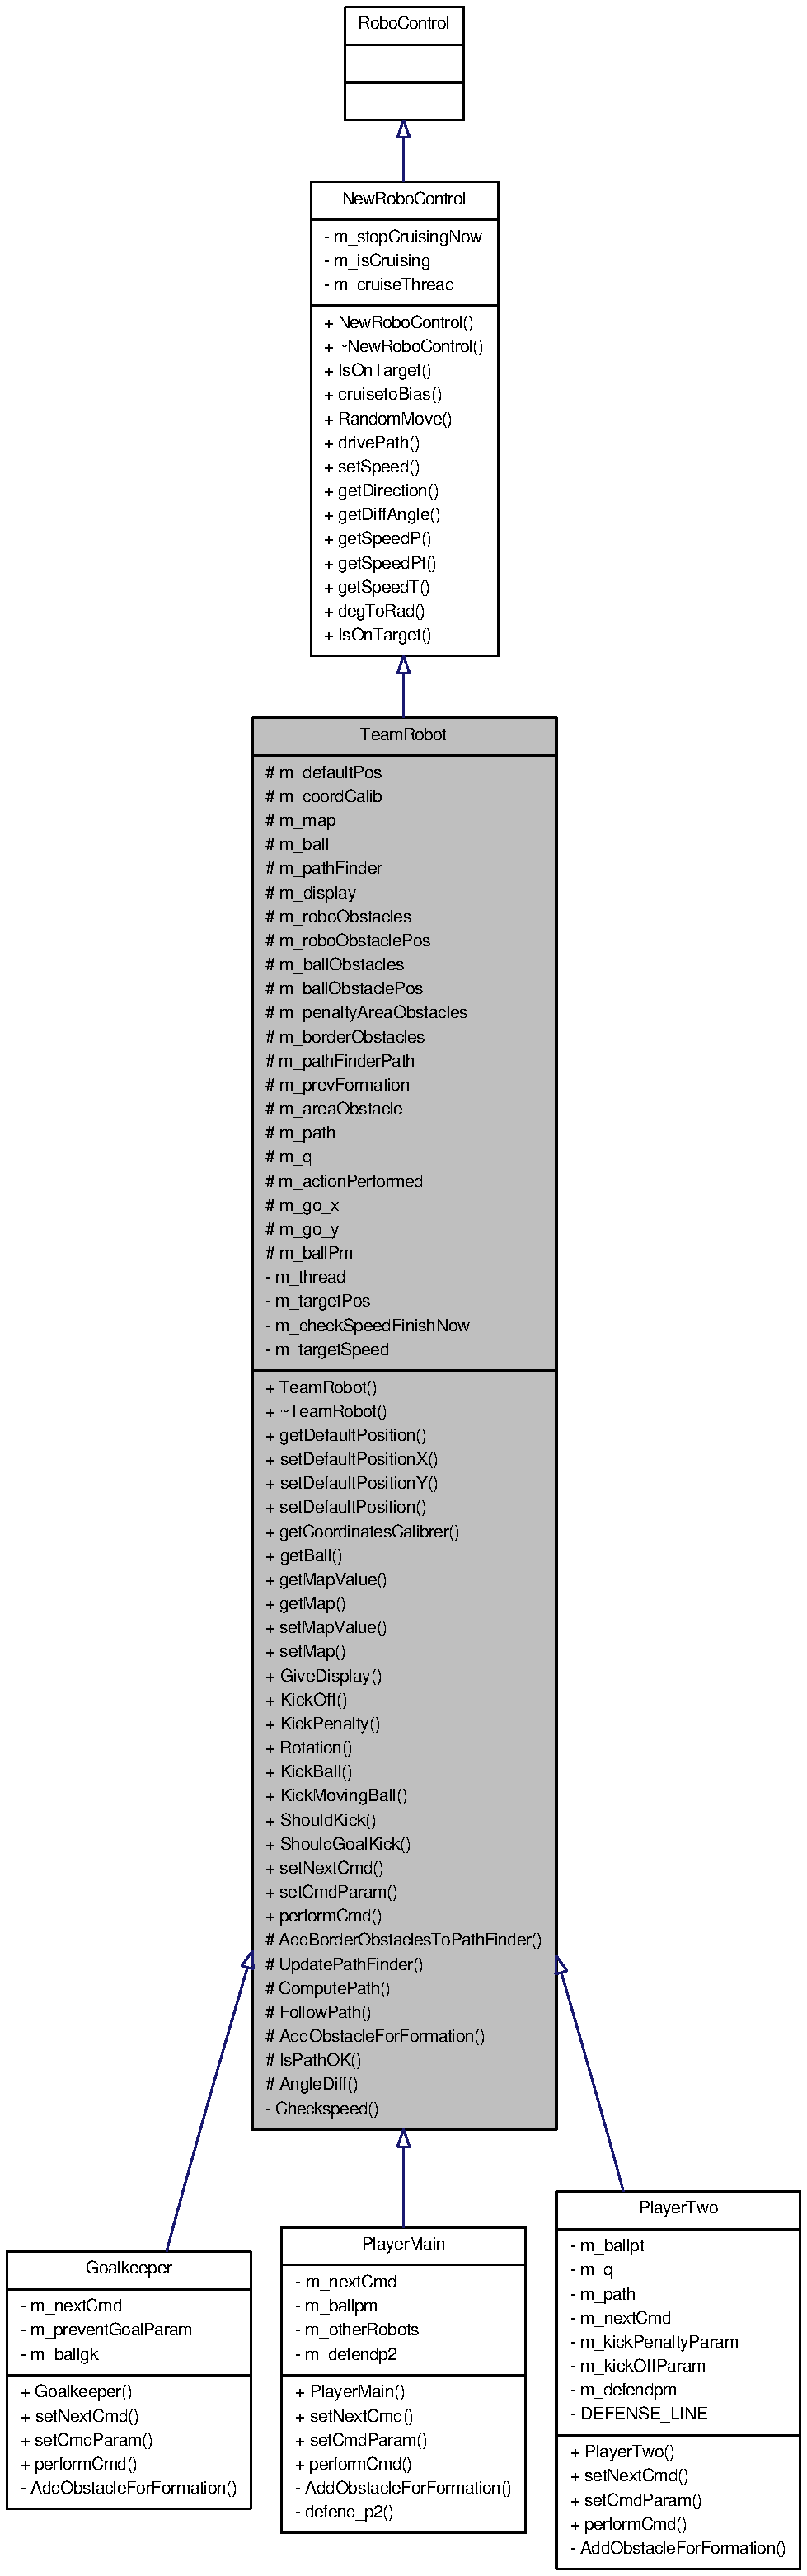
\includegraphics[width=400pt]{classTeamRobot__inherit__graph}
\end{center}
\end{figure}
\subsection*{Public Member Functions}
\begin{DoxyCompactItemize}
\item 
\hyperlink{classTeamRobot_a4b116f58f0a1568a886d03b0c71df20c}{TeamRobot} (RTDBConn \&DBC, const int deviceNr, const \hyperlink{classCoordinatesCalibrer}{CoordinatesCalibrer} $\ast$coordCalib, RawBall $\ast$ball, \hyperlink{classBallMonitor}{BallMonitor} $\ast$ballPm, \hyperlink{classRefereeDisplay}{RefereeDisplay} $\ast$display=NULL)
\item 
virtual \hyperlink{classTeamRobot_a7be9d5161b7524cbbb6ae486ad4a1b42}{$\sim$TeamRobot} ()
\item 
Position \hyperlink{classTeamRobot_acd11ff6d9651a8deddafa5bd9a30865c}{getDefaultPosition} () const 
\begin{DoxyCompactList}\small\item\em using this function the robot get the default position for the current situation \item\end{DoxyCompactList}\item 
void \hyperlink{classTeamRobot_a527cefdb32f2bc0a4fa770207d4dc934}{setDefaultPositionX} (double x)
\begin{DoxyCompactList}\small\item\em this function defines the x of the default position \item\end{DoxyCompactList}\item 
void \hyperlink{classTeamRobot_afeb86cb88b18030049d525d1d6790e6e}{setDefaultPositionY} (double y)
\begin{DoxyCompactList}\small\item\em this function defines the x of the default position \item\end{DoxyCompactList}\item 
void \hyperlink{classTeamRobot_a322f046e260aedff6f2c8edc5730c9ac}{setDefaultPosition} (Position pos)
\begin{DoxyCompactList}\small\item\em this function defines pos of the default position \item\end{DoxyCompactList}\item 
const \hyperlink{classCoordinatesCalibrer}{CoordinatesCalibrer} $\ast$ \hyperlink{classTeamRobot_a3ef7d4538226085ed4d92b8bd2fce67d}{getCoordinatesCalibrer} () const 
\item 
RawBall $\ast$ \hyperlink{classTeamRobot_a86dbc3bbf6fdcebd4ae41a6f68d92a15}{getBall} () const 
\item 
int \hyperlink{classTeamRobot_abc3a5d2d4cac44629a9d8851164b5eda}{getMapValue} (int i, int j) const 
\begin{DoxyCompactList}\small\item\em this function calculate the actual position in the map based on the pathfinder. it unnormalizes from pathfinder to real map \item\end{DoxyCompactList}\item 
const \hyperlink{classMatrix}{Interpreter::Map} \& \hyperlink{classTeamRobot_a8b5fa0d9f42166fc3339ec901fad5a91}{getMap} () const 
\item 
bool \hyperlink{classTeamRobot_a28ee2460e7d465989bb0582782db851e}{setMapValue} (int i, int j, int val)
\item 
void \hyperlink{classTeamRobot_ab8c92b6228aed8eef31d0b1b0fce8690}{setMap} (const \hyperlink{classMatrix}{Interpreter::Map} \&map)
\item 
void \hyperlink{classTeamRobot_a2caa2411b9972fa5caa595f568394ba0}{GiveDisplay} (\hyperlink{classRefereeDisplay}{RefereeDisplay} $\ast$display)
\item 
void \hyperlink{classTeamRobot_a162c8b33d4315a61d8371dc9a923b37b}{KickOff} (const \hyperlink{classNewRoboControl}{NewRoboControl} $\ast$otherRobots\mbox{[}5\mbox{]}, eSide ourSide, bool likePenalty=false)
\item 
void \hyperlink{classTeamRobot_ad5755055df84960c8d1a0a40efe33668}{KickPenalty} (const \hyperlink{classNewRoboControl}{NewRoboControl} $\ast$otherRobots\mbox{[}5\mbox{]})
\item 
bool \hyperlink{classTeamRobot_aa1bb9ac05c067a68118c8646c8d71830}{Rotation} (Position ballPos)
\item 
void \hyperlink{classTeamRobot_a36d006bfeadfcdd37bd1eeb47223bdba}{KickBall} (Position ballPos, bool rotate=true, bool forward=true)
\begin{DoxyCompactList}\small\item\em this function calculate whether the robot should move forwards or backwards to kick the ball. Furthermore, it adjusts the angle of the robot so that the robot can hit the ball precisely. \item\end{DoxyCompactList}\item 
void \hyperlink{classTeamRobot_a98d044ad3907493236b2d399a26cb9ac}{KickMovingBall} (RawBall $\ast$ball)
\item 
bool \hyperlink{classTeamRobot_ac979572f4899940e88f067102ac1ae46}{ShouldKick} (Position ballPos, Position goalPos)
\begin{DoxyCompactList}\small\item\em this function calculate if the robot should kick the ball and kick the ball in the direction of the goal. \item\end{DoxyCompactList}\item 
bool \hyperlink{classTeamRobot_ae7f6fa303c865dad297b662731165883}{ShouldGoalKick} (Position ballPos, eSide ourSide)
\begin{DoxyCompactList}\small\item\em this function let the robot kick the ball if the ball is on our side. in this way the potential dangerous is eliminated \item\end{DoxyCompactList}\item 
virtual void \hyperlink{classTeamRobot_a65f9a2b7464dfac3f4a0336810cf574f}{setNextCmd} (const \hyperlink{structInterpreter_1_1GameData}{Interpreter::GameData} \&info)=0
\item 
virtual void \hyperlink{classTeamRobot_a34c0fd6986c510d4025e5752b3c0e49a}{setCmdParam} (const \hyperlink{classInterpreter}{Interpreter} \&interpreter)=0
\item 
virtual void \hyperlink{classTeamRobot_a9b84df51ca16a7203fdb6498ea6741da}{performCmd} (const \hyperlink{structInterpreter_1_1GameData}{Interpreter::GameData} \&info)=0
\end{DoxyCompactItemize}
\subsection*{Protected Member Functions}
\begin{DoxyCompactItemize}
\item 
void \hyperlink{classTeamRobot_acf4c435c98bc406744a12cd140d6631d}{AddBorderObstaclesToPathFinder} (bool small=false)
\item 
void \hyperlink{classTeamRobot_a1216ffb71821002b6e6845390c990d5f}{UpdatePathFinder} (const \hyperlink{classNewRoboControl}{NewRoboControl} $\ast$obstacles\mbox{[}5\mbox{]}, const \hyperlink{structInterpreter_1_1GameData}{Interpreter::GameData} \&info)
\begin{DoxyCompactList}\small\item\em update the path based on current position of the robots \item\end{DoxyCompactList}\item 
void \hyperlink{classTeamRobot_a9ae431d9eeaa1d16fa28c636499ab553}{ComputePath} (const \hyperlink{classInterpreter}{Interpreter} \&interpreter)
\item 
void \hyperlink{classTeamRobot_a02df00aae0a514badc93a9b2593be85f}{FollowPath} (const \hyperlink{structInterpreter_1_1GameData}{Interpreter::GameData} \&info)
\begin{DoxyCompactList}\small\item\em this function is carried out during the game and it allows the robot to attack and defense properly \item\end{DoxyCompactList}\item 
virtual void \hyperlink{classTeamRobot_a71ec65db46db1ac511fe17b668d4f192}{AddObstacleForFormation} (const \hyperlink{structInterpreter_1_1GameData}{Interpreter::GameData} \&info)=0
\end{DoxyCompactItemize}
\subsection*{Static Protected Member Functions}
\begin{DoxyCompactItemize}
\item 
static bool \hyperlink{classTeamRobot_afb5f9191ca185053af37c1ae1f8dcb17}{IsPathOK} (\hyperlink{classPathFinder_a269aba09b7b3208092f67f2bc02cf63e}{PathFinder::Path} path, \hyperlink{structPathFinder_1_1Point}{PathFinder::Point} \&tgt)
\item 
static double \hyperlink{classTeamRobot_a45d5d631b1e1e28c9c0f4ecbd47fdbde}{AngleDiff} (double angle1, double angle2)
\begin{DoxyCompactList}\small\item\em this function calculate the difference between 2 angles and return the difference value in the range of -\/PI to PI. \item\end{DoxyCompactList}\end{DoxyCompactItemize}
\subsection*{Protected Attributes}
\begin{DoxyCompactItemize}
\item 
Position \hyperlink{classTeamRobot_a5758854ca2d6a084bea074c39e75b5d3}{m\_\-defaultPos}
\item 
const \hyperlink{classCoordinatesCalibrer}{CoordinatesCalibrer} $\ast$ \hyperlink{classTeamRobot_a3bfcb3cdeedcc11eaed1b5bce532560f}{m\_\-coordCalib}
\item 
\hyperlink{classMatrix}{Interpreter::Map} \hyperlink{classTeamRobot_acf38fcc5b3c4ab4815fb151e39d5889c}{m\_\-map}
\item 
RawBall $\ast$ \hyperlink{classTeamRobot_ac6544ce7a73fe05e3c9a69cc50b58bbe}{m\_\-ball}
\item 
\hyperlink{classPathFinder}{PathFinder} \hyperlink{classTeamRobot_ac5845718f0d540e3f17f39d62d6f11c7}{m\_\-pathFinder}
\item 
\hyperlink{classRefereeDisplay}{RefereeDisplay} $\ast$ \hyperlink{classTeamRobot_aecbb2869966fba9b3de3cbc530c7bc36}{m\_\-display}
\item 
const \hyperlink{structPathFinder_1_1ConvexPolygon}{PathFinder::ConvexPolygon} $\ast$ \hyperlink{classTeamRobot_a9dc410e800f251d62dbde6b3791b2009}{m\_\-roboObstacles} \mbox{[}5\mbox{]}
\item 
Position \hyperlink{classTeamRobot_a5337cff2b594fd63b2445c1d49374d7e}{m\_\-roboObstaclePos} \mbox{[}5\mbox{]}
\item 
const \hyperlink{structPathFinder_1_1ConvexPolygon}{PathFinder::ConvexPolygon} $\ast$ \hyperlink{classTeamRobot_a06fd18a201a66f021e0c72dfd845e26b}{m\_\-ballObstacles} \mbox{[}3\mbox{]}
\item 
Position \hyperlink{classTeamRobot_aba2294985cc9a1dc404271e29166da82}{m\_\-ballObstaclePos}
\item 
const \hyperlink{structPathFinder_1_1ConvexPolygon}{PathFinder::ConvexPolygon} $\ast$ \hyperlink{classTeamRobot_a155fbee5f74459799332801b09c99616}{m\_\-penaltyAreaObstacles} \mbox{[}2\mbox{]}
\item 
const \hyperlink{structPathFinder_1_1ConvexPolygon}{PathFinder::ConvexPolygon} $\ast$ \hyperlink{classTeamRobot_a0292337f910ac2bbb300affb87891ba7}{m\_\-borderObstacles} \mbox{[}4\mbox{]}
\item 
\hyperlink{classPathFinder_a269aba09b7b3208092f67f2bc02cf63e}{PathFinder::Path} \hyperlink{classTeamRobot_aca22e17bd02f1ce84786ed2194764afa}{m\_\-pathFinderPath}
\item 
\hyperlink{classInterpreter_a0fb49436c8c14ca79e13f1cd78119088}{Interpreter::Strategy} \hyperlink{classTeamRobot_ab32d14c3de4fd5a6ff6db39eb04f52f2}{m\_\-prevFormation}
\item 
const \hyperlink{structPathFinder_1_1ConvexPolygon}{PathFinder::ConvexPolygon} $\ast$ \hyperlink{classTeamRobot_af06d7a399ac2a3c24c27a7af1c6e38e5}{m\_\-areaObstacle}
\item 
string \hyperlink{classTeamRobot_af170b8d2e1b76b12f8cc83f6ec908e40}{m\_\-path}
\item 
queue$<$ int $>$ \hyperlink{classTeamRobot_a982ed6b6964c5e8b94519ef91b52c468}{m\_\-q}
\item 
bool \hyperlink{classTeamRobot_ab98a148247f0c8bbadac3cfc8fa268c8}{m\_\-actionPerformed}
\item 
int \hyperlink{classTeamRobot_ae4bafa3b5f0df155b1a45f95f6671316}{m\_\-go\_\-x}
\item 
int \hyperlink{classTeamRobot_ad0b6cee88278087238bf6fcecb419808}{m\_\-go\_\-y}
\item 
\hyperlink{classBallMonitor}{BallMonitor} $\ast$ \hyperlink{classTeamRobot_a84b5181a2fadaf7653d32f04fa04d657}{m\_\-ballPm}
\end{DoxyCompactItemize}
\subsection*{Static Private Member Functions}
\begin{DoxyCompactItemize}
\item 
static void $\ast$ \hyperlink{classTeamRobot_ac52f7f240fde40db09116e8639a53c21}{Checkspeed} (void $\ast$data)
\begin{DoxyCompactList}\small\item\em moves the robot to a random position if it stucks somewhere. \item\end{DoxyCompactList}\end{DoxyCompactItemize}
\subsection*{Private Attributes}
\begin{DoxyCompactItemize}
\item 
pthread\_\-t \hyperlink{classTeamRobot_a3e9052964ba03b6dce4a34d1e45dbb1f}{m\_\-thread}
\item 
Position \hyperlink{classTeamRobot_ab7446260b71870667a83b8c53e1274be}{m\_\-targetPos}
\item 
bool \hyperlink{classTeamRobot_ac4229cdeb227ab578cfe38023af2db59}{m\_\-checkSpeedFinishNow}
\item 
double \hyperlink{classTeamRobot_aaea621727542377ed5d5e1a316c5293c}{m\_\-targetSpeed}
\end{DoxyCompactItemize}


\subsection{Detailed Description}
Abstract child class of \hyperlink{classNewRoboControl}{NewRoboControl} describing a robot from our team. This class implements more high-\/level dring functions such as path computation / driving or kick functions. This class must be inherited to be constructed, and the child classes must implement the four virtual methods \hyperlink{classTeamRobot_a65f9a2b7464dfac3f4a0336810cf574f}{TeamRobot::setNextCmd()}, \hyperlink{classTeamRobot_a34c0fd6986c510d4025e5752b3c0e49a}{TeamRobot::setCmdParam()}, \hyperlink{classTeamRobot_a9b84df51ca16a7203fdb6498ea6741da}{TeamRobot::performCmd()} and \hyperlink{classTeamRobot_a71ec65db46db1ac511fe17b668d4f192}{TeamRobot::AddObstacleForFormation()}. 

\subsection{Constructor \& Destructor Documentation}
\hypertarget{classTeamRobot_a4b116f58f0a1568a886d03b0c71df20c}{
\index{TeamRobot@{TeamRobot}!TeamRobot@{TeamRobot}}
\index{TeamRobot@{TeamRobot}!TeamRobot@{TeamRobot}}
\subsubsection[{TeamRobot}]{\setlength{\rightskip}{0pt plus 5cm}TeamRobot::TeamRobot (RTDBConn \& {\em DBC}, \/  const int {\em deviceNr}, \/  const {\bf CoordinatesCalibrer} $\ast$ {\em coordCalib}, \/  RawBall $\ast$ {\em ball}, \/  {\bf BallMonitor} $\ast$ {\em ballPm}, \/  {\bf RefereeDisplay} $\ast$ {\em display} = {\ttfamily NULL})}}
\label{classTeamRobot_a4b116f58f0a1568a886d03b0c71df20c}

\begin{DoxyParams}{Parameters}
\item[{\em DBC}]\item[{\em deviceNr}]\item[{\em coordCalib}]\item[{\em ball}]\item[{\em ballPm}]\item[{\em display}]\end{DoxyParams}
\hypertarget{classTeamRobot_a7be9d5161b7524cbbb6ae486ad4a1b42}{
\index{TeamRobot@{TeamRobot}!$\sim$TeamRobot@{$\sim$TeamRobot}}
\index{$\sim$TeamRobot@{$\sim$TeamRobot}!TeamRobot@{TeamRobot}}
\subsubsection[{$\sim$TeamRobot}]{\setlength{\rightskip}{0pt plus 5cm}TeamRobot::$\sim$TeamRobot ()\hspace{0.3cm}{\ttfamily  \mbox{[}virtual\mbox{]}}}}
\label{classTeamRobot_a7be9d5161b7524cbbb6ae486ad4a1b42}


\subsection{Member Function Documentation}
\hypertarget{classTeamRobot_acf4c435c98bc406744a12cd140d6631d}{
\index{TeamRobot@{TeamRobot}!AddBorderObstaclesToPathFinder@{AddBorderObstaclesToPathFinder}}
\index{AddBorderObstaclesToPathFinder@{AddBorderObstaclesToPathFinder}!TeamRobot@{TeamRobot}}
\subsubsection[{AddBorderObstaclesToPathFinder}]{\setlength{\rightskip}{0pt plus 5cm}void TeamRobot::AddBorderObstaclesToPathFinder (bool {\em small} = {\ttfamily false})\hspace{0.3cm}{\ttfamily  \mbox{[}protected\mbox{]}}}}
\label{classTeamRobot_acf4c435c98bc406744a12cd140d6631d}

\begin{DoxyParams}{Parameters}
\item[{\em small}]\end{DoxyParams}
\hypertarget{classTeamRobot_a71ec65db46db1ac511fe17b668d4f192}{
\index{TeamRobot@{TeamRobot}!AddObstacleForFormation@{AddObstacleForFormation}}
\index{AddObstacleForFormation@{AddObstacleForFormation}!TeamRobot@{TeamRobot}}
\subsubsection[{AddObstacleForFormation}]{\setlength{\rightskip}{0pt plus 5cm}virtual void TeamRobot::AddObstacleForFormation (const {\bf Interpreter::GameData} \& {\em info})\hspace{0.3cm}{\ttfamily  \mbox{[}protected, pure virtual\mbox{]}}}}
\label{classTeamRobot_a71ec65db46db1ac511fe17b668d4f192}


Implemented in \hyperlink{classGoalkeeper_a5287a2e74795bbec8f0ead767655da5d}{Goalkeeper}, \hyperlink{classPlayerMain_a978b3ce16f5d8e5d1cb9ef70f387227e}{PlayerMain}, and \hyperlink{classPlayerTwo_a9e3341541658f54a2dfb0491a774b4d4}{PlayerTwo}.

\hypertarget{classTeamRobot_a45d5d631b1e1e28c9c0f4ecbd47fdbde}{
\index{TeamRobot@{TeamRobot}!AngleDiff@{AngleDiff}}
\index{AngleDiff@{AngleDiff}!TeamRobot@{TeamRobot}}
\subsubsection[{AngleDiff}]{\setlength{\rightskip}{0pt plus 5cm}double TeamRobot::AngleDiff (double {\em angle1}, \/  double {\em angle2})\hspace{0.3cm}{\ttfamily  \mbox{[}static, protected\mbox{]}}}}
\label{classTeamRobot_a45d5d631b1e1e28c9c0f4ecbd47fdbde}


this function calculate the difference between 2 angles and return the difference value in the range of -\/PI to PI. 


\begin{DoxyParams}{Parameters}
\item[{\em angle1}]\item[{\em angle2}]\end{DoxyParams}
\begin{DoxyReturn}{Returns}
double the difference between angle1 and angle2 
\end{DoxyReturn}
\hypertarget{classTeamRobot_ac52f7f240fde40db09116e8639a53c21}{
\index{TeamRobot@{TeamRobot}!Checkspeed@{Checkspeed}}
\index{Checkspeed@{Checkspeed}!TeamRobot@{TeamRobot}}
\subsubsection[{Checkspeed}]{\setlength{\rightskip}{0pt plus 5cm}void $\ast$ TeamRobot::Checkspeed (void $\ast$ {\em data})\hspace{0.3cm}{\ttfamily  \mbox{[}static, private\mbox{]}}}}
\label{classTeamRobot_ac52f7f240fde40db09116e8639a53c21}


moves the robot to a random position if it stucks somewhere. 


\begin{DoxyParams}{Parameters}
\item[{\em data}]is the robot \end{DoxyParams}
\hypertarget{classTeamRobot_a9ae431d9eeaa1d16fa28c636499ab553}{
\index{TeamRobot@{TeamRobot}!ComputePath@{ComputePath}}
\index{ComputePath@{ComputePath}!TeamRobot@{TeamRobot}}
\subsubsection[{ComputePath}]{\setlength{\rightskip}{0pt plus 5cm}void TeamRobot::ComputePath (const {\bf Interpreter} \& {\em interpreter})\hspace{0.3cm}{\ttfamily  \mbox{[}protected\mbox{]}}}}
\label{classTeamRobot_a9ae431d9eeaa1d16fa28c636499ab553}

\begin{DoxyParams}{Parameters}
\item[{\em interpreter}]\end{DoxyParams}
\hypertarget{classTeamRobot_a02df00aae0a514badc93a9b2593be85f}{
\index{TeamRobot@{TeamRobot}!FollowPath@{FollowPath}}
\index{FollowPath@{FollowPath}!TeamRobot@{TeamRobot}}
\subsubsection[{FollowPath}]{\setlength{\rightskip}{0pt plus 5cm}void TeamRobot::FollowPath (const {\bf Interpreter::GameData} \& {\em info})\hspace{0.3cm}{\ttfamily  \mbox{[}protected\mbox{]}}}}
\label{classTeamRobot_a02df00aae0a514badc93a9b2593be85f}


this function is carried out during the game and it allows the robot to attack and defense properly 


\begin{DoxyParams}{Parameters}
\item[{\em info}]is current playmode of referee \end{DoxyParams}
\hypertarget{classTeamRobot_a86dbc3bbf6fdcebd4ae41a6f68d92a15}{
\index{TeamRobot@{TeamRobot}!getBall@{getBall}}
\index{getBall@{getBall}!TeamRobot@{TeamRobot}}
\subsubsection[{getBall}]{\setlength{\rightskip}{0pt plus 5cm}RawBall $\ast$ TeamRobot::getBall () const}}
\label{classTeamRobot_a86dbc3bbf6fdcebd4ae41a6f68d92a15}
\begin{DoxyReturn}{Returns}
RawBall $\ast$ 
\end{DoxyReturn}
\hypertarget{classTeamRobot_a3ef7d4538226085ed4d92b8bd2fce67d}{
\index{TeamRobot@{TeamRobot}!getCoordinatesCalibrer@{getCoordinatesCalibrer}}
\index{getCoordinatesCalibrer@{getCoordinatesCalibrer}!TeamRobot@{TeamRobot}}
\subsubsection[{getCoordinatesCalibrer}]{\setlength{\rightskip}{0pt plus 5cm}const {\bf CoordinatesCalibrer} $\ast$ TeamRobot::getCoordinatesCalibrer () const}}
\label{classTeamRobot_a3ef7d4538226085ed4d92b8bd2fce67d}
\begin{DoxyReturn}{Returns}
const \hyperlink{classCoordinatesCalibrer}{CoordinatesCalibrer} $\ast$ 
\end{DoxyReturn}
\hypertarget{classTeamRobot_acd11ff6d9651a8deddafa5bd9a30865c}{
\index{TeamRobot@{TeamRobot}!getDefaultPosition@{getDefaultPosition}}
\index{getDefaultPosition@{getDefaultPosition}!TeamRobot@{TeamRobot}}
\subsubsection[{getDefaultPosition}]{\setlength{\rightskip}{0pt plus 5cm}Position TeamRobot::getDefaultPosition () const}}
\label{classTeamRobot_acd11ff6d9651a8deddafa5bd9a30865c}


using this function the robot get the default position for the current situation 

\begin{DoxyReturn}{Returns}
Position is the default position. 
\end{DoxyReturn}
\hypertarget{classTeamRobot_a8b5fa0d9f42166fc3339ec901fad5a91}{
\index{TeamRobot@{TeamRobot}!getMap@{getMap}}
\index{getMap@{getMap}!TeamRobot@{TeamRobot}}
\subsubsection[{getMap}]{\setlength{\rightskip}{0pt plus 5cm}const {\bf Interpreter::Map} \& TeamRobot::getMap () const}}
\label{classTeamRobot_a8b5fa0d9f42166fc3339ec901fad5a91}
\begin{DoxyReturn}{Returns}
const \hyperlink{classInterpreter_a4c080f069f557cf92dfe803117a6ea53}{Interpreter::Map} \& 
\end{DoxyReturn}
\hypertarget{classTeamRobot_abc3a5d2d4cac44629a9d8851164b5eda}{
\index{TeamRobot@{TeamRobot}!getMapValue@{getMapValue}}
\index{getMapValue@{getMapValue}!TeamRobot@{TeamRobot}}
\subsubsection[{getMapValue}]{\setlength{\rightskip}{0pt plus 5cm}int TeamRobot::getMapValue (int {\em i}, \/  int {\em j}) const}}
\label{classTeamRobot_abc3a5d2d4cac44629a9d8851164b5eda}


this function calculate the actual position in the map based on the pathfinder. it unnormalizes from pathfinder to real map 


\begin{DoxyParams}{Parameters}
\item[{\em i}]is value on x axis in pathfinder \item[{\em j}]is value on y axis in pathfinder \end{DoxyParams}
\begin{DoxyReturn}{Returns}
int 
\end{DoxyReturn}
\hypertarget{classTeamRobot_a2caa2411b9972fa5caa595f568394ba0}{
\index{TeamRobot@{TeamRobot}!GiveDisplay@{GiveDisplay}}
\index{GiveDisplay@{GiveDisplay}!TeamRobot@{TeamRobot}}
\subsubsection[{GiveDisplay}]{\setlength{\rightskip}{0pt plus 5cm}void TeamRobot::GiveDisplay ({\bf RefereeDisplay} $\ast$ {\em display})}}
\label{classTeamRobot_a2caa2411b9972fa5caa595f568394ba0}

\begin{DoxyParams}{Parameters}
\item[{\em display}]\end{DoxyParams}
\hypertarget{classTeamRobot_afb5f9191ca185053af37c1ae1f8dcb17}{
\index{TeamRobot@{TeamRobot}!IsPathOK@{IsPathOK}}
\index{IsPathOK@{IsPathOK}!TeamRobot@{TeamRobot}}
\subsubsection[{IsPathOK}]{\setlength{\rightskip}{0pt plus 5cm}bool TeamRobot::IsPathOK ({\bf PathFinder::Path} {\em path}, \/  {\bf PathFinder::Point} \& {\em tgt})\hspace{0.3cm}{\ttfamily  \mbox{[}static, protected\mbox{]}}}}
\label{classTeamRobot_afb5f9191ca185053af37c1ae1f8dcb17}

\begin{DoxyParams}{Parameters}
\item[{\em path}]\item[{\em tgt}]\end{DoxyParams}
\begin{DoxyReturn}{Returns}
bool 
\end{DoxyReturn}
\hypertarget{classTeamRobot_a36d006bfeadfcdd37bd1eeb47223bdba}{
\index{TeamRobot@{TeamRobot}!KickBall@{KickBall}}
\index{KickBall@{KickBall}!TeamRobot@{TeamRobot}}
\subsubsection[{KickBall}]{\setlength{\rightskip}{0pt plus 5cm}void TeamRobot::KickBall (Position {\em ballPos}, \/  bool {\em rotate} = {\ttfamily true}, \/  bool {\em forward} = {\ttfamily true})}}
\label{classTeamRobot_a36d006bfeadfcdd37bd1eeb47223bdba}


this function calculate whether the robot should move forwards or backwards to kick the ball. Furthermore, it adjusts the angle of the robot so that the robot can hit the ball precisely. 


\begin{DoxyParams}{Parameters}
\item[{\em ballPos}]is the position of the ball \item[{\em rotate}]True if the robot should rotate towards the ball before kicking \item[{\em forward}]True if the kick must be done forward, False if it must be done backwards, ignored if rotate is True. \end{DoxyParams}
\hypertarget{classTeamRobot_a98d044ad3907493236b2d399a26cb9ac}{
\index{TeamRobot@{TeamRobot}!KickMovingBall@{KickMovingBall}}
\index{KickMovingBall@{KickMovingBall}!TeamRobot@{TeamRobot}}
\subsubsection[{KickMovingBall}]{\setlength{\rightskip}{0pt plus 5cm}void TeamRobot::KickMovingBall (RawBall $\ast$ {\em ball})}}
\label{classTeamRobot_a98d044ad3907493236b2d399a26cb9ac}

\begin{DoxyParams}{Parameters}
\item[{\em ball}]\end{DoxyParams}
\hypertarget{classTeamRobot_a162c8b33d4315a61d8371dc9a923b37b}{
\index{TeamRobot@{TeamRobot}!KickOff@{KickOff}}
\index{KickOff@{KickOff}!TeamRobot@{TeamRobot}}
\subsubsection[{KickOff}]{\setlength{\rightskip}{0pt plus 5cm}void TeamRobot::KickOff (const {\bf NewRoboControl} $\ast$ {\em otherRobots}\mbox{[}5\mbox{]}, \/  eSide {\em ourSide}, \/  bool {\em likePenalty} = {\ttfamily false})}}
\label{classTeamRobot_a162c8b33d4315a61d8371dc9a923b37b}

\begin{DoxyParams}{Parameters}
\item[{\em otherRobots\mbox{[}$\,$\mbox{]}}]\item[{\em ourSide}]\item[{\em likePenalty}]\end{DoxyParams}
\hypertarget{classTeamRobot_ad5755055df84960c8d1a0a40efe33668}{
\index{TeamRobot@{TeamRobot}!KickPenalty@{KickPenalty}}
\index{KickPenalty@{KickPenalty}!TeamRobot@{TeamRobot}}
\subsubsection[{KickPenalty}]{\setlength{\rightskip}{0pt plus 5cm}void TeamRobot::KickPenalty (const {\bf NewRoboControl} $\ast$ {\em otherRobots}\mbox{[}5\mbox{]})}}
\label{classTeamRobot_ad5755055df84960c8d1a0a40efe33668}

\begin{DoxyParams}{Parameters}
\item[{\em otherRobots\mbox{[}$\,$\mbox{]}}]\end{DoxyParams}
\hypertarget{classTeamRobot_a9b84df51ca16a7203fdb6498ea6741da}{
\index{TeamRobot@{TeamRobot}!performCmd@{performCmd}}
\index{performCmd@{performCmd}!TeamRobot@{TeamRobot}}
\subsubsection[{performCmd}]{\setlength{\rightskip}{0pt plus 5cm}virtual void TeamRobot::performCmd (const {\bf Interpreter::GameData} \& {\em info})\hspace{0.3cm}{\ttfamily  \mbox{[}pure virtual\mbox{]}}}}
\label{classTeamRobot_a9b84df51ca16a7203fdb6498ea6741da}


Implemented in \hyperlink{classGoalkeeper_ab850d0d2278730bebc5479f1a339a925}{Goalkeeper}, \hyperlink{classPlayerMain_af12a95c226ce973056681a138b55fb6c}{PlayerMain}, and \hyperlink{classPlayerTwo_a56d794b718c60092a324f312b8333eb9}{PlayerTwo}.

\hypertarget{classTeamRobot_aa1bb9ac05c067a68118c8646c8d71830}{
\index{TeamRobot@{TeamRobot}!Rotation@{Rotation}}
\index{Rotation@{Rotation}!TeamRobot@{TeamRobot}}
\subsubsection[{Rotation}]{\setlength{\rightskip}{0pt plus 5cm}bool TeamRobot::Rotation (Position {\em ballPos})}}
\label{classTeamRobot_aa1bb9ac05c067a68118c8646c8d71830}
\hypertarget{classTeamRobot_a34c0fd6986c510d4025e5752b3c0e49a}{
\index{TeamRobot@{TeamRobot}!setCmdParam@{setCmdParam}}
\index{setCmdParam@{setCmdParam}!TeamRobot@{TeamRobot}}
\subsubsection[{setCmdParam}]{\setlength{\rightskip}{0pt plus 5cm}virtual void TeamRobot::setCmdParam (const {\bf Interpreter} \& {\em interpreter})\hspace{0.3cm}{\ttfamily  \mbox{[}pure virtual\mbox{]}}}}
\label{classTeamRobot_a34c0fd6986c510d4025e5752b3c0e49a}


Implemented in \hyperlink{classGoalkeeper_acfa6fbad0f6b1627fd59cc7cce6ff321}{Goalkeeper}, \hyperlink{classPlayerMain_a5c4af159392663660f91809052422945}{PlayerMain}, and \hyperlink{classPlayerTwo_aa0294cf24297f66ffd92f1a250794340}{PlayerTwo}.

\hypertarget{classTeamRobot_a322f046e260aedff6f2c8edc5730c9ac}{
\index{TeamRobot@{TeamRobot}!setDefaultPosition@{setDefaultPosition}}
\index{setDefaultPosition@{setDefaultPosition}!TeamRobot@{TeamRobot}}
\subsubsection[{setDefaultPosition}]{\setlength{\rightskip}{0pt plus 5cm}void TeamRobot::setDefaultPosition (Position {\em pos})}}
\label{classTeamRobot_a322f046e260aedff6f2c8edc5730c9ac}


this function defines pos of the default position 


\begin{DoxyParams}{Parameters}
\item[{\em pos}]is the value of current default position \end{DoxyParams}
\hypertarget{classTeamRobot_a527cefdb32f2bc0a4fa770207d4dc934}{
\index{TeamRobot@{TeamRobot}!setDefaultPositionX@{setDefaultPositionX}}
\index{setDefaultPositionX@{setDefaultPositionX}!TeamRobot@{TeamRobot}}
\subsubsection[{setDefaultPositionX}]{\setlength{\rightskip}{0pt plus 5cm}void TeamRobot::setDefaultPositionX (double {\em x})}}
\label{classTeamRobot_a527cefdb32f2bc0a4fa770207d4dc934}


this function defines the x of the default position 


\begin{DoxyParams}{Parameters}
\item[{\em x}]is the X value of current default position \end{DoxyParams}
\hypertarget{classTeamRobot_afeb86cb88b18030049d525d1d6790e6e}{
\index{TeamRobot@{TeamRobot}!setDefaultPositionY@{setDefaultPositionY}}
\index{setDefaultPositionY@{setDefaultPositionY}!TeamRobot@{TeamRobot}}
\subsubsection[{setDefaultPositionY}]{\setlength{\rightskip}{0pt plus 5cm}void TeamRobot::setDefaultPositionY (double {\em y})}}
\label{classTeamRobot_afeb86cb88b18030049d525d1d6790e6e}


this function defines the x of the default position 


\begin{DoxyParams}{Parameters}
\item[{\em y}]is the Y value of current default position \end{DoxyParams}
\hypertarget{classTeamRobot_ab8c92b6228aed8eef31d0b1b0fce8690}{
\index{TeamRobot@{TeamRobot}!setMap@{setMap}}
\index{setMap@{setMap}!TeamRobot@{TeamRobot}}
\subsubsection[{setMap}]{\setlength{\rightskip}{0pt plus 5cm}void TeamRobot::setMap (const {\bf Interpreter::Map} \& {\em map})}}
\label{classTeamRobot_ab8c92b6228aed8eef31d0b1b0fce8690}

\begin{DoxyParams}{Parameters}
\item[{\em map}]\end{DoxyParams}
\hypertarget{classTeamRobot_a28ee2460e7d465989bb0582782db851e}{
\index{TeamRobot@{TeamRobot}!setMapValue@{setMapValue}}
\index{setMapValue@{setMapValue}!TeamRobot@{TeamRobot}}
\subsubsection[{setMapValue}]{\setlength{\rightskip}{0pt plus 5cm}bool TeamRobot::setMapValue (int {\em i}, \/  int {\em j}, \/  int {\em val})}}
\label{classTeamRobot_a28ee2460e7d465989bb0582782db851e}

\begin{DoxyParams}{Parameters}
\item[{\em i}]\item[{\em j}]\item[{\em val}]\end{DoxyParams}
\begin{DoxyReturn}{Returns}
bool 
\end{DoxyReturn}
\hypertarget{classTeamRobot_a65f9a2b7464dfac3f4a0336810cf574f}{
\index{TeamRobot@{TeamRobot}!setNextCmd@{setNextCmd}}
\index{setNextCmd@{setNextCmd}!TeamRobot@{TeamRobot}}
\subsubsection[{setNextCmd}]{\setlength{\rightskip}{0pt plus 5cm}virtual void TeamRobot::setNextCmd (const {\bf Interpreter::GameData} \& {\em info})\hspace{0.3cm}{\ttfamily  \mbox{[}pure virtual\mbox{]}}}}
\label{classTeamRobot_a65f9a2b7464dfac3f4a0336810cf574f}


Implemented in \hyperlink{classGoalkeeper_abc394351f7c0d552c6e96da422c772ec}{Goalkeeper}, \hyperlink{classPlayerMain_a8f0320189df15529662c7f16d2f74084}{PlayerMain}, and \hyperlink{classPlayerTwo_a7ac9a9a4f1dedee2006e6a0c79f37c0c}{PlayerTwo}.

\hypertarget{classTeamRobot_ae7f6fa303c865dad297b662731165883}{
\index{TeamRobot@{TeamRobot}!ShouldGoalKick@{ShouldGoalKick}}
\index{ShouldGoalKick@{ShouldGoalKick}!TeamRobot@{TeamRobot}}
\subsubsection[{ShouldGoalKick}]{\setlength{\rightskip}{0pt plus 5cm}bool TeamRobot::ShouldGoalKick (Position {\em ballPos}, \/  eSide {\em ourSide})}}
\label{classTeamRobot_ae7f6fa303c865dad297b662731165883}


this function let the robot kick the ball if the ball is on our side. in this way the potential dangerous is eliminated 


\begin{DoxyParams}{Parameters}
\item[{\em ballPos}]is the position of the ball \item[{\em ourSide}]the side we are right now. \end{DoxyParams}
\begin{DoxyReturn}{Returns}
bool return false if ball is still far away from the robot 
\end{DoxyReturn}
\hypertarget{classTeamRobot_ac979572f4899940e88f067102ac1ae46}{
\index{TeamRobot@{TeamRobot}!ShouldKick@{ShouldKick}}
\index{ShouldKick@{ShouldKick}!TeamRobot@{TeamRobot}}
\subsubsection[{ShouldKick}]{\setlength{\rightskip}{0pt plus 5cm}bool TeamRobot::ShouldKick (Position {\em ballPos}, \/  Position {\em goalPos})}}
\label{classTeamRobot_ac979572f4899940e88f067102ac1ae46}


this function calculate if the robot should kick the ball and kick the ball in the direction of the goal. 


\begin{DoxyParams}{Parameters}
\item[{\em ballPos}]is the position of the ball \item[{\em goalPos}]is the position of the goal \end{DoxyParams}
\begin{DoxyReturn}{Returns}
bool is false if the ball is still far away from the robot 
\end{DoxyReturn}
\hypertarget{classTeamRobot_a1216ffb71821002b6e6845390c990d5f}{
\index{TeamRobot@{TeamRobot}!UpdatePathFinder@{UpdatePathFinder}}
\index{UpdatePathFinder@{UpdatePathFinder}!TeamRobot@{TeamRobot}}
\subsubsection[{UpdatePathFinder}]{\setlength{\rightskip}{0pt plus 5cm}void TeamRobot::UpdatePathFinder (const {\bf NewRoboControl} $\ast$ {\em obstacles}\mbox{[}5\mbox{]}, \/  const {\bf Interpreter::GameData} \& {\em info})\hspace{0.3cm}{\ttfamily  \mbox{[}protected\mbox{]}}}}
\label{classTeamRobot_a1216ffb71821002b6e6845390c990d5f}


update the path based on current position of the robots 


\begin{DoxyParams}{Parameters}
\item[{\em obstacles\mbox{[}$\,$\mbox{]}}]are all other robots \item[{\em info}]is current playmode of referee \end{DoxyParams}


\subsection{Member Data Documentation}
\hypertarget{classTeamRobot_ab98a148247f0c8bbadac3cfc8fa268c8}{
\index{TeamRobot@{TeamRobot}!m\_\-actionPerformed@{m\_\-actionPerformed}}
\index{m\_\-actionPerformed@{m\_\-actionPerformed}!TeamRobot@{TeamRobot}}
\subsubsection[{m\_\-actionPerformed}]{\setlength{\rightskip}{0pt plus 5cm}bool {\bf TeamRobot::m\_\-actionPerformed}\hspace{0.3cm}{\ttfamily  \mbox{[}protected\mbox{]}}}}
\label{classTeamRobot_ab98a148247f0c8bbadac3cfc8fa268c8}
TODO \hypertarget{classTeamRobot_af06d7a399ac2a3c24c27a7af1c6e38e5}{
\index{TeamRobot@{TeamRobot}!m\_\-areaObstacle@{m\_\-areaObstacle}}
\index{m\_\-areaObstacle@{m\_\-areaObstacle}!TeamRobot@{TeamRobot}}
\subsubsection[{m\_\-areaObstacle}]{\setlength{\rightskip}{0pt plus 5cm}const {\bf PathFinder::ConvexPolygon}$\ast$ {\bf TeamRobot::m\_\-areaObstacle}\hspace{0.3cm}{\ttfamily  \mbox{[}protected\mbox{]}}}}
\label{classTeamRobot_af06d7a399ac2a3c24c27a7af1c6e38e5}
TODO \hypertarget{classTeamRobot_ac6544ce7a73fe05e3c9a69cc50b58bbe}{
\index{TeamRobot@{TeamRobot}!m\_\-ball@{m\_\-ball}}
\index{m\_\-ball@{m\_\-ball}!TeamRobot@{TeamRobot}}
\subsubsection[{m\_\-ball}]{\setlength{\rightskip}{0pt plus 5cm}RawBall$\ast$ {\bf TeamRobot::m\_\-ball}\hspace{0.3cm}{\ttfamily  \mbox{[}protected\mbox{]}}}}
\label{classTeamRobot_ac6544ce7a73fe05e3c9a69cc50b58bbe}
TODO \hypertarget{classTeamRobot_aba2294985cc9a1dc404271e29166da82}{
\index{TeamRobot@{TeamRobot}!m\_\-ballObstaclePos@{m\_\-ballObstaclePos}}
\index{m\_\-ballObstaclePos@{m\_\-ballObstaclePos}!TeamRobot@{TeamRobot}}
\subsubsection[{m\_\-ballObstaclePos}]{\setlength{\rightskip}{0pt plus 5cm}Position {\bf TeamRobot::m\_\-ballObstaclePos}\hspace{0.3cm}{\ttfamily  \mbox{[}protected\mbox{]}}}}
\label{classTeamRobot_aba2294985cc9a1dc404271e29166da82}
TODO \hypertarget{classTeamRobot_a06fd18a201a66f021e0c72dfd845e26b}{
\index{TeamRobot@{TeamRobot}!m\_\-ballObstacles@{m\_\-ballObstacles}}
\index{m\_\-ballObstacles@{m\_\-ballObstacles}!TeamRobot@{TeamRobot}}
\subsubsection[{m\_\-ballObstacles}]{\setlength{\rightskip}{0pt plus 5cm}const {\bf PathFinder::ConvexPolygon}$\ast$ {\bf TeamRobot::m\_\-ballObstacles}\mbox{[}3\mbox{]}\hspace{0.3cm}{\ttfamily  \mbox{[}protected\mbox{]}}}}
\label{classTeamRobot_a06fd18a201a66f021e0c72dfd845e26b}
TODO \hypertarget{classTeamRobot_a84b5181a2fadaf7653d32f04fa04d657}{
\index{TeamRobot@{TeamRobot}!m\_\-ballPm@{m\_\-ballPm}}
\index{m\_\-ballPm@{m\_\-ballPm}!TeamRobot@{TeamRobot}}
\subsubsection[{m\_\-ballPm}]{\setlength{\rightskip}{0pt plus 5cm}{\bf BallMonitor}$\ast$ {\bf TeamRobot::m\_\-ballPm}\hspace{0.3cm}{\ttfamily  \mbox{[}protected\mbox{]}}}}
\label{classTeamRobot_a84b5181a2fadaf7653d32f04fa04d657}
TODO \hypertarget{classTeamRobot_a0292337f910ac2bbb300affb87891ba7}{
\index{TeamRobot@{TeamRobot}!m\_\-borderObstacles@{m\_\-borderObstacles}}
\index{m\_\-borderObstacles@{m\_\-borderObstacles}!TeamRobot@{TeamRobot}}
\subsubsection[{m\_\-borderObstacles}]{\setlength{\rightskip}{0pt plus 5cm}const {\bf PathFinder::ConvexPolygon}$\ast$ {\bf TeamRobot::m\_\-borderObstacles}\mbox{[}4\mbox{]}\hspace{0.3cm}{\ttfamily  \mbox{[}protected\mbox{]}}}}
\label{classTeamRobot_a0292337f910ac2bbb300affb87891ba7}
TODO \hypertarget{classTeamRobot_ac4229cdeb227ab578cfe38023af2db59}{
\index{TeamRobot@{TeamRobot}!m\_\-checkSpeedFinishNow@{m\_\-checkSpeedFinishNow}}
\index{m\_\-checkSpeedFinishNow@{m\_\-checkSpeedFinishNow}!TeamRobot@{TeamRobot}}
\subsubsection[{m\_\-checkSpeedFinishNow}]{\setlength{\rightskip}{0pt plus 5cm}bool {\bf TeamRobot::m\_\-checkSpeedFinishNow}\hspace{0.3cm}{\ttfamily  \mbox{[}private\mbox{]}}}}
\label{classTeamRobot_ac4229cdeb227ab578cfe38023af2db59}
\hypertarget{classTeamRobot_a3bfcb3cdeedcc11eaed1b5bce532560f}{
\index{TeamRobot@{TeamRobot}!m\_\-coordCalib@{m\_\-coordCalib}}
\index{m\_\-coordCalib@{m\_\-coordCalib}!TeamRobot@{TeamRobot}}
\subsubsection[{m\_\-coordCalib}]{\setlength{\rightskip}{0pt plus 5cm}const {\bf CoordinatesCalibrer}$\ast$ {\bf TeamRobot::m\_\-coordCalib}\hspace{0.3cm}{\ttfamily  \mbox{[}protected\mbox{]}}}}
\label{classTeamRobot_a3bfcb3cdeedcc11eaed1b5bce532560f}
TODO \hypertarget{classTeamRobot_a5758854ca2d6a084bea074c39e75b5d3}{
\index{TeamRobot@{TeamRobot}!m\_\-defaultPos@{m\_\-defaultPos}}
\index{m\_\-defaultPos@{m\_\-defaultPos}!TeamRobot@{TeamRobot}}
\subsubsection[{m\_\-defaultPos}]{\setlength{\rightskip}{0pt plus 5cm}Position {\bf TeamRobot::m\_\-defaultPos}\hspace{0.3cm}{\ttfamily  \mbox{[}protected\mbox{]}}}}
\label{classTeamRobot_a5758854ca2d6a084bea074c39e75b5d3}
TODO \hypertarget{classTeamRobot_aecbb2869966fba9b3de3cbc530c7bc36}{
\index{TeamRobot@{TeamRobot}!m\_\-display@{m\_\-display}}
\index{m\_\-display@{m\_\-display}!TeamRobot@{TeamRobot}}
\subsubsection[{m\_\-display}]{\setlength{\rightskip}{0pt plus 5cm}{\bf RefereeDisplay}$\ast$ {\bf TeamRobot::m\_\-display}\hspace{0.3cm}{\ttfamily  \mbox{[}protected\mbox{]}}}}
\label{classTeamRobot_aecbb2869966fba9b3de3cbc530c7bc36}
TODO \hypertarget{classTeamRobot_ae4bafa3b5f0df155b1a45f95f6671316}{
\index{TeamRobot@{TeamRobot}!m\_\-go\_\-x@{m\_\-go\_\-x}}
\index{m\_\-go\_\-x@{m\_\-go\_\-x}!TeamRobot@{TeamRobot}}
\subsubsection[{m\_\-go\_\-x}]{\setlength{\rightskip}{0pt plus 5cm}int {\bf TeamRobot::m\_\-go\_\-x}\hspace{0.3cm}{\ttfamily  \mbox{[}protected\mbox{]}}}}
\label{classTeamRobot_ae4bafa3b5f0df155b1a45f95f6671316}
TODO \hypertarget{classTeamRobot_ad0b6cee88278087238bf6fcecb419808}{
\index{TeamRobot@{TeamRobot}!m\_\-go\_\-y@{m\_\-go\_\-y}}
\index{m\_\-go\_\-y@{m\_\-go\_\-y}!TeamRobot@{TeamRobot}}
\subsubsection[{m\_\-go\_\-y}]{\setlength{\rightskip}{0pt plus 5cm}int {\bf TeamRobot::m\_\-go\_\-y}\hspace{0.3cm}{\ttfamily  \mbox{[}protected\mbox{]}}}}
\label{classTeamRobot_ad0b6cee88278087238bf6fcecb419808}
TODO \hypertarget{classTeamRobot_acf38fcc5b3c4ab4815fb151e39d5889c}{
\index{TeamRobot@{TeamRobot}!m\_\-map@{m\_\-map}}
\index{m\_\-map@{m\_\-map}!TeamRobot@{TeamRobot}}
\subsubsection[{m\_\-map}]{\setlength{\rightskip}{0pt plus 5cm}{\bf Interpreter::Map} {\bf TeamRobot::m\_\-map}\hspace{0.3cm}{\ttfamily  \mbox{[}protected\mbox{]}}}}
\label{classTeamRobot_acf38fcc5b3c4ab4815fb151e39d5889c}
TODO \hypertarget{classTeamRobot_af170b8d2e1b76b12f8cc83f6ec908e40}{
\index{TeamRobot@{TeamRobot}!m\_\-path@{m\_\-path}}
\index{m\_\-path@{m\_\-path}!TeamRobot@{TeamRobot}}
\subsubsection[{m\_\-path}]{\setlength{\rightskip}{0pt plus 5cm}string {\bf TeamRobot::m\_\-path}\hspace{0.3cm}{\ttfamily  \mbox{[}protected\mbox{]}}}}
\label{classTeamRobot_af170b8d2e1b76b12f8cc83f6ec908e40}
TODO 

Reimplemented in \hyperlink{classPlayerTwo_af9880885ced53351b52dcc949f6df162}{PlayerTwo}.

\hypertarget{classTeamRobot_ac5845718f0d540e3f17f39d62d6f11c7}{
\index{TeamRobot@{TeamRobot}!m\_\-pathFinder@{m\_\-pathFinder}}
\index{m\_\-pathFinder@{m\_\-pathFinder}!TeamRobot@{TeamRobot}}
\subsubsection[{m\_\-pathFinder}]{\setlength{\rightskip}{0pt plus 5cm}{\bf PathFinder} {\bf TeamRobot::m\_\-pathFinder}\hspace{0.3cm}{\ttfamily  \mbox{[}protected\mbox{]}}}}
\label{classTeamRobot_ac5845718f0d540e3f17f39d62d6f11c7}
TODO \hypertarget{classTeamRobot_aca22e17bd02f1ce84786ed2194764afa}{
\index{TeamRobot@{TeamRobot}!m\_\-pathFinderPath@{m\_\-pathFinderPath}}
\index{m\_\-pathFinderPath@{m\_\-pathFinderPath}!TeamRobot@{TeamRobot}}
\subsubsection[{m\_\-pathFinderPath}]{\setlength{\rightskip}{0pt plus 5cm}{\bf PathFinder::Path} {\bf TeamRobot::m\_\-pathFinderPath}\hspace{0.3cm}{\ttfamily  \mbox{[}protected\mbox{]}}}}
\label{classTeamRobot_aca22e17bd02f1ce84786ed2194764afa}
TODO \hypertarget{classTeamRobot_a155fbee5f74459799332801b09c99616}{
\index{TeamRobot@{TeamRobot}!m\_\-penaltyAreaObstacles@{m\_\-penaltyAreaObstacles}}
\index{m\_\-penaltyAreaObstacles@{m\_\-penaltyAreaObstacles}!TeamRobot@{TeamRobot}}
\subsubsection[{m\_\-penaltyAreaObstacles}]{\setlength{\rightskip}{0pt plus 5cm}const {\bf PathFinder::ConvexPolygon}$\ast$ {\bf TeamRobot::m\_\-penaltyAreaObstacles}\mbox{[}2\mbox{]}\hspace{0.3cm}{\ttfamily  \mbox{[}protected\mbox{]}}}}
\label{classTeamRobot_a155fbee5f74459799332801b09c99616}
TODO \hypertarget{classTeamRobot_ab32d14c3de4fd5a6ff6db39eb04f52f2}{
\index{TeamRobot@{TeamRobot}!m\_\-prevFormation@{m\_\-prevFormation}}
\index{m\_\-prevFormation@{m\_\-prevFormation}!TeamRobot@{TeamRobot}}
\subsubsection[{m\_\-prevFormation}]{\setlength{\rightskip}{0pt plus 5cm}{\bf Interpreter::Strategy} {\bf TeamRobot::m\_\-prevFormation}\hspace{0.3cm}{\ttfamily  \mbox{[}protected\mbox{]}}}}
\label{classTeamRobot_ab32d14c3de4fd5a6ff6db39eb04f52f2}
TODO \hypertarget{classTeamRobot_a982ed6b6964c5e8b94519ef91b52c468}{
\index{TeamRobot@{TeamRobot}!m\_\-q@{m\_\-q}}
\index{m\_\-q@{m\_\-q}!TeamRobot@{TeamRobot}}
\subsubsection[{m\_\-q}]{\setlength{\rightskip}{0pt plus 5cm}queue$<$int$>$ {\bf TeamRobot::m\_\-q}\hspace{0.3cm}{\ttfamily  \mbox{[}protected\mbox{]}}}}
\label{classTeamRobot_a982ed6b6964c5e8b94519ef91b52c468}
TODO 

Reimplemented in \hyperlink{classPlayerTwo_ac2f70709bd48ad9f5c2435cbff1e65b3}{PlayerTwo}.

\hypertarget{classTeamRobot_a5337cff2b594fd63b2445c1d49374d7e}{
\index{TeamRobot@{TeamRobot}!m\_\-roboObstaclePos@{m\_\-roboObstaclePos}}
\index{m\_\-roboObstaclePos@{m\_\-roboObstaclePos}!TeamRobot@{TeamRobot}}
\subsubsection[{m\_\-roboObstaclePos}]{\setlength{\rightskip}{0pt plus 5cm}Position {\bf TeamRobot::m\_\-roboObstaclePos}\mbox{[}5\mbox{]}\hspace{0.3cm}{\ttfamily  \mbox{[}protected\mbox{]}}}}
\label{classTeamRobot_a5337cff2b594fd63b2445c1d49374d7e}
TODO \hypertarget{classTeamRobot_a9dc410e800f251d62dbde6b3791b2009}{
\index{TeamRobot@{TeamRobot}!m\_\-roboObstacles@{m\_\-roboObstacles}}
\index{m\_\-roboObstacles@{m\_\-roboObstacles}!TeamRobot@{TeamRobot}}
\subsubsection[{m\_\-roboObstacles}]{\setlength{\rightskip}{0pt plus 5cm}const {\bf PathFinder::ConvexPolygon}$\ast$ {\bf TeamRobot::m\_\-roboObstacles}\mbox{[}5\mbox{]}\hspace{0.3cm}{\ttfamily  \mbox{[}protected\mbox{]}}}}
\label{classTeamRobot_a9dc410e800f251d62dbde6b3791b2009}
TODO \hypertarget{classTeamRobot_ab7446260b71870667a83b8c53e1274be}{
\index{TeamRobot@{TeamRobot}!m\_\-targetPos@{m\_\-targetPos}}
\index{m\_\-targetPos@{m\_\-targetPos}!TeamRobot@{TeamRobot}}
\subsubsection[{m\_\-targetPos}]{\setlength{\rightskip}{0pt plus 5cm}Position {\bf TeamRobot::m\_\-targetPos}\hspace{0.3cm}{\ttfamily  \mbox{[}private\mbox{]}}}}
\label{classTeamRobot_ab7446260b71870667a83b8c53e1274be}
\hypertarget{classTeamRobot_aaea621727542377ed5d5e1a316c5293c}{
\index{TeamRobot@{TeamRobot}!m\_\-targetSpeed@{m\_\-targetSpeed}}
\index{m\_\-targetSpeed@{m\_\-targetSpeed}!TeamRobot@{TeamRobot}}
\subsubsection[{m\_\-targetSpeed}]{\setlength{\rightskip}{0pt plus 5cm}double {\bf TeamRobot::m\_\-targetSpeed}\hspace{0.3cm}{\ttfamily  \mbox{[}private\mbox{]}}}}
\label{classTeamRobot_aaea621727542377ed5d5e1a316c5293c}
\hypertarget{classTeamRobot_a3e9052964ba03b6dce4a34d1e45dbb1f}{
\index{TeamRobot@{TeamRobot}!m\_\-thread@{m\_\-thread}}
\index{m\_\-thread@{m\_\-thread}!TeamRobot@{TeamRobot}}
\subsubsection[{m\_\-thread}]{\setlength{\rightskip}{0pt plus 5cm}pthread\_\-t {\bf TeamRobot::m\_\-thread}\hspace{0.3cm}{\ttfamily  \mbox{[}private\mbox{]}}}}
\label{classTeamRobot_a3e9052964ba03b6dce4a34d1e45dbb1f}


The documentation for this class was generated from the following files:\begin{DoxyCompactItemize}
\item 
src/\hyperlink{teamrobot_8h}{teamrobot.h}\item 
src/\hyperlink{teamrobot_8cpp}{teamrobot.cpp}\end{DoxyCompactItemize}

\chapter{File Documentation}
\hypertarget{ballmonitor_8cpp}{
\section{src/ballmonitor.cpp File Reference}
\label{ballmonitor_8cpp}\index{src/ballmonitor.cpp@{src/ballmonitor.cpp}}
}
{\ttfamily \#include \char`\"{}ballmonitor.h\char`\"{}}\par
{\ttfamily \#include $<$pthread.h$>$}\par
{\ttfamily \#include $<$time.h$>$}\par
{\ttfamily \#include \char`\"{}kogmo\_\-rtdb.hxx\char`\"{}}\par
{\ttfamily \#include \char`\"{}referee.h\char`\"{}}\par
{\ttfamily \#include \char`\"{}pololu\_\-status.h\char`\"{}}\par
{\ttfamily \#include \char`\"{}pololu\_\-cmd.h\char`\"{}}\par
{\ttfamily \#include \char`\"{}cam.h\char`\"{}}\par
{\ttfamily \#include \char`\"{}raw\_\-ball.h\char`\"{}}\par
{\ttfamily \#include \char`\"{}angle.h\char`\"{}}\par
{\ttfamily \#include \char`\"{}position.h\char`\"{}}\par
{\ttfamily \#include \char`\"{}share.h\char`\"{}}\par
{\ttfamily \#include \char`\"{}types.h\char`\"{}}\par
{\ttfamily \#include \char`\"{}vector3d.h\char`\"{}}\par
{\ttfamily \#include \char`\"{}robo\_\-control.h\char`\"{}}\par
{\ttfamily \#include $<$vector$>$}\par
{\ttfamily \#include $<$queue$>$}\par
{\ttfamily \#include $<$map$>$}\par
{\ttfamily \#include \char`\"{}coordinates.h\char`\"{}}\par

\hypertarget{ballmonitor_8h}{
\section{src/ballmonitor.h File Reference}
\label{ballmonitor_8h}\index{src/ballmonitor.h@{src/ballmonitor.h}}
}
{\ttfamily \#include $<$pthread.h$>$}\par
{\ttfamily \#include $<$time.h$>$}\par
{\ttfamily \#include \char`\"{}kogmo\_\-rtdb.hxx\char`\"{}}\par
{\ttfamily \#include \char`\"{}referee.h\char`\"{}}\par
{\ttfamily \#include \char`\"{}coordinates.h\char`\"{}}\par
{\ttfamily \#include $<$vector$>$}\par
{\ttfamily \#include $<$queue$>$}\par
\subsection*{Classes}
\begin{DoxyCompactItemize}
\item 
class \hyperlink{classBallMonitor}{BallMonitor}
\item 
struct \hyperlink{structBallMonitor_1_1Direction}{BallMonitor::Direction}
\begin{DoxyCompactList}\small\item\em This structure contains the direction coordinates of the ball. \item\end{DoxyCompactList}\item 
struct \hyperlink{structBallMonitor_1_1PosTime}{BallMonitor::PosTime}
\begin{DoxyCompactList}\small\item\em This structure contains the position of the ball and the given time. \item\end{DoxyCompactList}\item 
struct \hyperlink{structBallMonitor_1_1Angle}{BallMonitor::Angle}
\begin{DoxyCompactList}\small\item\em This structure contains the value and is of an angle. \item\end{DoxyCompactList}\end{DoxyCompactItemize}

\hypertarget{coordinates_8cpp}{
\section{src/coordinates.cpp File Reference}
\label{coordinates_8cpp}\index{src/coordinates.cpp@{src/coordinates.cpp}}
}
{\ttfamily \#include \char`\"{}coordinates.h\char`\"{}}\par
{\ttfamily \#include \char`\"{}geometry.h\char`\"{}}\par
\subsection*{Defines}
\begin{DoxyCompactItemize}
\item 
\#define \hyperlink{coordinates_8cpp_adb0847eed362a8d1a247677ff5bc9ec6}{exit\_\-cal}()~do \{calibrer-\/$>$m\_\-calibrationSuccessful = !calibrer-\/$>$m\_\-stopCalibrating; calibrer-\/$>$m\_\-isCalibrating = false; return NULL;\} while (0)
\item 
\#define \hyperlink{coordinates_8cpp_ab3d7fad235cf0bca9e20bd1c6ac24e35}{usleep\_\-cal}(t)~do \{ if (calibrer-\/$>$m\_\-stopCalibrating) exit\_\-cal(); usleep(t); if (calibrer-\/$>$m\_\-stopCalibrating) exit\_\-cal(); \} while (0)
\end{DoxyCompactItemize}


\subsection{Define Documentation}
\hypertarget{coordinates_8cpp_adb0847eed362a8d1a247677ff5bc9ec6}{
\index{coordinates.cpp@{coordinates.cpp}!exit\_\-cal@{exit\_\-cal}}
\index{exit\_\-cal@{exit\_\-cal}!coordinates.cpp@{coordinates.cpp}}
\subsubsection[{exit\_\-cal}]{\setlength{\rightskip}{0pt plus 5cm}\#define exit\_\-cal()~do \{calibrer-\/$>$m\_\-calibrationSuccessful = !calibrer-\/$>$m\_\-stopCalibrating; calibrer-\/$>$m\_\-isCalibrating = false; return NULL;\} while (0)}}
\label{coordinates_8cpp_adb0847eed362a8d1a247677ff5bc9ec6}
\hypertarget{coordinates_8cpp_ab3d7fad235cf0bca9e20bd1c6ac24e35}{
\index{coordinates.cpp@{coordinates.cpp}!usleep\_\-cal@{usleep\_\-cal}}
\index{usleep\_\-cal@{usleep\_\-cal}!coordinates.cpp@{coordinates.cpp}}
\subsubsection[{usleep\_\-cal}]{\setlength{\rightskip}{0pt plus 5cm}\#define usleep\_\-cal(t)~do \{ if (calibrer-\/$>$m\_\-stopCalibrating) exit\_\-cal(); usleep(t); if (calibrer-\/$>$m\_\-stopCalibrating) exit\_\-cal(); \} while (0)}}
\label{coordinates_8cpp_ab3d7fad235cf0bca9e20bd1c6ac24e35}

\hypertarget{coordinates_8h}{
\section{src/coordinates.h File Reference}
\label{coordinates_8h}\index{src/coordinates.h@{src/coordinates.h}}
}
{\ttfamily \#include $<$pthread.h$>$}\par
{\ttfamily \#include $<$time.h$>$}\par
{\ttfamily \#include \char`\"{}newrobocontrol.h\char`\"{}}\par
\subsection*{Classes}
\begin{DoxyCompactItemize}
\item 
class \hyperlink{classCoordinatesCalibrer}{CoordinatesCalibrer}
\begin{DoxyCompactList}\small\item\em Class used to convert real field coordinates to normalized coordinates and vice-\/versa. \item\end{DoxyCompactList}\end{DoxyCompactItemize}

\hypertarget{geometry_8cpp}{
\section{src/geometry.cpp File Reference}
\label{geometry_8cpp}\index{src/geometry.cpp@{src/geometry.cpp}}
}
{\ttfamily \#include \char`\"{}geometry.h\char`\"{}}\par
{\ttfamily \#include \char`\"{}pathfinder.h\char`\"{}}\par
\subsection*{Functions}
\begin{DoxyCompactItemize}
\item 
void \hyperlink{geometry_8cpp_aba8437a6ae72cc4d20a11ea64d0ecd1d}{ComputeVectorEnd} (double startX, double startY, double angle, double length, double $\ast$endX, double $\ast$endY)
\item 
void \hyperlink{geometry_8cpp_a512d15babba853acb04a750ba53acabc}{ComputeVectorEnd} (double startX, double startY, double cosAngle, double sinAngle, double length, double $\ast$endX, double $\ast$endY)
\item 
void \hyperlink{geometry_8cpp_a6b8202f8d9804b9022a48aacf37d0ca0}{ComputeLineAngle} (double startX, double startY, double endX, double endY, double $\ast$angle)
\item 
void \hyperlink{geometry_8cpp_afe75a7c8895bb2eba05584de1f3ed44b}{ComputeLineAngle} (double startX, double startY, double endX, double endY, double $\ast$cosAngle, double $\ast$sinAngle)
\item 
void \hyperlink{geometry_8cpp_a54faa5caaaed0bdbb910b05ab4d73b09}{ComputeThickLineRect} (double startX, double startY, double endX, double endY, double thickness, double(\&rectX)\mbox{[}4\mbox{]}, double(\&rectY)\mbox{[}4\mbox{]})
\item 
bool \hyperlink{geometry_8cpp_ae65f60ceab6aa42ab861d2f6af36e422}{DoSegmentsIntersect} (double x1, double y1, double x2, double y2, double x3, double y3, double x4, double y4)
\item 
bool \hyperlink{geometry_8cpp_a7878a33e61fea07c6b4fe52e43080bb5}{ComputeLinesIntersection} (double x1, double y1, double x2, double y2, double x3, double y3, double x4, double y4, double $\ast$isectX, double $\ast$isectY)
\item 
bool \hyperlink{geometry_8cpp_ab24247edc041b0fb264e2ab9997a0c55}{GetLineRectIntersections} (double xMin, double yMin, double xMax, double yMax, double a, double b, double(\&isectX)\mbox{[}2\mbox{]}, double(\&isectY)\mbox{[}2\mbox{]})
\item 
int \hyperlink{geometry_8cpp_a483709399e1a247906bf8c47315ceef8}{GetSegmentRectIntersections} (double ulX, double ulY, double lrX, double lrY, double startX, double startY, double endX, double endY, double(\&isectX)\mbox{[}2\mbox{]}, double(\&isectY)\mbox{[}2\mbox{]})
\end{DoxyCompactItemize}


\subsection{Function Documentation}
\hypertarget{geometry_8cpp_afe75a7c8895bb2eba05584de1f3ed44b}{
\index{geometry.cpp@{geometry.cpp}!ComputeLineAngle@{ComputeLineAngle}}
\index{ComputeLineAngle@{ComputeLineAngle}!geometry.cpp@{geometry.cpp}}
\subsubsection[{ComputeLineAngle}]{\setlength{\rightskip}{0pt plus 5cm}void ComputeLineAngle (double {\em startX}, \/  double {\em startY}, \/  double {\em endX}, \/  double {\em endY}, \/  double $\ast$ {\em cosAngle}, \/  double $\ast$ {\em sinAngle})}}
\label{geometry_8cpp_afe75a7c8895bb2eba05584de1f3ed44b}

\begin{DoxyParams}{Parameters}
\item[{\em startX}]\item[{\em startY}]\item[{\em endX}]\item[{\em endY}]\item[{\em cosAngle}]\item[{\em sinAngle}]\end{DoxyParams}
\hypertarget{geometry_8cpp_a6b8202f8d9804b9022a48aacf37d0ca0}{
\index{geometry.cpp@{geometry.cpp}!ComputeLineAngle@{ComputeLineAngle}}
\index{ComputeLineAngle@{ComputeLineAngle}!geometry.cpp@{geometry.cpp}}
\subsubsection[{ComputeLineAngle}]{\setlength{\rightskip}{0pt plus 5cm}void ComputeLineAngle (double {\em startX}, \/  double {\em startY}, \/  double {\em endX}, \/  double {\em endY}, \/  double $\ast$ {\em angle})}}
\label{geometry_8cpp_a6b8202f8d9804b9022a48aacf37d0ca0}

\begin{DoxyParams}{Parameters}
\item[{\em startX}]\item[{\em startY}]\item[{\em endX}]\item[{\em endY}]\item[{\em angle}]\end{DoxyParams}
\hypertarget{geometry_8cpp_a7878a33e61fea07c6b4fe52e43080bb5}{
\index{geometry.cpp@{geometry.cpp}!ComputeLinesIntersection@{ComputeLinesIntersection}}
\index{ComputeLinesIntersection@{ComputeLinesIntersection}!geometry.cpp@{geometry.cpp}}
\subsubsection[{ComputeLinesIntersection}]{\setlength{\rightskip}{0pt plus 5cm}bool ComputeLinesIntersection (double {\em x1}, \/  double {\em y1}, \/  double {\em x2}, \/  double {\em y2}, \/  double {\em x3}, \/  double {\em y3}, \/  double {\em x4}, \/  double {\em y4}, \/  double $\ast$ {\em isectX}, \/  double $\ast$ {\em isectY})}}
\label{geometry_8cpp_a7878a33e61fea07c6b4fe52e43080bb5}

\begin{DoxyParams}{Parameters}
\item[{\em x1}]\item[{\em y1}]\item[{\em x2}]\item[{\em y2}]\item[{\em x3}]\item[{\em y3}]\item[{\em x4}]\item[{\em y4}]\item[{\em isectX}]\item[{\em isectY}]\end{DoxyParams}
\begin{DoxyReturn}{Returns}
bool 
\end{DoxyReturn}
\hypertarget{geometry_8cpp_a54faa5caaaed0bdbb910b05ab4d73b09}{
\index{geometry.cpp@{geometry.cpp}!ComputeThickLineRect@{ComputeThickLineRect}}
\index{ComputeThickLineRect@{ComputeThickLineRect}!geometry.cpp@{geometry.cpp}}
\subsubsection[{ComputeThickLineRect}]{\setlength{\rightskip}{0pt plus 5cm}void ComputeThickLineRect (double {\em startX}, \/  double {\em startY}, \/  double {\em endX}, \/  double {\em endY}, \/  double {\em thickness}, \/  double(\&) {\em rectX}\mbox{[}4\mbox{]}, \/  double(\&) {\em rectY}\mbox{[}4\mbox{]})}}
\label{geometry_8cpp_a54faa5caaaed0bdbb910b05ab4d73b09}

\begin{DoxyParams}{Parameters}
\item[{\em startX}]\item[{\em startY}]\item[{\em endX}]\item[{\em endY}]\item[{\em thickness}]\item[{\em (rectX)\mbox{[}$\,$\mbox{]}}]\item[{\em (rectY)\mbox{[}$\,$\mbox{]}}]\end{DoxyParams}
\hypertarget{geometry_8cpp_a512d15babba853acb04a750ba53acabc}{
\index{geometry.cpp@{geometry.cpp}!ComputeVectorEnd@{ComputeVectorEnd}}
\index{ComputeVectorEnd@{ComputeVectorEnd}!geometry.cpp@{geometry.cpp}}
\subsubsection[{ComputeVectorEnd}]{\setlength{\rightskip}{0pt plus 5cm}void ComputeVectorEnd (double {\em startX}, \/  double {\em startY}, \/  double {\em cosAngle}, \/  double {\em sinAngle}, \/  double {\em length}, \/  double $\ast$ {\em endX}, \/  double $\ast$ {\em endY})}}
\label{geometry_8cpp_a512d15babba853acb04a750ba53acabc}

\begin{DoxyParams}{Parameters}
\item[{\em startX}]\item[{\em startY}]\item[{\em cosAngle}]\item[{\em sinAngle}]\item[{\em length}]\item[{\em endX}]\item[{\em endY}]\end{DoxyParams}
\hypertarget{geometry_8cpp_aba8437a6ae72cc4d20a11ea64d0ecd1d}{
\index{geometry.cpp@{geometry.cpp}!ComputeVectorEnd@{ComputeVectorEnd}}
\index{ComputeVectorEnd@{ComputeVectorEnd}!geometry.cpp@{geometry.cpp}}
\subsubsection[{ComputeVectorEnd}]{\setlength{\rightskip}{0pt plus 5cm}void ComputeVectorEnd (double {\em startX}, \/  double {\em startY}, \/  double {\em angle}, \/  double {\em length}, \/  double $\ast$ {\em endX}, \/  double $\ast$ {\em endY})}}
\label{geometry_8cpp_aba8437a6ae72cc4d20a11ea64d0ecd1d}

\begin{DoxyParams}{Parameters}
\item[{\em startX}]\item[{\em startY}]\item[{\em angle}]\item[{\em length}]\item[{\em endX}]\item[{\em endY}]\end{DoxyParams}
\hypertarget{geometry_8cpp_ae65f60ceab6aa42ab861d2f6af36e422}{
\index{geometry.cpp@{geometry.cpp}!DoSegmentsIntersect@{DoSegmentsIntersect}}
\index{DoSegmentsIntersect@{DoSegmentsIntersect}!geometry.cpp@{geometry.cpp}}
\subsubsection[{DoSegmentsIntersect}]{\setlength{\rightskip}{0pt plus 5cm}bool DoSegmentsIntersect (double {\em x1}, \/  double {\em y1}, \/  double {\em x2}, \/  double {\em y2}, \/  double {\em x3}, \/  double {\em y3}, \/  double {\em x4}, \/  double {\em y4})}}
\label{geometry_8cpp_ae65f60ceab6aa42ab861d2f6af36e422}

\begin{DoxyParams}{Parameters}
\item[{\em x1}]\item[{\em y1}]\item[{\em x2}]\item[{\em y2}]\item[{\em x3}]\item[{\em y3}]\item[{\em x4}]\item[{\em y4}]\end{DoxyParams}
\begin{DoxyReturn}{Returns}
bool 
\end{DoxyReturn}
\hypertarget{geometry_8cpp_ab24247edc041b0fb264e2ab9997a0c55}{
\index{geometry.cpp@{geometry.cpp}!GetLineRectIntersections@{GetLineRectIntersections}}
\index{GetLineRectIntersections@{GetLineRectIntersections}!geometry.cpp@{geometry.cpp}}
\subsubsection[{GetLineRectIntersections}]{\setlength{\rightskip}{0pt plus 5cm}bool GetLineRectIntersections (double {\em xMin}, \/  double {\em yMin}, \/  double {\em xMax}, \/  double {\em yMax}, \/  double {\em a}, \/  double {\em b}, \/  double(\&) {\em isectX}\mbox{[}2\mbox{]}, \/  double(\&) {\em isectY}\mbox{[}2\mbox{]})}}
\label{geometry_8cpp_ab24247edc041b0fb264e2ab9997a0c55}

\begin{DoxyParams}{Parameters}
\item[{\em xMin}]\item[{\em yMin}]\item[{\em xMax}]\item[{\em yMax}]\item[{\em a}]\item[{\em b}]\item[{\em (isectX)\mbox{[}$\,$\mbox{]}}]\item[{\em (isectY)\mbox{[}$\,$\mbox{]}}]\end{DoxyParams}
\begin{DoxyReturn}{Returns}
bool 
\end{DoxyReturn}
\hypertarget{geometry_8cpp_a483709399e1a247906bf8c47315ceef8}{
\index{geometry.cpp@{geometry.cpp}!GetSegmentRectIntersections@{GetSegmentRectIntersections}}
\index{GetSegmentRectIntersections@{GetSegmentRectIntersections}!geometry.cpp@{geometry.cpp}}
\subsubsection[{GetSegmentRectIntersections}]{\setlength{\rightskip}{0pt plus 5cm}int GetSegmentRectIntersections (double {\em ulX}, \/  double {\em ulY}, \/  double {\em lrX}, \/  double {\em lrY}, \/  double {\em startX}, \/  double {\em startY}, \/  double {\em endX}, \/  double {\em endY}, \/  double(\&) {\em isectX}\mbox{[}2\mbox{]}, \/  double(\&) {\em isectY}\mbox{[}2\mbox{]})}}
\label{geometry_8cpp_a483709399e1a247906bf8c47315ceef8}

\begin{DoxyParams}{Parameters}
\item[{\em ulX}]\item[{\em ulY}]\item[{\em lrX}]\item[{\em lrY}]\item[{\em startX}]\item[{\em startY}]\item[{\em endX}]\item[{\em endY}]\item[{\em (isectX)\mbox{[}$\,$\mbox{]}}]\item[{\em (isectY)\mbox{[}$\,$\mbox{]}}]\end{DoxyParams}
\begin{DoxyReturn}{Returns}
int 
\end{DoxyReturn}

\hypertarget{geometry_8h}{
\section{src/geometry.h File Reference}
\label{geometry_8h}\index{src/geometry.h@{src/geometry.h}}
}
\subsection*{Functions}
\begin{DoxyCompactItemize}
\item 
void \hyperlink{geometry_8h_aba8437a6ae72cc4d20a11ea64d0ecd1d}{ComputeVectorEnd} (double startX, double startY, double angle, double length, double $\ast$endX, double $\ast$endY)
\item 
void \hyperlink{geometry_8h_a512d15babba853acb04a750ba53acabc}{ComputeVectorEnd} (double startX, double startY, double cosAngle, double sinAngle, double length, double $\ast$endX, double $\ast$endY)
\item 
void \hyperlink{geometry_8h_a6b8202f8d9804b9022a48aacf37d0ca0}{ComputeLineAngle} (double startX, double startY, double endX, double endY, double $\ast$angle)
\item 
void \hyperlink{geometry_8h_afe75a7c8895bb2eba05584de1f3ed44b}{ComputeLineAngle} (double startX, double startY, double endX, double endY, double $\ast$cosAngle, double $\ast$sinAngle)
\item 
void \hyperlink{geometry_8h_a54faa5caaaed0bdbb910b05ab4d73b09}{ComputeThickLineRect} (double startX, double startY, double endX, double endY, double thickness, double(\&rectX)\mbox{[}4\mbox{]}, double(\&rectY)\mbox{[}4\mbox{]})
\item 
bool \hyperlink{geometry_8h_ae65f60ceab6aa42ab861d2f6af36e422}{DoSegmentsIntersect} (double x1, double y1, double x2, double y2, double x3, double y3, double x4, double y4)
\item 
bool \hyperlink{geometry_8h_a7878a33e61fea07c6b4fe52e43080bb5}{ComputeLinesIntersection} (double x1, double y1, double x2, double y2, double x3, double y3, double x4, double y4, double $\ast$isectX, double $\ast$isectY)
\item 
bool \hyperlink{geometry_8h_ab24247edc041b0fb264e2ab9997a0c55}{GetLineRectIntersections} (double xMin, double yMin, double xMax, double yMax, double a, double b, double(\&isectX)\mbox{[}2\mbox{]}, double(\&isectY)\mbox{[}2\mbox{]})
\item 
int \hyperlink{geometry_8h_a483709399e1a247906bf8c47315ceef8}{GetSegmentRectIntersections} (double ulX, double ulY, double lrX, double lrY, double startX, double startY, double endX, double endY, double(\&isectX)\mbox{[}2\mbox{]}, double(\&isectY)\mbox{[}2\mbox{]})
\end{DoxyCompactItemize}


\subsection{Function Documentation}
\hypertarget{geometry_8h_afe75a7c8895bb2eba05584de1f3ed44b}{
\index{geometry.h@{geometry.h}!ComputeLineAngle@{ComputeLineAngle}}
\index{ComputeLineAngle@{ComputeLineAngle}!geometry.h@{geometry.h}}
\subsubsection[{ComputeLineAngle}]{\setlength{\rightskip}{0pt plus 5cm}void ComputeLineAngle (double {\em startX}, \/  double {\em startY}, \/  double {\em endX}, \/  double {\em endY}, \/  double $\ast$ {\em cosAngle}, \/  double $\ast$ {\em sinAngle})}}
\label{geometry_8h_afe75a7c8895bb2eba05584de1f3ed44b}

\begin{DoxyParams}{Parameters}
\item[{\em startX}]\item[{\em startY}]\item[{\em endX}]\item[{\em endY}]\item[{\em cosAngle}]\item[{\em sinAngle}]\end{DoxyParams}
\hypertarget{geometry_8h_a6b8202f8d9804b9022a48aacf37d0ca0}{
\index{geometry.h@{geometry.h}!ComputeLineAngle@{ComputeLineAngle}}
\index{ComputeLineAngle@{ComputeLineAngle}!geometry.h@{geometry.h}}
\subsubsection[{ComputeLineAngle}]{\setlength{\rightskip}{0pt plus 5cm}void ComputeLineAngle (double {\em startX}, \/  double {\em startY}, \/  double {\em endX}, \/  double {\em endY}, \/  double $\ast$ {\em angle})}}
\label{geometry_8h_a6b8202f8d9804b9022a48aacf37d0ca0}

\begin{DoxyParams}{Parameters}
\item[{\em startX}]\item[{\em startY}]\item[{\em endX}]\item[{\em endY}]\item[{\em angle}]\end{DoxyParams}
\hypertarget{geometry_8h_a7878a33e61fea07c6b4fe52e43080bb5}{
\index{geometry.h@{geometry.h}!ComputeLinesIntersection@{ComputeLinesIntersection}}
\index{ComputeLinesIntersection@{ComputeLinesIntersection}!geometry.h@{geometry.h}}
\subsubsection[{ComputeLinesIntersection}]{\setlength{\rightskip}{0pt plus 5cm}bool ComputeLinesIntersection (double {\em x1}, \/  double {\em y1}, \/  double {\em x2}, \/  double {\em y2}, \/  double {\em x3}, \/  double {\em y3}, \/  double {\em x4}, \/  double {\em y4}, \/  double $\ast$ {\em isectX}, \/  double $\ast$ {\em isectY})}}
\label{geometry_8h_a7878a33e61fea07c6b4fe52e43080bb5}

\begin{DoxyParams}{Parameters}
\item[{\em x1}]\item[{\em y1}]\item[{\em x2}]\item[{\em y2}]\item[{\em x3}]\item[{\em y3}]\item[{\em x4}]\item[{\em y4}]\item[{\em isectX}]\item[{\em isectY}]\end{DoxyParams}
\begin{DoxyReturn}{Returns}
bool 
\end{DoxyReturn}
\hypertarget{geometry_8h_a54faa5caaaed0bdbb910b05ab4d73b09}{
\index{geometry.h@{geometry.h}!ComputeThickLineRect@{ComputeThickLineRect}}
\index{ComputeThickLineRect@{ComputeThickLineRect}!geometry.h@{geometry.h}}
\subsubsection[{ComputeThickLineRect}]{\setlength{\rightskip}{0pt plus 5cm}void ComputeThickLineRect (double {\em startX}, \/  double {\em startY}, \/  double {\em endX}, \/  double {\em endY}, \/  double {\em thickness}, \/  double(\&) {\em rectX}\mbox{[}4\mbox{]}, \/  double(\&) {\em rectY}\mbox{[}4\mbox{]})}}
\label{geometry_8h_a54faa5caaaed0bdbb910b05ab4d73b09}

\begin{DoxyParams}{Parameters}
\item[{\em startX}]\item[{\em startY}]\item[{\em endX}]\item[{\em endY}]\item[{\em thickness}]\item[{\em (rectX)\mbox{[}$\,$\mbox{]}}]\item[{\em (rectY)\mbox{[}$\,$\mbox{]}}]\end{DoxyParams}
\hypertarget{geometry_8h_a512d15babba853acb04a750ba53acabc}{
\index{geometry.h@{geometry.h}!ComputeVectorEnd@{ComputeVectorEnd}}
\index{ComputeVectorEnd@{ComputeVectorEnd}!geometry.h@{geometry.h}}
\subsubsection[{ComputeVectorEnd}]{\setlength{\rightskip}{0pt plus 5cm}void ComputeVectorEnd (double {\em startX}, \/  double {\em startY}, \/  double {\em cosAngle}, \/  double {\em sinAngle}, \/  double {\em length}, \/  double $\ast$ {\em endX}, \/  double $\ast$ {\em endY})}}
\label{geometry_8h_a512d15babba853acb04a750ba53acabc}

\begin{DoxyParams}{Parameters}
\item[{\em startX}]\item[{\em startY}]\item[{\em cosAngle}]\item[{\em sinAngle}]\item[{\em length}]\item[{\em endX}]\item[{\em endY}]\end{DoxyParams}
\hypertarget{geometry_8h_aba8437a6ae72cc4d20a11ea64d0ecd1d}{
\index{geometry.h@{geometry.h}!ComputeVectorEnd@{ComputeVectorEnd}}
\index{ComputeVectorEnd@{ComputeVectorEnd}!geometry.h@{geometry.h}}
\subsubsection[{ComputeVectorEnd}]{\setlength{\rightskip}{0pt plus 5cm}void ComputeVectorEnd (double {\em startX}, \/  double {\em startY}, \/  double {\em angle}, \/  double {\em length}, \/  double $\ast$ {\em endX}, \/  double $\ast$ {\em endY})}}
\label{geometry_8h_aba8437a6ae72cc4d20a11ea64d0ecd1d}

\begin{DoxyParams}{Parameters}
\item[{\em startX}]\item[{\em startY}]\item[{\em angle}]\item[{\em length}]\item[{\em endX}]\item[{\em endY}]\end{DoxyParams}
\hypertarget{geometry_8h_ae65f60ceab6aa42ab861d2f6af36e422}{
\index{geometry.h@{geometry.h}!DoSegmentsIntersect@{DoSegmentsIntersect}}
\index{DoSegmentsIntersect@{DoSegmentsIntersect}!geometry.h@{geometry.h}}
\subsubsection[{DoSegmentsIntersect}]{\setlength{\rightskip}{0pt plus 5cm}bool DoSegmentsIntersect (double {\em x1}, \/  double {\em y1}, \/  double {\em x2}, \/  double {\em y2}, \/  double {\em x3}, \/  double {\em y3}, \/  double {\em x4}, \/  double {\em y4})}}
\label{geometry_8h_ae65f60ceab6aa42ab861d2f6af36e422}

\begin{DoxyParams}{Parameters}
\item[{\em x1}]\item[{\em y1}]\item[{\em x2}]\item[{\em y2}]\item[{\em x3}]\item[{\em y3}]\item[{\em x4}]\item[{\em y4}]\end{DoxyParams}
\begin{DoxyReturn}{Returns}
bool 
\end{DoxyReturn}
\hypertarget{geometry_8h_ab24247edc041b0fb264e2ab9997a0c55}{
\index{geometry.h@{geometry.h}!GetLineRectIntersections@{GetLineRectIntersections}}
\index{GetLineRectIntersections@{GetLineRectIntersections}!geometry.h@{geometry.h}}
\subsubsection[{GetLineRectIntersections}]{\setlength{\rightskip}{0pt plus 5cm}bool GetLineRectIntersections (double {\em xMin}, \/  double {\em yMin}, \/  double {\em xMax}, \/  double {\em yMax}, \/  double {\em a}, \/  double {\em b}, \/  double(\&) {\em isectX}\mbox{[}2\mbox{]}, \/  double(\&) {\em isectY}\mbox{[}2\mbox{]})}}
\label{geometry_8h_ab24247edc041b0fb264e2ab9997a0c55}

\begin{DoxyParams}{Parameters}
\item[{\em xMin}]\item[{\em yMin}]\item[{\em xMax}]\item[{\em yMax}]\item[{\em a}]\item[{\em b}]\item[{\em (isectX)\mbox{[}$\,$\mbox{]}}]\item[{\em (isectY)\mbox{[}$\,$\mbox{]}}]\end{DoxyParams}
\begin{DoxyReturn}{Returns}
bool 
\end{DoxyReturn}
\hypertarget{geometry_8h_a483709399e1a247906bf8c47315ceef8}{
\index{geometry.h@{geometry.h}!GetSegmentRectIntersections@{GetSegmentRectIntersections}}
\index{GetSegmentRectIntersections@{GetSegmentRectIntersections}!geometry.h@{geometry.h}}
\subsubsection[{GetSegmentRectIntersections}]{\setlength{\rightskip}{0pt plus 5cm}int GetSegmentRectIntersections (double {\em ulX}, \/  double {\em ulY}, \/  double {\em lrX}, \/  double {\em lrY}, \/  double {\em startX}, \/  double {\em startY}, \/  double {\em endX}, \/  double {\em endY}, \/  double(\&) {\em isectX}\mbox{[}2\mbox{]}, \/  double(\&) {\em isectY}\mbox{[}2\mbox{]})}}
\label{geometry_8h_a483709399e1a247906bf8c47315ceef8}

\begin{DoxyParams}{Parameters}
\item[{\em ulX}]\item[{\em ulY}]\item[{\em lrX}]\item[{\em lrY}]\item[{\em startX}]\item[{\em startY}]\item[{\em endX}]\item[{\em endY}]\item[{\em (isectX)\mbox{[}$\,$\mbox{]}}]\item[{\em (isectY)\mbox{[}$\,$\mbox{]}}]\end{DoxyParams}
\begin{DoxyReturn}{Returns}
int 
\end{DoxyReturn}

\hypertarget{goalkeeper_8cpp}{
\section{src/goalkeeper.cpp File Reference}
\label{goalkeeper_8cpp}\index{src/goalkeeper.cpp@{src/goalkeeper.cpp}}
}
{\ttfamily \#include \char`\"{}goalkeeper.h\char`\"{}}\par
{\ttfamily \#include \char`\"{}kogmo\_\-rtdb.hxx\char`\"{}}\par
{\ttfamily \#include \char`\"{}referee.h\char`\"{}}\par
{\ttfamily \#include \char`\"{}newrobocontrol.h\char`\"{}}\par
{\ttfamily \#include \char`\"{}coordinates.h\char`\"{}}\par
{\ttfamily \#include $<$time.h$>$}\par
{\ttfamily \#include $<$iostream$>$}\par
{\ttfamily \#include $<$pthread.h$>$}\par
{\ttfamily \#include \char`\"{}SDL.h\char`\"{}}\par
{\ttfamily \#include $<$queue$>$}\par
{\ttfamily \#include \char`\"{}pathfinder.h\char`\"{}}\par
{\ttfamily \#include \char`\"{}matrix.h\char`\"{}}\par
{\ttfamily \#include \char`\"{}ballmonitor.h\char`\"{}}\par
{\ttfamily \#include \char`\"{}interpreter.h\char`\"{}}\par
{\ttfamily \#include $<$string$>$}\par
{\ttfamily \#include $<$sstream$>$}\par

\hypertarget{goalkeeper_8h}{
\section{src/goalkeeper.h File Reference}
\label{goalkeeper_8h}\index{src/goalkeeper.h@{src/goalkeeper.h}}
}
{\ttfamily \#include \char`\"{}kogmo\_\-rtdb.hxx\char`\"{}}\par
{\ttfamily \#include \char`\"{}referee.h\char`\"{}}\par
{\ttfamily \#include \char`\"{}teamrobot.h\char`\"{}}\par
{\ttfamily \#include \char`\"{}coordinates.h\char`\"{}}\par
{\ttfamily \#include \char`\"{}ballmonitor.h\char`\"{}}\par
\subsection*{Classes}
\begin{DoxyCompactItemize}
\item 
class \hyperlink{classGoalkeeper}{Goalkeeper}
\end{DoxyCompactItemize}

\hypertarget{interpreter_8cpp}{
\section{src/interpreter.cpp File Reference}
\label{interpreter_8cpp}\index{src/interpreter.cpp@{src/interpreter.cpp}}
}
{\ttfamily \#include \char`\"{}interpreter.h\char`\"{}}\par
{\ttfamily \#include \char`\"{}referee.h\char`\"{}}\par
{\ttfamily \#include $<$iostream$>$}\par
{\ttfamily \#include \char`\"{}share.h\char`\"{}}\par
{\ttfamily \#include \char`\"{}goalkeeper.h\char`\"{}}\par
{\ttfamily \#include \char`\"{}playermain.h\char`\"{}}\par
{\ttfamily \#include \char`\"{}kogmo\_\-rtdb.hxx\char`\"{}}\par
{\ttfamily \#include \char`\"{}teamrobot.h\char`\"{}}\par
{\ttfamily \#include \char`\"{}coordinates.h\char`\"{}}\par
{\ttfamily \#include $<$ballmonitor.h$>$}\par
{\ttfamily \#include $<$queue$>$}\par
{\ttfamily \#include \char`\"{}matrix.h\char`\"{}}\par
{\ttfamily \#include \char`\"{}geometry.h\char`\"{}}\par
{\ttfamily \#include \char`\"{}log.h\char`\"{}}\par

\hypertarget{interpreter_8h}{
\section{src/interpreter.h File Reference}
\label{interpreter_8h}\index{src/interpreter.h@{src/interpreter.h}}
}
{\ttfamily \#include $<$time.h$>$}\par
{\ttfamily \#include $<$iostream$>$}\par
{\ttfamily \#include $<$pthread.h$>$}\par
{\ttfamily \#include \char`\"{}kogmo\_\-rtdb.hxx\char`\"{}}\par
{\ttfamily \#include \char`\"{}referee.h\char`\"{}}\par
{\ttfamily \#include \char`\"{}coordinates.h\char`\"{}}\par
{\ttfamily \#include \char`\"{}opponentrobot.h\char`\"{}}\par
{\ttfamily \#include \char`\"{}SDL.h\char`\"{}}\par
{\ttfamily \#include \char`\"{}matrix.h\char`\"{}}\par
\subsection*{Classes}
\begin{DoxyCompactItemize}
\item 
class \hyperlink{classInterpreter}{Interpreter}
\begin{DoxyCompactList}\small\item\em Class used to coordinates actions and strategies for all robots from a high level point of view. \item\end{DoxyCompactList}\item 
struct \hyperlink{structInterpreter_1_1GameData}{Interpreter::GameData}
\begin{DoxyCompactList}\small\item\em Structure to gather data about the current game. \item\end{DoxyCompactList}\item 
struct \hyperlink{structInterpreter_1_1Point}{Interpreter::Point}
\end{DoxyCompactItemize}

\hypertarget{log_8cpp}{
\section{src/log.cpp File Reference}
\label{log_8cpp}\index{src/log.cpp@{src/log.cpp}}
}
{\ttfamily \#include \char`\"{}log.h\char`\"{}}\par
{\ttfamily \#include $<$sys/time.h$>$}\par
\subsection*{Functions}
\begin{DoxyCompactItemize}
\item 
static string \hyperlink{log_8cpp_ae67eb683acf497ecb5da53dc8158a851}{levelString} (\hyperlink{log_8h_aca1fd1d8935433e6ba2e3918214e07f9}{LogLevel} level)
\begin{DoxyCompactList}\small\item\em Get the string representation of a \hyperlink{log_8h_aca1fd1d8935433e6ba2e3918214e07f9}{log level}. \item\end{DoxyCompactList}\item 
void \hyperlink{log_8cpp_a8d904f67bc3e0b8169f1e84331b13e92}{Log\_\-def} (string message, string funcName, int line, \hyperlink{log_8h_aca1fd1d8935433e6ba2e3918214e07f9}{LogLevel} level)
\begin{DoxyCompactList}\small\item\em Prints a message in the log (console). \item\end{DoxyCompactList}\end{DoxyCompactItemize}


\subsection{Function Documentation}
\hypertarget{log_8cpp_ae67eb683acf497ecb5da53dc8158a851}{
\index{log.cpp@{log.cpp}!levelString@{levelString}}
\index{levelString@{levelString}!log.cpp@{log.cpp}}
\subsubsection[{levelString}]{\setlength{\rightskip}{0pt plus 5cm}static string levelString ({\bf LogLevel} {\em level})\hspace{0.3cm}{\ttfamily  \mbox{[}static\mbox{]}}}}
\label{log_8cpp_ae67eb683acf497ecb5da53dc8158a851}


Get the string representation of a \hyperlink{log_8h_aca1fd1d8935433e6ba2e3918214e07f9}{log level}. 


\begin{DoxyParams}{Parameters}
\item[{\em level}]The log level. \end{DoxyParams}
\begin{DoxyReturn}{Returns}
string The string representation. 
\end{DoxyReturn}
\hypertarget{log_8cpp_a8d904f67bc3e0b8169f1e84331b13e92}{
\index{log.cpp@{log.cpp}!Log\_\-def@{Log\_\-def}}
\index{Log\_\-def@{Log\_\-def}!log.cpp@{log.cpp}}
\subsubsection[{Log\_\-def}]{\setlength{\rightskip}{0pt plus 5cm}void Log\_\-def (string {\em message}, \/  string {\em funcName}, \/  int {\em line}, \/  {\bf LogLevel} {\em level})}}
\label{log_8cpp_a8d904f67bc3e0b8169f1e84331b13e92}


Prints a message in the log (console). 


\begin{DoxyParams}{Parameters}
\item[{\em message}]The message to print. \item[{\em funcName}]The string representation of the calling function. \item[{\em line}]The line at which the function was called. \item[{\em level}]The level of the message. \end{DoxyParams}

\hypertarget{log_8h}{
\section{src/log.h File Reference}
\label{log_8h}\index{src/log.h@{src/log.h}}
}
{\ttfamily \#include $<$iostream$>$}\par
{\ttfamily \#include $<$string$>$}\par
{\ttfamily \#include $<$sstream$>$}\par
\subsection*{Defines}
\begin{DoxyCompactItemize}
\item 
\#define \hyperlink{log_8h_ac35eceb9cc12aa931b9337be0c13eac8}{LOG\_\-1\_\-ARGS}(message)~Log\_\-def(message, \_\-\_\-PRETTY\_\-FUNCTION\_\-\_\-, \_\-\_\-LINE\_\-\_\-)
\item 
\#define \hyperlink{log_8h_a9672f49eb14ff00c0cee5116a41d56f1}{LOG\_\-2\_\-ARGS}(message, level)~Log\_\-def(message, \_\-\_\-PRETTY\_\-FUNCTION\_\-\_\-, \_\-\_\-LINE\_\-\_\-, level)
\item 
\#define \hyperlink{log_8h_ac31b1440a7d933c92418accf8d6da864}{GET\_\-3RD\_\-ARG}(arg1, arg2, arg3,...)~arg3
\item 
\#define \hyperlink{log_8h_af0a467aff29c090303d44598d69ee073}{LOG\_\-MACRO\_\-CHOOSER}(...)~GET\_\-3RD\_\-ARG(\_\-\_\-VA\_\-ARGS\_\-\_\-, LOG\_\-2\_\-ARGS, LOG\_\-1\_\-ARGS, )
\item 
\#define \hyperlink{log_8h_ae9ae64d8a840f96015ae5e1421199248}{Log}(...)~LOG\_\-MACRO\_\-CHOOSER(\_\-\_\-VA\_\-ARGS\_\-\_\-)(\_\-\_\-VA\_\-ARGS\_\-\_\-)
\end{DoxyCompactItemize}
\subsection*{Enumerations}
\begin{DoxyCompactItemize}
\item 
enum \hyperlink{log_8h_aca1fd1d8935433e6ba2e3918214e07f9}{LogLevel} \{ \hyperlink{log_8h_aca1fd1d8935433e6ba2e3918214e07f9a748005382152808a72b1a9177d9dc806}{INFO}, 
\hyperlink{log_8h_aca1fd1d8935433e6ba2e3918214e07f9a984de77c680eaff141ec910e25568a81}{WARNING}, 
\hyperlink{log_8h_aca1fd1d8935433e6ba2e3918214e07f9a2fd6f336d08340583bd620a7f5694c90}{ERROR}, 
\hyperlink{log_8h_aca1fd1d8935433e6ba2e3918214e07f9a0593585da9181e972974c1274d8f2b4f}{DEBUG}
 \}
\begin{DoxyCompactList}\small\item\em Enumerations of the possible log priorities. \item\end{DoxyCompactList}\end{DoxyCompactItemize}
\subsection*{Functions}
\begin{DoxyCompactItemize}
\item 
void \hyperlink{log_8h_a09e92668a3d6b4c98ad25b46d1d44e25}{Log\_\-def} (std::string message, std::string funcName, int line, \hyperlink{log_8h_aca1fd1d8935433e6ba2e3918214e07f9}{LogLevel} level=INFO)
\item 
{\footnotesize template$<$typename T $>$ }\\std::string \hyperlink{log_8h_a8afc02ebefe2d86199cb3fd3a256165f}{ToString} (T t)
\begin{DoxyCompactList}\small\item\em Converts anything to a string. \item\end{DoxyCompactList}\end{DoxyCompactItemize}


\subsection{Define Documentation}
\hypertarget{log_8h_ac31b1440a7d933c92418accf8d6da864}{
\index{log.h@{log.h}!GET\_\-3RD\_\-ARG@{GET\_\-3RD\_\-ARG}}
\index{GET\_\-3RD\_\-ARG@{GET\_\-3RD\_\-ARG}!log.h@{log.h}}
\subsubsection[{GET\_\-3RD\_\-ARG}]{\setlength{\rightskip}{0pt plus 5cm}\#define GET\_\-3RD\_\-ARG(arg1, \/  arg2, \/  arg3, \/   {\em ...})~arg3}}
\label{log_8h_ac31b1440a7d933c92418accf8d6da864}
\hypertarget{log_8h_ae9ae64d8a840f96015ae5e1421199248}{
\index{log.h@{log.h}!Log@{Log}}
\index{Log@{Log}!log.h@{log.h}}
\subsubsection[{Log}]{\setlength{\rightskip}{0pt plus 5cm}\#define Log( {\em ...})~LOG\_\-MACRO\_\-CHOOSER(\_\-\_\-VA\_\-ARGS\_\-\_\-)(\_\-\_\-VA\_\-ARGS\_\-\_\-)}}
\label{log_8h_ae9ae64d8a840f96015ae5e1421199248}
\hypertarget{log_8h_ac35eceb9cc12aa931b9337be0c13eac8}{
\index{log.h@{log.h}!LOG\_\-1\_\-ARGS@{LOG\_\-1\_\-ARGS}}
\index{LOG\_\-1\_\-ARGS@{LOG\_\-1\_\-ARGS}!log.h@{log.h}}
\subsubsection[{LOG\_\-1\_\-ARGS}]{\setlength{\rightskip}{0pt plus 5cm}\#define LOG\_\-1\_\-ARGS(message)~Log\_\-def(message, \_\-\_\-PRETTY\_\-FUNCTION\_\-\_\-, \_\-\_\-LINE\_\-\_\-)}}
\label{log_8h_ac35eceb9cc12aa931b9337be0c13eac8}
\hypertarget{log_8h_a9672f49eb14ff00c0cee5116a41d56f1}{
\index{log.h@{log.h}!LOG\_\-2\_\-ARGS@{LOG\_\-2\_\-ARGS}}
\index{LOG\_\-2\_\-ARGS@{LOG\_\-2\_\-ARGS}!log.h@{log.h}}
\subsubsection[{LOG\_\-2\_\-ARGS}]{\setlength{\rightskip}{0pt plus 5cm}\#define LOG\_\-2\_\-ARGS(message, \/  level)~Log\_\-def(message, \_\-\_\-PRETTY\_\-FUNCTION\_\-\_\-, \_\-\_\-LINE\_\-\_\-, level)}}
\label{log_8h_a9672f49eb14ff00c0cee5116a41d56f1}
\hypertarget{log_8h_af0a467aff29c090303d44598d69ee073}{
\index{log.h@{log.h}!LOG\_\-MACRO\_\-CHOOSER@{LOG\_\-MACRO\_\-CHOOSER}}
\index{LOG\_\-MACRO\_\-CHOOSER@{LOG\_\-MACRO\_\-CHOOSER}!log.h@{log.h}}
\subsubsection[{LOG\_\-MACRO\_\-CHOOSER}]{\setlength{\rightskip}{0pt plus 5cm}\#define LOG\_\-MACRO\_\-CHOOSER( {\em ...})~GET\_\-3RD\_\-ARG(\_\-\_\-VA\_\-ARGS\_\-\_\-, LOG\_\-2\_\-ARGS, LOG\_\-1\_\-ARGS, )}}
\label{log_8h_af0a467aff29c090303d44598d69ee073}


\subsection{Enumeration Type Documentation}
\hypertarget{log_8h_aca1fd1d8935433e6ba2e3918214e07f9}{
\index{log.h@{log.h}!LogLevel@{LogLevel}}
\index{LogLevel@{LogLevel}!log.h@{log.h}}
\subsubsection[{LogLevel}]{\setlength{\rightskip}{0pt plus 5cm}enum {\bf LogLevel}}}
\label{log_8h_aca1fd1d8935433e6ba2e3918214e07f9}


Enumerations of the possible log priorities. 

\begin{Desc}
\item[Enumerator: ]\par
\begin{description}
\index{INFO@{INFO}!log.h@{log.h}}\index{log.h@{log.h}!INFO@{INFO}}\item[{\em 
\hypertarget{log_8h_aca1fd1d8935433e6ba2e3918214e07f9a748005382152808a72b1a9177d9dc806}{
INFO}
\label{log_8h_aca1fd1d8935433e6ba2e3918214e07f9a748005382152808a72b1a9177d9dc806}
}]TODO \index{WARNING@{WARNING}!log.h@{log.h}}\index{log.h@{log.h}!WARNING@{WARNING}}\item[{\em 
\hypertarget{log_8h_aca1fd1d8935433e6ba2e3918214e07f9a984de77c680eaff141ec910e25568a81}{
WARNING}
\label{log_8h_aca1fd1d8935433e6ba2e3918214e07f9a984de77c680eaff141ec910e25568a81}
}]TODO \index{ERROR@{ERROR}!log.h@{log.h}}\index{log.h@{log.h}!ERROR@{ERROR}}\item[{\em 
\hypertarget{log_8h_aca1fd1d8935433e6ba2e3918214e07f9a2fd6f336d08340583bd620a7f5694c90}{
ERROR}
\label{log_8h_aca1fd1d8935433e6ba2e3918214e07f9a2fd6f336d08340583bd620a7f5694c90}
}]TODO \index{DEBUG@{DEBUG}!log.h@{log.h}}\index{log.h@{log.h}!DEBUG@{DEBUG}}\item[{\em 
\hypertarget{log_8h_aca1fd1d8935433e6ba2e3918214e07f9a0593585da9181e972974c1274d8f2b4f}{
DEBUG}
\label{log_8h_aca1fd1d8935433e6ba2e3918214e07f9a0593585da9181e972974c1274d8f2b4f}
}]TODO \end{description}
\end{Desc}



\subsection{Function Documentation}
\hypertarget{log_8h_a09e92668a3d6b4c98ad25b46d1d44e25}{
\index{log.h@{log.h}!Log\_\-def@{Log\_\-def}}
\index{Log\_\-def@{Log\_\-def}!log.h@{log.h}}
\subsubsection[{Log\_\-def}]{\setlength{\rightskip}{0pt plus 5cm}void Log\_\-def (std::string {\em message}, \/  std::string {\em funcName}, \/  int {\em line}, \/  {\bf LogLevel} {\em level} = {\ttfamily INFO})}}
\label{log_8h_a09e92668a3d6b4c98ad25b46d1d44e25}
\hypertarget{log_8h_a8afc02ebefe2d86199cb3fd3a256165f}{
\index{log.h@{log.h}!ToString@{ToString}}
\index{ToString@{ToString}!log.h@{log.h}}
\subsubsection[{ToString}]{\setlength{\rightskip}{0pt plus 5cm}template$<$typename T $>$ std::string ToString (T {\em t})\hspace{0.3cm}{\ttfamily  \mbox{[}inline\mbox{]}}}}
\label{log_8h_a8afc02ebefe2d86199cb3fd3a256165f}


Converts anything to a string. 


\begin{DoxyParams}{Parameters}
\item[{\em t}]The object to convert. Must be usable in a std::ostringstream. \end{DoxyParams}
\begin{DoxyReturn}{Returns}
std::string The string. 
\end{DoxyReturn}

\hypertarget{main_8cpp}{
\section{src/main.cpp File Reference}
\label{main_8cpp}\index{src/main.cpp@{src/main.cpp}}
}
{\ttfamily \#include $<$time.h$>$}\par
{\ttfamily \#include $<$iostream$>$}\par
{\ttfamily \#include $<$pthread.h$>$}\par
{\ttfamily \#include $<$unistd.h$>$}\par
{\ttfamily \#include $<$signal.h$>$}\par
{\ttfamily \#include $<$execinfo.h$>$}\par
{\ttfamily \#include $<$sys/types.h$>$}\par
{\ttfamily \#include $<$sys/stat.h$>$}\par
{\ttfamily \#include $<$fcntl.h$>$}\par
{\ttfamily \#include \char`\"{}kogmo\_\-rtdb.hxx\char`\"{}}\par
{\ttfamily \#include \char`\"{}referee.h\char`\"{}}\par
{\ttfamily \#include \char`\"{}coordinates.h\char`\"{}}\par
{\ttfamily \#include \char`\"{}ballmonitor.h\char`\"{}}\par
{\ttfamily \#include \char`\"{}refereedisplay.h\char`\"{}}\par
{\ttfamily \#include $<$SDL.h$>$}\par
{\ttfamily \#include $<$SDL\_\-image.h$>$}\par
{\ttfamily \#include $<$SDL\_\-ttf.h$>$}\par
{\ttfamily \#include $<$sdl\_\-gfx/SDL\_\-rotozoom.h$>$}\par
{\ttfamily \#include $<$math.h$>$}\par
{\ttfamily \#include $<$algorithm$>$}\par
{\ttfamily \#include \char`\"{}interpreter.h\char`\"{}}\par
{\ttfamily \#include \char`\"{}pathfinder.h\char`\"{}}\par
{\ttfamily \#include $<$vector$>$}\par
{\ttfamily \#include \char`\"{}newrobocontrol.h\char`\"{}}\par
{\ttfamily \#include \char`\"{}mapdisplay.h\char`\"{}}\par
{\ttfamily \#include \char`\"{}goalkeeper.h\char`\"{}}\par
{\ttfamily \#include \char`\"{}playermain.h\char`\"{}}\par
{\ttfamily \#include \char`\"{}playertwo.h\char`\"{}}\par
{\ttfamily \#include \char`\"{}opponentrobot.h\char`\"{}}\par
{\ttfamily \#include \char`\"{}log.h\char`\"{}}\par
\subsection*{Classes}
\begin{DoxyCompactItemize}
\item 
struct \hyperlink{structMainLoopDataStruct}{MainLoopDataStruct}
\end{DoxyCompactItemize}
\subsection*{Functions}
\begin{DoxyCompactItemize}
\item 
static void $\ast$ \hyperlink{main_8cpp_ac0306f3effc25621909ef1556ee70e9c}{MainLoop} (void $\ast$data)
\item 
int \hyperlink{main_8cpp_a840291bc02cba5474a4cb46a9b9566fe}{main} (void)
\end{DoxyCompactItemize}
\subsection*{Variables}
\begin{DoxyCompactItemize}
\item 
const eTeam \hyperlink{main_8cpp_aecb451e9fb0319481387340ad6c13bd7}{team} = RED\_\-TEAM
\item 
const unsigned int \hyperlink{main_8cpp_a3d93cd9d9299d6710eb0415a7868b3a1}{refreshWait} = 20
\end{DoxyCompactItemize}


\subsection{Function Documentation}
\hypertarget{main_8cpp_a840291bc02cba5474a4cb46a9b9566fe}{
\index{main.cpp@{main.cpp}!main@{main}}
\index{main@{main}!main.cpp@{main.cpp}}
\subsubsection[{main}]{\setlength{\rightskip}{0pt plus 5cm}int main (void)}}
\label{main_8cpp_a840291bc02cba5474a4cb46a9b9566fe}
\begin{DoxyReturn}{Returns}
int 
\end{DoxyReturn}
\hypertarget{main_8cpp_ac0306f3effc25621909ef1556ee70e9c}{
\index{main.cpp@{main.cpp}!MainLoop@{MainLoop}}
\index{MainLoop@{MainLoop}!main.cpp@{main.cpp}}
\subsubsection[{MainLoop}]{\setlength{\rightskip}{0pt plus 5cm}static void $\ast$ MainLoop (void $\ast$ {\em data})\hspace{0.3cm}{\ttfamily  \mbox{[}static\mbox{]}}}}
\label{main_8cpp_ac0306f3effc25621909ef1556ee70e9c}

\begin{DoxyParams}{Parameters}
\item[{\em data}]\end{DoxyParams}


\subsection{Variable Documentation}
\hypertarget{main_8cpp_a3d93cd9d9299d6710eb0415a7868b3a1}{
\index{main.cpp@{main.cpp}!refreshWait@{refreshWait}}
\index{refreshWait@{refreshWait}!main.cpp@{main.cpp}}
\subsubsection[{refreshWait}]{\setlength{\rightskip}{0pt plus 5cm}const unsigned int {\bf refreshWait} = 20}}
\label{main_8cpp_a3d93cd9d9299d6710eb0415a7868b3a1}
TODO \hypertarget{main_8cpp_aecb451e9fb0319481387340ad6c13bd7}{
\index{main.cpp@{main.cpp}!team@{team}}
\index{team@{team}!main.cpp@{main.cpp}}
\subsubsection[{team}]{\setlength{\rightskip}{0pt plus 5cm}const eTeam {\bf team} = RED\_\-TEAM}}
\label{main_8cpp_aecb451e9fb0319481387340ad6c13bd7}
TODO 
\hypertarget{mapdisplay_8cpp}{
\section{src/mapdisplay.cpp File Reference}
\label{mapdisplay_8cpp}\index{src/mapdisplay.cpp@{src/mapdisplay.cpp}}
}
{\ttfamily \#include \char`\"{}mapdisplay.h\char`\"{}}\par
{\ttfamily \#include \char`\"{}interpreter.h\char`\"{}}\par
{\ttfamily \#include \char`\"{}matrix.h\char`\"{}}\par
{\ttfamily \#include \char`\"{}sdlutilities.h\char`\"{}}\par

\hypertarget{mapdisplay_8h}{
\section{src/mapdisplay.h File Reference}
\label{mapdisplay_8h}\index{src/mapdisplay.h@{src/mapdisplay.h}}
}
{\ttfamily \#include $<$SDL.h$>$}\par
{\ttfamily \#include $<$pthread.h$>$}\par
{\ttfamily \#include $<$unistd.h$>$}\par
{\ttfamily \#include $<$iostream$>$}\par
{\ttfamily \#include $<$math.h$>$}\par
{\ttfamily \#include \char`\"{}interpreter.h\char`\"{}}\par
\subsection*{Classes}
\begin{DoxyCompactItemize}
\item 
class \hyperlink{classMapDisplay}{MapDisplay}
\begin{DoxyCompactList}\small\item\em This class used to convert a \hyperlink{classInterpreter_a4c080f069f557cf92dfe803117a6ea53}{map} into a SDL\_\-Surface. The surface can then be displayed on the screen. \item\end{DoxyCompactList}\end{DoxyCompactItemize}

\hypertarget{matrix_8cpp}{
\section{src/matrix.cpp File Reference}
\label{matrix_8cpp}\index{src/matrix.cpp@{src/matrix.cpp}}
}
{\ttfamily \#include \char`\"{}matrix.h\char`\"{}}\par
{\ttfamily \#include \char`\"{}sdl\_\-gfx/SDL\_\-gfxPrimitives.h\char`\"{}}\par
{\ttfamily \#include $<$math.h$>$}\par
{\ttfamily \#include \char`\"{}SDL.h\char`\"{}}\par
{\ttfamily \#include \char`\"{}interpreter.h\char`\"{}}\par
{\ttfamily \#include \char`\"{}sdlutilities.h\char`\"{}}\par
{\ttfamily \#include $<$queue$>$}\par

\hypertarget{matrix_8h}{
\section{src/matrix.h File Reference}
\label{matrix_8h}\index{src/matrix.h@{src/matrix.h}}
}
{\ttfamily \#include $<$SDL.h$>$}\par
{\ttfamily \#include $<$queue$>$}\par
\subsection*{Classes}
\begin{DoxyCompactItemize}
\item 
class \hyperlink{classMatrix}{Matrix}
\begin{DoxyCompactList}\small\item\em Class describing a basic integers matrix. \item\end{DoxyCompactList}\item 
class \hyperlink{classMatrix_1_1MatrixProxy}{Matrix::MatrixProxy}
\item 
struct \hyperlink{structMatrix_1_1Point}{Matrix::Point}
\begin{DoxyCompactList}\small\item\em Structure used to describe a simple integer point. \item\end{DoxyCompactList}\item 
struct \hyperlink{structMatrix_1_1FloodFillStruct}{Matrix::FloodFillStruct}
\end{DoxyCompactItemize}

\hypertarget{mutexdebug_8h}{
\section{src/mutexdebug.h File Reference}
\label{mutexdebug_8h}\index{src/mutexdebug.h@{src/mutexdebug.h}}
}
{\ttfamily \#include \char`\"{}log.h\char`\"{}}\par
\subsection*{Defines}
\begin{DoxyCompactItemize}
\item 
\#define \hyperlink{mutexdebug_8h_a1928c24db312eb89a48816232f0fdb53}{pthread\_\-mutex\_\-lock}(m)~do \{ Log(\char`\"{}Trying to lock mutex\char`\"{}, DEBUG); pthread\_\-mutex\_\-lock(m); Log(\char`\"{}Locked mutex\char`\"{}, DEBUG); \} while (0)
\item 
\#define \hyperlink{mutexdebug_8h_a35289071477b26dcb8f679e6b4db9ae1}{pthread\_\-mutex\_\-unlock}(m)~do \{ pthread\_\-mutex\_\-unlock(m); Log(\char`\"{}Unlocked mutex\char`\"{}, DEBUG); \} while (0)
\end{DoxyCompactItemize}


\subsection{Define Documentation}
\hypertarget{mutexdebug_8h_a1928c24db312eb89a48816232f0fdb53}{
\index{mutexdebug.h@{mutexdebug.h}!pthread\_\-mutex\_\-lock@{pthread\_\-mutex\_\-lock}}
\index{pthread\_\-mutex\_\-lock@{pthread\_\-mutex\_\-lock}!mutexdebug.h@{mutexdebug.h}}
\subsubsection[{pthread\_\-mutex\_\-lock}]{\setlength{\rightskip}{0pt plus 5cm}\#define pthread\_\-mutex\_\-lock(m)~do \{ Log(\char`\"{}Trying to lock mutex\char`\"{}, DEBUG); pthread\_\-mutex\_\-lock(m); Log(\char`\"{}Locked mutex\char`\"{}, DEBUG); \} while (0)}}
\label{mutexdebug_8h_a1928c24db312eb89a48816232f0fdb53}
\hypertarget{mutexdebug_8h_a35289071477b26dcb8f679e6b4db9ae1}{
\index{mutexdebug.h@{mutexdebug.h}!pthread\_\-mutex\_\-unlock@{pthread\_\-mutex\_\-unlock}}
\index{pthread\_\-mutex\_\-unlock@{pthread\_\-mutex\_\-unlock}!mutexdebug.h@{mutexdebug.h}}
\subsubsection[{pthread\_\-mutex\_\-unlock}]{\setlength{\rightskip}{0pt plus 5cm}\#define pthread\_\-mutex\_\-unlock(m)~do \{ pthread\_\-mutex\_\-unlock(m); Log(\char`\"{}Unlocked mutex\char`\"{}, DEBUG); \} while (0)}}
\label{mutexdebug_8h_a35289071477b26dcb8f679e6b4db9ae1}

\hypertarget{newrobocontrol_8cpp}{
\section{src/newrobocontrol.cpp File Reference}
\label{newrobocontrol_8cpp}\index{src/newrobocontrol.cpp@{src/newrobocontrol.cpp}}
}
{\ttfamily \#include \char`\"{}newrobocontrol.h\char`\"{}}\par
{\ttfamily \#include \char`\"{}pathfinder.h\char`\"{}}\par
{\ttfamily \#include \char`\"{}log.h\char`\"{}}\par
{\ttfamily \#include \char`\"{}geometry.h\char`\"{}}\par

\hypertarget{newrobocontrol_8h}{
\section{src/newrobocontrol.h File Reference}
\label{newrobocontrol_8h}\index{src/newrobocontrol.h@{src/newrobocontrol.h}}
}
{\ttfamily \#include \char`\"{}pololu\_\-status.h\char`\"{}}\par
{\ttfamily \#include \char`\"{}pololu\_\-cmd.h\char`\"{}}\par
{\ttfamily \#include \char`\"{}cam.h\char`\"{}}\par
{\ttfamily \#include \char`\"{}raw\_\-ball.h\char`\"{}}\par
{\ttfamily \#include \char`\"{}angle.h\char`\"{}}\par
{\ttfamily \#include \char`\"{}position.h\char`\"{}}\par
{\ttfamily \#include \char`\"{}share.h\char`\"{}}\par
{\ttfamily \#include \char`\"{}types.h\char`\"{}}\par
{\ttfamily \#include \char`\"{}vector3d.h\char`\"{}}\par
{\ttfamily \#include \char`\"{}robo\_\-control.h\char`\"{}}\par
{\ttfamily \#include $<$vector$>$}\par
\subsection*{Classes}
\begin{DoxyCompactItemize}
\item 
class \hyperlink{classNewRoboControl}{NewRoboControl}
\end{DoxyCompactItemize}

\hypertarget{node_8cpp}{
\section{src/node.cpp File Reference}
\label{node_8cpp}\index{src/node.cpp@{src/node.cpp}}
}
{\ttfamily \#include \char`\"{}node.h\char`\"{}}\par
{\ttfamily \#include \char`\"{}math.h\char`\"{}}\par
\subsection*{Functions}
\begin{DoxyCompactItemize}
\item 
bool \hyperlink{node_8cpp_ad3974cba3906e66921a7e9c819f3ef9c}{operator$<$} (const \hyperlink{classnode}{node} \&a, const \hyperlink{classnode}{node} \&b)
\end{DoxyCompactItemize}


\subsection{Function Documentation}
\hypertarget{node_8cpp_ad3974cba3906e66921a7e9c819f3ef9c}{
\index{node.cpp@{node.cpp}!operator$<$@{operator$<$}}
\index{operator$<$@{operator$<$}!node.cpp@{node.cpp}}
\subsubsection[{operator$<$}]{\setlength{\rightskip}{0pt plus 5cm}bool operator$<$ (const {\bf node} \& {\em a}, \/  const {\bf node} \& {\em b})}}
\label{node_8cpp_ad3974cba3906e66921a7e9c819f3ef9c}

\begin{DoxyParams}{Parameters}
\item[{\em a}]\item[{\em b}]\end{DoxyParams}
\begin{DoxyReturn}{Returns}
bool operator 
\end{DoxyReturn}

\hypertarget{node_8h}{
\section{src/node.h File Reference}
\label{node_8h}\index{src/node.h@{src/node.h}}
}
\subsection*{Classes}
\begin{DoxyCompactItemize}
\item 
class \hyperlink{classnode}{node}
\end{DoxyCompactItemize}
\subsection*{Functions}
\begin{DoxyCompactItemize}
\item 
bool \hyperlink{node_8h_ad3974cba3906e66921a7e9c819f3ef9c}{operator$<$} (const \hyperlink{classnode}{node} \&a, const \hyperlink{classnode}{node} \&b)
\end{DoxyCompactItemize}


\subsection{Function Documentation}
\hypertarget{node_8h_ad3974cba3906e66921a7e9c819f3ef9c}{
\index{node.h@{node.h}!operator$<$@{operator$<$}}
\index{operator$<$@{operator$<$}!node.h@{node.h}}
\subsubsection[{operator$<$}]{\setlength{\rightskip}{0pt plus 5cm}bool operator$<$ (const {\bf node} \& {\em a}, \/  const {\bf node} \& {\em b})}}
\label{node_8h_ad3974cba3906e66921a7e9c819f3ef9c}

\begin{DoxyParams}{Parameters}
\item[{\em a}]\item[{\em b}]\end{DoxyParams}
\begin{DoxyReturn}{Returns}
bool operator 
\end{DoxyReturn}

\hypertarget{opponentrobot_8cpp}{
\section{src/opponentrobot.cpp File Reference}
\label{opponentrobot_8cpp}\index{src/opponentrobot.cpp@{src/opponentrobot.cpp}}
}
{\ttfamily \#include \char`\"{}opponentrobot.h\char`\"{}}\par

\hypertarget{opponentrobot_8h}{
\section{src/opponentrobot.h File Reference}
\label{opponentrobot_8h}\index{src/opponentrobot.h@{src/opponentrobot.h}}
}
{\ttfamily \#include \char`\"{}newrobocontrol.h\char`\"{}}\par
\subsection*{Classes}
\begin{DoxyCompactItemize}
\item 
class \hyperlink{classOpponentRobot}{OpponentRobot}
\begin{DoxyCompactList}\small\item\em Child class of \hyperlink{classNewRoboControl}{NewRoboControl} which desribes a robo of the other team. \item\end{DoxyCompactList}\end{DoxyCompactItemize}

\hypertarget{pathfinder_8cpp}{
\section{src/pathfinder.cpp File Reference}
\label{pathfinder_8cpp}\index{src/pathfinder.cpp@{src/pathfinder.cpp}}
}
{\ttfamily \#include \char`\"{}pathfinder.h\char`\"{}}\par
{\ttfamily \#include $<$stdlib.h$>$}\par
{\ttfamily \#include $<$vector$>$}\par
{\ttfamily \#include $<$time.h$>$}\par
{\ttfamily \#include $<$algorithm$>$}\par
{\ttfamily \#include $<$iostream$>$}\par
{\ttfamily \#include $<$math.h$>$}\par
{\ttfamily \#include \char`\"{}coordinates.h\char`\"{}}\par
{\ttfamily \#include \char`\"{}matrix.h\char`\"{}}\par
{\ttfamily \#include \char`\"{}geometry.h\char`\"{}}\par

\hypertarget{pathfinder_8h}{
\section{src/pathfinder.h File Reference}
\label{pathfinder_8h}\index{src/pathfinder.h@{src/pathfinder.h}}
}
{\ttfamily \#include $<$vector$>$}\par
{\ttfamily \#include $<$map$>$}\par
{\ttfamily \#include \char`\"{}coordinates.h\char`\"{}}\par
\subsection*{Classes}
\begin{DoxyCompactItemize}
\item 
class \hyperlink{classPathFinder}{PathFinder}
\begin{DoxyCompactList}\small\item\em Class used to find the shortest path in a given environment. \item\end{DoxyCompactList}\item 
struct \hyperlink{structPathFinder_1_1Point}{PathFinder::Point}
\begin{DoxyCompactList}\small\item\em Structure to represent a point in the path finder. \item\end{DoxyCompactList}\item 
struct \hyperlink{structPathFinder_1_1ConvexPolygon}{PathFinder::ConvexPolygon}
\begin{DoxyCompactList}\small\item\em Structure used to represent a convex polygon. \item\end{DoxyCompactList}\item 
struct \hyperlink{structPathFinder_1_1Segment}{PathFinder::Segment}
\begin{DoxyCompactList}\small\item\em Structure used to describe a line segment. \item\end{DoxyCompactList}\item 
struct \hyperlink{structPathFinder_1_1Rectangle}{PathFinder::Rectangle}
\begin{DoxyCompactList}\small\item\em Structure used to represent a horizontal rectangle. \item\end{DoxyCompactList}\end{DoxyCompactItemize}

\hypertarget{playermain_8cpp}{
\section{src/playermain.cpp File Reference}
\label{playermain_8cpp}\index{src/playermain.cpp@{src/playermain.cpp}}
}
{\ttfamily \#include \char`\"{}interpreter.h\char`\"{}}\par
{\ttfamily \#include $<$iostream$>$}\par
{\ttfamily \#include \char`\"{}share.h\char`\"{}}\par
{\ttfamily \#include \char`\"{}kogmo\_\-rtdb.hxx\char`\"{}}\par
{\ttfamily \#include $<$queue$>$}\par
{\ttfamily \#include \char`\"{}playermain.h\char`\"{}}\par
{\ttfamily \#include \char`\"{}refereedisplay.h\char`\"{}}\par
{\ttfamily \#include \char`\"{}goalkeeper.h\char`\"{}}\par
{\ttfamily \#include \char`\"{}playertwo.h\char`\"{}}\par
{\ttfamily \#include \char`\"{}log.h\char`\"{}}\par

\hypertarget{playermain_8h}{
\section{src/playermain.h File Reference}
\label{playermain_8h}\index{src/playermain.h@{src/playermain.h}}
}
{\ttfamily \#include \char`\"{}kogmo\_\-rtdb.hxx\char`\"{}}\par
{\ttfamily \#include \char`\"{}teamrobot.h\char`\"{}}\par
{\ttfamily \#include \char`\"{}coordinates.h\char`\"{}}\par
{\ttfamily \#include $<$ballmonitor.h$>$}\par
\subsection*{Classes}
\begin{DoxyCompactItemize}
\item 
class \hyperlink{classPlayerMain}{PlayerMain}
\begin{DoxyCompactList}\small\item\em Child class of \hyperlink{classTeamRobot}{TeamRobot} which describes the main player. \item\end{DoxyCompactList}\end{DoxyCompactItemize}

\hypertarget{playertwo_8cpp}{
\section{src/playertwo.cpp File Reference}
\label{playertwo_8cpp}\index{src/playertwo.cpp@{src/playertwo.cpp}}
}
{\ttfamily \#include \char`\"{}interpreter.h\char`\"{}}\par
{\ttfamily \#include $<$iostream$>$}\par
{\ttfamily \#include \char`\"{}share.h\char`\"{}}\par
{\ttfamily \#include \char`\"{}kogmo\_\-rtdb.hxx\char`\"{}}\par
{\ttfamily \#include \char`\"{}playertwo.h\char`\"{}}\par
{\ttfamily \#include \char`\"{}newrobocontrol.h\char`\"{}}\par
{\ttfamily \#include \char`\"{}log.h\char`\"{}}\par

\hypertarget{playertwo_8h}{
\section{src/playertwo.h File Reference}
\label{playertwo_8h}\index{src/playertwo.h@{src/playertwo.h}}
}
{\ttfamily \#include \char`\"{}kogmo\_\-rtdb.hxx\char`\"{}}\par
{\ttfamily \#include \char`\"{}teamrobot.h\char`\"{}}\par
{\ttfamily \#include \char`\"{}coordinates.h\char`\"{}}\par
{\ttfamily \#include \char`\"{}ballmonitor.h\char`\"{}}\par
{\ttfamily \#include \char`\"{}interpreter.h\char`\"{}}\par
{\ttfamily \#include $<$queue$>$}\par
\subsection*{Classes}
\begin{DoxyCompactItemize}
\item 
class \hyperlink{classPlayerTwo}{PlayerTwo}
\begin{DoxyCompactList}\small\item\em Child class of \hyperlink{classTeamRobot}{TeamRobot} which describes the second player. \item\end{DoxyCompactList}\item 
struct \hyperlink{structPlayerTwo_1_1KickParam}{PlayerTwo::KickParam}
\end{DoxyCompactItemize}

\hypertarget{refereedisplay_8cpp}{
\section{src/refereedisplay.cpp File Reference}
\label{refereedisplay_8cpp}\index{src/refereedisplay.cpp@{src/refereedisplay.cpp}}
}
{\ttfamily \#include \char`\"{}refereedisplay.h\char`\"{}}\par
{\ttfamily \#include \char`\"{}interpreter.h\char`\"{}}\par
{\ttfamily \#include \char`\"{}sdl\_\-gfx/SDL\_\-gfxPrimitives.h\char`\"{}}\par
{\ttfamily \#include \char`\"{}log.h\char`\"{}}\par
{\ttfamily \#include \char`\"{}teamrobot.h\char`\"{}}\par
{\ttfamily \#include \char`\"{}geometry.h\char`\"{}}\par

\hypertarget{refereedisplay_8h}{
\section{src/refereedisplay.h File Reference}
\label{refereedisplay_8h}\index{src/refereedisplay.h@{src/refereedisplay.h}}
}
{\ttfamily \#include $<$SDL.h$>$}\par
{\ttfamily \#include $<$SDL\_\-image.h$>$}\par
{\ttfamily \#include $<$SDL\_\-ttf.h$>$}\par
{\ttfamily \#include $<$sdl\_\-gfx/SDL\_\-rotozoom.h$>$}\par
{\ttfamily \#include \char`\"{}referee.h\char`\"{}}\par
{\ttfamily \#include \char`\"{}coordinates.h\char`\"{}}\par
{\ttfamily \#include \char`\"{}ballmonitor.h\char`\"{}}\par
{\ttfamily \#include \char`\"{}sdlutilities.h\char`\"{}}\par
{\ttfamily \#include \char`\"{}mapdisplay.h\char`\"{}}\par
{\ttfamily \#include \char`\"{}interpreter.h\char`\"{}}\par
{\ttfamily \#include \char`\"{}pathfinder.h\char`\"{}}\par
{\ttfamily \#include $<$vector$>$}\par
\subsection*{Classes}
\begin{DoxyCompactItemize}
\item 
class \hyperlink{classRefereeDisplay}{RefereeDisplay}
\begin{DoxyCompactList}\small\item\em Class used to create a window and display visual information in it. Also implements a basic interface system. \item\end{DoxyCompactList}\end{DoxyCompactItemize}

\hypertarget{sdlutilities_8cpp}{
\section{src/sdlutilities.cpp File Reference}
\label{sdlutilities_8cpp}\index{src/sdlutilities.cpp@{src/sdlutilities.cpp}}
}
{\ttfamily \#include \char`\"{}sdlutilities.h\char`\"{}}\par
{\ttfamily \#include \char`\"{}pathfinder.h\char`\"{}}\par
\subsection*{Functions}
\begin{DoxyCompactItemize}
\item 
void \hyperlink{sdlutilities_8cpp_ab604c81393ea6333d015ae0c1c1075a8}{DrawLine} (SDL\_\-Surface $\ast$surf, float x1, float y1, float x2, float y2, SDL\_\-Color color)
\begin{DoxyCompactList}\small\item\em Draws a line segment on a surface. \item\end{DoxyCompactList}\item 
SDL\_\-Color \hyperlink{sdlutilities_8cpp_a786a9b7496a20e91df1553d7f79c3b3a}{CreateColor} (int r, int g, int b)
\begin{DoxyCompactList}\small\item\em Wrapper to create a SDL\_\-Color. \item\end{DoxyCompactList}\item 
Uint32 \hyperlink{sdlutilities_8cpp_a699c4f67ee37b01814cf3551d956be18}{GetPixel} (SDL\_\-Surface $\ast$surface, int x, int y)
\begin{DoxyCompactList}\small\item\em Returns the pixel value of the surface at the given point. The surface should be locked with SDL\_\-LockSurface() before calling this function. \item\end{DoxyCompactList}\item 
bool \hyperlink{sdlutilities_8cpp_a2cc0a8d028036f42805a47db21a200c9}{PutPixelCheck} (SDL\_\-Surface $\ast$surf, int x, int y, Uint32 pixel)
\begin{DoxyCompactList}\small\item\em Sets the pixel value of the surface at the given point. The surface should be locked with SDL\_\-LockSurface() before calling this function. \item\end{DoxyCompactList}\item 
void \hyperlink{sdlutilities_8cpp_ac5a13add388bb77a96185c429c1de3ab}{PutPixel} (SDL\_\-Surface $\ast$surface, int x, int y, Uint32 pixel)
\begin{DoxyCompactList}\small\item\em Sets the pixel value of the surface at the given point. The surface should be locked with SDL\_\-LockSurface() before calling this function. \item\end{DoxyCompactList}\item 
void \hyperlink{sdlutilities_8cpp_af21deb58c806c81558c841ae803f8458}{DrawRect} (SDL\_\-Surface $\ast$surf, SDL\_\-Rect rect, SDL\_\-Color color)
\begin{DoxyCompactList}\small\item\em Draws an (unfilled) rectangle on a given surface. \item\end{DoxyCompactList}\item 
SDL\_\-Rect \hyperlink{sdlutilities_8cpp_abc22a51dfc872179f787dad9e77baaa9}{GetMousePos} ()
\begin{DoxyCompactList}\small\item\em Gets the mouse position in the SDL window. \item\end{DoxyCompactList}\item 
\hyperlink{structButton}{Button} \hyperlink{sdlutilities_8cpp_a8b255c0694b31a7e1d16e06cf59d40da}{CreateButton} (SDL\_\-Rect area, SDL\_\-Color colorHovered, SDL\_\-Color colorPushed)
\item 
\hyperlink{sdlutilities_8h_afe6d83475fb68420baa7ec0175dea26e}{ButtonStatus} \hyperlink{sdlutilities_8cpp_aeb2158707833303973276d21160abe3c}{ManageButton} (\hyperlink{structButton}{Button} $\ast$button, SDL\_\-Event event)
\item 
\hyperlink{structDragDrop}{DragDrop} \hyperlink{sdlutilities_8cpp_a4245a7db0d4b7a85377c3974a4796c4f}{CreateDragDrop} (SDL\_\-Rect area, SDL\_\-Surface $\ast$ghostSurf, SDL\_\-Color colorHovered)
\item 
\hyperlink{sdlutilities_8h_ad7cc824013c50c30499f86f74e1fd158}{DragDropStatus} \hyperlink{sdlutilities_8cpp_ad478d779cb62e93d23027391a3a7747e}{ManageDragDrop} (\hyperlink{structDragDrop}{DragDrop} $\ast$dd, SDL\_\-Event event)
\end{DoxyCompactItemize}


\subsection{Function Documentation}
\hypertarget{sdlutilities_8cpp_a8b255c0694b31a7e1d16e06cf59d40da}{
\index{sdlutilities.cpp@{sdlutilities.cpp}!CreateButton@{CreateButton}}
\index{CreateButton@{CreateButton}!sdlutilities.cpp@{sdlutilities.cpp}}
\subsubsection[{CreateButton}]{\setlength{\rightskip}{0pt plus 5cm}{\bf Button} CreateButton (SDL\_\-Rect {\em area}, \/  SDL\_\-Color {\em colorHovered}, \/  SDL\_\-Color {\em colorPushed})}}
\label{sdlutilities_8cpp_a8b255c0694b31a7e1d16e06cf59d40da}

\begin{DoxyParams}{Parameters}
\item[{\em area}]\item[{\em colorHovered}]\item[{\em colorPushed}]\end{DoxyParams}
\begin{DoxyReturn}{Returns}
\hyperlink{structButton}{Button} 
\end{DoxyReturn}
\hypertarget{sdlutilities_8cpp_a786a9b7496a20e91df1553d7f79c3b3a}{
\index{sdlutilities.cpp@{sdlutilities.cpp}!CreateColor@{CreateColor}}
\index{CreateColor@{CreateColor}!sdlutilities.cpp@{sdlutilities.cpp}}
\subsubsection[{CreateColor}]{\setlength{\rightskip}{0pt plus 5cm}SDL\_\-Color CreateColor (int {\em r}, \/  int {\em g}, \/  int {\em b})}}
\label{sdlutilities_8cpp_a786a9b7496a20e91df1553d7f79c3b3a}


Wrapper to create a SDL\_\-Color. 


\begin{DoxyParams}{Parameters}
\item[{\em r}]Red component (0 to 255). \item[{\em g}]Green component (0 to 255). \item[{\em b}]Blue component (0 to 255). \end{DoxyParams}
\begin{DoxyReturn}{Returns}
SDL\_\-Color The SDL\_\-Color 
\end{DoxyReturn}
\hypertarget{sdlutilities_8cpp_a4245a7db0d4b7a85377c3974a4796c4f}{
\index{sdlutilities.cpp@{sdlutilities.cpp}!CreateDragDrop@{CreateDragDrop}}
\index{CreateDragDrop@{CreateDragDrop}!sdlutilities.cpp@{sdlutilities.cpp}}
\subsubsection[{CreateDragDrop}]{\setlength{\rightskip}{0pt plus 5cm}{\bf DragDrop} CreateDragDrop (SDL\_\-Rect {\em area}, \/  SDL\_\-Surface $\ast$ {\em ghostSurf}, \/  SDL\_\-Color {\em colorHovered})}}
\label{sdlutilities_8cpp_a4245a7db0d4b7a85377c3974a4796c4f}

\begin{DoxyParams}{Parameters}
\item[{\em area}]\item[{\em ghostSurf}]\item[{\em colorHovered}]\end{DoxyParams}
\begin{DoxyReturn}{Returns}
\hyperlink{structDragDrop}{DragDrop} 
\end{DoxyReturn}
\hypertarget{sdlutilities_8cpp_ab604c81393ea6333d015ae0c1c1075a8}{
\index{sdlutilities.cpp@{sdlutilities.cpp}!DrawLine@{DrawLine}}
\index{DrawLine@{DrawLine}!sdlutilities.cpp@{sdlutilities.cpp}}
\subsubsection[{DrawLine}]{\setlength{\rightskip}{0pt plus 5cm}void DrawLine (SDL\_\-Surface $\ast$ {\em surf}, \/  float {\em x1}, \/  float {\em y1}, \/  float {\em x2}, \/  float {\em y2}, \/  SDL\_\-Color {\em color})}}
\label{sdlutilities_8cpp_ab604c81393ea6333d015ae0c1c1075a8}


Draws a line segment on a surface. 


\begin{DoxyParams}{Parameters}
\item[{\em surf}]The target surface. \item[{\em x1}]The x coordinate of the first point of the line segment. \item[{\em y1}]The y coordinate of the first point of the line segment. \item[{\em x2}]The x coordinate of the second point of the line segment. \item[{\em y2}]The y coordinate of the second point of the line segment. \item[{\em color}]The color to use when drawing. \end{DoxyParams}
\hypertarget{sdlutilities_8cpp_af21deb58c806c81558c841ae803f8458}{
\index{sdlutilities.cpp@{sdlutilities.cpp}!DrawRect@{DrawRect}}
\index{DrawRect@{DrawRect}!sdlutilities.cpp@{sdlutilities.cpp}}
\subsubsection[{DrawRect}]{\setlength{\rightskip}{0pt plus 5cm}void DrawRect (SDL\_\-Surface $\ast$ {\em surf}, \/  SDL\_\-Rect {\em rect}, \/  SDL\_\-Color {\em color})}}
\label{sdlutilities_8cpp_af21deb58c806c81558c841ae803f8458}


Draws an (unfilled) rectangle on a given surface. 


\begin{DoxyParams}{Parameters}
\item[{\em surf}]The target surface. \item[{\em rect}]The rectangle to draw. \item[{\em color}]The color to use when drawing. \end{DoxyParams}
\hypertarget{sdlutilities_8cpp_abc22a51dfc872179f787dad9e77baaa9}{
\index{sdlutilities.cpp@{sdlutilities.cpp}!GetMousePos@{GetMousePos}}
\index{GetMousePos@{GetMousePos}!sdlutilities.cpp@{sdlutilities.cpp}}
\subsubsection[{GetMousePos}]{\setlength{\rightskip}{0pt plus 5cm}SDL\_\-Rect GetMousePos ()}}
\label{sdlutilities_8cpp_abc22a51dfc872179f787dad9e77baaa9}


Gets the mouse position in the SDL window. 

\begin{DoxyReturn}{Returns}
SDL\_\-Rect The mouse position. 
\end{DoxyReturn}
\hypertarget{sdlutilities_8cpp_a699c4f67ee37b01814cf3551d956be18}{
\index{sdlutilities.cpp@{sdlutilities.cpp}!GetPixel@{GetPixel}}
\index{GetPixel@{GetPixel}!sdlutilities.cpp@{sdlutilities.cpp}}
\subsubsection[{GetPixel}]{\setlength{\rightskip}{0pt plus 5cm}Uint32 GetPixel (SDL\_\-Surface $\ast$ {\em surface}, \/  int {\em x}, \/  int {\em y})}}
\label{sdlutilities_8cpp_a699c4f67ee37b01814cf3551d956be18}


Returns the pixel value of the surface at the given point. The surface should be locked with SDL\_\-LockSurface() before calling this function. 


\begin{DoxyParams}{Parameters}
\item[{\em surface}]The surface \item[{\em x}]x coordinate of the point \item[{\em y}]y coordinate of the point \end{DoxyParams}
\begin{DoxyReturn}{Returns}
Uint32 The pixel value 
\end{DoxyReturn}
\hypertarget{sdlutilities_8cpp_aeb2158707833303973276d21160abe3c}{
\index{sdlutilities.cpp@{sdlutilities.cpp}!ManageButton@{ManageButton}}
\index{ManageButton@{ManageButton}!sdlutilities.cpp@{sdlutilities.cpp}}
\subsubsection[{ManageButton}]{\setlength{\rightskip}{0pt plus 5cm}{\bf ButtonStatus} ManageButton ({\bf Button} $\ast$ {\em button}, \/  SDL\_\-Event {\em event})}}
\label{sdlutilities_8cpp_aeb2158707833303973276d21160abe3c}

\begin{DoxyParams}{Parameters}
\item[{\em button}]\item[{\em event}]\end{DoxyParams}
\begin{DoxyReturn}{Returns}
ButtonStatus 
\end{DoxyReturn}
\hypertarget{sdlutilities_8cpp_ad478d779cb62e93d23027391a3a7747e}{
\index{sdlutilities.cpp@{sdlutilities.cpp}!ManageDragDrop@{ManageDragDrop}}
\index{ManageDragDrop@{ManageDragDrop}!sdlutilities.cpp@{sdlutilities.cpp}}
\subsubsection[{ManageDragDrop}]{\setlength{\rightskip}{0pt plus 5cm}{\bf DragDropStatus} ManageDragDrop ({\bf DragDrop} $\ast$ {\em dd}, \/  SDL\_\-Event {\em event})}}
\label{sdlutilities_8cpp_ad478d779cb62e93d23027391a3a7747e}

\begin{DoxyParams}{Parameters}
\item[{\em dd}]\item[{\em event}]\end{DoxyParams}
\begin{DoxyReturn}{Returns}
DragDropStatus 
\end{DoxyReturn}
\hypertarget{sdlutilities_8cpp_ac5a13add388bb77a96185c429c1de3ab}{
\index{sdlutilities.cpp@{sdlutilities.cpp}!PutPixel@{PutPixel}}
\index{PutPixel@{PutPixel}!sdlutilities.cpp@{sdlutilities.cpp}}
\subsubsection[{PutPixel}]{\setlength{\rightskip}{0pt plus 5cm}void PutPixel (SDL\_\-Surface $\ast$ {\em surface}, \/  int {\em x}, \/  int {\em y}, \/  Uint32 {\em pixel})}}
\label{sdlutilities_8cpp_ac5a13add388bb77a96185c429c1de3ab}


Sets the pixel value of the surface at the given point. The surface should be locked with SDL\_\-LockSurface() before calling this function. 

No check is done before trying to set the value: invalid coordinates can possibly lead to segfault or memory corruption. For a safer version, use \hyperlink{sdlutilities_8cpp_a2cc0a8d028036f42805a47db21a200c9}{PutPixelCheck()}.


\begin{DoxyParams}{Parameters}
\item[{\em surface}]The target surface \item[{\em x}]x coordinate of the point \item[{\em y}]y coordinate of the point \item[{\em pixel}]The value to set for the pixel \end{DoxyParams}
\hypertarget{sdlutilities_8cpp_a2cc0a8d028036f42805a47db21a200c9}{
\index{sdlutilities.cpp@{sdlutilities.cpp}!PutPixelCheck@{PutPixelCheck}}
\index{PutPixelCheck@{PutPixelCheck}!sdlutilities.cpp@{sdlutilities.cpp}}
\subsubsection[{PutPixelCheck}]{\setlength{\rightskip}{0pt plus 5cm}bool PutPixelCheck (SDL\_\-Surface $\ast$ {\em surf}, \/  int {\em x}, \/  int {\em y}, \/  Uint32 {\em pixel})}}
\label{sdlutilities_8cpp_a2cc0a8d028036f42805a47db21a200c9}


Sets the pixel value of the surface at the given point. The surface should be locked with SDL\_\-LockSurface() before calling this function. 

The coordinates are checked before setting the value. For a faster version, use \hyperlink{sdlutilities_8cpp_ac5a13add388bb77a96185c429c1de3ab}{PutPixel()}.


\begin{DoxyParams}{Parameters}
\item[{\em surf}]The target surface \item[{\em x}]x coordinate of the point \item[{\em y}]y coordinate of the point \item[{\em pixel}]The value to set for the pixel \end{DoxyParams}
\begin{DoxyReturn}{Returns}
bool True on success, False if invalid coordinates. 
\end{DoxyReturn}

\hypertarget{sdlutilities_8h}{
\section{src/sdlutilities.h File Reference}
\label{sdlutilities_8h}\index{src/sdlutilities.h@{src/sdlutilities.h}}
}
{\ttfamily \#include $<$SDL.h$>$}\par
{\ttfamily \#include $<$math.h$>$}\par
{\ttfamily \#include $<$algorithm$>$}\par
\subsection*{Classes}
\begin{DoxyCompactItemize}
\item 
struct \hyperlink{structButton}{Button}
\item 
struct \hyperlink{structDragDrop}{DragDrop}
\end{DoxyCompactItemize}
\subsection*{Defines}
\begin{DoxyCompactItemize}
\item 
\#define \hyperlink{sdlutilities_8h_aab5a923f83892ffc0e75a8f250ccc6d1}{IsPointInRect}(p, r)~((p).x $>$= (r).x \&\& (p).x $<$= (r).x+(r).w \&\& (p).y $>$= (r).y \&\& (p).y $<$= (r).y+(r).h)
\item 
\#define \hyperlink{sdlutilities_8h_a1b394b0c196526901408e0f66c1a3f52}{RED\_\-MASK}~0xFF000000
\item 
\#define \hyperlink{sdlutilities_8h_aaf1828eb85c4617f40c94551003aa9b3}{GREEN\_\-MASK}~0x00FF0000
\item 
\#define \hyperlink{sdlutilities_8h_a6ee3adbddfaf7aaebeb84e2578c67f02}{BLUE\_\-MASK}~0x0000FF00
\item 
\#define \hyperlink{sdlutilities_8h_aff495e864e5e2d0f4368c89ca2e6e5a6}{ALPHA\_\-MASK}~0x000000FF
\end{DoxyCompactItemize}
\subsection*{Enumerations}
\begin{DoxyCompactItemize}
\item 
enum \hyperlink{sdlutilities_8h_afe6d83475fb68420baa7ec0175dea26e}{ButtonStatus} \{ \hyperlink{sdlutilities_8h_afe6d83475fb68420baa7ec0175dea26ea2d12b87b8f786ee643522fd75a569ee9}{BS\_\-NONE}, 
\hyperlink{sdlutilities_8h_afe6d83475fb68420baa7ec0175dea26ea090f774c3b5b24a2bb51b9507a84833e}{BS\_\-HOVERED}, 
\hyperlink{sdlutilities_8h_afe6d83475fb68420baa7ec0175dea26ea1db545ad9f166b65210575b11faced91}{BS\_\-PUSHED}, 
\hyperlink{sdlutilities_8h_afe6d83475fb68420baa7ec0175dea26ea342dbf0443b0b507ad920db1b65ae5b9}{BS\_\-CLICKED}
 \}
\item 
enum \hyperlink{sdlutilities_8h_ad7cc824013c50c30499f86f74e1fd158}{DragDropStatus} \{ \hyperlink{sdlutilities_8h_ad7cc824013c50c30499f86f74e1fd158a6c70226ee9e30aae48eb8190c04928c9}{DDS\_\-NONE}, 
\hyperlink{sdlutilities_8h_ad7cc824013c50c30499f86f74e1fd158a01c13e56c01ac586f525ffcf54a3d1b6}{DDS\_\-HOVERED}, 
\hyperlink{sdlutilities_8h_ad7cc824013c50c30499f86f74e1fd158a2acb2109fc1afe61570909a9ae2b3a28}{DDS\_\-DRAGGED}, 
\hyperlink{sdlutilities_8h_ad7cc824013c50c30499f86f74e1fd158a90fb39c1504f74ad344013d8ef78f164}{DDS\_\-DROPPED}
 \}
\end{DoxyCompactItemize}
\subsection*{Functions}
\begin{DoxyCompactItemize}
\item 
void \hyperlink{sdlutilities_8h_ab604c81393ea6333d015ae0c1c1075a8}{DrawLine} (SDL\_\-Surface $\ast$surf, float x1, float y1, float x2, float y2, SDL\_\-Color color)
\begin{DoxyCompactList}\small\item\em Draws a line segment on a surface. \item\end{DoxyCompactList}\item 
SDL\_\-Color \hyperlink{sdlutilities_8h_a786a9b7496a20e91df1553d7f79c3b3a}{CreateColor} (int r, int g, int b)
\begin{DoxyCompactList}\small\item\em Wrapper to create a SDL\_\-Color. \item\end{DoxyCompactList}\item 
Uint32 \hyperlink{sdlutilities_8h_a699c4f67ee37b01814cf3551d956be18}{GetPixel} (SDL\_\-Surface $\ast$surface, int x, int y)
\begin{DoxyCompactList}\small\item\em Returns the pixel value of the surface at the given point. The surface should be locked with SDL\_\-LockSurface() before calling this function. \item\end{DoxyCompactList}\item 
bool \hyperlink{sdlutilities_8h_a2cc0a8d028036f42805a47db21a200c9}{PutPixelCheck} (SDL\_\-Surface $\ast$surf, int x, int y, Uint32 pixel)
\begin{DoxyCompactList}\small\item\em Sets the pixel value of the surface at the given point. The surface should be locked with SDL\_\-LockSurface() before calling this function. \item\end{DoxyCompactList}\item 
void \hyperlink{sdlutilities_8h_ac5a13add388bb77a96185c429c1de3ab}{PutPixel} (SDL\_\-Surface $\ast$surface, int x, int y, Uint32 pixel)
\begin{DoxyCompactList}\small\item\em Sets the pixel value of the surface at the given point. The surface should be locked with SDL\_\-LockSurface() before calling this function. \item\end{DoxyCompactList}\item 
SDL\_\-Rect \hyperlink{sdlutilities_8h_abc22a51dfc872179f787dad9e77baaa9}{GetMousePos} ()
\begin{DoxyCompactList}\small\item\em Gets the mouse position in the SDL window. \item\end{DoxyCompactList}\item 
\hyperlink{structButton}{Button} \hyperlink{sdlutilities_8h_a7d8c26bda8b890d58bb106d28e0e448a}{CreateButton} (SDL\_\-Rect area, SDL\_\-Color colorHovered=CreateColor(255, 128, 0), SDL\_\-Color colorPushed=CreateColor(255, 0, 0))
\item 
\hyperlink{sdlutilities_8h_afe6d83475fb68420baa7ec0175dea26e}{ButtonStatus} \hyperlink{sdlutilities_8h_aeb2158707833303973276d21160abe3c}{ManageButton} (\hyperlink{structButton}{Button} $\ast$button, SDL\_\-Event event)
\item 
\hyperlink{structDragDrop}{DragDrop} \hyperlink{sdlutilities_8h_a1124418cf609bffdbf881c611d5e3140}{CreateDragDrop} (SDL\_\-Rect area, SDL\_\-Surface $\ast$ghostSurf=NULL, SDL\_\-Color colorHovered=CreateColor(255, 128, 0))
\item 
\hyperlink{sdlutilities_8h_ad7cc824013c50c30499f86f74e1fd158}{DragDropStatus} \hyperlink{sdlutilities_8h_ad478d779cb62e93d23027391a3a7747e}{ManageDragDrop} (\hyperlink{structDragDrop}{DragDrop} $\ast$dd, SDL\_\-Event event)
\item 
void \hyperlink{sdlutilities_8h_aba8437a6ae72cc4d20a11ea64d0ecd1d}{ComputeVectorEnd} (double startX, double startY, double angle, double length, double $\ast$endX, double $\ast$endY)
\begin{DoxyCompactList}\small\item\em This function computes the end of a vector given a start point an angle and length of the vector. \item\end{DoxyCompactList}\item 
void \hyperlink{sdlutilities_8h_a512d15babba853acb04a750ba53acabc}{ComputeVectorEnd} (double startX, double startY, double cosAngle, double sinAngle, double length, double $\ast$endX, double $\ast$endY)
\begin{DoxyCompactList}\small\item\em This function computes the end of a vector given a start point a cosinus and sinus of an angle and length of the vector. \item\end{DoxyCompactList}\item 
void \hyperlink{sdlutilities_8h_a6b8202f8d9804b9022a48aacf37d0ca0}{ComputeLineAngle} (double startX, double startY, double endX, double endY, double $\ast$angle)
\begin{DoxyCompactList}\small\item\em This function computes the angle between a vector and the x axis. \item\end{DoxyCompactList}\item 
void \hyperlink{sdlutilities_8h_afe75a7c8895bb2eba05584de1f3ed44b}{ComputeLineAngle} (double startX, double startY, double endX, double endY, double $\ast$cosAngle, double $\ast$sinAngle)
\begin{DoxyCompactList}\small\item\em This function computes the cosinus and sinus of the angle between a vector and the x axis. \item\end{DoxyCompactList}\item 
void \hyperlink{sdlutilities_8h_a54faa5caaaed0bdbb910b05ab4d73b09}{ComputeThickLineRect} (double startX, double startY, double endX, double endY, double thickness, double(\&rectX)\mbox{[}4\mbox{]}, double(\&rectY)\mbox{[}4\mbox{]})
\begin{DoxyCompactList}\small\item\em This function computes the coordinates of the 4 corners of a rectangle. \item\end{DoxyCompactList}\end{DoxyCompactItemize}


\subsection{Define Documentation}
\hypertarget{sdlutilities_8h_aff495e864e5e2d0f4368c89ca2e6e5a6}{
\index{sdlutilities.h@{sdlutilities.h}!ALPHA\_\-MASK@{ALPHA\_\-MASK}}
\index{ALPHA\_\-MASK@{ALPHA\_\-MASK}!sdlutilities.h@{sdlutilities.h}}
\subsubsection[{ALPHA\_\-MASK}]{\setlength{\rightskip}{0pt plus 5cm}\#define ALPHA\_\-MASK~0x000000FF}}
\label{sdlutilities_8h_aff495e864e5e2d0f4368c89ca2e6e5a6}
\hypertarget{sdlutilities_8h_a6ee3adbddfaf7aaebeb84e2578c67f02}{
\index{sdlutilities.h@{sdlutilities.h}!BLUE\_\-MASK@{BLUE\_\-MASK}}
\index{BLUE\_\-MASK@{BLUE\_\-MASK}!sdlutilities.h@{sdlutilities.h}}
\subsubsection[{BLUE\_\-MASK}]{\setlength{\rightskip}{0pt plus 5cm}\#define BLUE\_\-MASK~0x0000FF00}}
\label{sdlutilities_8h_a6ee3adbddfaf7aaebeb84e2578c67f02}
\hypertarget{sdlutilities_8h_aaf1828eb85c4617f40c94551003aa9b3}{
\index{sdlutilities.h@{sdlutilities.h}!GREEN\_\-MASK@{GREEN\_\-MASK}}
\index{GREEN\_\-MASK@{GREEN\_\-MASK}!sdlutilities.h@{sdlutilities.h}}
\subsubsection[{GREEN\_\-MASK}]{\setlength{\rightskip}{0pt plus 5cm}\#define GREEN\_\-MASK~0x00FF0000}}
\label{sdlutilities_8h_aaf1828eb85c4617f40c94551003aa9b3}
\hypertarget{sdlutilities_8h_aab5a923f83892ffc0e75a8f250ccc6d1}{
\index{sdlutilities.h@{sdlutilities.h}!IsPointInRect@{IsPointInRect}}
\index{IsPointInRect@{IsPointInRect}!sdlutilities.h@{sdlutilities.h}}
\subsubsection[{IsPointInRect}]{\setlength{\rightskip}{0pt plus 5cm}\#define IsPointInRect(p, \/  r)~((p).x $>$= (r).x \&\& (p).x $<$= (r).x+(r).w \&\& (p).y $>$= (r).y \&\& (p).y $<$= (r).y+(r).h)}}
\label{sdlutilities_8h_aab5a923f83892ffc0e75a8f250ccc6d1}
\hypertarget{sdlutilities_8h_a1b394b0c196526901408e0f66c1a3f52}{
\index{sdlutilities.h@{sdlutilities.h}!RED\_\-MASK@{RED\_\-MASK}}
\index{RED\_\-MASK@{RED\_\-MASK}!sdlutilities.h@{sdlutilities.h}}
\subsubsection[{RED\_\-MASK}]{\setlength{\rightskip}{0pt plus 5cm}\#define RED\_\-MASK~0xFF000000}}
\label{sdlutilities_8h_a1b394b0c196526901408e0f66c1a3f52}


\subsection{Enumeration Type Documentation}
\hypertarget{sdlutilities_8h_afe6d83475fb68420baa7ec0175dea26e}{
\index{sdlutilities.h@{sdlutilities.h}!ButtonStatus@{ButtonStatus}}
\index{ButtonStatus@{ButtonStatus}!sdlutilities.h@{sdlutilities.h}}
\subsubsection[{ButtonStatus}]{\setlength{\rightskip}{0pt plus 5cm}enum {\bf ButtonStatus}}}
\label{sdlutilities_8h_afe6d83475fb68420baa7ec0175dea26e}
\begin{Desc}
\item[Enumerator: ]\par
\begin{description}
\index{BS\_\-NONE@{BS\_\-NONE}!sdlutilities.h@{sdlutilities.h}}\index{sdlutilities.h@{sdlutilities.h}!BS\_\-NONE@{BS\_\-NONE}}\item[{\em 
\hypertarget{sdlutilities_8h_afe6d83475fb68420baa7ec0175dea26ea2d12b87b8f786ee643522fd75a569ee9}{
BS\_\-NONE}
\label{sdlutilities_8h_afe6d83475fb68420baa7ec0175dea26ea2d12b87b8f786ee643522fd75a569ee9}
}]TODO \index{BS\_\-HOVERED@{BS\_\-HOVERED}!sdlutilities.h@{sdlutilities.h}}\index{sdlutilities.h@{sdlutilities.h}!BS\_\-HOVERED@{BS\_\-HOVERED}}\item[{\em 
\hypertarget{sdlutilities_8h_afe6d83475fb68420baa7ec0175dea26ea090f774c3b5b24a2bb51b9507a84833e}{
BS\_\-HOVERED}
\label{sdlutilities_8h_afe6d83475fb68420baa7ec0175dea26ea090f774c3b5b24a2bb51b9507a84833e}
}]TODO \index{BS\_\-PUSHED@{BS\_\-PUSHED}!sdlutilities.h@{sdlutilities.h}}\index{sdlutilities.h@{sdlutilities.h}!BS\_\-PUSHED@{BS\_\-PUSHED}}\item[{\em 
\hypertarget{sdlutilities_8h_afe6d83475fb68420baa7ec0175dea26ea1db545ad9f166b65210575b11faced91}{
BS\_\-PUSHED}
\label{sdlutilities_8h_afe6d83475fb68420baa7ec0175dea26ea1db545ad9f166b65210575b11faced91}
}]TODO \index{BS\_\-CLICKED@{BS\_\-CLICKED}!sdlutilities.h@{sdlutilities.h}}\index{sdlutilities.h@{sdlutilities.h}!BS\_\-CLICKED@{BS\_\-CLICKED}}\item[{\em 
\hypertarget{sdlutilities_8h_afe6d83475fb68420baa7ec0175dea26ea342dbf0443b0b507ad920db1b65ae5b9}{
BS\_\-CLICKED}
\label{sdlutilities_8h_afe6d83475fb68420baa7ec0175dea26ea342dbf0443b0b507ad920db1b65ae5b9}
}]TODO \end{description}
\end{Desc}

\hypertarget{sdlutilities_8h_ad7cc824013c50c30499f86f74e1fd158}{
\index{sdlutilities.h@{sdlutilities.h}!DragDropStatus@{DragDropStatus}}
\index{DragDropStatus@{DragDropStatus}!sdlutilities.h@{sdlutilities.h}}
\subsubsection[{DragDropStatus}]{\setlength{\rightskip}{0pt plus 5cm}enum {\bf DragDropStatus}}}
\label{sdlutilities_8h_ad7cc824013c50c30499f86f74e1fd158}
\begin{Desc}
\item[Enumerator: ]\par
\begin{description}
\index{DDS\_\-NONE@{DDS\_\-NONE}!sdlutilities.h@{sdlutilities.h}}\index{sdlutilities.h@{sdlutilities.h}!DDS\_\-NONE@{DDS\_\-NONE}}\item[{\em 
\hypertarget{sdlutilities_8h_ad7cc824013c50c30499f86f74e1fd158a6c70226ee9e30aae48eb8190c04928c9}{
DDS\_\-NONE}
\label{sdlutilities_8h_ad7cc824013c50c30499f86f74e1fd158a6c70226ee9e30aae48eb8190c04928c9}
}]TODO \index{DDS\_\-HOVERED@{DDS\_\-HOVERED}!sdlutilities.h@{sdlutilities.h}}\index{sdlutilities.h@{sdlutilities.h}!DDS\_\-HOVERED@{DDS\_\-HOVERED}}\item[{\em 
\hypertarget{sdlutilities_8h_ad7cc824013c50c30499f86f74e1fd158a01c13e56c01ac586f525ffcf54a3d1b6}{
DDS\_\-HOVERED}
\label{sdlutilities_8h_ad7cc824013c50c30499f86f74e1fd158a01c13e56c01ac586f525ffcf54a3d1b6}
}]TODO \index{DDS\_\-DRAGGED@{DDS\_\-DRAGGED}!sdlutilities.h@{sdlutilities.h}}\index{sdlutilities.h@{sdlutilities.h}!DDS\_\-DRAGGED@{DDS\_\-DRAGGED}}\item[{\em 
\hypertarget{sdlutilities_8h_ad7cc824013c50c30499f86f74e1fd158a2acb2109fc1afe61570909a9ae2b3a28}{
DDS\_\-DRAGGED}
\label{sdlutilities_8h_ad7cc824013c50c30499f86f74e1fd158a2acb2109fc1afe61570909a9ae2b3a28}
}]TODO \index{DDS\_\-DROPPED@{DDS\_\-DROPPED}!sdlutilities.h@{sdlutilities.h}}\index{sdlutilities.h@{sdlutilities.h}!DDS\_\-DROPPED@{DDS\_\-DROPPED}}\item[{\em 
\hypertarget{sdlutilities_8h_ad7cc824013c50c30499f86f74e1fd158a90fb39c1504f74ad344013d8ef78f164}{
DDS\_\-DROPPED}
\label{sdlutilities_8h_ad7cc824013c50c30499f86f74e1fd158a90fb39c1504f74ad344013d8ef78f164}
}]TODO \end{description}
\end{Desc}



\subsection{Function Documentation}
\hypertarget{sdlutilities_8h_afe75a7c8895bb2eba05584de1f3ed44b}{
\index{sdlutilities.h@{sdlutilities.h}!ComputeLineAngle@{ComputeLineAngle}}
\index{ComputeLineAngle@{ComputeLineAngle}!sdlutilities.h@{sdlutilities.h}}
\subsubsection[{ComputeLineAngle}]{\setlength{\rightskip}{0pt plus 5cm}void ComputeLineAngle (double {\em startX}, \/  double {\em startY}, \/  double {\em endX}, \/  double {\em endY}, \/  double $\ast$ {\em cosAngle}, \/  double $\ast$ {\em sinAngle})}}
\label{sdlutilities_8h_afe75a7c8895bb2eba05584de1f3ed44b}


This function computes the cosinus and sinus of the angle between a vector and the x axis. 


\begin{DoxyParams}{Parameters}
\item[{\em startX}]x coordinate of the origin of the vector. \item[{\em startY}]y coordinate of the origin of the vector. \item[{\em endX}]x coordinate of the end of the vector. \item[{\em endY}]y coordinate of the end of the vector. \item[{\em cosAngle}]Pointer to receive the cosinus of the angle between the vector and x axis. NULL will lead to segfault. \item[{\em sinAngle}]Pointer to receive the sinus of the angle between the vector and x axis. NULL will lead to segfault. \end{DoxyParams}
\hypertarget{sdlutilities_8h_a6b8202f8d9804b9022a48aacf37d0ca0}{
\index{sdlutilities.h@{sdlutilities.h}!ComputeLineAngle@{ComputeLineAngle}}
\index{ComputeLineAngle@{ComputeLineAngle}!sdlutilities.h@{sdlutilities.h}}
\subsubsection[{ComputeLineAngle}]{\setlength{\rightskip}{0pt plus 5cm}void ComputeLineAngle (double {\em startX}, \/  double {\em startY}, \/  double {\em endX}, \/  double {\em endY}, \/  double $\ast$ {\em angle})}}
\label{sdlutilities_8h_a6b8202f8d9804b9022a48aacf37d0ca0}


This function computes the angle between a vector and the x axis. 


\begin{DoxyParams}{Parameters}
\item[{\em startX}]x coordinate of the origin of the vector. \item[{\em startY}]y coordinate of the origin of the vector. \item[{\em endX}]x coordinate of the end of the vector. \item[{\em endY}]y coordinate of the end of the vector. \item[{\em angle}]Pointer to receive the angle between the vector and the x axis. NULL will lead to segfault. \end{DoxyParams}
\hypertarget{sdlutilities_8h_a54faa5caaaed0bdbb910b05ab4d73b09}{
\index{sdlutilities.h@{sdlutilities.h}!ComputeThickLineRect@{ComputeThickLineRect}}
\index{ComputeThickLineRect@{ComputeThickLineRect}!sdlutilities.h@{sdlutilities.h}}
\subsubsection[{ComputeThickLineRect}]{\setlength{\rightskip}{0pt plus 5cm}void ComputeThickLineRect (double {\em startX}, \/  double {\em startY}, \/  double {\em endX}, \/  double {\em endY}, \/  double {\em thickness}, \/  double(\&) {\em rectX}\mbox{[}4\mbox{]}, \/  double(\&) {\em rectY}\mbox{[}4\mbox{]})}}
\label{sdlutilities_8h_a54faa5caaaed0bdbb910b05ab4d73b09}


This function computes the coordinates of the 4 corners of a rectangle. 


\begin{DoxyParams}{Parameters}
\item[{\em startX}]Coordinate x of the first corner in in the rectangle. \item[{\em startY}]Coordinate y of the first corner in in the rectangle. \item[{\em endX}]Coordinate x of the last corner in in the rectangle. \item[{\em endY}]Coordinate y of the first corner in in the rectangle. \item[{\em thickness}]Thickness of the lines that lie the corners. \item[{\em (rectX)\mbox{[}$\,$\mbox{]}}]x coordinates of the four corners in the rectangle. \item[{\em (rectY)\mbox{[}$\,$\mbox{]}}]y coordinates of the four corners in the rectangle. \end{DoxyParams}
\hypertarget{sdlutilities_8h_a512d15babba853acb04a750ba53acabc}{
\index{sdlutilities.h@{sdlutilities.h}!ComputeVectorEnd@{ComputeVectorEnd}}
\index{ComputeVectorEnd@{ComputeVectorEnd}!sdlutilities.h@{sdlutilities.h}}
\subsubsection[{ComputeVectorEnd}]{\setlength{\rightskip}{0pt plus 5cm}void ComputeVectorEnd (double {\em startX}, \/  double {\em startY}, \/  double {\em cosAngle}, \/  double {\em sinAngle}, \/  double {\em length}, \/  double $\ast$ {\em endX}, \/  double $\ast$ {\em endY})}}
\label{sdlutilities_8h_a512d15babba853acb04a750ba53acabc}


This function computes the end of a vector given a start point a cosinus and sinus of an angle and length of the vector. 


\begin{DoxyParams}{Parameters}
\item[{\em startX}]Coordinate x of the start point (origin of the vector). \item[{\em startY}]Coordinate y of the start point (origin of the vector). \item[{\em cosAngle}]Cosinus of the angle between the vector and the x axis (clockwise). \item[{\em sinAngle}]Sinus of the angle between the vector and the x axis (clockwise). \item[{\em length}]Length of the vector. \item[{\em endX}]Coordinate x of the end point (end of the vector). \item[{\em endY}]Coordinate y of the end point (end of the vector). \end{DoxyParams}
\hypertarget{sdlutilities_8h_aba8437a6ae72cc4d20a11ea64d0ecd1d}{
\index{sdlutilities.h@{sdlutilities.h}!ComputeVectorEnd@{ComputeVectorEnd}}
\index{ComputeVectorEnd@{ComputeVectorEnd}!sdlutilities.h@{sdlutilities.h}}
\subsubsection[{ComputeVectorEnd}]{\setlength{\rightskip}{0pt plus 5cm}void ComputeVectorEnd (double {\em startX}, \/  double {\em startY}, \/  double {\em angle}, \/  double {\em length}, \/  double $\ast$ {\em endX}, \/  double $\ast$ {\em endY})}}
\label{sdlutilities_8h_aba8437a6ae72cc4d20a11ea64d0ecd1d}


This function computes the end of a vector given a start point an angle and length of the vector. 


\begin{DoxyParams}{Parameters}
\item[{\em startX}]Coordinate x of the start point (origin of the vector). \item[{\em startY}]Coordinate y of the start point (origin of the vector). \item[{\em angle}]Angle between the vector and the x axis (clockwise). \item[{\em length}]Length of the vector. \item[{\em endX}]Coordinate x of the end point (end of the vector). \item[{\em endY}]Coordinate y of the end point (end of the vector). \end{DoxyParams}
\hypertarget{sdlutilities_8h_a7d8c26bda8b890d58bb106d28e0e448a}{
\index{sdlutilities.h@{sdlutilities.h}!CreateButton@{CreateButton}}
\index{CreateButton@{CreateButton}!sdlutilities.h@{sdlutilities.h}}
\subsubsection[{CreateButton}]{\setlength{\rightskip}{0pt plus 5cm}{\bf Button} CreateButton (SDL\_\-Rect {\em area}, \/  SDL\_\-Color {\em colorHovered}, \/  SDL\_\-Color {\em colorPushed})}}
\label{sdlutilities_8h_a7d8c26bda8b890d58bb106d28e0e448a}

\begin{DoxyParams}{Parameters}
\item[{\em area}]\item[{\em colorHovered}]\item[{\em colorPushed}]\end{DoxyParams}
\begin{DoxyReturn}{Returns}
\hyperlink{structButton}{Button} 
\end{DoxyReturn}
\hypertarget{sdlutilities_8h_a786a9b7496a20e91df1553d7f79c3b3a}{
\index{sdlutilities.h@{sdlutilities.h}!CreateColor@{CreateColor}}
\index{CreateColor@{CreateColor}!sdlutilities.h@{sdlutilities.h}}
\subsubsection[{CreateColor}]{\setlength{\rightskip}{0pt plus 5cm}SDL\_\-Color CreateColor (int {\em r}, \/  int {\em g}, \/  int {\em b})}}
\label{sdlutilities_8h_a786a9b7496a20e91df1553d7f79c3b3a}


Wrapper to create a SDL\_\-Color. 


\begin{DoxyParams}{Parameters}
\item[{\em r}]Red component (0 to 255). \item[{\em g}]Green component (0 to 255). \item[{\em b}]Blue component (0 to 255). \end{DoxyParams}
\begin{DoxyReturn}{Returns}
SDL\_\-Color The SDL\_\-Color 
\end{DoxyReturn}
\hypertarget{sdlutilities_8h_a1124418cf609bffdbf881c611d5e3140}{
\index{sdlutilities.h@{sdlutilities.h}!CreateDragDrop@{CreateDragDrop}}
\index{CreateDragDrop@{CreateDragDrop}!sdlutilities.h@{sdlutilities.h}}
\subsubsection[{CreateDragDrop}]{\setlength{\rightskip}{0pt plus 5cm}{\bf DragDrop} CreateDragDrop (SDL\_\-Rect {\em area}, \/  SDL\_\-Surface $\ast$ {\em ghostSurf}, \/  SDL\_\-Color {\em colorHovered})}}
\label{sdlutilities_8h_a1124418cf609bffdbf881c611d5e3140}

\begin{DoxyParams}{Parameters}
\item[{\em area}]\item[{\em ghostSurf}]\item[{\em colorHovered}]\end{DoxyParams}
\begin{DoxyReturn}{Returns}
\hyperlink{structDragDrop}{DragDrop} 
\end{DoxyReturn}
\hypertarget{sdlutilities_8h_ab604c81393ea6333d015ae0c1c1075a8}{
\index{sdlutilities.h@{sdlutilities.h}!DrawLine@{DrawLine}}
\index{DrawLine@{DrawLine}!sdlutilities.h@{sdlutilities.h}}
\subsubsection[{DrawLine}]{\setlength{\rightskip}{0pt plus 5cm}void DrawLine (SDL\_\-Surface $\ast$ {\em surf}, \/  float {\em x1}, \/  float {\em y1}, \/  float {\em x2}, \/  float {\em y2}, \/  SDL\_\-Color {\em color})}}
\label{sdlutilities_8h_ab604c81393ea6333d015ae0c1c1075a8}


Draws a line segment on a surface. 


\begin{DoxyParams}{Parameters}
\item[{\em surf}]The target surface. \item[{\em x1}]The x coordinate of the first point of the line segment. \item[{\em y1}]The y coordinate of the first point of the line segment. \item[{\em x2}]The x coordinate of the second point of the line segment. \item[{\em y2}]The y coordinate of the second point of the line segment. \item[{\em color}]The color to use when drawing. \end{DoxyParams}
\hypertarget{sdlutilities_8h_abc22a51dfc872179f787dad9e77baaa9}{
\index{sdlutilities.h@{sdlutilities.h}!GetMousePos@{GetMousePos}}
\index{GetMousePos@{GetMousePos}!sdlutilities.h@{sdlutilities.h}}
\subsubsection[{GetMousePos}]{\setlength{\rightskip}{0pt plus 5cm}SDL\_\-Rect GetMousePos ()}}
\label{sdlutilities_8h_abc22a51dfc872179f787dad9e77baaa9}


Gets the mouse position in the SDL window. 

\begin{DoxyReturn}{Returns}
SDL\_\-Rect The mouse position. 
\end{DoxyReturn}
\hypertarget{sdlutilities_8h_a699c4f67ee37b01814cf3551d956be18}{
\index{sdlutilities.h@{sdlutilities.h}!GetPixel@{GetPixel}}
\index{GetPixel@{GetPixel}!sdlutilities.h@{sdlutilities.h}}
\subsubsection[{GetPixel}]{\setlength{\rightskip}{0pt plus 5cm}Uint32 GetPixel (SDL\_\-Surface $\ast$ {\em surface}, \/  int {\em x}, \/  int {\em y})}}
\label{sdlutilities_8h_a699c4f67ee37b01814cf3551d956be18}


Returns the pixel value of the surface at the given point. The surface should be locked with SDL\_\-LockSurface() before calling this function. 


\begin{DoxyParams}{Parameters}
\item[{\em surface}]The surface \item[{\em x}]x coordinate of the point \item[{\em y}]y coordinate of the point \end{DoxyParams}
\begin{DoxyReturn}{Returns}
Uint32 The pixel value 
\end{DoxyReturn}
\hypertarget{sdlutilities_8h_aeb2158707833303973276d21160abe3c}{
\index{sdlutilities.h@{sdlutilities.h}!ManageButton@{ManageButton}}
\index{ManageButton@{ManageButton}!sdlutilities.h@{sdlutilities.h}}
\subsubsection[{ManageButton}]{\setlength{\rightskip}{0pt plus 5cm}{\bf ButtonStatus} ManageButton ({\bf Button} $\ast$ {\em button}, \/  SDL\_\-Event {\em event})}}
\label{sdlutilities_8h_aeb2158707833303973276d21160abe3c}

\begin{DoxyParams}{Parameters}
\item[{\em button}]\item[{\em event}]\end{DoxyParams}
\begin{DoxyReturn}{Returns}
ButtonStatus 
\end{DoxyReturn}
\hypertarget{sdlutilities_8h_ad478d779cb62e93d23027391a3a7747e}{
\index{sdlutilities.h@{sdlutilities.h}!ManageDragDrop@{ManageDragDrop}}
\index{ManageDragDrop@{ManageDragDrop}!sdlutilities.h@{sdlutilities.h}}
\subsubsection[{ManageDragDrop}]{\setlength{\rightskip}{0pt plus 5cm}{\bf DragDropStatus} ManageDragDrop ({\bf DragDrop} $\ast$ {\em dd}, \/  SDL\_\-Event {\em event})}}
\label{sdlutilities_8h_ad478d779cb62e93d23027391a3a7747e}

\begin{DoxyParams}{Parameters}
\item[{\em dd}]\item[{\em event}]\end{DoxyParams}
\begin{DoxyReturn}{Returns}
DragDropStatus 
\end{DoxyReturn}
\hypertarget{sdlutilities_8h_ac5a13add388bb77a96185c429c1de3ab}{
\index{sdlutilities.h@{sdlutilities.h}!PutPixel@{PutPixel}}
\index{PutPixel@{PutPixel}!sdlutilities.h@{sdlutilities.h}}
\subsubsection[{PutPixel}]{\setlength{\rightskip}{0pt plus 5cm}void PutPixel (SDL\_\-Surface $\ast$ {\em surface}, \/  int {\em x}, \/  int {\em y}, \/  Uint32 {\em pixel})}}
\label{sdlutilities_8h_ac5a13add388bb77a96185c429c1de3ab}


Sets the pixel value of the surface at the given point. The surface should be locked with SDL\_\-LockSurface() before calling this function. 

No check is done before trying to set the value: invalid coordinates can possibly lead to segfault or memory corruption. For a safer version, use \hyperlink{sdlutilities_8cpp_a2cc0a8d028036f42805a47db21a200c9}{PutPixelCheck()}.


\begin{DoxyParams}{Parameters}
\item[{\em surface}]The target surface \item[{\em x}]x coordinate of the point \item[{\em y}]y coordinate of the point \item[{\em pixel}]The value to set for the pixel \end{DoxyParams}
\hypertarget{sdlutilities_8h_a2cc0a8d028036f42805a47db21a200c9}{
\index{sdlutilities.h@{sdlutilities.h}!PutPixelCheck@{PutPixelCheck}}
\index{PutPixelCheck@{PutPixelCheck}!sdlutilities.h@{sdlutilities.h}}
\subsubsection[{PutPixelCheck}]{\setlength{\rightskip}{0pt plus 5cm}bool PutPixelCheck (SDL\_\-Surface $\ast$ {\em surf}, \/  int {\em x}, \/  int {\em y}, \/  Uint32 {\em pixel})}}
\label{sdlutilities_8h_a2cc0a8d028036f42805a47db21a200c9}


Sets the pixel value of the surface at the given point. The surface should be locked with SDL\_\-LockSurface() before calling this function. 

The coordinates are checked before setting the value. For a faster version, use \hyperlink{sdlutilities_8cpp_ac5a13add388bb77a96185c429c1de3ab}{PutPixel()}.


\begin{DoxyParams}{Parameters}
\item[{\em surf}]The target surface \item[{\em x}]x coordinate of the point \item[{\em y}]y coordinate of the point \item[{\em pixel}]The value to set for the pixel \end{DoxyParams}
\begin{DoxyReturn}{Returns}
bool True on success, False if invalid coordinates. 
\end{DoxyReturn}

\hypertarget{standardfsm_8cpp}{
\section{src/standardfsm.cpp File Reference}
\label{standardfsm_8cpp}\index{src/standardfsm.cpp@{src/standardfsm.cpp}}
}
{\ttfamily \#include \char`\"{}standardfsm.h\char`\"{}}\par
{\ttfamily \#include $<$time.h$>$}\par
{\ttfamily \#include $<$iostream$>$}\par
{\ttfamily \#include $<$pthread.h$>$}\par
{\ttfamily \#include \char`\"{}referee.h\char`\"{}}\par
{\ttfamily \#include \char`\"{}newrobocontrol.h\char`\"{}}\par
{\ttfamily \#include \char`\"{}log.h\char`\"{}}\par
\subsection*{Functions}
\begin{DoxyCompactItemize}
\item 
static void \hyperlink{standardfsm_8cpp_aabc10e01b1f15954fb7a64cfadd0eb15}{BeforeKickOff} (\hyperlink{classNewRoboControl}{NewRoboControl} $\ast$robots\mbox{[}$\,$\mbox{]}, RawBall $\ast$ball, Referee $\ast$ref)
\item 
static void \hyperlink{standardfsm_8cpp_a244f547c628ae50279426c0d5aa0b10e}{KickOff} (\hyperlink{classNewRoboControl}{NewRoboControl} $\ast$robots\mbox{[}$\,$\mbox{]}, RawBall $\ast$ball, Referee $\ast$ref)
\item 
static void \hyperlink{standardfsm_8cpp_aa711dffa4be05177521f7054b0ce5af7}{BeforePenalty} (\hyperlink{classNewRoboControl}{NewRoboControl} $\ast$robots\mbox{[}$\,$\mbox{]}, RawBall $\ast$ball, Referee $\ast$ref)
\item 
static void \hyperlink{standardfsm_8cpp_ab64b7f86c33b8adf1117747cff845034}{Penalty} (\hyperlink{classNewRoboControl}{NewRoboControl} $\ast$robots\mbox{[}$\,$\mbox{]}, RawBall $\ast$ball, Referee $\ast$ref)
\item 
static void \hyperlink{standardfsm_8cpp_ac8d4913c0406efc6379a7a9c017ac2e4}{PlayOn} (\hyperlink{classNewRoboControl}{NewRoboControl} $\ast$robots\mbox{[}$\,$\mbox{]}, RawBall $\ast$ball, Referee $\ast$ref)
\item 
static void \hyperlink{standardfsm_8cpp_a5cf153be23a7aa1db86fb921df183e7c}{Pause} (\hyperlink{classNewRoboControl}{NewRoboControl} $\ast$robots\mbox{[}$\,$\mbox{]}, RawBall $\ast$ball, Referee $\ast$ref)
\item 
static void \hyperlink{standardfsm_8cpp_a1ed03164f790cbd0b2136093a8613ff2}{TimeOver} (\hyperlink{classNewRoboControl}{NewRoboControl} $\ast$robots\mbox{[}$\,$\mbox{]}, RawBall $\ast$ball, Referee $\ast$ref)
\item 
static void $\ast$ \hyperlink{standardfsm_8cpp_afe4daed86cb8e1928c8eef10a3c551d3}{GoalKeeper} (void $\ast$data)
\item 
void \hyperlink{standardfsm_8cpp_a90016546b9265fcea25287e47f10cad1}{StandardFSM} (\hyperlink{classNewRoboControl}{NewRoboControl} $\ast$robots\mbox{[}$\,$\mbox{]}, RawBall $\ast$ball, Referee $\ast$ref, eTeam t)
\end{DoxyCompactItemize}
\subsection*{Variables}
\begin{DoxyCompactItemize}
\item 
static eTeam \hyperlink{standardfsm_8cpp_a2934558116068729842abde1a3fc99ca}{team} = BLUE\_\-TEAM
\end{DoxyCompactItemize}


\subsection{Function Documentation}
\hypertarget{standardfsm_8cpp_aabc10e01b1f15954fb7a64cfadd0eb15}{
\index{standardfsm.cpp@{standardfsm.cpp}!BeforeKickOff@{BeforeKickOff}}
\index{BeforeKickOff@{BeforeKickOff}!standardfsm.cpp@{standardfsm.cpp}}
\subsubsection[{BeforeKickOff}]{\setlength{\rightskip}{0pt plus 5cm}static void BeforeKickOff ({\bf NewRoboControl} $\ast$ {\em robots}\mbox{[}$\,$\mbox{]}, \/  RawBall $\ast$ {\em ball}, \/  Referee $\ast$ {\em ref})\hspace{0.3cm}{\ttfamily  \mbox{[}static\mbox{]}}}}
\label{standardfsm_8cpp_aabc10e01b1f15954fb7a64cfadd0eb15}

\begin{DoxyParams}{Parameters}
\item[{\em robots\mbox{[}$\,$\mbox{]}}]\item[{\em ball}]\item[{\em ref}]\end{DoxyParams}
\hypertarget{standardfsm_8cpp_aa711dffa4be05177521f7054b0ce5af7}{
\index{standardfsm.cpp@{standardfsm.cpp}!BeforePenalty@{BeforePenalty}}
\index{BeforePenalty@{BeforePenalty}!standardfsm.cpp@{standardfsm.cpp}}
\subsubsection[{BeforePenalty}]{\setlength{\rightskip}{0pt plus 5cm}static void BeforePenalty ({\bf NewRoboControl} $\ast$ {\em robots}\mbox{[}$\,$\mbox{]}, \/  RawBall $\ast$ {\em ball}, \/  Referee $\ast$ {\em ref})\hspace{0.3cm}{\ttfamily  \mbox{[}static\mbox{]}}}}
\label{standardfsm_8cpp_aa711dffa4be05177521f7054b0ce5af7}

\begin{DoxyParams}{Parameters}
\item[{\em robots\mbox{[}$\,$\mbox{]}}]\item[{\em ball}]\item[{\em ref}]\end{DoxyParams}
\hypertarget{standardfsm_8cpp_afe4daed86cb8e1928c8eef10a3c551d3}{
\index{standardfsm.cpp@{standardfsm.cpp}!GoalKeeper@{GoalKeeper}}
\index{GoalKeeper@{GoalKeeper}!standardfsm.cpp@{standardfsm.cpp}}
\subsubsection[{GoalKeeper}]{\setlength{\rightskip}{0pt plus 5cm}static void $\ast$ GoalKeeper (void $\ast$ {\em data})\hspace{0.3cm}{\ttfamily  \mbox{[}static\mbox{]}}}}
\label{standardfsm_8cpp_afe4daed86cb8e1928c8eef10a3c551d3}

\begin{DoxyParams}{Parameters}
\item[{\em data}]\end{DoxyParams}
\hypertarget{standardfsm_8cpp_a244f547c628ae50279426c0d5aa0b10e}{
\index{standardfsm.cpp@{standardfsm.cpp}!KickOff@{KickOff}}
\index{KickOff@{KickOff}!standardfsm.cpp@{standardfsm.cpp}}
\subsubsection[{KickOff}]{\setlength{\rightskip}{0pt plus 5cm}static void KickOff ({\bf NewRoboControl} $\ast$ {\em robots}\mbox{[}$\,$\mbox{]}, \/  RawBall $\ast$ {\em ball}, \/  Referee $\ast$ {\em ref})\hspace{0.3cm}{\ttfamily  \mbox{[}static\mbox{]}}}}
\label{standardfsm_8cpp_a244f547c628ae50279426c0d5aa0b10e}

\begin{DoxyParams}{Parameters}
\item[{\em robots\mbox{[}$\,$\mbox{]}}]\item[{\em ball}]\item[{\em ref}]\end{DoxyParams}
\hypertarget{standardfsm_8cpp_a5cf153be23a7aa1db86fb921df183e7c}{
\index{standardfsm.cpp@{standardfsm.cpp}!Pause@{Pause}}
\index{Pause@{Pause}!standardfsm.cpp@{standardfsm.cpp}}
\subsubsection[{Pause}]{\setlength{\rightskip}{0pt plus 5cm}static void Pause ({\bf NewRoboControl} $\ast$ {\em robots}\mbox{[}$\,$\mbox{]}, \/  RawBall $\ast$ {\em ball}, \/  Referee $\ast$ {\em ref})\hspace{0.3cm}{\ttfamily  \mbox{[}static\mbox{]}}}}
\label{standardfsm_8cpp_a5cf153be23a7aa1db86fb921df183e7c}

\begin{DoxyParams}{Parameters}
\item[{\em robots\mbox{[}$\,$\mbox{]}}]\item[{\em ball}]\item[{\em ref}]\end{DoxyParams}
\hypertarget{standardfsm_8cpp_ab64b7f86c33b8adf1117747cff845034}{
\index{standardfsm.cpp@{standardfsm.cpp}!Penalty@{Penalty}}
\index{Penalty@{Penalty}!standardfsm.cpp@{standardfsm.cpp}}
\subsubsection[{Penalty}]{\setlength{\rightskip}{0pt plus 5cm}static void Penalty ({\bf NewRoboControl} $\ast$ {\em robots}\mbox{[}$\,$\mbox{]}, \/  RawBall $\ast$ {\em ball}, \/  Referee $\ast$ {\em ref})\hspace{0.3cm}{\ttfamily  \mbox{[}static\mbox{]}}}}
\label{standardfsm_8cpp_ab64b7f86c33b8adf1117747cff845034}

\begin{DoxyParams}{Parameters}
\item[{\em robots\mbox{[}$\,$\mbox{]}}]\item[{\em ball}]\item[{\em ref}]\end{DoxyParams}
\hypertarget{standardfsm_8cpp_ac8d4913c0406efc6379a7a9c017ac2e4}{
\index{standardfsm.cpp@{standardfsm.cpp}!PlayOn@{PlayOn}}
\index{PlayOn@{PlayOn}!standardfsm.cpp@{standardfsm.cpp}}
\subsubsection[{PlayOn}]{\setlength{\rightskip}{0pt plus 5cm}static void PlayOn ({\bf NewRoboControl} $\ast$ {\em robots}\mbox{[}$\,$\mbox{]}, \/  RawBall $\ast$ {\em ball}, \/  Referee $\ast$ {\em ref})\hspace{0.3cm}{\ttfamily  \mbox{[}static\mbox{]}}}}
\label{standardfsm_8cpp_ac8d4913c0406efc6379a7a9c017ac2e4}

\begin{DoxyParams}{Parameters}
\item[{\em robots\mbox{[}$\,$\mbox{]}}]\item[{\em ball}]\item[{\em ref}]\end{DoxyParams}
\hypertarget{standardfsm_8cpp_a90016546b9265fcea25287e47f10cad1}{
\index{standardfsm.cpp@{standardfsm.cpp}!StandardFSM@{StandardFSM}}
\index{StandardFSM@{StandardFSM}!standardfsm.cpp@{standardfsm.cpp}}
\subsubsection[{StandardFSM}]{\setlength{\rightskip}{0pt plus 5cm}void StandardFSM ({\bf NewRoboControl} $\ast$ {\em robots}\mbox{[}$\,$\mbox{]}, \/  RawBall $\ast$ {\em ball}, \/  Referee $\ast$ {\em ref}, \/  eTeam {\em t})}}
\label{standardfsm_8cpp_a90016546b9265fcea25287e47f10cad1}

\begin{DoxyParams}{Parameters}
\item[{\em robots\mbox{[}$\,$\mbox{]}}]\item[{\em ball}]\item[{\em ref}]\item[{\em t}]\end{DoxyParams}
\hypertarget{standardfsm_8cpp_a1ed03164f790cbd0b2136093a8613ff2}{
\index{standardfsm.cpp@{standardfsm.cpp}!TimeOver@{TimeOver}}
\index{TimeOver@{TimeOver}!standardfsm.cpp@{standardfsm.cpp}}
\subsubsection[{TimeOver}]{\setlength{\rightskip}{0pt plus 5cm}static void TimeOver ({\bf NewRoboControl} $\ast$ {\em robots}\mbox{[}$\,$\mbox{]}, \/  RawBall $\ast$ {\em ball}, \/  Referee $\ast$ {\em ref})\hspace{0.3cm}{\ttfamily  \mbox{[}static\mbox{]}}}}
\label{standardfsm_8cpp_a1ed03164f790cbd0b2136093a8613ff2}

\begin{DoxyParams}{Parameters}
\item[{\em robots\mbox{[}$\,$\mbox{]}}]\item[{\em ball}]\item[{\em ref}]\end{DoxyParams}


\subsection{Variable Documentation}
\hypertarget{standardfsm_8cpp_a2934558116068729842abde1a3fc99ca}{
\index{standardfsm.cpp@{standardfsm.cpp}!team@{team}}
\index{team@{team}!standardfsm.cpp@{standardfsm.cpp}}
\subsubsection[{team}]{\setlength{\rightskip}{0pt plus 5cm}eTeam {\bf team} = BLUE\_\-TEAM\hspace{0.3cm}{\ttfamily  \mbox{[}static\mbox{]}}}}
\label{standardfsm_8cpp_a2934558116068729842abde1a3fc99ca}
TODO 
\hypertarget{standardfsm_8h}{
\section{src/standardfsm.h File Reference}
\label{standardfsm_8h}\index{src/standardfsm.h@{src/standardfsm.h}}
}
{\ttfamily \#include $<$time.h$>$}\par
{\ttfamily \#include $<$iostream$>$}\par
{\ttfamily \#include $<$pthread.h$>$}\par
{\ttfamily \#include \char`\"{}referee.h\char`\"{}}\par
{\ttfamily \#include \char`\"{}newrobocontrol.h\char`\"{}}\par
\subsection*{Classes}
\begin{DoxyCompactItemize}
\item 
struct \hyperlink{structRoboBall}{RoboBall}
\end{DoxyCompactItemize}
\subsection*{Typedefs}
\begin{DoxyCompactItemize}
\item 
typedef void($\ast$ \hyperlink{standardfsm_8h_a966e342459107c17a26a5a039a477d4c}{PlayFunc} )(\hyperlink{classNewRoboControl}{NewRoboControl} $\ast$$\ast$, RawBall $\ast$, Referee $\ast$)
\end{DoxyCompactItemize}
\subsection*{Functions}
\begin{DoxyCompactItemize}
\item 
void \hyperlink{standardfsm_8h_a1cf2b1903cfd55d81247be452d48d0b0}{StandardFSM} (\hyperlink{classNewRoboControl}{NewRoboControl} $\ast$robots\mbox{[}$\,$\mbox{]}, RawBall $\ast$ball, Referee $\ast$ref)
\end{DoxyCompactItemize}


\subsection{Typedef Documentation}
\hypertarget{standardfsm_8h_a966e342459107c17a26a5a039a477d4c}{
\index{standardfsm.h@{standardfsm.h}!PlayFunc@{PlayFunc}}
\index{PlayFunc@{PlayFunc}!standardfsm.h@{standardfsm.h}}
\subsubsection[{PlayFunc}]{\setlength{\rightskip}{0pt plus 5cm}typedef void($\ast$ {\bf PlayFunc})({\bf NewRoboControl} $\ast$$\ast$, RawBall $\ast$, Referee $\ast$)}}
\label{standardfsm_8h_a966e342459107c17a26a5a039a477d4c}


\subsection{Function Documentation}
\hypertarget{standardfsm_8h_a1cf2b1903cfd55d81247be452d48d0b0}{
\index{standardfsm.h@{standardfsm.h}!StandardFSM@{StandardFSM}}
\index{StandardFSM@{StandardFSM}!standardfsm.h@{standardfsm.h}}
\subsubsection[{StandardFSM}]{\setlength{\rightskip}{0pt plus 5cm}void StandardFSM ({\bf NewRoboControl} $\ast$ {\em robots}\mbox{[}$\,$\mbox{]}, \/  RawBall $\ast$ {\em ball}, \/  Referee $\ast$ {\em ref})}}
\label{standardfsm_8h_a1cf2b1903cfd55d81247be452d48d0b0}

\hypertarget{teamrobot_8cpp}{
\section{src/teamrobot.cpp File Reference}
\label{teamrobot_8cpp}\index{src/teamrobot.cpp@{src/teamrobot.cpp}}
}
{\ttfamily \#include \char`\"{}teamrobot.h\char`\"{}}\par
{\ttfamily \#include \char`\"{}matrix.h\char`\"{}}\par
{\ttfamily \#include \char`\"{}goalkeeper.h\char`\"{}}\par
{\ttfamily \#include \char`\"{}playertwo.h\char`\"{}}\par
{\ttfamily \#include \char`\"{}refereedisplay.h\char`\"{}}\par
{\ttfamily \#include \char`\"{}playermain.h\char`\"{}}\par
{\ttfamily \#include \char`\"{}log.h\char`\"{}}\par
{\ttfamily \#include \char`\"{}geometry.h\char`\"{}}\par

\hypertarget{teamrobot_8h}{
\section{src/teamrobot.h File Reference}
\label{teamrobot_8h}\index{src/teamrobot.h@{src/teamrobot.h}}
}
{\ttfamily \#include \char`\"{}newrobocontrol.h\char`\"{}}\par
{\ttfamily \#include \char`\"{}coordinates.h\char`\"{}}\par
{\ttfamily \#include \char`\"{}interpreter.h\char`\"{}}\par
{\ttfamily \#include \char`\"{}pathfinder.h\char`\"{}}\par
{\ttfamily \#include \char`\"{}matrix.h\char`\"{}}\par
{\ttfamily \#include $<$queue$>$}\par
{\ttfamily \#include \char`\"{}ballmonitor.h\char`\"{}}\par
\subsection*{Classes}
\begin{DoxyCompactItemize}
\item 
class \hyperlink{classTeamRobot}{TeamRobot}
\begin{DoxyCompactList}\small\item\em Abstract child class of \hyperlink{classNewRoboControl}{NewRoboControl} describing a robot from our team. \item\end{DoxyCompactList}\end{DoxyCompactItemize}

\printindex
\end{document}
